
\chapter{Facetted Embedding Model}\label{chap:faceted}
In this chapter, we extend our work on creating embedding with separable parts. To create these facetted models we modify the well-established word embedding and graph-embedding techniques. In Section~\ref{sec:facetted_overview}, an overview of the objectives is given. In Section~\ref{sec:facetted_glove}, the first model based on the GloVe word embedding is proposed. We experiment with different cost functions for the facetted GloVe, but as we later see in Chapeter~\ref{chap:eval}, this method fails to produce promising results and is disregard. However the full description of the different variations of the model is explained in Section~\ref{sec:facetted_glove}. In Section~\ref{sec:facetted_word2vec} a facetted model based on the \emph{word2vec} is introduced. Since the graph-based embeddings performed better on the entity embedding, we experiment with DeepWalk to generate similar embeddings for the facetted model in Section~\ref{sec:facetted_deepwalk}. In both cases, the modifications to the original techniques and training procedures are discussed. 


\section{Overview and Objectives}\label{sec:facetted_overview}
Facetted embeddings are word embeddings, where each dimension reflect the relation of the embedded word to a specific type of entities surrounding it. Which types are considered during training is arbitrary but for the purpose of this work, we choose to contain actors, locations, organisation, dates and terms, since these types are available by the LOAD model. An illustration of a facetted embedding for the entity \emph{``Donald Trump"} is shown in Figure~\ref{fig:facetted_emb}. The center word is the entity \emph{``Donald Trump"} marked in red and each type is annotated with the different color in the text. Any word that is not an entity or a date is considered a term. The most common dimension for word embeddings are between $100$ to $300$, to maintain the same order of dimension in facetted embeddings all the different parts have the same dimension but in a lower magnitude ($20$ to $50$). These small embeddings are concatenated as shown in Figure~\ref{fig:facetted_emb} to create the final embedding. Each part is independent of the rest and is usually trained separately. As explained in Section~\ref{subsec:wordembeddings}, the aim of word embedding is to reduce the high dimensional space of text and embed word into meaningful space, where words with similar meaning are mapped to points close to each other. In case of facetted embedding, it is as if, we are dividing the textual space into all possible entity types, where each subspace contains only entities of a specific type. More formally, the space of all terms $T$ is represented as $T=A\bigcup  L\bigcup  \bigcup  O\bigcup  D\bigcup  \acute {N} $, where $A$,$L$,$O$,$D$ are the sets of all actors, locations, organisations and, dates respectively and $ \acute {N }$ denotes all the words which are not a named-entity. The goal is then to map each word into all the subspaces, where a word that co-occurs with the same entities of a specific type are mapped closer together. Since all the subspaces are independent of each other (e.g., space of all actors does not have any of the location entities inside it), each embedding learned on the different subspace is also independent. Hence, it is perfectly reasonable that two words be close in one subspace and far in another. The contribution of facetted model is as follows : (a) The distinguishable parts of the embedding can make the relations between two word or entities more interpretable. Any similarity measure to compare two word vectors can be applied either to each part separately or to the concatenated vector. (b) These embeddings, when applied to a corpus with a temporal aspect, like news articles, can illustrate how a word changes its meaning in relation to different types. For example, \emph{``Donald Trump"} is mentioned frequently in location context with \emph{``Iran"} during the discussion for the nuclear deal, but some time after the abandonment of the deal the topic fades away and \emph{``Donald Trump"}  is mentioned more often with relation to other countries. This information can be extracted from the location subspace of the word embedding. The values in for the location part of the embedding will bring the word vector closer to any other entity that is also frequently mentioned with Iran deal during the nuclear discussions like \emph{``Khamenei"} (Iran's supreme leader). Even if \emph{``Khamenei"} is not directly mentioned with \emph{``Donald Trump"}, they are mentioned in the same context location-wise, and will, therefore, be mapped to point close to each other in the location domain. If embeddings are reconstructed for a time span after the nuclear abandonment, the two mentioned entities will become less similar in location aspect. Although the same experiment can be done on normal embedding, where all the words are treated equally, the distinguishable parts give us additional insight as to what aspect has invoked the change. (c) Separable parts also plays a role in interpretability of evaluation tasks. We experiment with using only a specific task for all our evaluation sets in Chapter~\ref{chap:eval} to find out which type of entity surrounding a word is more influential for a certain task. (d) With facetted models, the search for a similar word or entity becomes more flexible. Same as the embedding space, the search space can be divided into various types, where one can look for neighbours in a specific context. \\
\begin{figure}
\centering 
\resizebox{0.97\textwidth}{0.3\textwidth}{      
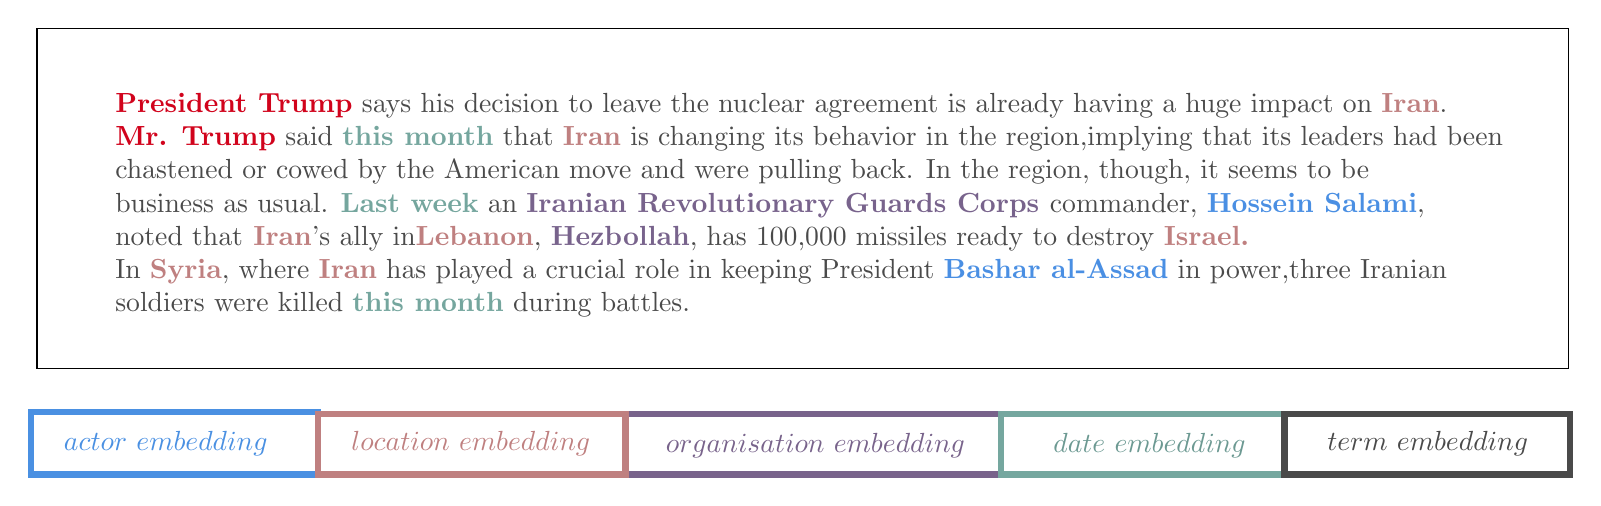
\begin{tikzpicture}[x=0.75pt,y=0.75pt,yscale=-1,xscale=1]
%uncomment if require: \path (0,300); %set diagram left start at 0, and has height of 300

\draw  [color={rgb, 255:red, 74; green, 144; blue, 226 }  ,draw opacity=1 ][line width=2.25]   (13, 207) rectangle (151.5, 237)   ;
\draw  [color={rgb, 255:red, 120; green, 99; blue, 139 }  ,draw opacity=1 ][line width=2.25]   (299.5, 208) rectangle (480.5, 237)   ;
\draw  [color={rgb, 255:red, 191; green, 128; blue, 128 }  ,draw opacity=1 ][line width=2.25]   (151.5, 208) rectangle (299.5, 237)   ;
\draw  [color={rgb, 255:red, 117; green, 167; blue, 159 }  ,draw opacity=1 ][line width=2.25]   (480.5, 208) rectangle (617, 237)   ;
\draw  [color={rgb, 255:red, 74; green, 74; blue, 74 }  ,draw opacity=1 ][line width=2.25]   (617, 208) rectangle (754.5, 237)   ;
\draw    (16, 22) rectangle (754, 186)   ;

\draw (78,222) node [color={rgb, 255:red, 74; green, 144; blue, 226 }  ,opacity=1 ]  {$actor\ embedding$};
\draw (225,222) node [color={rgb, 255:red, 191; green, 128; blue, 128 }  ,opacity=1 ]  {$location\ embedding$};
\draw (391,223) node [color={rgb, 255:red, 120; green, 99; blue, 139 }  ,opacity=1 ]  {$organisation\ embedding$};
\draw (552,223) node [color={rgb, 255:red, 108; green, 153; blue, 146 }  ,opacity=1 ]  {$date\ embedding$};
\draw (686,222) node [color={rgb, 255:red, 74; green, 74; blue, 74 }  ,opacity=1 ]  {$term\ embedding$};
\draw (388,130) node [scale=1,color={rgb, 255:red, 74; green, 74; blue, 74 }  ,opacity=1 ] [align=left] {\textcolor[rgb]{0.82,0.01,0.11}{\textbf{President Trump}} says his decision to leave the nuclear agreement is already having a huge impact on \textcolor[rgb]{0.75,0.5,0.5}{\textbf{Iran}}.\\\textcolor[rgb]{0.82,0.01,0.11}{\textbf{Mr. Trump}} said \textcolor[rgb]{0.46,0.65,0.62}{\textbf{this month}} that \textcolor[rgb]{0.75,0.5,0.5}{\textbf{Iran}} is changing its behavior in the region,implying that its leaders had been \\\textcolor[rgb]{0.29,0.29,0.29}{chastened or cowed by the American move and were pulling back. In the region, though, it seems to be}\\business as usual. \textcolor[rgb]{0.46,0.65,0.62}{\textbf{Last week}} an \textbf{\textcolor[rgb]{0.47,0.39,0.55}{Iranian Revolutionary Guards Corps} }commander, \textcolor[rgb]{0.29,0.56,0.89}{\textbf{Hossein Salami}}, \\noted that\textbf{ \textcolor[rgb]{0.75,0.5,0.5}{Iran}}’s ally in\textcolor[rgb]{0.75,0.5,0.5}{ \textbf{Lebanon}}, \textcolor[rgb]{0.47,0.39,0.55}{\textbf{Hezbollah}}, has 100,000 missiles ready to destroy \textbf{\textcolor[rgb]{0.75,0.5,0.5}{Israel.}} \\In \textcolor[rgb]{0.75,0.5,0.5}{\textbf{Syria}}, where \textcolor[rgb]{0.75,0.5,0.5}{\textbf{Iran}} has played a crucial role in keeping President \textcolor[rgb]{0.29,0.56,0.89}{\textbf{Bashar al-Assad}} in power,three Iranian \\soldiers were killed \textcolor[rgb]{0.46,0.65,0.62}{\textbf{this month}} during battles.\\\\\\};


\end{tikzpicture}

}
\caption{Facetted embedding of  the entity \emph{``Donald Trump"} for a short paragraph. Each part of the embedding corresponds to the relation of the center word to that specific type. Each entity type is illustrated with matching color in text and embedding. }
\label{fig:facetted_emb}
\end{figure} 
In the remainder of this chapter, we experiment with different methods to generate these separable parts. We see in Chapter~\ref{chap:eval} that facetted embeddings although more interpretable, are less likely to perform well on common evaluation tasks. 
\section{Facetted GloVe }\label{sec:facetted_glove}
In the previous chapter, we indicated that the LOAD edge weight captures the corpus relations similar to the co-occurrence matrix and that meaning components can be extracted from them. In this chapter, we use this knowledge to create facetted embeddings from the weighted adjacency matrix of the LOAD network. In the first part, the construction of a weighted adjacency matrix is illustrated followed by the model definition. The proposed model contains two type of cost functions, that are discussed separately in Section~\ref{sec:normal_cost} and~\ref{sec:unified_cost}. 
\subsection{Weighted Adjacency Matrix}\label{sec:adj_matrix}
To learn the embeddings, a weighted adjacency matrix for each type of entity and terms is needed (ACT, LOC, TER, ORG, DAT). The matrices are constructed based on the edge list of the LOAD graph, where the weights can be co-occurrence counts (identical to the GloVe model) or, in our case the usual weight of LOAD. A different adjacency matrix, one for each type, have to be created in order to obtain facetted embeddings. For example, the weighted adjacency matrix for actors contains the edges that have a actors as start nodes and any other type as the end node. Since the network is undirected, the same edge exists in the opposite direction..For instance, an edge between an actor and a term is repeated twice and will be used once to create the actor matrix and once to create the term matrix. More formally the matrices can be constructed as shown in Figure~\ref{fig:co-matrix}, where the entries of the matrices are the edge weights between two words.  
\begin{figure}
\[ACT=
\begin{blockarray}{cccccccc}
 &TER1  & \color{myblue}{ ORG1 } &  TER2  & ACT1 & DAT1 & LOC1 & ... \\
\begin{block}{c(ccccccc)}
  ACT1 &m_{00} & \color{myblue}{ m_{01}}  &  m_{02} & m_{03} & m_{04} &m_{00}& ... \\
  ACT2 & m_{10} & \color{myblue}{ m_{11} } &  m_{12} & m_{13} & m_{14} &m_{15}& ... \\
  ACT3 & m_{20} &  \color{myblue}{m_{21} } &  m_{22} & m_{23} & m_{24} &m_{25}& ... \\
  .. & ... &  \color{myblue}{...}  &  ... & ... & ... &...& ... \\
\end{block}
\end{blockarray}
 \]
\[ORG=
\begin{blockarray}{cccccccc}
 &TER1  & \color{myblue}{ ORG1 } &  TER2  & ACT1 & DAT1 & LOC1 & ... \\
\begin{block}{c(ccccccc)}
  ORG1 &m_{00} & \color{myblue}{ m_{01}}  &  m_{02} & m_{03} & m_{04} &m_{00}& ... \\
  ORG2 & m_{10} & \color{myblue}{ m_{11} } &  m_{12} & m_{13} & m_{14} &m_{15}& ... \\
  ORG3 & m_{20} &  \color{myblue}{m_{21} } &  m_{22} & m_{23} & m_{24} &m_{25}& ... \\
  .. & ... &  \color{myblue}{...}  &  ... & ... & ... &...& ... \\
\end{block}
\end{blockarray}
 \]
 \[DAT=
\begin{blockarray}{cccccccc}
 &TER1  & \color{myblue}{ ORG1 } &  TER2  & ACT1 & DAT1 & LOC1 & ... \\
\begin{block}{c(ccccccc)}
  DAT1 &m_{00} & \color{myblue}{ m_{01}}  &  m_{02} & m_{03} & m_{04} &m_{00}& ... \\
  DAT2 & m_{10} & \color{myblue}{ m_{11} } &  m_{12} & m_{13} & m_{14} &m_{15}& ... \\
  DAT3 & m_{20} &  \color{myblue}{m_{21} } &  m_{22} & m_{23} & m_{24} &m_{25}& ... \\
  .. & ... &  \color{myblue}{...}  &  ... & ... & ... &...& ... \\
\end{block}
\end{blockarray}
 \]
 \caption{Facetted weighted adjacency matrix. For each type of entity a weighted adjacency matrix is create that contains all the entities of that type on the rows and all the words in the vocabulary in the rows. }
 \label{fig:co-matrix}
\end{figure}
The columns marked in blue in matrices $ACT\in R^{V_{ACT}\times V}$ , $ORG\in R^{V_{ORG}\times V}$  and $DAT\in R^{V_{DAT}\times V}$ will be used to learn the actor, organisation and date part of the ORG1 embedding respectively. The completely vocabulary is divide into words belonging into each entity type. As a result, if $V$ is the size of the vocabulary and $V_{ACT}$,$V_{LOC}$ $V_{ORG}$, $V_{DAT}$, and $V_{TER}$  are the number of actors,location, organization, dates, and terms in the graph, we will have $V=V_{ACT}+V_{LOC}+V_{ORG}+V_{DAT}+V_{TER}$. The model will learn an embedding for all entities in the row and all entities in the column of the matrix. In case of a symmetric co-occurrence matrix the model learns the same embedding twice. Nevertheless, in our case the matrices are not symmetric and that leads to a definition of a new cost function, where this asymmetry is taken into account.  
\subsection{Cost Function of Facetted Embeddings}
\label{sec:facetted_embeddings}
With five different adjacency matrices, five different embeddings need to be learned. To train all embeddings, two methods are proposed. First, training five different networks one for each type separately and concatenating the outputs to generate the facetted embeddings. Second, train all the embeddings at once in a single network with a unified cost function. In the following, both methods are described in detail. Yet, the second, method despite the compactness, is slower than optimizing the five separate cost functions. It is worth noting that the switching between the training method has no effect on the quality of the learned embeddings, only the training time.\\
\subsubsection{Separate cost functions}
\label{sec:normal_cost}

The general cost function for a single network is the one used for the GloVe model with minor differences: 

\begin{figure}
{\small 
\tikzset{every picture/.style={line width=0.75pt}} %set default line width to 0.75pt        
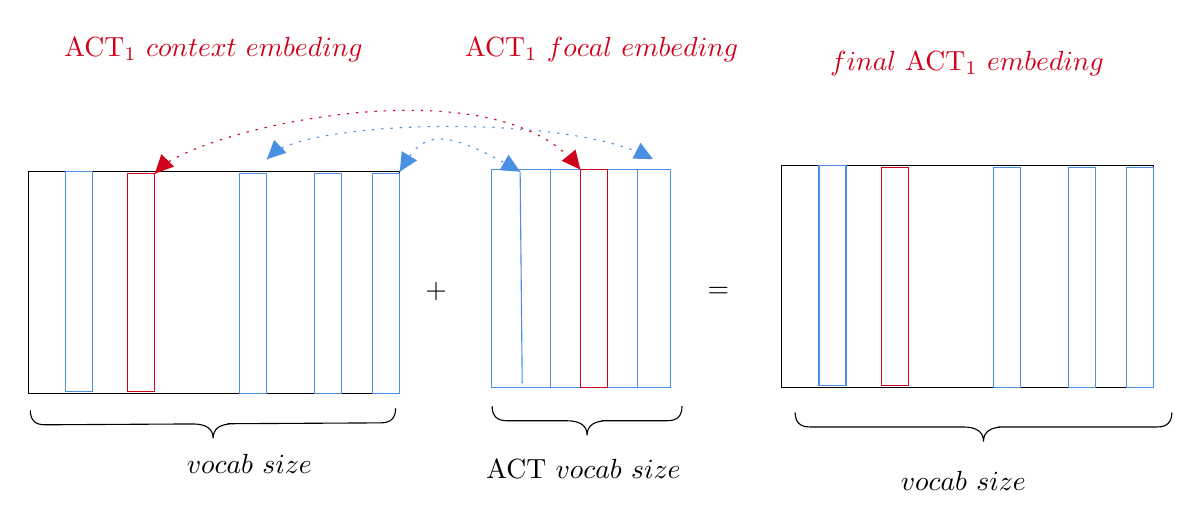
\begin{tikzpicture}[x=0.75pt,y=0.75pt,yscale=-1,xscale=1]
%uncomment if require: \path (0,370); %set diagram left start at 0, and has height of 370

\draw    (16.5, 126) rectangle (195.5, 233)   ;
\draw  [color={rgb, 255:red, 74; green, 144; blue, 226 }  ,draw opacity=1 ]  (239.75, 125) rectangle (326, 230)   ;
\draw   (17.5,241) .. controls (17.53,245.67) and (19.87,247.99) .. (24.54,247.96) -- (95.54,247.55) .. controls (102.21,247.51) and (105.55,249.82) .. (105.58,254.49) .. controls (105.55,249.82) and (108.87,247.47) .. (115.54,247.44)(112.54,247.45) -- (186.54,247.03) .. controls (191.21,247) and (193.53,244.66) .. (193.5,239.99) ;
\draw   (240,239) .. controls (240,243.67) and (242.33,246) .. (247,246) -- (275.75,246) .. controls (282.42,246) and (285.75,248.33) .. (285.75,253) .. controls (285.75,248.33) and (289.08,246) .. (295.75,246)(292.75,246) -- (324.5,246) .. controls (329.17,246) and (331.5,243.67) .. (331.5,239) ;
\draw  [color={rgb, 255:red, 208; green, 2; blue, 27 }  ,draw opacity=1 ]  (64.5, 127) rectangle (77.5, 232)   ;
\draw  [color={rgb, 255:red, 208; green, 2; blue, 27 }  ,draw opacity=1 ]  (282.5, 125) rectangle (295.5, 230)   ;
\draw   (386,242) .. controls (386,246.67) and (388.33,249) .. (393,249) -- (466.75,249) .. controls (473.42,249) and (476.75,251.33) .. (476.75,256) .. controls (476.75,251.33) and (480.08,249) .. (486.75,249)(483.75,249) -- (560.5,249) .. controls (565.17,249) and (567.5,246.67) .. (567.5,242) ;
\draw    (268, 125) rectangle (268, 230)   ;
\draw    (310.25, 125) rectangle (310.25, 229)   ;
\draw [color={rgb, 255:red, 74; green, 144; blue, 226 }  ,draw opacity=1 ]   (253.5,126) -- (254.5,228) ;


\draw [color={rgb, 255:red, 74; green, 144; blue, 226 }  ,draw opacity=1 ]   (268,125) -- (268,230) ;


\draw [color={rgb, 255:red, 74; green, 144; blue, 226 }  ,draw opacity=1 ]   (310.25,125) -- (310.25,230) ;


\draw [color={rgb, 255:red, 74; green, 144; blue, 226 }  ,draw opacity=1 ]   (326,125) -- (326,230) ;


\draw  [color={rgb, 255:red, 74; green, 144; blue, 226 }  ,draw opacity=1 ]  (118.5, 127) rectangle (131.5, 233)   ;
\draw  [color={rgb, 255:red, 74; green, 144; blue, 226 }  ,draw opacity=1 ]  (182.5, 127) rectangle (195.5, 233)   ;
\draw [color={rgb, 255:red, 74; green, 144; blue, 226 }  ,draw opacity=1 ] [dash pattern={on 0.84pt off 2.51pt}]  (195.5,126) .. controls (206.5,107) and (213.5,103) .. (253.5,126) ;
\draw [shift={(253.5,126)}, rotate = 209.57999999999998] [fill={rgb, 255:red, 74; green, 144; blue, 226 }  ,fill opacity=1 ] [draw opacity=0] (8.93,-4.29) -- (0,0) -- (8.93,4.29) -- (8.93,-4.29)    ;
\draw [shift={(195.5,126)}, rotate = 301.28] [fill={rgb, 255:red, 74; green, 144; blue, 226 }  ,fill opacity=1 ] [draw opacity=0] (8.93,-4.29) -- (0,0) -- (8.93,4.29) -- (8.93,-4.29)    ;
\draw [color={rgb, 255:red, 74; green, 144; blue, 226 }  ,draw opacity=1 ] [dash pattern={on 0.84pt off 2.51pt}]  (131.5,120) .. controls (142.5,101) and (277.5,97) .. (317.5,120) ;
\draw [shift={(317.5,120)}, rotate = 207.42000000000002] [fill={rgb, 255:red, 74; green, 144; blue, 226 }  ,fill opacity=1 ] [draw opacity=0] (8.93,-4.29) -- (0,0) -- (8.93,4.29) -- (8.93,-4.29)    ;
\draw [shift={(131.5,120)}, rotate = 316.16] [fill={rgb, 255:red, 74; green, 144; blue, 226 }  ,fill opacity=1 ] [draw opacity=0] (8.93,-4.29) -- (0,0) -- (8.93,4.29) -- (8.93,-4.29)    ;
\draw [color={rgb, 255:red, 208; green, 2; blue, 27 }  ,draw opacity=1 ] [dash pattern={on 0.84pt off 2.51pt}]  (77.5,127) .. controls (88.5,108) and (241.5,70) .. (282.5,125) ;
\draw [shift={(282.5,125)}, rotate = 230.89] [fill={rgb, 255:red, 208; green, 2; blue, 27 }  ,fill opacity=1 ] [draw opacity=0] (8.93,-4.29) -- (0,0) -- (8.93,4.29) -- (8.93,-4.29)    ;
\draw [shift={(77.5,127)}, rotate = 313.85] [fill={rgb, 255:red, 208; green, 2; blue, 27 }  ,fill opacity=1 ] [draw opacity=0] (8.93,-4.29) -- (0,0) -- (8.93,4.29) -- (8.93,-4.29)    ;
\draw  [color={rgb, 255:red, 74; green, 144; blue, 226 }  ,draw opacity=1 ]  (154.5, 127) rectangle (167.5, 233)   ;
\draw  [color={rgb, 255:red, 74; green, 144; blue, 226 }  ,draw opacity=1 ]  (34.5, 126) rectangle (47.5, 232)   ;
\draw    (379.5, 123) rectangle (558.5, 230)   ;
\draw  [color={rgb, 255:red, 208; green, 2; blue, 27 }  ,draw opacity=1 ]  (427.5, 124) rectangle (440.5, 229)   ;
\draw  [color={rgb, 255:red, 74; green, 144; blue, 226 }  ,draw opacity=1 ]  (481.5, 124) rectangle (494.5, 230)   ;
\draw  [color={rgb, 255:red, 74; green, 144; blue, 226 }  ,draw opacity=1 ]  (545.5, 124) rectangle (558.5, 230)   ;
\draw  [color={rgb, 255:red, 74; green, 144; blue, 226 }  ,draw opacity=1 ]  (517.5, 124) rectangle (530.5, 230)   ;
\draw  [color={rgb, 255:red, 74; green, 144; blue, 226 }  ,draw opacity=1 ]  (397.5, 123) rectangle (410.5, 229)   ;

\draw (124,186) node   {$\stackrel{}{}$};
\draw (213,184) node   {$+$};
\draw (349,184) node   {$=$};
\draw (123,267) node   {$vocab\ size$};
\draw (284,269) node   {$\mathrm{ACT}\ vocab\ size$};
\draw (108,67) node [color={rgb, 255:red, 208; green, 2; blue, 27 }  ,opacity=1 ]  {$\mathrm{ACT}_1\ context\ embeding\ $};
\draw (295,67) node [color={rgb, 255:red, 208; green, 2; blue, 27 }  ,opacity=1 ]  {$\mathrm{ACT}_1\ focal\ embeding\ $};
\draw (471,74) node [color={rgb, 255:red, 208; green, 2; blue, 27 }  ,opacity=1 ]  {$final\ \mathrm{ACT}_1\ embeding\ $};
\draw (467,275) node [color={rgb, 255:red, 0; green, 0; blue, 0 }  ,opacity=1 ]  {$vocab\ size$};
\draw (487,183) node   {$\stackrel{}{}$};


\end{tikzpicture}



}
\caption{Selectional addition of focal and context embedding in case of the actor embeddings.} \label{fig:focal_addition}
\end{figure}
\noindent
As noted in the previous section, context and focal embeddings are no longer symmetric like the GloVe model, since the size of context vocabulary is different than the focal. 
By limiting the focal words to a certain type we try to infer the impact of that type on all the words and generate type-specific embeddings. The context embedding in each case reflects these type-specific properties for all words. The biases can no longer be symmetric as well. Therefore, the GloVe cost function can be re-written to Equation~\ref{eq:sep_cost}, where $V_e$ is the size of the focal vocabulary.
\begin{equation}
J_e=\sum _{ j=1 }^{ V }{}\sum _{ i=1 }^{ V_e }{ f({ X }_{ ij } } )(w_{ i }^{ T }\tilde{  w_{ j } } +b_{ i }+\tilde{  b_{ j } } -log{ X }_{ ij })^2
\label{eq:sep_cost}
\end{equation}
The cost function has to be minimized separately for each entity type. As a result, the training will contain five phases, one for each type and a final concatenation. \\
\noindent
\emph{Asymmetry of context and focal embeddings:} Similar to GloVe the embeddings for both context and focal are learned, but the focal embedding can no longer be naively summed up with the context. Instead, the focal embeddings can either be disregarded completely or added in a new way. For this purpose, we propose selectional addition, where the focal embedding of a certain type is only added to the corresponding embedding in the context. As an example, take the adjacency matrices in Section~\ref{sec:adj_matrix} as our input, then for the matrix ACT,  focal embedding will learn to encode each row with an embedding, while the context will encode the columns. The rows of the matrix will represent the embedding of all the actors with respect to the whole vocabulary. We are interested in the column embedding that encodes the actor part for all the words in our vocabulary, which is the purpose of this model. Focal embedding also contains information about the whole vocabulary, but only for the focal words, adding back this information in terms of selectional addition has proven to be beneficial to the model. The selectional addition, adds the focal embedding of a type, only to the respective entities of that type. The rest of embeddings remain intact, because a corresponding embedding column for them in the focal matrix does not exist. A visualization of the addition can be seen in Figure~\ref{fig:focal_addition}.
\noindent
\emph{Final concatenation:}  For each complete embedding, five different context embeddings of types ACT, ORG, DAT, TER, and LOC have to be generated. These vectors can later be combined to generate the complete facetted embedding. As the embeddings are independent, the combination can be arbitrary with only the desired dimensions kept. \\

%\begin{figure}
%\centering 
%\resizebox{0.6\textwidth}{0.6\textwidth}{      
%
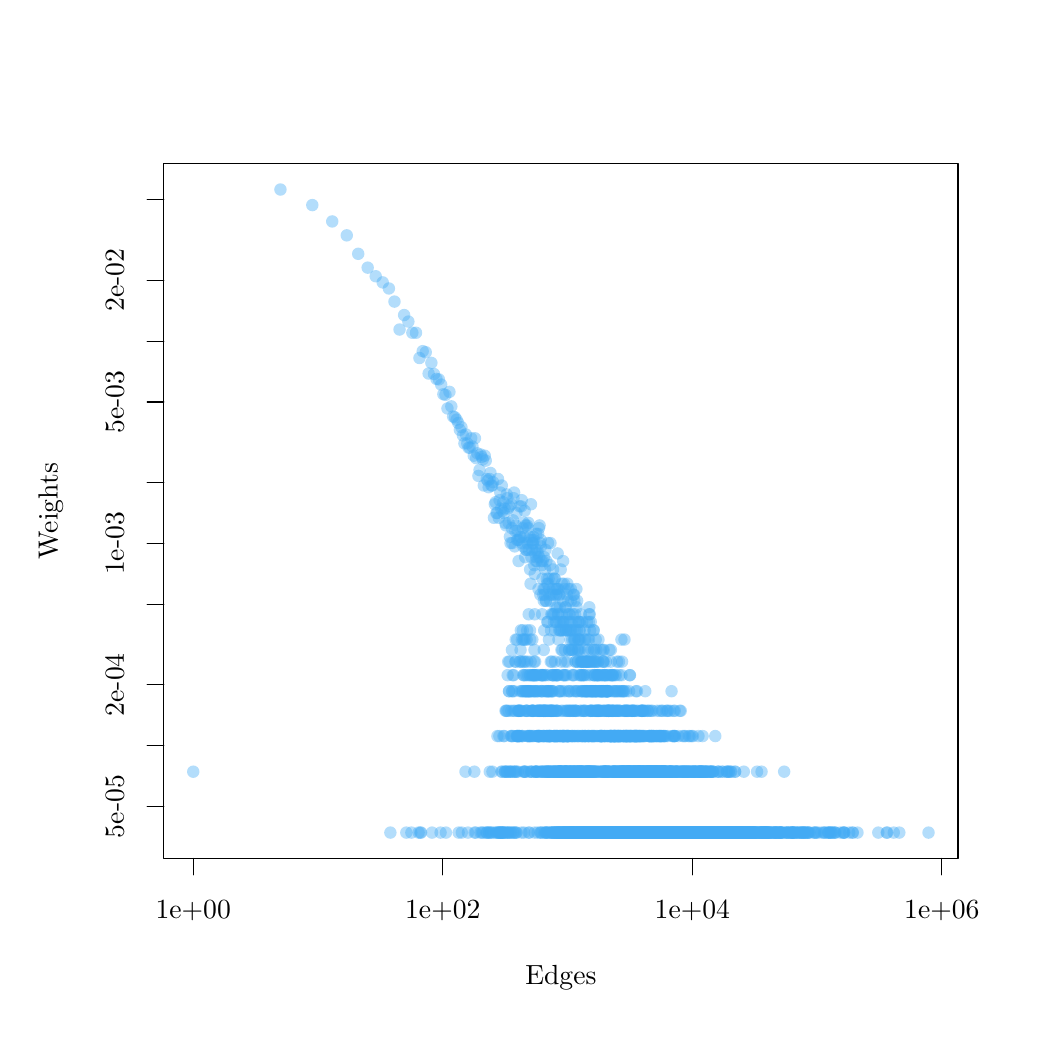
\begin{tikzpicture}[x=1pt,y=1pt]
\definecolor{fillColor}{RGB}{255,255,255}
\path[use as bounding box,fill=fillColor,fill opacity=0.00] (0,0) rectangle (361.35,361.35);
\begin{scope}
\path[clip] ( 49.20, 61.20) rectangle (336.15,312.15);
\definecolor{fillColor}{RGB}{66,170,244}

\path[fill=fillColor,fill opacity=0.40] ( 59.83, 92.50) circle (  2.25);

\path[fill=fillColor,fill opacity=0.40] ( 91.34,302.86) circle (  2.25);

\path[fill=fillColor,fill opacity=0.40] (102.85,297.24) circle (  2.25);

\path[fill=fillColor,fill opacity=0.40] (110.05,291.33) circle (  2.25);

\path[fill=fillColor,fill opacity=0.40] (115.31,286.30) circle (  2.25);

\path[fill=fillColor,fill opacity=0.40] (119.44,279.63) circle (  2.25);

\path[fill=fillColor,fill opacity=0.40] (122.86,274.63) circle (  2.25);

\path[fill=fillColor,fill opacity=0.40] (125.76,271.52) circle (  2.25);

\path[fill=fillColor,fill opacity=0.40] (128.29,269.30) circle (  2.25);

\path[fill=fillColor,fill opacity=0.40] (130.53,267.11) circle (  2.25);

\path[fill=fillColor,fill opacity=0.40] (131.06, 70.49) circle (  2.25);

\path[fill=fillColor,fill opacity=0.40] (132.54,262.37) circle (  2.25);

\path[fill=fillColor,fill opacity=0.40] (134.37,252.27) circle (  2.25);

\path[fill=fillColor,fill opacity=0.40] (136.03,257.50) circle (  2.25);

\path[fill=fillColor,fill opacity=0.40] (136.82, 70.49) circle (  2.25);

\path[fill=fillColor,fill opacity=0.40] (137.57,255.14) circle (  2.25);

\path[fill=fillColor,fill opacity=0.40] (138.65, 70.49) circle (  2.25);

\path[fill=fillColor,fill opacity=0.40] (139.00,251.11) circle (  2.25);

\path[fill=fillColor,fill opacity=0.40] (140.32,251.11) circle (  2.25);

\path[fill=fillColor,fill opacity=0.40] (141.26, 70.49) circle (  2.25);

\path[fill=fillColor,fill opacity=0.40] (141.57,241.98) circle (  2.25);

\path[fill=fillColor,fill opacity=0.40] (141.87, 70.49) circle (  2.25);

\path[fill=fillColor,fill opacity=0.40] (142.16, 70.49) circle (  2.25);

\path[fill=fillColor,fill opacity=0.40] (142.74,244.46) circle (  2.25);

\path[fill=fillColor,fill opacity=0.40] (143.84,244.06) circle (  2.25);

\path[fill=fillColor,fill opacity=0.40] (144.88,236.37) circle (  2.25);

\path[fill=fillColor,fill opacity=0.40] (145.88,240.22) circle (  2.25);

\path[fill=fillColor,fill opacity=0.40] (146.12, 70.49) circle (  2.25);

\path[fill=fillColor,fill opacity=0.40] (146.82,236.19) circle (  2.25);

\path[fill=fillColor,fill opacity=0.40] (147.72,234.43) circle (  2.25);

\path[fill=fillColor,fill opacity=0.40] (148.58,234.25) circle (  2.25);

\path[fill=fillColor,fill opacity=0.40] (149.20, 70.49) circle (  2.25);

\path[fill=fillColor,fill opacity=0.40] (149.41,232.37) circle (  2.25);

\path[fill=fillColor,fill opacity=0.40] (150.20,228.90) circle (  2.25);

\path[fill=fillColor,fill opacity=0.40] (150.96,228.68) circle (  2.25);

\path[fill=fillColor,fill opacity=0.40] (151.14, 70.49) circle (  2.25);

\path[fill=fillColor,fill opacity=0.40] (151.69,223.75) circle (  2.25);

\path[fill=fillColor,fill opacity=0.40] (152.40,229.75) circle (  2.25);

\path[fill=fillColor,fill opacity=0.40] (153.08,224.50) circle (  2.25);

\path[fill=fillColor,fill opacity=0.40] (153.74,220.83) circle (  2.25);

\path[fill=fillColor,fill opacity=0.40] (154.37,220.55) circle (  2.25);

\path[fill=fillColor,fill opacity=0.40] (154.99,219.69) circle (  2.25);

\path[fill=fillColor,fill opacity=0.40] (155.59,218.52) circle (  2.25);

\path[fill=fillColor,fill opacity=0.40] (155.73, 70.49) circle (  2.25);

\path[fill=fillColor,fill opacity=0.40] (156.17,216.03) circle (  2.25);

\path[fill=fillColor,fill opacity=0.40] (156.73,216.98) circle (  2.25);

\path[fill=fillColor,fill opacity=0.40] (156.87, 70.49) circle (  2.25);

\path[fill=fillColor,fill opacity=0.40] (157.28,214.02) circle (  2.25);

\path[fill=fillColor,fill opacity=0.40] (157.81,211.13) circle (  2.25);

\path[fill=fillColor,fill opacity=0.40] (158.20, 92.50) circle (  2.25);

\path[fill=fillColor,fill opacity=0.40] (158.33,214.36) circle (  2.25);

\path[fill=fillColor,fill opacity=0.40] (158.84,211.13) circle (  2.25);

\path[fill=fillColor,fill opacity=0.40] (159.08, 70.49) circle (  2.25);

\path[fill=fillColor,fill opacity=0.40] (159.33,209.58) circle (  2.25);

\path[fill=fillColor,fill opacity=0.40] (159.81,209.58) circle (  2.25);

\path[fill=fillColor,fill opacity=0.40] (160.28,212.97) circle (  2.25);

\path[fill=fillColor,fill opacity=0.40] (160.74,209.98) circle (  2.25);

\path[fill=fillColor,fill opacity=0.40] (161.18,206.68) circle (  2.25);

\path[fill=fillColor,fill opacity=0.40] (161.40, 92.50) circle (  2.25);

\path[fill=fillColor,fill opacity=0.40] (161.51, 70.49) circle (  2.25);

\path[fill=fillColor,fill opacity=0.40] (161.62,212.97) circle (  2.25);

\path[fill=fillColor,fill opacity=0.40] (161.94, 70.49) circle (  2.25);

\path[fill=fillColor,fill opacity=0.40] (162.05,205.80) circle (  2.25);

\path[fill=fillColor,fill opacity=0.40] (162.47,207.54) circle (  2.25);

\path[fill=fillColor,fill opacity=0.40] (162.88,199.38) circle (  2.25);

\path[fill=fillColor,fill opacity=0.40] (163.28,201.49) circle (  2.25);

\path[fill=fillColor,fill opacity=0.40] (163.58, 70.49) circle (  2.25);

\path[fill=fillColor,fill opacity=0.40] (163.67,207.11) circle (  2.25);

\path[fill=fillColor,fill opacity=0.40] (164.06,206.24) circle (  2.25);

\path[fill=fillColor,fill opacity=0.40] (164.15, 70.49) circle (  2.25);

\path[fill=fillColor,fill opacity=0.40] (164.44,205.35) circle (  2.25);

\path[fill=fillColor,fill opacity=0.40] (164.62, 70.49) circle (  2.25);

\path[fill=fillColor,fill opacity=0.40] (164.81,195.91) circle (  2.25);

\path[fill=fillColor,fill opacity=0.40] (165.17,206.68) circle (  2.25);

\path[fill=fillColor,fill opacity=0.40] (165.53,204.89) circle (  2.25);

\path[fill=fillColor,fill opacity=0.40] (165.62, 70.49) circle (  2.25);

\path[fill=fillColor,fill opacity=0.40] (165.88,198.26) circle (  2.25);

\path[fill=fillColor,fill opacity=0.40] (165.97, 70.49) circle (  2.25);

\path[fill=fillColor,fill opacity=0.40] (166.05, 70.49) circle (  2.25);

\path[fill=fillColor,fill opacity=0.40] (166.23,197.69) circle (  2.25);

\path[fill=fillColor,fill opacity=0.40] (166.57,195.29) circle (  2.25);

\path[fill=fillColor,fill opacity=0.40] (166.65, 70.49) circle (  2.25);

\path[fill=fillColor,fill opacity=0.40] (166.73, 70.49) circle (  2.25);

\path[fill=fillColor,fill opacity=0.40] (166.90,198.26) circle (  2.25);

\path[fill=fillColor,fill opacity=0.40] (166.98, 92.50) circle (  2.25);

\path[fill=fillColor,fill opacity=0.40] (167.23,200.45) circle (  2.25);

\path[fill=fillColor,fill opacity=0.40] (167.31, 70.49) circle (  2.25);

\path[fill=fillColor,fill opacity=0.40] (167.47, 70.49) circle (  2.25);

\path[fill=fillColor,fill opacity=0.40] (167.55,195.91) circle (  2.25);

\path[fill=fillColor,fill opacity=0.40] (167.87,195.91) circle (  2.25);

\path[fill=fillColor,fill opacity=0.40] (167.94, 92.50) circle (  2.25);

\path[fill=fillColor,fill opacity=0.40] (168.18,197.11) circle (  2.25);

\path[fill=fillColor,fill opacity=0.40] (168.26, 70.49) circle (  2.25);

\path[fill=fillColor,fill opacity=0.40] (168.49,184.24) circle (  2.25);

\path[fill=fillColor,fill opacity=0.40] (168.79,189.13) circle (  2.25);

\path[fill=fillColor,fill opacity=0.40] (169.09,189.88) circle (  2.25);

\path[fill=fillColor,fill opacity=0.40] (169.23, 70.49) circle (  2.25);

\path[fill=fillColor,fill opacity=0.40] (169.31, 70.49) circle (  2.25);

\path[fill=fillColor,fill opacity=0.40] (169.38,185.96) circle (  2.25);

\path[fill=fillColor,fill opacity=0.40] (169.67,185.96) circle (  2.25);

\path[fill=fillColor,fill opacity=0.40] (169.74,105.37) circle (  2.25);

\path[fill=fillColor,fill opacity=0.40] (169.81, 70.49) circle (  2.25);

\path[fill=fillColor,fill opacity=0.40] (169.95,198.26) circle (  2.25);

\path[fill=fillColor,fill opacity=0.40] (170.16, 70.49) circle (  2.25);

\path[fill=fillColor,fill opacity=0.40] (170.23,184.24) circle (  2.25);

\path[fill=fillColor,fill opacity=0.40] (170.30, 70.49) circle (  2.25);

\path[fill=fillColor,fill opacity=0.40] (170.37, 70.49) circle (  2.25);

\path[fill=fillColor,fill opacity=0.40] (170.44,105.37) circle (  2.25);

\path[fill=fillColor,fill opacity=0.40] (170.51,190.61) circle (  2.25);

\path[fill=fillColor,fill opacity=0.40] (170.58, 70.49) circle (  2.25);

\path[fill=fillColor,fill opacity=0.40] (170.72, 70.49) circle (  2.25);

\path[fill=fillColor,fill opacity=0.40] (170.78,193.37) circle (  2.25);

\path[fill=fillColor,fill opacity=0.40] (170.85, 70.49) circle (  2.25);

\path[fill=fillColor,fill opacity=0.40] (171.05,187.58) circle (  2.25);

\path[fill=fillColor,fill opacity=0.40] (171.19, 92.50) circle (  2.25);

\path[fill=fillColor,fill opacity=0.40] (171.25, 70.49) circle (  2.25);

\path[fill=fillColor,fill opacity=0.40] (171.32,195.91) circle (  2.25);

\path[fill=fillColor,fill opacity=0.40] (171.38, 70.49) circle (  2.25);

\path[fill=fillColor,fill opacity=0.40] (171.45, 92.50) circle (  2.25);

\path[fill=fillColor,fill opacity=0.40] (171.51, 70.49) circle (  2.25);

\path[fill=fillColor,fill opacity=0.40] (171.58,186.78) circle (  2.25);

\path[fill=fillColor,fill opacity=0.40] (171.64, 70.49) circle (  2.25);

\path[fill=fillColor,fill opacity=0.40] (171.71, 70.49) circle (  2.25);

\path[fill=fillColor,fill opacity=0.40] (171.77, 70.49) circle (  2.25);

\path[fill=fillColor,fill opacity=0.40] (171.84,189.88) circle (  2.25);

\path[fill=fillColor,fill opacity=0.40] (171.90,105.37) circle (  2.25);

\path[fill=fillColor,fill opacity=0.40] (172.09,185.96) circle (  2.25);

\path[fill=fillColor,fill opacity=0.40] (172.16, 70.49) circle (  2.25);

\path[fill=fillColor,fill opacity=0.40] (172.28,105.37) circle (  2.25);

\path[fill=fillColor,fill opacity=0.40] (172.35,187.58) circle (  2.25);

\path[fill=fillColor,fill opacity=0.40] (172.41, 92.50) circle (  2.25);

\path[fill=fillColor,fill opacity=0.40] (172.47, 92.50) circle (  2.25);

\path[fill=fillColor,fill opacity=0.40] (172.53, 70.49) circle (  2.25);

\path[fill=fillColor,fill opacity=0.40] (172.59,182.42) circle (  2.25);

\path[fill=fillColor,fill opacity=0.40] (172.66,114.50) circle (  2.25);

\path[fill=fillColor,fill opacity=0.40] (172.72, 92.50) circle (  2.25);

\path[fill=fillColor,fill opacity=0.40] (172.78, 70.49) circle (  2.25);

\path[fill=fillColor,fill opacity=0.40] (172.84,181.48) circle (  2.25);

\path[fill=fillColor,fill opacity=0.40] (172.90,114.50) circle (  2.25);

\path[fill=fillColor,fill opacity=0.40] (173.02, 92.50) circle (  2.25);

\path[fill=fillColor,fill opacity=0.40] (173.08,192.70) circle (  2.25);

\path[fill=fillColor,fill opacity=0.40] (173.14,114.50) circle (  2.25);

\path[fill=fillColor,fill opacity=0.40] (173.26, 92.50) circle (  2.25);

\path[fill=fillColor,fill opacity=0.40] (173.32,191.32) circle (  2.25);

\path[fill=fillColor,fill opacity=0.40] (173.38, 70.49) circle (  2.25);

\path[fill=fillColor,fill opacity=0.40] (173.44,127.37) circle (  2.25);

\path[fill=fillColor,fill opacity=0.40] (173.50, 70.49) circle (  2.25);

\path[fill=fillColor,fill opacity=0.40] (173.56,187.58) circle (  2.25);

\path[fill=fillColor,fill opacity=0.40] (173.62,132.26) circle (  2.25);

\path[fill=fillColor,fill opacity=0.40] (173.68, 70.49) circle (  2.25);

\path[fill=fillColor,fill opacity=0.40] (173.73,114.50) circle (  2.25);

\path[fill=fillColor,fill opacity=0.40] (173.79,182.42) circle (  2.25);

\path[fill=fillColor,fill opacity=0.40] (173.85, 92.50) circle (  2.25);

\path[fill=fillColor,fill opacity=0.40] (173.91,121.58) circle (  2.25);

\path[fill=fillColor,fill opacity=0.40] (173.97,121.58) circle (  2.25);

\path[fill=fillColor,fill opacity=0.40] (174.02,188.37) circle (  2.25);

\path[fill=fillColor,fill opacity=0.40] (174.08,132.26) circle (  2.25);

\path[fill=fillColor,fill opacity=0.40] (174.14, 70.49) circle (  2.25);

\path[fill=fillColor,fill opacity=0.40] (174.25,177.38) circle (  2.25);

\path[fill=fillColor,fill opacity=0.40] (174.31, 92.50) circle (  2.25);

\path[fill=fillColor,fill opacity=0.40] (174.42, 92.50) circle (  2.25);

\path[fill=fillColor,fill opacity=0.40] (174.48,175.11) circle (  2.25);

\path[fill=fillColor,fill opacity=0.40] (174.53, 70.49) circle (  2.25);

\path[fill=fillColor,fill opacity=0.40] (174.59, 92.50) circle (  2.25);

\path[fill=fillColor,fill opacity=0.40] (174.64,105.37) circle (  2.25);

\path[fill=fillColor,fill opacity=0.40] (174.70,189.13) circle (  2.25);

\path[fill=fillColor,fill opacity=0.40] (174.76,114.50) circle (  2.25);

\path[fill=fillColor,fill opacity=0.40] (174.81,105.37) circle (  2.25);

\path[fill=fillColor,fill opacity=0.40] (174.87, 70.49) circle (  2.25);

\path[fill=fillColor,fill opacity=0.40] (174.92,180.50) circle (  2.25);

\path[fill=fillColor,fill opacity=0.40] (174.98,136.50) circle (  2.25);

\path[fill=fillColor,fill opacity=0.40] (175.03,121.58) circle (  2.25);

\path[fill=fillColor,fill opacity=0.40] (175.08,105.37) circle (  2.25);

\path[fill=fillColor,fill opacity=0.40] (175.14,175.11) circle (  2.25);

\path[fill=fillColor,fill opacity=0.40] (175.19,121.58) circle (  2.25);

\path[fill=fillColor,fill opacity=0.40] (175.25,127.37) circle (  2.25);

\path[fill=fillColor,fill opacity=0.40] (175.30, 92.50) circle (  2.25);

\path[fill=fillColor,fill opacity=0.40] (175.35,183.34) circle (  2.25);

\path[fill=fillColor,fill opacity=0.40] (175.41, 70.49) circle (  2.25);

\path[fill=fillColor,fill opacity=0.40] (175.46,105.37) circle (  2.25);

\path[fill=fillColor,fill opacity=0.40] (175.52,114.50) circle (  2.25);

\path[fill=fillColor,fill opacity=0.40] (175.57,191.32) circle (  2.25);

\path[fill=fillColor,fill opacity=0.40] (175.62,127.37) circle (  2.25);

\path[fill=fillColor,fill opacity=0.40] (175.73, 70.49) circle (  2.25);

\path[fill=fillColor,fill opacity=0.40] (175.78,193.37) circle (  2.25);

\path[fill=fillColor,fill opacity=0.40] (175.83,121.58) circle (  2.25);

\path[fill=fillColor,fill opacity=0.40] (175.88, 92.50) circle (  2.25);

\path[fill=fillColor,fill opacity=0.40] (175.94, 92.50) circle (  2.25);

\path[fill=fillColor,fill opacity=0.40] (175.99,173.91) circle (  2.25);

\path[fill=fillColor,fill opacity=0.40] (176.04,114.50) circle (  2.25);

\path[fill=fillColor,fill opacity=0.40] (176.09, 70.49) circle (  2.25);

\path[fill=fillColor,fill opacity=0.40] (176.20,179.49) circle (  2.25);

\path[fill=fillColor,fill opacity=0.40] (176.25,132.26) circle (  2.25);

\path[fill=fillColor,fill opacity=0.40] (176.30,132.26) circle (  2.25);

\path[fill=fillColor,fill opacity=0.40] (176.35,140.24) circle (  2.25);

\path[fill=fillColor,fill opacity=0.40] (176.40,181.48) circle (  2.25);

\path[fill=fillColor,fill opacity=0.40] (176.45, 70.49) circle (  2.25);

\path[fill=fillColor,fill opacity=0.40] (176.50, 92.50) circle (  2.25);

\path[fill=fillColor,fill opacity=0.40] (176.55, 92.50) circle (  2.25);

\path[fill=fillColor,fill opacity=0.40] (176.60,185.96) circle (  2.25);

\path[fill=fillColor,fill opacity=0.40] (176.65, 70.49) circle (  2.25);

\path[fill=fillColor,fill opacity=0.40] (176.70,105.37) circle (  2.25);

\path[fill=fillColor,fill opacity=0.40] (176.75,105.37) circle (  2.25);

\path[fill=fillColor,fill opacity=0.40] (176.80,176.26) circle (  2.25);

\path[fill=fillColor,fill opacity=0.40] (176.85,140.24) circle (  2.25);

\path[fill=fillColor,fill opacity=0.40] (176.90,105.37) circle (  2.25);

\path[fill=fillColor,fill opacity=0.40] (176.95,105.37) circle (  2.25);

\path[fill=fillColor,fill opacity=0.40] (177.00,179.49) circle (  2.25);

\path[fill=fillColor,fill opacity=0.40] (177.05,114.50) circle (  2.25);

\path[fill=fillColor,fill opacity=0.40] (177.10,105.37) circle (  2.25);

\path[fill=fillColor,fill opacity=0.40] (177.15, 92.50) circle (  2.25);

\path[fill=fillColor,fill opacity=0.40] (177.20,176.26) circle (  2.25);

\path[fill=fillColor,fill opacity=0.40] (177.25,105.37) circle (  2.25);

\path[fill=fillColor,fill opacity=0.40] (177.29,114.50) circle (  2.25);

\path[fill=fillColor,fill opacity=0.40] (177.34,114.50) circle (  2.25);

\path[fill=fillColor,fill opacity=0.40] (177.39,168.61) circle (  2.25);

\path[fill=fillColor,fill opacity=0.40] (177.44,114.50) circle (  2.25);

\path[fill=fillColor,fill opacity=0.40] (177.49,105.37) circle (  2.25);

\path[fill=fillColor,fill opacity=0.40] (177.54,114.50) circle (  2.25);

\path[fill=fillColor,fill opacity=0.40] (177.58,176.26) circle (  2.25);

\path[fill=fillColor,fill opacity=0.40] (177.63,105.37) circle (  2.25);

\path[fill=fillColor,fill opacity=0.40] (177.68,105.37) circle (  2.25);

\path[fill=fillColor,fill opacity=0.40] (177.73,114.50) circle (  2.25);

\path[fill=fillColor,fill opacity=0.40] (177.77,188.37) circle (  2.25);

\path[fill=fillColor,fill opacity=0.40] (177.82,132.26) circle (  2.25);

\path[fill=fillColor,fill opacity=0.40] (177.87,105.37) circle (  2.25);

\path[fill=fillColor,fill opacity=0.40] (177.92,114.50) circle (  2.25);

\path[fill=fillColor,fill opacity=0.40] (177.96,177.38) circle (  2.25);

\path[fill=fillColor,fill opacity=0.40] (178.01,121.58) circle (  2.25);

\path[fill=fillColor,fill opacity=0.40] (178.06,132.26) circle (  2.25);

\path[fill=fillColor,fill opacity=0.40] (178.10,136.50) circle (  2.25);

\path[fill=fillColor,fill opacity=0.40] (178.15,177.38) circle (  2.25);

\path[fill=fillColor,fill opacity=0.40] (178.20,143.58) circle (  2.25);

\path[fill=fillColor,fill opacity=0.40] (178.24,114.50) circle (  2.25);

\path[fill=fillColor,fill opacity=0.40] (178.34,188.37) circle (  2.25);

\path[fill=fillColor,fill opacity=0.40] (178.38,114.50) circle (  2.25);

\path[fill=fillColor,fill opacity=0.40] (178.43, 70.49) circle (  2.25);

\path[fill=fillColor,fill opacity=0.40] (178.47,121.58) circle (  2.25);

\path[fill=fillColor,fill opacity=0.40] (178.52,190.61) circle (  2.25);

\path[fill=fillColor,fill opacity=0.40] (178.56,140.24) circle (  2.25);

\path[fill=fillColor,fill opacity=0.40] (178.61,105.37) circle (  2.25);

\path[fill=fillColor,fill opacity=0.40] (178.65,105.37) circle (  2.25);

\path[fill=fillColor,fill opacity=0.40] (178.70,175.11) circle (  2.25);

\path[fill=fillColor,fill opacity=0.40] (178.75,132.26) circle (  2.25);

\path[fill=fillColor,fill opacity=0.40] (178.79,121.58) circle (  2.25);

\path[fill=fillColor,fill opacity=0.40] (178.84,105.37) circle (  2.25);

\path[fill=fillColor,fill opacity=0.40] (178.88,180.50) circle (  2.25);

\path[fill=fillColor,fill opacity=0.40] (178.93,143.58) circle (  2.25);

\path[fill=fillColor,fill opacity=0.40] (178.97,121.58) circle (  2.25);

\path[fill=fillColor,fill opacity=0.40] (179.01, 92.50) circle (  2.25);

\path[fill=fillColor,fill opacity=0.40] (179.06,173.91) circle (  2.25);

\path[fill=fillColor,fill opacity=0.40] (179.10,140.24) circle (  2.25);

\path[fill=fillColor,fill opacity=0.40] (179.15,127.37) circle (  2.25);

\path[fill=fillColor,fill opacity=0.40] (179.19,127.37) circle (  2.25);

\path[fill=fillColor,fill opacity=0.40] (179.24,182.42) circle (  2.25);

\path[fill=fillColor,fill opacity=0.40] (179.28,140.24) circle (  2.25);

\path[fill=fillColor,fill opacity=0.40] (179.32,132.26) circle (  2.25);

\path[fill=fillColor,fill opacity=0.40] (179.37, 70.49) circle (  2.25);

\path[fill=fillColor,fill opacity=0.40] (179.41,177.38) circle (  2.25);

\path[fill=fillColor,fill opacity=0.40] (179.45, 92.50) circle (  2.25);

\path[fill=fillColor,fill opacity=0.40] (179.50,121.58) circle (  2.25);

\path[fill=fillColor,fill opacity=0.40] (179.54, 92.50) circle (  2.25);

\path[fill=fillColor,fill opacity=0.40] (179.58,186.78) circle (  2.25);

\path[fill=fillColor,fill opacity=0.40] (179.63,127.37) circle (  2.25);

\path[fill=fillColor,fill opacity=0.40] (179.67,132.26) circle (  2.25);

\path[fill=fillColor,fill opacity=0.40] (179.71, 92.50) circle (  2.25);

\path[fill=fillColor,fill opacity=0.40] (179.76,170.02) circle (  2.25);

\path[fill=fillColor,fill opacity=0.40] (179.80,140.24) circle (  2.25);

\path[fill=fillColor,fill opacity=0.40] (179.84,121.58) circle (  2.25);

\path[fill=fillColor,fill opacity=0.40] (179.88, 92.50) circle (  2.25);

\path[fill=fillColor,fill opacity=0.40] (179.93,181.48) circle (  2.25);

\path[fill=fillColor,fill opacity=0.40] (179.97,121.58) circle (  2.25);

\path[fill=fillColor,fill opacity=0.40] (180.01,114.50) circle (  2.25);

\path[fill=fillColor,fill opacity=0.40] (180.05,121.58) circle (  2.25);

\path[fill=fillColor,fill opacity=0.40] (180.10,172.66) circle (  2.25);

\path[fill=fillColor,fill opacity=0.40] (180.14,114.50) circle (  2.25);

\path[fill=fillColor,fill opacity=0.40] (180.18,121.58) circle (  2.25);

\path[fill=fillColor,fill opacity=0.40] (180.22,127.37) circle (  2.25);

\path[fill=fillColor,fill opacity=0.40] (180.26,172.66) circle (  2.25);

\path[fill=fillColor,fill opacity=0.40] (180.31,140.24) circle (  2.25);

\path[fill=fillColor,fill opacity=0.40] (180.35,114.50) circle (  2.25);

\path[fill=fillColor,fill opacity=0.40] (180.39,114.50) circle (  2.25);

\path[fill=fillColor,fill opacity=0.40] (180.43,181.48) circle (  2.25);

\path[fill=fillColor,fill opacity=0.40] (180.47,143.58) circle (  2.25);

\path[fill=fillColor,fill opacity=0.40] (180.51,114.50) circle (  2.25);

\path[fill=fillColor,fill opacity=0.40] (180.55,132.26) circle (  2.25);

\path[fill=fillColor,fill opacity=0.40] (180.60,175.11) circle (  2.25);

\path[fill=fillColor,fill opacity=0.40] (180.64,105.37) circle (  2.25);

\path[fill=fillColor,fill opacity=0.40] (180.68,105.37) circle (  2.25);

\path[fill=fillColor,fill opacity=0.40] (180.72,121.58) circle (  2.25);

\path[fill=fillColor,fill opacity=0.40] (180.76,180.50) circle (  2.25);

\path[fill=fillColor,fill opacity=0.40] (180.80,121.58) circle (  2.25);

\path[fill=fillColor,fill opacity=0.40] (180.84,105.37) circle (  2.25);

\path[fill=fillColor,fill opacity=0.40] (180.88,127.37) circle (  2.25);

\path[fill=fillColor,fill opacity=0.40] (180.92,182.42) circle (  2.25);

\path[fill=fillColor,fill opacity=0.40] (180.96, 70.49) circle (  2.25);

\path[fill=fillColor,fill opacity=0.40] (181.00,121.58) circle (  2.25);

\path[fill=fillColor,fill opacity=0.40] (181.04,149.37) circle (  2.25);

\path[fill=fillColor,fill opacity=0.40] (181.08,172.66) circle (  2.25);

\path[fill=fillColor,fill opacity=0.40] (181.12,121.58) circle (  2.25);

\path[fill=fillColor,fill opacity=0.40] (181.16, 92.50) circle (  2.25);

\path[fill=fillColor,fill opacity=0.40] (181.20,105.37) circle (  2.25);

\path[fill=fillColor,fill opacity=0.40] (181.24,176.26) circle (  2.25);

\path[fill=fillColor,fill opacity=0.40] (181.28,121.58) circle (  2.25);

\path[fill=fillColor,fill opacity=0.40] (181.32, 70.49) circle (  2.25);

\path[fill=fillColor,fill opacity=0.40] (181.36,105.37) circle (  2.25);

\path[fill=fillColor,fill opacity=0.40] (181.40,177.38) circle (  2.25);

\path[fill=fillColor,fill opacity=0.40] (181.44,127.37) circle (  2.25);

\path[fill=fillColor,fill opacity=0.40] (181.48,105.37) circle (  2.25);

\path[fill=fillColor,fill opacity=0.40] (181.52,143.58) circle (  2.25);

\path[fill=fillColor,fill opacity=0.40] (181.56,165.58) circle (  2.25);

\path[fill=fillColor,fill opacity=0.40] (181.60,140.24) circle (  2.25);

\path[fill=fillColor,fill opacity=0.40] (181.63,121.58) circle (  2.25);

\path[fill=fillColor,fill opacity=0.40] (181.67,127.37) circle (  2.25);

\path[fill=fillColor,fill opacity=0.40] (181.71,160.42) circle (  2.25);

\path[fill=fillColor,fill opacity=0.40] (181.75,132.26) circle (  2.25);

\path[fill=fillColor,fill opacity=0.40] (181.79,105.37) circle (  2.25);

\path[fill=fillColor,fill opacity=0.40] (181.83,121.58) circle (  2.25);

\path[fill=fillColor,fill opacity=0.40] (181.87,189.13) circle (  2.25);

\path[fill=fillColor,fill opacity=0.40] (181.91,114.50) circle (  2.25);

\path[fill=fillColor,fill opacity=0.40] (181.94, 92.50) circle (  2.25);

\path[fill=fillColor,fill opacity=0.40] (181.98, 92.50) circle (  2.25);

\path[fill=fillColor,fill opacity=0.40] (182.02,170.02) circle (  2.25);

\path[fill=fillColor,fill opacity=0.40] (182.06,105.37) circle (  2.25);

\path[fill=fillColor,fill opacity=0.40] (182.10,121.58) circle (  2.25);

\path[fill=fillColor,fill opacity=0.40] (182.13,114.50) circle (  2.25);

\path[fill=fillColor,fill opacity=0.40] (182.17,176.26) circle (  2.25);

\path[fill=fillColor,fill opacity=0.40] (182.21, 92.50) circle (  2.25);

\path[fill=fillColor,fill opacity=0.40] (182.25,127.37) circle (  2.25);

\path[fill=fillColor,fill opacity=0.40] (182.29,114.50) circle (  2.25);

\path[fill=fillColor,fill opacity=0.40] (182.32,172.66) circle (  2.25);

\path[fill=fillColor,fill opacity=0.40] (182.36,140.24) circle (  2.25);

\path[fill=fillColor,fill opacity=0.40] (182.40,127.37) circle (  2.25);

\path[fill=fillColor,fill opacity=0.40] (182.44,114.50) circle (  2.25);

\path[fill=fillColor,fill opacity=0.40] (182.47,175.11) circle (  2.25);

\path[fill=fillColor,fill opacity=0.40] (182.51,105.37) circle (  2.25);

\path[fill=fillColor,fill opacity=0.40] (182.55,114.50) circle (  2.25);

\path[fill=fillColor,fill opacity=0.40] (182.58,114.50) circle (  2.25);

\path[fill=fillColor,fill opacity=0.40] (182.62,175.11) circle (  2.25);

\path[fill=fillColor,fill opacity=0.40] (182.66,127.37) circle (  2.25);

\path[fill=fillColor,fill opacity=0.40] (182.70,114.50) circle (  2.25);

\path[fill=fillColor,fill opacity=0.40] (182.73,121.58) circle (  2.25);

\path[fill=fillColor,fill opacity=0.40] (182.77,177.38) circle (  2.25);

\path[fill=fillColor,fill opacity=0.40] (182.81,114.50) circle (  2.25);

\path[fill=fillColor,fill opacity=0.40] (182.84,127.37) circle (  2.25);

\path[fill=fillColor,fill opacity=0.40] (182.88,105.37) circle (  2.25);

\path[fill=fillColor,fill opacity=0.40] (182.92,176.26) circle (  2.25);

\path[fill=fillColor,fill opacity=0.40] (182.95,121.58) circle (  2.25);

\path[fill=fillColor,fill opacity=0.40] (182.99,132.26) circle (  2.25);

\path[fill=fillColor,fill opacity=0.40] (183.02,127.37) circle (  2.25);

\path[fill=fillColor,fill opacity=0.40] (183.06,167.13) circle (  2.25);

\path[fill=fillColor,fill opacity=0.40] (183.10,127.37) circle (  2.25);

\path[fill=fillColor,fill opacity=0.40] (183.13,136.50) circle (  2.25);

\path[fill=fillColor,fill opacity=0.40] (183.17, 70.49) circle (  2.25);

\path[fill=fillColor,fill opacity=0.40] (183.20,163.95) circle (  2.25);

\path[fill=fillColor,fill opacity=0.40] (183.24,149.37) circle (  2.25);

\path[fill=fillColor,fill opacity=0.40] (183.28,127.37) circle (  2.25);

\path[fill=fillColor,fill opacity=0.40] (183.35,171.37) circle (  2.25);

\path[fill=fillColor,fill opacity=0.40] (183.38,132.26) circle (  2.25);

\path[fill=fillColor,fill opacity=0.40] (183.42,121.58) circle (  2.25);

\path[fill=fillColor,fill opacity=0.40] (183.45,121.58) circle (  2.25);

\path[fill=fillColor,fill opacity=0.40] (183.49,172.66) circle (  2.25);

\path[fill=fillColor,fill opacity=0.40] (183.53, 92.50) circle (  2.25);

\path[fill=fillColor,fill opacity=0.40] (183.56, 92.50) circle (  2.25);

\path[fill=fillColor,fill opacity=0.40] (183.60, 92.50) circle (  2.25);

\path[fill=fillColor,fill opacity=0.40] (183.63,168.61) circle (  2.25);

\path[fill=fillColor,fill opacity=0.40] (183.67,127.37) circle (  2.25);

\path[fill=fillColor,fill opacity=0.40] (183.70, 92.50) circle (  2.25);

\path[fill=fillColor,fill opacity=0.40] (183.74, 92.50) circle (  2.25);

\path[fill=fillColor,fill opacity=0.40] (183.77,178.45) circle (  2.25);

\path[fill=fillColor,fill opacity=0.40] (183.81,127.37) circle (  2.25);

\path[fill=fillColor,fill opacity=0.40] (183.84,121.58) circle (  2.25);

\path[fill=fillColor,fill opacity=0.40] (183.88, 92.50) circle (  2.25);

\path[fill=fillColor,fill opacity=0.40] (183.91,170.02) circle (  2.25);

\path[fill=fillColor,fill opacity=0.40] (183.95,105.37) circle (  2.25);

\path[fill=fillColor,fill opacity=0.40] (183.98,105.37) circle (  2.25);

\path[fill=fillColor,fill opacity=0.40] (184.01,114.50) circle (  2.25);

\path[fill=fillColor,fill opacity=0.40] (184.05,168.61) circle (  2.25);

\path[fill=fillColor,fill opacity=0.40] (184.08,114.50) circle (  2.25);

\path[fill=fillColor,fill opacity=0.40] (184.12,114.50) circle (  2.25);

\path[fill=fillColor,fill opacity=0.40] (184.15,105.37) circle (  2.25);

\path[fill=fillColor,fill opacity=0.40] (184.19,172.66) circle (  2.25);

\path[fill=fillColor,fill opacity=0.40] (184.22,127.37) circle (  2.25);

\path[fill=fillColor,fill opacity=0.40] (184.25, 70.49) circle (  2.25);

\path[fill=fillColor,fill opacity=0.40] (184.29,121.58) circle (  2.25);

\path[fill=fillColor,fill opacity=0.40] (184.32,171.37) circle (  2.25);

\path[fill=fillColor,fill opacity=0.40] (184.36,105.37) circle (  2.25);

\path[fill=fillColor,fill opacity=0.40] (184.39, 92.50) circle (  2.25);

\path[fill=fillColor,fill opacity=0.40] (184.42,121.58) circle (  2.25);

\path[fill=fillColor,fill opacity=0.40] (184.46,178.45) circle (  2.25);

\path[fill=fillColor,fill opacity=0.40] (184.49,114.50) circle (  2.25);

\path[fill=fillColor,fill opacity=0.40] (184.52,105.37) circle (  2.25);

\path[fill=fillColor,fill opacity=0.40] (184.56,105.37) circle (  2.25);

\path[fill=fillColor,fill opacity=0.40] (184.59,158.50) circle (  2.25);

\path[fill=fillColor,fill opacity=0.40] (184.63,105.37) circle (  2.25);

\path[fill=fillColor,fill opacity=0.40] (184.66,105.37) circle (  2.25);

\path[fill=fillColor,fill opacity=0.40] (184.69,114.50) circle (  2.25);

\path[fill=fillColor,fill opacity=0.40] (184.73,180.50) circle (  2.25);

\path[fill=fillColor,fill opacity=0.40] (184.76,114.50) circle (  2.25);

\path[fill=fillColor,fill opacity=0.40] (184.79,105.37) circle (  2.25);

\path[fill=fillColor,fill opacity=0.40] (184.86,170.02) circle (  2.25);

\path[fill=fillColor,fill opacity=0.40] (184.89,105.37) circle (  2.25);

\path[fill=fillColor,fill opacity=0.40] (184.96,105.37) circle (  2.25);

\path[fill=fillColor,fill opacity=0.40] (184.99,181.48) circle (  2.25);

\path[fill=fillColor,fill opacity=0.40] (185.02,114.50) circle (  2.25);

\path[fill=fillColor,fill opacity=0.40] (185.05,114.50) circle (  2.25);

\path[fill=fillColor,fill opacity=0.40] (185.09, 92.50) circle (  2.25);

\path[fill=fillColor,fill opacity=0.40] (185.12,175.11) circle (  2.25);

\path[fill=fillColor,fill opacity=0.40] (185.15,114.50) circle (  2.25);

\path[fill=fillColor,fill opacity=0.40] (185.19,105.37) circle (  2.25);

\path[fill=fillColor,fill opacity=0.40] (185.25,156.45) circle (  2.25);

\path[fill=fillColor,fill opacity=0.40] (185.28,114.50) circle (  2.25);

\path[fill=fillColor,fill opacity=0.40] (185.31, 70.49) circle (  2.25);

\path[fill=fillColor,fill opacity=0.40] (185.35, 70.49) circle (  2.25);

\path[fill=fillColor,fill opacity=0.40] (185.38,176.26) circle (  2.25);

\path[fill=fillColor,fill opacity=0.40] (185.41,127.37) circle (  2.25);

\path[fill=fillColor,fill opacity=0.40] (185.44, 92.50) circle (  2.25);

\path[fill=fillColor,fill opacity=0.40] (185.48,114.50) circle (  2.25);

\path[fill=fillColor,fill opacity=0.40] (185.51,173.91) circle (  2.25);

\path[fill=fillColor,fill opacity=0.40] (185.54,127.37) circle (  2.25);

\path[fill=fillColor,fill opacity=0.40] (185.57,114.50) circle (  2.25);

\path[fill=fillColor,fill opacity=0.40] (185.60,121.58) circle (  2.25);

\path[fill=fillColor,fill opacity=0.40] (185.63,168.61) circle (  2.25);

\path[fill=fillColor,fill opacity=0.40] (185.67,121.58) circle (  2.25);

\path[fill=fillColor,fill opacity=0.40] (185.70,121.58) circle (  2.25);

\path[fill=fillColor,fill opacity=0.40] (185.73,105.37) circle (  2.25);

\path[fill=fillColor,fill opacity=0.40] (185.76,167.13) circle (  2.25);

\path[fill=fillColor,fill opacity=0.40] (185.79, 92.50) circle (  2.25);

\path[fill=fillColor,fill opacity=0.40] (185.82,127.37) circle (  2.25);

\path[fill=fillColor,fill opacity=0.40] (185.86, 70.49) circle (  2.25);

\path[fill=fillColor,fill opacity=0.40] (185.89,149.37) circle (  2.25);

\path[fill=fillColor,fill opacity=0.40] (185.92,114.50) circle (  2.25);

\path[fill=fillColor,fill opacity=0.40] (185.95, 92.50) circle (  2.25);

\path[fill=fillColor,fill opacity=0.40] (185.98, 92.50) circle (  2.25);

\path[fill=fillColor,fill opacity=0.40] (186.01,162.24) circle (  2.25);

\path[fill=fillColor,fill opacity=0.40] (186.04,127.37) circle (  2.25);

\path[fill=fillColor,fill opacity=0.40] (186.07,105.37) circle (  2.25);

\path[fill=fillColor,fill opacity=0.40] (186.10,121.58) circle (  2.25);

\path[fill=fillColor,fill opacity=0.40] (186.14,168.61) circle (  2.25);

\path[fill=fillColor,fill opacity=0.40] (186.17,127.37) circle (  2.25);

\path[fill=fillColor,fill opacity=0.40] (186.20,127.37) circle (  2.25);

\path[fill=fillColor,fill opacity=0.40] (186.23,105.37) circle (  2.25);

\path[fill=fillColor,fill opacity=0.40] (186.26,156.45) circle (  2.25);

\path[fill=fillColor,fill opacity=0.40] (186.29,114.50) circle (  2.25);

\path[fill=fillColor,fill opacity=0.40] (186.32,114.50) circle (  2.25);

\path[fill=fillColor,fill opacity=0.40] (186.35,114.50) circle (  2.25);

\path[fill=fillColor,fill opacity=0.40] (186.38,158.50) circle (  2.25);

\path[fill=fillColor,fill opacity=0.40] (186.41,114.50) circle (  2.25);

\path[fill=fillColor,fill opacity=0.40] (186.44,114.50) circle (  2.25);

\path[fill=fillColor,fill opacity=0.40] (186.47,136.50) circle (  2.25);

\path[fill=fillColor,fill opacity=0.40] (186.50,154.26) circle (  2.25);

\path[fill=fillColor,fill opacity=0.40] (186.53,105.37) circle (  2.25);

\path[fill=fillColor,fill opacity=0.40] (186.56,105.37) circle (  2.25);

\path[fill=fillColor,fill opacity=0.40] (186.59, 92.50) circle (  2.25);

\path[fill=fillColor,fill opacity=0.40] (186.62,170.02) circle (  2.25);

\path[fill=fillColor,fill opacity=0.40] (186.65,143.58) circle (  2.25);

\path[fill=fillColor,fill opacity=0.40] (186.68,105.37) circle (  2.25);

\path[fill=fillColor,fill opacity=0.40] (186.71, 70.49) circle (  2.25);

\path[fill=fillColor,fill opacity=0.40] (186.74,158.50) circle (  2.25);

\path[fill=fillColor,fill opacity=0.40] (186.77,114.50) circle (  2.25);

\path[fill=fillColor,fill opacity=0.40] (186.80, 92.50) circle (  2.25);

\path[fill=fillColor,fill opacity=0.40] (186.83,114.50) circle (  2.25);

\path[fill=fillColor,fill opacity=0.40] (186.86,156.45) circle (  2.25);

\path[fill=fillColor,fill opacity=0.40] (186.89,114.50) circle (  2.25);

\path[fill=fillColor,fill opacity=0.40] (186.92,121.58) circle (  2.25);

\path[fill=fillColor,fill opacity=0.40] (186.95,114.50) circle (  2.25);

\path[fill=fillColor,fill opacity=0.40] (186.98,165.58) circle (  2.25);

\path[fill=fillColor,fill opacity=0.40] (187.01,127.37) circle (  2.25);

\path[fill=fillColor,fill opacity=0.40] (187.04, 70.49) circle (  2.25);

\path[fill=fillColor,fill opacity=0.40] (187.07, 92.50) circle (  2.25);

\path[fill=fillColor,fill opacity=0.40] (187.10,172.66) circle (  2.25);

\path[fill=fillColor,fill opacity=0.40] (187.13,127.37) circle (  2.25);

\path[fill=fillColor,fill opacity=0.40] (187.16,114.50) circle (  2.25);

\path[fill=fillColor,fill opacity=0.40] (187.19, 92.50) circle (  2.25);

\path[fill=fillColor,fill opacity=0.40] (187.22,154.26) circle (  2.25);

\path[fill=fillColor,fill opacity=0.40] (187.25,114.50) circle (  2.25);

\path[fill=fillColor,fill opacity=0.40] (187.28, 70.49) circle (  2.25);

\path[fill=fillColor,fill opacity=0.40] (187.31,105.37) circle (  2.25);

\path[fill=fillColor,fill opacity=0.40] (187.34,154.26) circle (  2.25);

\path[fill=fillColor,fill opacity=0.40] (187.36,121.58) circle (  2.25);

\path[fill=fillColor,fill opacity=0.40] (187.39, 70.49) circle (  2.25);

\path[fill=fillColor,fill opacity=0.40] (187.42,105.37) circle (  2.25);

\path[fill=fillColor,fill opacity=0.40] (187.45,168.61) circle (  2.25);

\path[fill=fillColor,fill opacity=0.40] (187.48,121.58) circle (  2.25);

\path[fill=fillColor,fill opacity=0.40] (187.51, 92.50) circle (  2.25);

\path[fill=fillColor,fill opacity=0.40] (187.54,114.50) circle (  2.25);

\path[fill=fillColor,fill opacity=0.40] (187.57,162.24) circle (  2.25);

\path[fill=fillColor,fill opacity=0.40] (187.60, 70.49) circle (  2.25);

\path[fill=fillColor,fill opacity=0.40] (187.62, 92.50) circle (  2.25);

\path[fill=fillColor,fill opacity=0.40] (187.65,105.37) circle (  2.25);

\path[fill=fillColor,fill opacity=0.40] (187.68,160.42) circle (  2.25);

\path[fill=fillColor,fill opacity=0.40] (187.71, 92.50) circle (  2.25);

\path[fill=fillColor,fill opacity=0.40] (187.74,114.50) circle (  2.25);

\path[fill=fillColor,fill opacity=0.40] (187.77, 92.50) circle (  2.25);

\path[fill=fillColor,fill opacity=0.40] (187.80,146.61) circle (  2.25);

\path[fill=fillColor,fill opacity=0.40] (187.82,105.37) circle (  2.25);

\path[fill=fillColor,fill opacity=0.40] (187.85, 70.49) circle (  2.25);

\path[fill=fillColor,fill opacity=0.40] (187.88,121.58) circle (  2.25);

\path[fill=fillColor,fill opacity=0.40] (187.91,146.61) circle (  2.25);

\path[fill=fillColor,fill opacity=0.40] (187.94,105.37) circle (  2.25);

\path[fill=fillColor,fill opacity=0.40] (187.97,114.50) circle (  2.25);

\path[fill=fillColor,fill opacity=0.40] (187.99, 92.50) circle (  2.25);

\path[fill=fillColor,fill opacity=0.40] (188.02,175.11) circle (  2.25);

\path[fill=fillColor,fill opacity=0.40] (188.05,121.58) circle (  2.25);

\path[fill=fillColor,fill opacity=0.40] (188.08,121.58) circle (  2.25);

\path[fill=fillColor,fill opacity=0.40] (188.11,114.50) circle (  2.25);

\path[fill=fillColor,fill opacity=0.40] (188.13,160.42) circle (  2.25);

\path[fill=fillColor,fill opacity=0.40] (188.16,105.37) circle (  2.25);

\path[fill=fillColor,fill opacity=0.40] (188.19, 92.50) circle (  2.25);

\path[fill=fillColor,fill opacity=0.40] (188.22,127.37) circle (  2.25);

\path[fill=fillColor,fill opacity=0.40] (188.25,162.24) circle (  2.25);

\path[fill=fillColor,fill opacity=0.40] (188.27, 92.50) circle (  2.25);

\path[fill=fillColor,fill opacity=0.40] (188.30, 92.50) circle (  2.25);

\path[fill=fillColor,fill opacity=0.40] (188.33, 70.49) circle (  2.25);

\path[fill=fillColor,fill opacity=0.40] (188.36,140.24) circle (  2.25);

\path[fill=fillColor,fill opacity=0.40] (188.38,121.58) circle (  2.25);

\path[fill=fillColor,fill opacity=0.40] (188.41,105.37) circle (  2.25);

\path[fill=fillColor,fill opacity=0.40] (188.44,105.37) circle (  2.25);

\path[fill=fillColor,fill opacity=0.40] (188.47,158.50) circle (  2.25);

\path[fill=fillColor,fill opacity=0.40] (188.49,105.37) circle (  2.25);

\path[fill=fillColor,fill opacity=0.40] (188.52,114.50) circle (  2.25);

\path[fill=fillColor,fill opacity=0.40] (188.55,105.37) circle (  2.25);

\path[fill=fillColor,fill opacity=0.40] (188.58,156.45) circle (  2.25);

\path[fill=fillColor,fill opacity=0.40] (188.60,105.37) circle (  2.25);

\path[fill=fillColor,fill opacity=0.40] (188.63, 70.49) circle (  2.25);

\path[fill=fillColor,fill opacity=0.40] (188.66,105.37) circle (  2.25);

\path[fill=fillColor,fill opacity=0.40] (188.68,167.13) circle (  2.25);

\path[fill=fillColor,fill opacity=0.40] (188.71,114.50) circle (  2.25);

\path[fill=fillColor,fill opacity=0.40] (188.74, 92.50) circle (  2.25);

\path[fill=fillColor,fill opacity=0.40] (188.77, 92.50) circle (  2.25);

\path[fill=fillColor,fill opacity=0.40] (188.79,154.26) circle (  2.25);

\path[fill=fillColor,fill opacity=0.40] (188.82,114.50) circle (  2.25);

\path[fill=fillColor,fill opacity=0.40] (188.85,121.58) circle (  2.25);

\path[fill=fillColor,fill opacity=0.40] (188.87, 92.50) circle (  2.25);

\path[fill=fillColor,fill opacity=0.40] (188.90,175.11) circle (  2.25);

\path[fill=fillColor,fill opacity=0.40] (188.93, 92.50) circle (  2.25);

\path[fill=fillColor,fill opacity=0.40] (188.95,114.50) circle (  2.25);

\path[fill=fillColor,fill opacity=0.40] (188.98,105.37) circle (  2.25);

\path[fill=fillColor,fill opacity=0.40] (189.01,132.26) circle (  2.25);

\path[fill=fillColor,fill opacity=0.40] (189.03,105.37) circle (  2.25);

\path[fill=fillColor,fill opacity=0.40] (189.06,121.58) circle (  2.25);

\path[fill=fillColor,fill opacity=0.40] (189.11,143.58) circle (  2.25);

\path[fill=fillColor,fill opacity=0.40] (189.14,114.50) circle (  2.25);

\path[fill=fillColor,fill opacity=0.40] (189.17, 92.50) circle (  2.25);

\path[fill=fillColor,fill opacity=0.40] (189.19,114.50) circle (  2.25);

\path[fill=fillColor,fill opacity=0.40] (189.22,149.37) circle (  2.25);

\path[fill=fillColor,fill opacity=0.40] (189.25,114.50) circle (  2.25);

\path[fill=fillColor,fill opacity=0.40] (189.27, 70.49) circle (  2.25);

\path[fill=fillColor,fill opacity=0.40] (189.30,105.37) circle (  2.25);

\path[fill=fillColor,fill opacity=0.40] (189.33,156.45) circle (  2.25);

\path[fill=fillColor,fill opacity=0.40] (189.35, 70.49) circle (  2.25);

\path[fill=fillColor,fill opacity=0.40] (189.38,114.50) circle (  2.25);

\path[fill=fillColor,fill opacity=0.40] (189.40, 70.49) circle (  2.25);

\path[fill=fillColor,fill opacity=0.40] (189.43,132.26) circle (  2.25);

\path[fill=fillColor,fill opacity=0.40] (189.46,121.58) circle (  2.25);

\path[fill=fillColor,fill opacity=0.40] (189.48, 70.49) circle (  2.25);

\path[fill=fillColor,fill opacity=0.40] (189.51,114.50) circle (  2.25);

\path[fill=fillColor,fill opacity=0.40] (189.54,149.37) circle (  2.25);

\path[fill=fillColor,fill opacity=0.40] (189.56,127.37) circle (  2.25);

\path[fill=fillColor,fill opacity=0.40] (189.59,121.58) circle (  2.25);

\path[fill=fillColor,fill opacity=0.40] (189.61, 92.50) circle (  2.25);

\path[fill=fillColor,fill opacity=0.40] (189.64,162.24) circle (  2.25);

\path[fill=fillColor,fill opacity=0.40] (189.66, 92.50) circle (  2.25);

\path[fill=fillColor,fill opacity=0.40] (189.69,127.37) circle (  2.25);

\path[fill=fillColor,fill opacity=0.40] (189.72,114.50) circle (  2.25);

\path[fill=fillColor,fill opacity=0.40] (189.74,158.50) circle (  2.25);

\path[fill=fillColor,fill opacity=0.40] (189.77,127.37) circle (  2.25);

\path[fill=fillColor,fill opacity=0.40] (189.79, 70.49) circle (  2.25);

\path[fill=fillColor,fill opacity=0.40] (189.82, 70.49) circle (  2.25);

\path[fill=fillColor,fill opacity=0.40] (189.84,165.58) circle (  2.25);

\path[fill=fillColor,fill opacity=0.40] (189.87,121.58) circle (  2.25);

\path[fill=fillColor,fill opacity=0.40] (189.90, 92.50) circle (  2.25);

\path[fill=fillColor,fill opacity=0.40] (189.92,114.50) circle (  2.25);

\path[fill=fillColor,fill opacity=0.40] (189.95,149.37) circle (  2.25);

\path[fill=fillColor,fill opacity=0.40] (190.00,127.37) circle (  2.25);

\path[fill=fillColor,fill opacity=0.40] (190.02,114.50) circle (  2.25);

\path[fill=fillColor,fill opacity=0.40] (190.05,156.45) circle (  2.25);

\path[fill=fillColor,fill opacity=0.40] (190.07,105.37) circle (  2.25);

\path[fill=fillColor,fill opacity=0.40] (190.10, 92.50) circle (  2.25);

\path[fill=fillColor,fill opacity=0.40] (190.12,105.37) circle (  2.25);

\path[fill=fillColor,fill opacity=0.40] (190.15,146.61) circle (  2.25);

\path[fill=fillColor,fill opacity=0.40] (190.17, 92.50) circle (  2.25);

\path[fill=fillColor,fill opacity=0.40] (190.22,105.37) circle (  2.25);

\path[fill=fillColor,fill opacity=0.40] (190.25,149.37) circle (  2.25);

\path[fill=fillColor,fill opacity=0.40] (190.27, 70.49) circle (  2.25);

\path[fill=fillColor,fill opacity=0.40] (190.30, 70.49) circle (  2.25);

\path[fill=fillColor,fill opacity=0.40] (190.33,105.37) circle (  2.25);

\path[fill=fillColor,fill opacity=0.40] (190.35,162.24) circle (  2.25);

\path[fill=fillColor,fill opacity=0.40] (190.37,105.37) circle (  2.25);

\path[fill=fillColor,fill opacity=0.40] (190.40, 92.50) circle (  2.25);

\path[fill=fillColor,fill opacity=0.40] (190.42, 70.49) circle (  2.25);

\path[fill=fillColor,fill opacity=0.40] (190.45,162.24) circle (  2.25);

\path[fill=fillColor,fill opacity=0.40] (190.47,127.37) circle (  2.25);

\path[fill=fillColor,fill opacity=0.40] (190.50, 92.50) circle (  2.25);

\path[fill=fillColor,fill opacity=0.40] (190.52, 70.49) circle (  2.25);

\path[fill=fillColor,fill opacity=0.40] (190.55,143.58) circle (  2.25);

\path[fill=fillColor,fill opacity=0.40] (190.57,132.26) circle (  2.25);

\path[fill=fillColor,fill opacity=0.40] (190.60, 92.50) circle (  2.25);

\path[fill=fillColor,fill opacity=0.40] (190.62,114.50) circle (  2.25);

\path[fill=fillColor,fill opacity=0.40] (190.65,158.50) circle (  2.25);

\path[fill=fillColor,fill opacity=0.40] (190.67, 92.50) circle (  2.25);

\path[fill=fillColor,fill opacity=0.40] (190.70, 92.50) circle (  2.25);

\path[fill=fillColor,fill opacity=0.40] (190.72,105.37) circle (  2.25);

\path[fill=fillColor,fill opacity=0.40] (190.75,151.91) circle (  2.25);

\path[fill=fillColor,fill opacity=0.40] (190.77, 70.49) circle (  2.25);

\path[fill=fillColor,fill opacity=0.40] (190.79,105.37) circle (  2.25);

\path[fill=fillColor,fill opacity=0.40] (190.82,105.37) circle (  2.25);

\path[fill=fillColor,fill opacity=0.40] (190.84,146.61) circle (  2.25);

\path[fill=fillColor,fill opacity=0.40] (190.87, 92.50) circle (  2.25);

\path[fill=fillColor,fill opacity=0.40] (190.89, 70.49) circle (  2.25);

\path[fill=fillColor,fill opacity=0.40] (190.92, 70.49) circle (  2.25);

\path[fill=fillColor,fill opacity=0.40] (190.94,156.45) circle (  2.25);

\path[fill=fillColor,fill opacity=0.40] (190.96,127.37) circle (  2.25);

\path[fill=fillColor,fill opacity=0.40] (190.99, 70.49) circle (  2.25);

\path[fill=fillColor,fill opacity=0.40] (191.04,146.61) circle (  2.25);

\path[fill=fillColor,fill opacity=0.40] (191.06,114.50) circle (  2.25);

\path[fill=fillColor,fill opacity=0.40] (191.08, 70.49) circle (  2.25);

\path[fill=fillColor,fill opacity=0.40] (191.11,127.37) circle (  2.25);

\path[fill=fillColor,fill opacity=0.40] (191.13,156.45) circle (  2.25);

\path[fill=fillColor,fill opacity=0.40] (191.16,105.37) circle (  2.25);

\path[fill=fillColor,fill opacity=0.40] (191.18,114.50) circle (  2.25);

\path[fill=fillColor,fill opacity=0.40] (191.20, 92.50) circle (  2.25);

\path[fill=fillColor,fill opacity=0.40] (191.23,158.50) circle (  2.25);

\path[fill=fillColor,fill opacity=0.40] (191.25,105.37) circle (  2.25);

\path[fill=fillColor,fill opacity=0.40] (191.28,127.37) circle (  2.25);

\path[fill=fillColor,fill opacity=0.40] (191.30,114.50) circle (  2.25);

\path[fill=fillColor,fill opacity=0.40] (191.32,151.91) circle (  2.25);

\path[fill=fillColor,fill opacity=0.40] (191.35,127.37) circle (  2.25);

\path[fill=fillColor,fill opacity=0.40] (191.37,105.37) circle (  2.25);

\path[fill=fillColor,fill opacity=0.40] (191.39, 70.49) circle (  2.25);

\path[fill=fillColor,fill opacity=0.40] (191.42,158.50) circle (  2.25);

\path[fill=fillColor,fill opacity=0.40] (191.44,105.37) circle (  2.25);

\path[fill=fillColor,fill opacity=0.40] (191.47,105.37) circle (  2.25);

\path[fill=fillColor,fill opacity=0.40] (191.49,114.50) circle (  2.25);

\path[fill=fillColor,fill opacity=0.40] (191.51,171.37) circle (  2.25);

\path[fill=fillColor,fill opacity=0.40] (191.54, 70.49) circle (  2.25);

\path[fill=fillColor,fill opacity=0.40] (191.56, 92.50) circle (  2.25);

\path[fill=fillColor,fill opacity=0.40] (191.58, 92.50) circle (  2.25);

\path[fill=fillColor,fill opacity=0.40] (191.61,149.37) circle (  2.25);

\path[fill=fillColor,fill opacity=0.40] (191.63, 92.50) circle (  2.25);

\path[fill=fillColor,fill opacity=0.40] (191.65, 70.49) circle (  2.25);

\path[fill=fillColor,fill opacity=0.40] (191.68,127.37) circle (  2.25);

\path[fill=fillColor,fill opacity=0.40] (191.70,149.37) circle (  2.25);

\path[fill=fillColor,fill opacity=0.40] (191.72, 70.49) circle (  2.25);

\path[fill=fillColor,fill opacity=0.40] (191.75, 70.49) circle (  2.25);

\path[fill=fillColor,fill opacity=0.40] (191.77, 92.50) circle (  2.25);

\path[fill=fillColor,fill opacity=0.40] (191.79,140.24) circle (  2.25);

\path[fill=fillColor,fill opacity=0.40] (191.82, 92.50) circle (  2.25);

\path[fill=fillColor,fill opacity=0.40] (191.84, 92.50) circle (  2.25);

\path[fill=fillColor,fill opacity=0.40] (191.86, 70.49) circle (  2.25);

\path[fill=fillColor,fill opacity=0.40] (191.88,158.50) circle (  2.25);

\path[fill=fillColor,fill opacity=0.40] (191.91, 92.50) circle (  2.25);

\path[fill=fillColor,fill opacity=0.40] (191.93, 70.49) circle (  2.25);

\path[fill=fillColor,fill opacity=0.40] (191.95,121.58) circle (  2.25);

\path[fill=fillColor,fill opacity=0.40] (191.98,156.45) circle (  2.25);

\path[fill=fillColor,fill opacity=0.40] (192.00, 92.50) circle (  2.25);

\path[fill=fillColor,fill opacity=0.40] (192.02,105.37) circle (  2.25);

\path[fill=fillColor,fill opacity=0.40] (192.05, 92.50) circle (  2.25);

\path[fill=fillColor,fill opacity=0.40] (192.07,143.58) circle (  2.25);

\path[fill=fillColor,fill opacity=0.40] (192.09, 70.49) circle (  2.25);

\path[fill=fillColor,fill opacity=0.40] (192.11, 70.49) circle (  2.25);

\path[fill=fillColor,fill opacity=0.40] (192.14, 92.50) circle (  2.25);

\path[fill=fillColor,fill opacity=0.40] (192.16,146.61) circle (  2.25);

\path[fill=fillColor,fill opacity=0.40] (192.18,121.58) circle (  2.25);

\path[fill=fillColor,fill opacity=0.40] (192.20, 92.50) circle (  2.25);

\path[fill=fillColor,fill opacity=0.40] (192.23, 70.49) circle (  2.25);

\path[fill=fillColor,fill opacity=0.40] (192.25,156.45) circle (  2.25);

\path[fill=fillColor,fill opacity=0.40] (192.27, 92.50) circle (  2.25);

\path[fill=fillColor,fill opacity=0.40] (192.30,105.37) circle (  2.25);

\path[fill=fillColor,fill opacity=0.40] (192.32, 70.49) circle (  2.25);

\path[fill=fillColor,fill opacity=0.40] (192.34,151.91) circle (  2.25);

\path[fill=fillColor,fill opacity=0.40] (192.36,105.37) circle (  2.25);

\path[fill=fillColor,fill opacity=0.40] (192.39,121.58) circle (  2.25);

\path[fill=fillColor,fill opacity=0.40] (192.41, 70.49) circle (  2.25);

\path[fill=fillColor,fill opacity=0.40] (192.43,143.58) circle (  2.25);

\path[fill=fillColor,fill opacity=0.40] (192.45, 92.50) circle (  2.25);

\path[fill=fillColor,fill opacity=0.40] (192.48, 92.50) circle (  2.25);

\path[fill=fillColor,fill opacity=0.40] (192.50, 92.50) circle (  2.25);

\path[fill=fillColor,fill opacity=0.40] (192.52,146.61) circle (  2.25);

\path[fill=fillColor,fill opacity=0.40] (192.54, 92.50) circle (  2.25);

\path[fill=fillColor,fill opacity=0.40] (192.56, 92.50) circle (  2.25);

\path[fill=fillColor,fill opacity=0.40] (192.59, 92.50) circle (  2.25);

\path[fill=fillColor,fill opacity=0.40] (192.61,165.58) circle (  2.25);

\path[fill=fillColor,fill opacity=0.40] (192.63, 92.50) circle (  2.25);

\path[fill=fillColor,fill opacity=0.40] (192.65, 70.49) circle (  2.25);

\path[fill=fillColor,fill opacity=0.40] (192.68,105.37) circle (  2.25);

\path[fill=fillColor,fill opacity=0.40] (192.70,143.58) circle (  2.25);

\path[fill=fillColor,fill opacity=0.40] (192.72,105.37) circle (  2.25);

\path[fill=fillColor,fill opacity=0.40] (192.74, 70.49) circle (  2.25);

\path[fill=fillColor,fill opacity=0.40] (192.76, 70.49) circle (  2.25);

\path[fill=fillColor,fill opacity=0.40] (192.79,132.26) circle (  2.25);

\path[fill=fillColor,fill opacity=0.40] (192.81,114.50) circle (  2.25);

\path[fill=fillColor,fill opacity=0.40] (192.85, 92.50) circle (  2.25);

\path[fill=fillColor,fill opacity=0.40] (192.87,136.50) circle (  2.25);

\path[fill=fillColor,fill opacity=0.40] (192.90, 92.50) circle (  2.25);

\path[fill=fillColor,fill opacity=0.40] (192.92, 92.50) circle (  2.25);

\path[fill=fillColor,fill opacity=0.40] (192.94, 92.50) circle (  2.25);

\path[fill=fillColor,fill opacity=0.40] (192.96,149.37) circle (  2.25);

\path[fill=fillColor,fill opacity=0.40] (192.98, 92.50) circle (  2.25);

\path[fill=fillColor,fill opacity=0.40] (193.03, 70.49) circle (  2.25);

\path[fill=fillColor,fill opacity=0.40] (193.05,160.42) circle (  2.25);

\path[fill=fillColor,fill opacity=0.40] (193.07,121.58) circle (  2.25);

\path[fill=fillColor,fill opacity=0.40] (193.09, 92.50) circle (  2.25);

\path[fill=fillColor,fill opacity=0.40] (193.14,143.58) circle (  2.25);

\path[fill=fillColor,fill opacity=0.40] (193.16, 70.49) circle (  2.25);

\path[fill=fillColor,fill opacity=0.40] (193.18,105.37) circle (  2.25);

\path[fill=fillColor,fill opacity=0.40] (193.20,105.37) circle (  2.25);

\path[fill=fillColor,fill opacity=0.40] (193.22,136.50) circle (  2.25);

\path[fill=fillColor,fill opacity=0.40] (193.24,105.37) circle (  2.25);

\path[fill=fillColor,fill opacity=0.40] (193.26, 70.49) circle (  2.25);

\path[fill=fillColor,fill opacity=0.40] (193.29, 70.49) circle (  2.25);

\path[fill=fillColor,fill opacity=0.40] (193.31,146.61) circle (  2.25);

\path[fill=fillColor,fill opacity=0.40] (193.33, 70.49) circle (  2.25);

\path[fill=fillColor,fill opacity=0.40] (193.35,114.50) circle (  2.25);

\path[fill=fillColor,fill opacity=0.40] (193.39,154.26) circle (  2.25);

\path[fill=fillColor,fill opacity=0.40] (193.41,105.37) circle (  2.25);

\path[fill=fillColor,fill opacity=0.40] (193.44, 70.49) circle (  2.25);

\path[fill=fillColor,fill opacity=0.40] (193.46,127.37) circle (  2.25);

\path[fill=fillColor,fill opacity=0.40] (193.48,168.61) circle (  2.25);

\path[fill=fillColor,fill opacity=0.40] (193.50,105.37) circle (  2.25);

\path[fill=fillColor,fill opacity=0.40] (193.52, 92.50) circle (  2.25);

\path[fill=fillColor,fill opacity=0.40] (193.54,105.37) circle (  2.25);

\path[fill=fillColor,fill opacity=0.40] (193.56,146.61) circle (  2.25);

\path[fill=fillColor,fill opacity=0.40] (193.58, 70.49) circle (  2.25);

\path[fill=fillColor,fill opacity=0.40] (193.61, 70.49) circle (  2.25);

\path[fill=fillColor,fill opacity=0.40] (193.63,105.37) circle (  2.25);

\path[fill=fillColor,fill opacity=0.40] (193.65,143.58) circle (  2.25);

\path[fill=fillColor,fill opacity=0.40] (193.67, 92.50) circle (  2.25);

\path[fill=fillColor,fill opacity=0.40] (193.69, 70.49) circle (  2.25);

\path[fill=fillColor,fill opacity=0.40] (193.71, 70.49) circle (  2.25);

\path[fill=fillColor,fill opacity=0.40] (193.73,160.42) circle (  2.25);

\path[fill=fillColor,fill opacity=0.40] (193.75,127.37) circle (  2.25);

\path[fill=fillColor,fill opacity=0.40] (193.77,105.37) circle (  2.25);

\path[fill=fillColor,fill opacity=0.40] (193.79, 70.49) circle (  2.25);

\path[fill=fillColor,fill opacity=0.40] (193.82,146.61) circle (  2.25);

\path[fill=fillColor,fill opacity=0.40] (193.84,105.37) circle (  2.25);

\path[fill=fillColor,fill opacity=0.40] (193.86, 70.49) circle (  2.25);

\path[fill=fillColor,fill opacity=0.40] (193.88, 92.50) circle (  2.25);

\path[fill=fillColor,fill opacity=0.40] (193.90,127.37) circle (  2.25);

\path[fill=fillColor,fill opacity=0.40] (193.92,105.37) circle (  2.25);

\path[fill=fillColor,fill opacity=0.40] (193.94, 92.50) circle (  2.25);

\path[fill=fillColor,fill opacity=0.40] (193.98,158.50) circle (  2.25);

\path[fill=fillColor,fill opacity=0.40] (194.00, 92.50) circle (  2.25);

\path[fill=fillColor,fill opacity=0.40] (194.02, 92.50) circle (  2.25);

\path[fill=fillColor,fill opacity=0.40] (194.04,121.58) circle (  2.25);

\path[fill=fillColor,fill opacity=0.40] (194.07,132.26) circle (  2.25);

\path[fill=fillColor,fill opacity=0.40] (194.09, 92.50) circle (  2.25);

\path[fill=fillColor,fill opacity=0.40] (194.11, 70.49) circle (  2.25);

\path[fill=fillColor,fill opacity=0.40] (194.13,105.37) circle (  2.25);

\path[fill=fillColor,fill opacity=0.40] (194.15,136.50) circle (  2.25);

\path[fill=fillColor,fill opacity=0.40] (194.17, 70.49) circle (  2.25);

\path[fill=fillColor,fill opacity=0.40] (194.19, 70.49) circle (  2.25);

\path[fill=fillColor,fill opacity=0.40] (194.23,151.91) circle (  2.25);

\path[fill=fillColor,fill opacity=0.40] (194.25, 92.50) circle (  2.25);

\path[fill=fillColor,fill opacity=0.40] (194.27, 92.50) circle (  2.25);

\path[fill=fillColor,fill opacity=0.40] (194.29, 92.50) circle (  2.25);

\path[fill=fillColor,fill opacity=0.40] (194.31,127.37) circle (  2.25);

\path[fill=fillColor,fill opacity=0.40] (194.33,114.50) circle (  2.25);

\path[fill=fillColor,fill opacity=0.40] (194.35, 70.49) circle (  2.25);

\path[fill=fillColor,fill opacity=0.40] (194.37,105.37) circle (  2.25);

\path[fill=fillColor,fill opacity=0.40] (194.39,151.91) circle (  2.25);

\path[fill=fillColor,fill opacity=0.40] (194.41, 70.49) circle (  2.25);

\path[fill=fillColor,fill opacity=0.40] (194.43, 92.50) circle (  2.25);

\path[fill=fillColor,fill opacity=0.40] (194.45, 92.50) circle (  2.25);

\path[fill=fillColor,fill opacity=0.40] (194.47,143.58) circle (  2.25);

\path[fill=fillColor,fill opacity=0.40] (194.51, 70.49) circle (  2.25);

\path[fill=fillColor,fill opacity=0.40] (194.53, 70.49) circle (  2.25);

\path[fill=fillColor,fill opacity=0.40] (194.55,143.58) circle (  2.25);

\path[fill=fillColor,fill opacity=0.40] (194.57, 92.50) circle (  2.25);

\path[fill=fillColor,fill opacity=0.40] (194.59, 92.50) circle (  2.25);

\path[fill=fillColor,fill opacity=0.40] (194.61, 70.49) circle (  2.25);

\path[fill=fillColor,fill opacity=0.40] (194.63, 92.50) circle (  2.25);

\path[fill=fillColor,fill opacity=0.40] (194.65,105.37) circle (  2.25);

\path[fill=fillColor,fill opacity=0.40] (194.67, 92.50) circle (  2.25);

\path[fill=fillColor,fill opacity=0.40] (194.69,114.50) circle (  2.25);

\path[fill=fillColor,fill opacity=0.40] (194.71,127.37) circle (  2.25);

\path[fill=fillColor,fill opacity=0.40] (194.73, 92.50) circle (  2.25);

\path[fill=fillColor,fill opacity=0.40] (194.75, 70.49) circle (  2.25);

\path[fill=fillColor,fill opacity=0.40] (194.77, 70.49) circle (  2.25);

\path[fill=fillColor,fill opacity=0.40] (194.79,149.37) circle (  2.25);

\path[fill=fillColor,fill opacity=0.40] (194.81,105.37) circle (  2.25);

\path[fill=fillColor,fill opacity=0.40] (194.83, 92.50) circle (  2.25);

\path[fill=fillColor,fill opacity=0.40] (194.85, 92.50) circle (  2.25);

\path[fill=fillColor,fill opacity=0.40] (194.87,156.45) circle (  2.25);

\path[fill=fillColor,fill opacity=0.40] (194.89,105.37) circle (  2.25);

\path[fill=fillColor,fill opacity=0.40] (194.91, 70.49) circle (  2.25);

\path[fill=fillColor,fill opacity=0.40] (194.93,105.37) circle (  2.25);

\path[fill=fillColor,fill opacity=0.40] (194.95,132.26) circle (  2.25);

\path[fill=fillColor,fill opacity=0.40] (194.97,114.50) circle (  2.25);

\path[fill=fillColor,fill opacity=0.40] (194.99, 92.50) circle (  2.25);

\path[fill=fillColor,fill opacity=0.40] (195.03,160.42) circle (  2.25);

\path[fill=fillColor,fill opacity=0.40] (195.05,105.37) circle (  2.25);

\path[fill=fillColor,fill opacity=0.40] (195.07, 70.49) circle (  2.25);

\path[fill=fillColor,fill opacity=0.40] (195.09,105.37) circle (  2.25);

\path[fill=fillColor,fill opacity=0.40] (195.11,143.58) circle (  2.25);

\path[fill=fillColor,fill opacity=0.40] (195.17, 70.49) circle (  2.25);

\path[fill=fillColor,fill opacity=0.40] (195.19,154.26) circle (  2.25);

\path[fill=fillColor,fill opacity=0.40] (195.21, 92.50) circle (  2.25);

\path[fill=fillColor,fill opacity=0.40] (195.25, 70.49) circle (  2.25);

\path[fill=fillColor,fill opacity=0.40] (195.27,146.61) circle (  2.25);

\path[fill=fillColor,fill opacity=0.40] (195.28,105.37) circle (  2.25);

\path[fill=fillColor,fill opacity=0.40] (195.30,114.50) circle (  2.25);

\path[fill=fillColor,fill opacity=0.40] (195.34,143.58) circle (  2.25);

\path[fill=fillColor,fill opacity=0.40] (195.36, 70.49) circle (  2.25);

\path[fill=fillColor,fill opacity=0.40] (195.38,105.37) circle (  2.25);

\path[fill=fillColor,fill opacity=0.40] (195.40, 70.49) circle (  2.25);

\path[fill=fillColor,fill opacity=0.40] (195.42,158.50) circle (  2.25);

\path[fill=fillColor,fill opacity=0.40] (195.44, 70.49) circle (  2.25);

\path[fill=fillColor,fill opacity=0.40] (195.46,105.37) circle (  2.25);

\path[fill=fillColor,fill opacity=0.40] (195.48, 70.49) circle (  2.25);

\path[fill=fillColor,fill opacity=0.40] (195.50,121.58) circle (  2.25);

\path[fill=fillColor,fill opacity=0.40] (195.52,121.58) circle (  2.25);

\path[fill=fillColor,fill opacity=0.40] (195.54, 92.50) circle (  2.25);

\path[fill=fillColor,fill opacity=0.40] (195.55,105.37) circle (  2.25);

\path[fill=fillColor,fill opacity=0.40] (195.57,136.50) circle (  2.25);

\path[fill=fillColor,fill opacity=0.40] (195.59, 70.49) circle (  2.25);

\path[fill=fillColor,fill opacity=0.40] (195.65,149.37) circle (  2.25);

\path[fill=fillColor,fill opacity=0.40] (195.69, 92.50) circle (  2.25);

\path[fill=fillColor,fill opacity=0.40] (195.73,136.50) circle (  2.25);

\path[fill=fillColor,fill opacity=0.40] (195.74,114.50) circle (  2.25);

\path[fill=fillColor,fill opacity=0.40] (195.76, 92.50) circle (  2.25);

\path[fill=fillColor,fill opacity=0.40] (195.78, 92.50) circle (  2.25);

\path[fill=fillColor,fill opacity=0.40] (195.80,149.37) circle (  2.25);

\path[fill=fillColor,fill opacity=0.40] (195.82, 70.49) circle (  2.25);

\path[fill=fillColor,fill opacity=0.40] (195.84, 70.49) circle (  2.25);

\path[fill=fillColor,fill opacity=0.40] (195.86, 70.49) circle (  2.25);

\path[fill=fillColor,fill opacity=0.40] (195.88, 92.50) circle (  2.25);

\path[fill=fillColor,fill opacity=0.40] (195.90, 70.49) circle (  2.25);

\path[fill=fillColor,fill opacity=0.40] (195.91, 70.49) circle (  2.25);

\path[fill=fillColor,fill opacity=0.40] (195.93, 70.49) circle (  2.25);

\path[fill=fillColor,fill opacity=0.40] (195.95,146.61) circle (  2.25);

\path[fill=fillColor,fill opacity=0.40] (195.97, 92.50) circle (  2.25);

\path[fill=fillColor,fill opacity=0.40] (196.01,114.50) circle (  2.25);

\path[fill=fillColor,fill opacity=0.40] (196.03,140.24) circle (  2.25);

\path[fill=fillColor,fill opacity=0.40] (196.05, 92.50) circle (  2.25);

\path[fill=fillColor,fill opacity=0.40] (196.06,114.50) circle (  2.25);

\path[fill=fillColor,fill opacity=0.40] (196.08, 92.50) circle (  2.25);

\path[fill=fillColor,fill opacity=0.40] (196.10,143.58) circle (  2.25);

\path[fill=fillColor,fill opacity=0.40] (196.14, 92.50) circle (  2.25);

\path[fill=fillColor,fill opacity=0.40] (196.16,105.37) circle (  2.25);

\path[fill=fillColor,fill opacity=0.40] (196.18,121.58) circle (  2.25);

\path[fill=fillColor,fill opacity=0.40] (196.19, 70.49) circle (  2.25);

\path[fill=fillColor,fill opacity=0.40] (196.21, 92.50) circle (  2.25);

\path[fill=fillColor,fill opacity=0.40] (196.23, 70.49) circle (  2.25);

\path[fill=fillColor,fill opacity=0.40] (196.25,158.50) circle (  2.25);

\path[fill=fillColor,fill opacity=0.40] (196.27, 92.50) circle (  2.25);

\path[fill=fillColor,fill opacity=0.40] (196.30, 70.49) circle (  2.25);

\path[fill=fillColor,fill opacity=0.40] (196.32,154.26) circle (  2.25);

\path[fill=fillColor,fill opacity=0.40] (196.34, 70.49) circle (  2.25);

\path[fill=fillColor,fill opacity=0.40] (196.36, 70.49) circle (  2.25);

\path[fill=fillColor,fill opacity=0.40] (196.40,143.58) circle (  2.25);

\path[fill=fillColor,fill opacity=0.40] (196.41, 70.49) circle (  2.25);

\path[fill=fillColor,fill opacity=0.40] (196.43, 70.49) circle (  2.25);

\path[fill=fillColor,fill opacity=0.40] (196.45, 70.49) circle (  2.25);

\path[fill=fillColor,fill opacity=0.40] (196.47,136.50) circle (  2.25);

\path[fill=fillColor,fill opacity=0.40] (196.49, 92.50) circle (  2.25);

\path[fill=fillColor,fill opacity=0.40] (196.51, 92.50) circle (  2.25);

\path[fill=fillColor,fill opacity=0.40] (196.54,146.61) circle (  2.25);

\path[fill=fillColor,fill opacity=0.40] (196.56, 70.49) circle (  2.25);

\path[fill=fillColor,fill opacity=0.40] (196.60, 70.49) circle (  2.25);

\path[fill=fillColor,fill opacity=0.40] (196.62,105.37) circle (  2.25);

\path[fill=fillColor,fill opacity=0.40] (196.63,105.37) circle (  2.25);

\path[fill=fillColor,fill opacity=0.40] (196.65, 70.49) circle (  2.25);

\path[fill=fillColor,fill opacity=0.40] (196.67, 70.49) circle (  2.25);

\path[fill=fillColor,fill opacity=0.40] (196.69,136.50) circle (  2.25);

\path[fill=fillColor,fill opacity=0.40] (196.71, 70.49) circle (  2.25);

\path[fill=fillColor,fill opacity=0.40] (196.72, 70.49) circle (  2.25);

\path[fill=fillColor,fill opacity=0.40] (196.74,114.50) circle (  2.25);

\path[fill=fillColor,fill opacity=0.40] (196.76,140.24) circle (  2.25);

\path[fill=fillColor,fill opacity=0.40] (196.78,114.50) circle (  2.25);

\path[fill=fillColor,fill opacity=0.40] (196.80, 70.49) circle (  2.25);

\path[fill=fillColor,fill opacity=0.40] (196.81, 70.49) circle (  2.25);

\path[fill=fillColor,fill opacity=0.40] (196.83,127.37) circle (  2.25);

\path[fill=fillColor,fill opacity=0.40] (196.85, 70.49) circle (  2.25);

\path[fill=fillColor,fill opacity=0.40] (196.87, 70.49) circle (  2.25);

\path[fill=fillColor,fill opacity=0.40] (196.90,136.50) circle (  2.25);

\path[fill=fillColor,fill opacity=0.40] (196.92,105.37) circle (  2.25);

\path[fill=fillColor,fill opacity=0.40] (196.94, 70.49) circle (  2.25);

\path[fill=fillColor,fill opacity=0.40] (196.96,105.37) circle (  2.25);

\path[fill=fillColor,fill opacity=0.40] (196.97,149.37) circle (  2.25);

\path[fill=fillColor,fill opacity=0.40] (196.99, 92.50) circle (  2.25);

\path[fill=fillColor,fill opacity=0.40] (197.01, 70.49) circle (  2.25);

\path[fill=fillColor,fill opacity=0.40] (197.03, 92.50) circle (  2.25);

\path[fill=fillColor,fill opacity=0.40] (197.05,143.58) circle (  2.25);

\path[fill=fillColor,fill opacity=0.40] (197.06, 92.50) circle (  2.25);

\path[fill=fillColor,fill opacity=0.40] (197.08, 70.49) circle (  2.25);

\path[fill=fillColor,fill opacity=0.40] (197.10, 70.49) circle (  2.25);

\path[fill=fillColor,fill opacity=0.40] (197.12,127.37) circle (  2.25);

\path[fill=fillColor,fill opacity=0.40] (197.13,114.50) circle (  2.25);

\path[fill=fillColor,fill opacity=0.40] (197.15, 92.50) circle (  2.25);

\path[fill=fillColor,fill opacity=0.40] (197.17, 70.49) circle (  2.25);

\path[fill=fillColor,fill opacity=0.40] (197.19,156.45) circle (  2.25);

\path[fill=fillColor,fill opacity=0.40] (197.20, 92.50) circle (  2.25);

\path[fill=fillColor,fill opacity=0.40] (197.22, 70.49) circle (  2.25);

\path[fill=fillColor,fill opacity=0.40] (197.24, 70.49) circle (  2.25);

\path[fill=fillColor,fill opacity=0.40] (197.26,121.58) circle (  2.25);

\path[fill=fillColor,fill opacity=0.40] (197.29, 70.49) circle (  2.25);

\path[fill=fillColor,fill opacity=0.40] (197.31, 70.49) circle (  2.25);

\path[fill=fillColor,fill opacity=0.40] (197.33,140.24) circle (  2.25);

\path[fill=fillColor,fill opacity=0.40] (197.34, 70.49) circle (  2.25);

\path[fill=fillColor,fill opacity=0.40] (197.40,156.45) circle (  2.25);

\path[fill=fillColor,fill opacity=0.40] (197.41,114.50) circle (  2.25);

\path[fill=fillColor,fill opacity=0.40] (197.43, 92.50) circle (  2.25);

\path[fill=fillColor,fill opacity=0.40] (197.45, 92.50) circle (  2.25);

\path[fill=fillColor,fill opacity=0.40] (197.47,127.37) circle (  2.25);

\path[fill=fillColor,fill opacity=0.40] (197.48, 92.50) circle (  2.25);

\path[fill=fillColor,fill opacity=0.40] (197.50,105.37) circle (  2.25);

\path[fill=fillColor,fill opacity=0.40] (197.54,154.26) circle (  2.25);

\path[fill=fillColor,fill opacity=0.40] (197.55, 92.50) circle (  2.25);

\path[fill=fillColor,fill opacity=0.40] (197.59, 70.49) circle (  2.25);

\path[fill=fillColor,fill opacity=0.40] (197.60,140.24) circle (  2.25);

\path[fill=fillColor,fill opacity=0.40] (197.62, 92.50) circle (  2.25);

\path[fill=fillColor,fill opacity=0.40] (197.64,105.37) circle (  2.25);

\path[fill=fillColor,fill opacity=0.40] (197.66, 70.49) circle (  2.25);

\path[fill=fillColor,fill opacity=0.40] (197.67,136.50) circle (  2.25);

\path[fill=fillColor,fill opacity=0.40] (197.69, 92.50) circle (  2.25);

\path[fill=fillColor,fill opacity=0.40] (197.71, 70.49) circle (  2.25);

\path[fill=fillColor,fill opacity=0.40] (197.74,140.24) circle (  2.25);

\path[fill=fillColor,fill opacity=0.40] (197.76, 92.50) circle (  2.25);

\path[fill=fillColor,fill opacity=0.40] (197.79, 92.50) circle (  2.25);

\path[fill=fillColor,fill opacity=0.40] (197.81,149.37) circle (  2.25);

\path[fill=fillColor,fill opacity=0.40] (197.86,105.37) circle (  2.25);

\path[fill=fillColor,fill opacity=0.40] (197.88,143.58) circle (  2.25);

\path[fill=fillColor,fill opacity=0.40] (197.91, 70.49) circle (  2.25);

\path[fill=fillColor,fill opacity=0.40] (197.93, 70.49) circle (  2.25);

\path[fill=fillColor,fill opacity=0.40] (197.95,132.26) circle (  2.25);

\path[fill=fillColor,fill opacity=0.40] (197.96,114.50) circle (  2.25);

\path[fill=fillColor,fill opacity=0.40] (198.00,114.50) circle (  2.25);

\path[fill=fillColor,fill opacity=0.40] (198.01,132.26) circle (  2.25);

\path[fill=fillColor,fill opacity=0.40] (198.05, 70.49) circle (  2.25);

\path[fill=fillColor,fill opacity=0.40] (198.08,146.61) circle (  2.25);

\path[fill=fillColor,fill opacity=0.40] (198.10, 70.49) circle (  2.25);

\path[fill=fillColor,fill opacity=0.40] (198.15,121.58) circle (  2.25);

\path[fill=fillColor,fill opacity=0.40] (198.16,114.50) circle (  2.25);

\path[fill=fillColor,fill opacity=0.40] (198.18, 70.49) circle (  2.25);

\path[fill=fillColor,fill opacity=0.40] (198.21,121.58) circle (  2.25);

\path[fill=fillColor,fill opacity=0.40] (198.23,114.50) circle (  2.25);

\path[fill=fillColor,fill opacity=0.40] (198.26, 70.49) circle (  2.25);

\path[fill=fillColor,fill opacity=0.40] (198.28,158.50) circle (  2.25);

\path[fill=fillColor,fill opacity=0.40] (198.30, 70.49) circle (  2.25);

\path[fill=fillColor,fill opacity=0.40] (198.35,151.91) circle (  2.25);

\path[fill=fillColor,fill opacity=0.40] (198.38, 70.49) circle (  2.25);

\path[fill=fillColor,fill opacity=0.40] (198.40, 70.49) circle (  2.25);

\path[fill=fillColor,fill opacity=0.40] (198.41, 92.50) circle (  2.25);

\path[fill=fillColor,fill opacity=0.40] (198.43, 92.50) circle (  2.25);

\path[fill=fillColor,fill opacity=0.40] (198.45,105.37) circle (  2.25);

\path[fill=fillColor,fill opacity=0.40] (198.48,143.58) circle (  2.25);

\path[fill=fillColor,fill opacity=0.40] (198.50, 92.50) circle (  2.25);

\path[fill=fillColor,fill opacity=0.40] (198.51, 92.50) circle (  2.25);

\path[fill=fillColor,fill opacity=0.40] (198.53, 70.49) circle (  2.25);

\path[fill=fillColor,fill opacity=0.40] (198.55,154.26) circle (  2.25);

\path[fill=fillColor,fill opacity=0.40] (198.58, 92.50) circle (  2.25);

\path[fill=fillColor,fill opacity=0.40] (198.59, 70.49) circle (  2.25);

\path[fill=fillColor,fill opacity=0.40] (198.61,136.50) circle (  2.25);

\path[fill=fillColor,fill opacity=0.40] (198.63, 70.49) circle (  2.25);

\path[fill=fillColor,fill opacity=0.40] (198.66,105.37) circle (  2.25);

\path[fill=fillColor,fill opacity=0.40] (198.68,132.26) circle (  2.25);

\path[fill=fillColor,fill opacity=0.40] (198.69, 92.50) circle (  2.25);

\path[fill=fillColor,fill opacity=0.40] (198.71, 70.49) circle (  2.25);

\path[fill=fillColor,fill opacity=0.40] (198.73, 92.50) circle (  2.25);

\path[fill=fillColor,fill opacity=0.40] (198.74,121.58) circle (  2.25);

\path[fill=fillColor,fill opacity=0.40] (198.77, 92.50) circle (  2.25);

\path[fill=fillColor,fill opacity=0.40] (198.79, 70.49) circle (  2.25);

\path[fill=fillColor,fill opacity=0.40] (198.81,132.26) circle (  2.25);

\path[fill=fillColor,fill opacity=0.40] (198.82, 70.49) circle (  2.25);

\path[fill=fillColor,fill opacity=0.40] (198.84, 70.49) circle (  2.25);

\path[fill=fillColor,fill opacity=0.40] (198.85, 92.50) circle (  2.25);

\path[fill=fillColor,fill opacity=0.40] (198.87,136.50) circle (  2.25);

\path[fill=fillColor,fill opacity=0.40] (198.90, 92.50) circle (  2.25);

\path[fill=fillColor,fill opacity=0.40] (198.94,140.24) circle (  2.25);

\path[fill=fillColor,fill opacity=0.40] (198.95,105.37) circle (  2.25);

\path[fill=fillColor,fill opacity=0.40] (198.97, 70.49) circle (  2.25);

\path[fill=fillColor,fill opacity=0.40] (199.00,146.61) circle (  2.25);

\path[fill=fillColor,fill opacity=0.40] (199.03, 70.49) circle (  2.25);

\path[fill=fillColor,fill opacity=0.40] (199.05, 92.50) circle (  2.25);

\path[fill=fillColor,fill opacity=0.40] (199.06,140.24) circle (  2.25);

\path[fill=fillColor,fill opacity=0.40] (199.13,136.50) circle (  2.25);

\path[fill=fillColor,fill opacity=0.40] (199.14,105.37) circle (  2.25);

\path[fill=fillColor,fill opacity=0.40] (199.16, 70.49) circle (  2.25);

\path[fill=fillColor,fill opacity=0.40] (199.19,146.61) circle (  2.25);

\path[fill=fillColor,fill opacity=0.40] (199.24, 92.50) circle (  2.25);

\path[fill=fillColor,fill opacity=0.40] (199.25,140.24) circle (  2.25);

\path[fill=fillColor,fill opacity=0.40] (199.29, 70.49) circle (  2.25);

\path[fill=fillColor,fill opacity=0.40] (199.32,127.37) circle (  2.25);

\path[fill=fillColor,fill opacity=0.40] (199.35, 70.49) circle (  2.25);

\path[fill=fillColor,fill opacity=0.40] (199.37, 92.50) circle (  2.25);

\path[fill=fillColor,fill opacity=0.40] (199.38,143.58) circle (  2.25);

\path[fill=fillColor,fill opacity=0.40] (199.41, 92.50) circle (  2.25);

\path[fill=fillColor,fill opacity=0.40] (199.43, 92.50) circle (  2.25);

\path[fill=fillColor,fill opacity=0.40] (199.44,143.58) circle (  2.25);

\path[fill=fillColor,fill opacity=0.40] (199.46, 70.49) circle (  2.25);

\path[fill=fillColor,fill opacity=0.40] (199.48, 70.49) circle (  2.25);

\path[fill=fillColor,fill opacity=0.40] (199.49, 70.49) circle (  2.25);

\path[fill=fillColor,fill opacity=0.40] (199.51,146.61) circle (  2.25);

\path[fill=fillColor,fill opacity=0.40] (199.52, 92.50) circle (  2.25);

\path[fill=fillColor,fill opacity=0.40] (199.55, 70.49) circle (  2.25);

\path[fill=fillColor,fill opacity=0.40] (199.57,136.50) circle (  2.25);

\path[fill=fillColor,fill opacity=0.40] (199.58, 70.49) circle (  2.25);

\path[fill=fillColor,fill opacity=0.40] (199.62,105.37) circle (  2.25);

\path[fill=fillColor,fill opacity=0.40] (199.63,114.50) circle (  2.25);

\path[fill=fillColor,fill opacity=0.40] (199.65, 92.50) circle (  2.25);

\path[fill=fillColor,fill opacity=0.40] (199.66, 92.50) circle (  2.25);

\path[fill=fillColor,fill opacity=0.40] (199.68, 92.50) circle (  2.25);

\path[fill=fillColor,fill opacity=0.40] (199.69,140.24) circle (  2.25);

\path[fill=fillColor,fill opacity=0.40] (199.71, 70.49) circle (  2.25);

\path[fill=fillColor,fill opacity=0.40] (199.75,132.26) circle (  2.25);

\path[fill=fillColor,fill opacity=0.40] (199.77, 92.50) circle (  2.25);

\path[fill=fillColor,fill opacity=0.40] (199.79, 70.49) circle (  2.25);

\path[fill=fillColor,fill opacity=0.40] (199.80,121.58) circle (  2.25);

\path[fill=fillColor,fill opacity=0.40] (199.82,127.37) circle (  2.25);

\path[fill=fillColor,fill opacity=0.40] (199.85, 70.49) circle (  2.25);

\path[fill=fillColor,fill opacity=0.40] (199.86, 70.49) circle (  2.25);

\path[fill=fillColor,fill opacity=0.40] (199.88,149.37) circle (  2.25);

\path[fill=fillColor,fill opacity=0.40] (199.91, 70.49) circle (  2.25);

\path[fill=fillColor,fill opacity=0.40] (199.94,114.50) circle (  2.25);

\path[fill=fillColor,fill opacity=0.40] (199.95, 70.49) circle (  2.25);

\path[fill=fillColor,fill opacity=0.40] (199.98, 70.49) circle (  2.25);

\path[fill=fillColor,fill opacity=0.40] (200.00,127.37) circle (  2.25);

\path[fill=fillColor,fill opacity=0.40] (200.02, 92.50) circle (  2.25);

\path[fill=fillColor,fill opacity=0.40] (200.06,132.26) circle (  2.25);

\path[fill=fillColor,fill opacity=0.40] (200.08, 92.50) circle (  2.25);

\path[fill=fillColor,fill opacity=0.40] (200.09, 92.50) circle (  2.25);

\path[fill=fillColor,fill opacity=0.40] (200.11, 70.49) circle (  2.25);

\path[fill=fillColor,fill opacity=0.40] (200.12,132.26) circle (  2.25);

\path[fill=fillColor,fill opacity=0.40] (200.14,105.37) circle (  2.25);

\path[fill=fillColor,fill opacity=0.40] (200.18,127.37) circle (  2.25);

\path[fill=fillColor,fill opacity=0.40] (200.20, 92.50) circle (  2.25);

\path[fill=fillColor,fill opacity=0.40] (200.21, 70.49) circle (  2.25);

\path[fill=fillColor,fill opacity=0.40] (200.24,121.58) circle (  2.25);

\path[fill=fillColor,fill opacity=0.40] (200.26, 92.50) circle (  2.25);

\path[fill=fillColor,fill opacity=0.40] (200.27, 92.50) circle (  2.25);

\path[fill=fillColor,fill opacity=0.40] (200.29, 70.49) circle (  2.25);

\path[fill=fillColor,fill opacity=0.40] (200.30,121.58) circle (  2.25);

\path[fill=fillColor,fill opacity=0.40] (200.32,105.37) circle (  2.25);

\path[fill=fillColor,fill opacity=0.40] (200.33, 70.49) circle (  2.25);

\path[fill=fillColor,fill opacity=0.40] (200.35, 70.49) circle (  2.25);

\path[fill=fillColor,fill opacity=0.40] (200.36,132.26) circle (  2.25);

\path[fill=fillColor,fill opacity=0.40] (200.38, 70.49) circle (  2.25);

\path[fill=fillColor,fill opacity=0.40] (200.39, 70.49) circle (  2.25);

\path[fill=fillColor,fill opacity=0.40] (200.41,105.37) circle (  2.25);

\path[fill=fillColor,fill opacity=0.40] (200.42,146.61) circle (  2.25);

\path[fill=fillColor,fill opacity=0.40] (200.44, 70.49) circle (  2.25);

\path[fill=fillColor,fill opacity=0.40] (200.48,132.26) circle (  2.25);

\path[fill=fillColor,fill opacity=0.40] (200.51, 70.49) circle (  2.25);

\path[fill=fillColor,fill opacity=0.40] (200.54,121.58) circle (  2.25);

\path[fill=fillColor,fill opacity=0.40] (200.56, 70.49) circle (  2.25);

\path[fill=fillColor,fill opacity=0.40] (200.57, 92.50) circle (  2.25);

\path[fill=fillColor,fill opacity=0.40] (200.59, 92.50) circle (  2.25);

\path[fill=fillColor,fill opacity=0.40] (200.60,105.37) circle (  2.25);

\path[fill=fillColor,fill opacity=0.40] (200.62, 92.50) circle (  2.25);

\path[fill=fillColor,fill opacity=0.40] (200.63, 70.49) circle (  2.25);

\path[fill=fillColor,fill opacity=0.40] (200.64, 92.50) circle (  2.25);

\path[fill=fillColor,fill opacity=0.40] (200.66,132.26) circle (  2.25);

\path[fill=fillColor,fill opacity=0.40] (200.67, 70.49) circle (  2.25);

\path[fill=fillColor,fill opacity=0.40] (200.70, 70.49) circle (  2.25);

\path[fill=fillColor,fill opacity=0.40] (200.72,114.50) circle (  2.25);

\path[fill=fillColor,fill opacity=0.40] (200.73, 92.50) circle (  2.25);

\path[fill=fillColor,fill opacity=0.40] (200.75, 70.49) circle (  2.25);

\path[fill=fillColor,fill opacity=0.40] (200.76, 70.49) circle (  2.25);

\path[fill=fillColor,fill opacity=0.40] (200.78,127.37) circle (  2.25);

\path[fill=fillColor,fill opacity=0.40] (200.79, 70.49) circle (  2.25);

\path[fill=fillColor,fill opacity=0.40] (200.81, 70.49) circle (  2.25);

\path[fill=fillColor,fill opacity=0.40] (200.82, 70.49) circle (  2.25);

\path[fill=fillColor,fill opacity=0.40] (200.84,127.37) circle (  2.25);

\path[fill=fillColor,fill opacity=0.40] (200.85, 70.49) circle (  2.25);

\path[fill=fillColor,fill opacity=0.40] (200.89,114.50) circle (  2.25);

\path[fill=fillColor,fill opacity=0.40] (200.91, 70.49) circle (  2.25);

\path[fill=fillColor,fill opacity=0.40] (200.95,132.26) circle (  2.25);

\path[fill=fillColor,fill opacity=0.40] (200.97, 70.49) circle (  2.25);

\path[fill=fillColor,fill opacity=0.40] (200.98, 70.49) circle (  2.25);

\path[fill=fillColor,fill opacity=0.40] (201.00, 92.50) circle (  2.25);

\path[fill=fillColor,fill opacity=0.40] (201.01,127.37) circle (  2.25);

\path[fill=fillColor,fill opacity=0.40] (201.02, 70.49) circle (  2.25);

\path[fill=fillColor,fill opacity=0.40] (201.05,105.37) circle (  2.25);

\path[fill=fillColor,fill opacity=0.40] (201.07,114.50) circle (  2.25);

\path[fill=fillColor,fill opacity=0.40] (201.10, 70.49) circle (  2.25);

\path[fill=fillColor,fill opacity=0.40] (201.11, 70.49) circle (  2.25);

\path[fill=fillColor,fill opacity=0.40] (201.13,121.58) circle (  2.25);

\path[fill=fillColor,fill opacity=0.40] (201.15, 70.49) circle (  2.25);

\path[fill=fillColor,fill opacity=0.40] (201.18,140.24) circle (  2.25);

\path[fill=fillColor,fill opacity=0.40] (201.20, 70.49) circle (  2.25);

\path[fill=fillColor,fill opacity=0.40] (201.23, 70.49) circle (  2.25);

\path[fill=fillColor,fill opacity=0.40] (201.24,143.58) circle (  2.25);

\path[fill=fillColor,fill opacity=0.40] (201.25, 70.49) circle (  2.25);

\path[fill=fillColor,fill opacity=0.40] (201.27, 70.49) circle (  2.25);

\path[fill=fillColor,fill opacity=0.40] (201.28,105.37) circle (  2.25);

\path[fill=fillColor,fill opacity=0.40] (201.30,121.58) circle (  2.25);

\path[fill=fillColor,fill opacity=0.40] (201.33, 70.49) circle (  2.25);

\path[fill=fillColor,fill opacity=0.40] (201.35,114.50) circle (  2.25);

\path[fill=fillColor,fill opacity=0.40] (201.37, 70.49) circle (  2.25);

\path[fill=fillColor,fill opacity=0.40] (201.40, 70.49) circle (  2.25);

\path[fill=fillColor,fill opacity=0.40] (201.41,136.50) circle (  2.25);

\path[fill=fillColor,fill opacity=0.40] (201.43, 70.49) circle (  2.25);

\path[fill=fillColor,fill opacity=0.40] (201.44,105.37) circle (  2.25);

\path[fill=fillColor,fill opacity=0.40] (201.47,132.26) circle (  2.25);

\path[fill=fillColor,fill opacity=0.40] (201.50, 92.50) circle (  2.25);

\path[fill=fillColor,fill opacity=0.40] (201.51,105.37) circle (  2.25);

\path[fill=fillColor,fill opacity=0.40] (201.52,121.58) circle (  2.25);

\path[fill=fillColor,fill opacity=0.40] (201.55, 70.49) circle (  2.25);

\path[fill=fillColor,fill opacity=0.40] (201.57, 92.50) circle (  2.25);

\path[fill=fillColor,fill opacity=0.40] (201.58,140.24) circle (  2.25);

\path[fill=fillColor,fill opacity=0.40] (201.59,105.37) circle (  2.25);

\path[fill=fillColor,fill opacity=0.40] (201.61, 70.49) circle (  2.25);

\path[fill=fillColor,fill opacity=0.40] (201.62, 92.50) circle (  2.25);

\path[fill=fillColor,fill opacity=0.40] (201.64,121.58) circle (  2.25);

\path[fill=fillColor,fill opacity=0.40] (201.66, 92.50) circle (  2.25);

\path[fill=fillColor,fill opacity=0.40] (201.68, 70.49) circle (  2.25);

\path[fill=fillColor,fill opacity=0.40] (201.69,132.26) circle (  2.25);

\path[fill=fillColor,fill opacity=0.40] (201.72, 70.49) circle (  2.25);

\path[fill=fillColor,fill opacity=0.40] (201.75,114.50) circle (  2.25);

\path[fill=fillColor,fill opacity=0.40] (201.78, 70.49) circle (  2.25);

\path[fill=fillColor,fill opacity=0.40] (201.79, 92.50) circle (  2.25);

\path[fill=fillColor,fill opacity=0.40] (201.80,121.58) circle (  2.25);

\path[fill=fillColor,fill opacity=0.40] (201.85, 70.49) circle (  2.25);

\path[fill=fillColor,fill opacity=0.40] (201.86,132.26) circle (  2.25);

\path[fill=fillColor,fill opacity=0.40] (201.87, 70.49) circle (  2.25);

\path[fill=fillColor,fill opacity=0.40] (201.91,132.26) circle (  2.25);

\path[fill=fillColor,fill opacity=0.40] (201.93, 92.50) circle (  2.25);

\path[fill=fillColor,fill opacity=0.40] (201.97,127.37) circle (  2.25);

\path[fill=fillColor,fill opacity=0.40] (202.00, 70.49) circle (  2.25);

\path[fill=fillColor,fill opacity=0.40] (202.01, 92.50) circle (  2.25);

\path[fill=fillColor,fill opacity=0.40] (202.03,121.58) circle (  2.25);

\path[fill=fillColor,fill opacity=0.40] (202.04, 92.50) circle (  2.25);

\path[fill=fillColor,fill opacity=0.40] (202.08,146.61) circle (  2.25);

\path[fill=fillColor,fill opacity=0.40] (202.13,121.58) circle (  2.25);

\path[fill=fillColor,fill opacity=0.40] (202.15, 70.49) circle (  2.25);

\path[fill=fillColor,fill opacity=0.40] (202.16, 70.49) circle (  2.25);

\path[fill=fillColor,fill opacity=0.40] (202.18, 92.50) circle (  2.25);

\path[fill=fillColor,fill opacity=0.40] (202.19,132.26) circle (  2.25);

\path[fill=fillColor,fill opacity=0.40] (202.20, 70.49) circle (  2.25);

\path[fill=fillColor,fill opacity=0.40] (202.22, 92.50) circle (  2.25);

\path[fill=fillColor,fill opacity=0.40] (202.23, 70.49) circle (  2.25);

\path[fill=fillColor,fill opacity=0.40] (202.24,132.26) circle (  2.25);

\path[fill=fillColor,fill opacity=0.40] (202.26, 92.50) circle (  2.25);

\path[fill=fillColor,fill opacity=0.40] (202.28, 70.49) circle (  2.25);

\path[fill=fillColor,fill opacity=0.40] (202.30,105.37) circle (  2.25);

\path[fill=fillColor,fill opacity=0.40] (202.31, 70.49) circle (  2.25);

\path[fill=fillColor,fill opacity=0.40] (202.33, 70.49) circle (  2.25);

\path[fill=fillColor,fill opacity=0.40] (202.35,140.24) circle (  2.25);

\path[fill=fillColor,fill opacity=0.40] (202.37, 92.50) circle (  2.25);

\path[fill=fillColor,fill opacity=0.40] (202.41,121.58) circle (  2.25);

\path[fill=fillColor,fill opacity=0.40] (202.42, 70.49) circle (  2.25);

\path[fill=fillColor,fill opacity=0.40] (202.45, 70.49) circle (  2.25);

\path[fill=fillColor,fill opacity=0.40] (202.46,136.50) circle (  2.25);

\path[fill=fillColor,fill opacity=0.40] (202.47, 70.49) circle (  2.25);

\path[fill=fillColor,fill opacity=0.40] (202.49, 70.49) circle (  2.25);

\path[fill=fillColor,fill opacity=0.40] (202.51,105.37) circle (  2.25);

\path[fill=fillColor,fill opacity=0.40] (202.54, 70.49) circle (  2.25);

\path[fill=fillColor,fill opacity=0.40] (202.57,121.58) circle (  2.25);

\path[fill=fillColor,fill opacity=0.40] (202.58, 92.50) circle (  2.25);

\path[fill=fillColor,fill opacity=0.40] (202.59, 92.50) circle (  2.25);

\path[fill=fillColor,fill opacity=0.40] (202.61, 92.50) circle (  2.25);

\path[fill=fillColor,fill opacity=0.40] (202.62,132.26) circle (  2.25);

\path[fill=fillColor,fill opacity=0.40] (202.63, 92.50) circle (  2.25);

\path[fill=fillColor,fill opacity=0.40] (202.66, 70.49) circle (  2.25);

\path[fill=fillColor,fill opacity=0.40] (202.67,132.26) circle (  2.25);

\path[fill=fillColor,fill opacity=0.40] (202.69, 70.49) circle (  2.25);

\path[fill=fillColor,fill opacity=0.40] (202.70,105.37) circle (  2.25);

\path[fill=fillColor,fill opacity=0.40] (202.73,105.37) circle (  2.25);

\path[fill=fillColor,fill opacity=0.40] (202.75, 70.49) circle (  2.25);

\path[fill=fillColor,fill opacity=0.40] (202.78,146.61) circle (  2.25);

\path[fill=fillColor,fill opacity=0.40] (202.82, 70.49) circle (  2.25);

\path[fill=fillColor,fill opacity=0.40] (202.83,140.24) circle (  2.25);

\path[fill=fillColor,fill opacity=0.40] (202.85, 70.49) circle (  2.25);

\path[fill=fillColor,fill opacity=0.40] (202.87, 92.50) circle (  2.25);

\path[fill=fillColor,fill opacity=0.40] (202.89,149.37) circle (  2.25);

\path[fill=fillColor,fill opacity=0.40] (202.90, 92.50) circle (  2.25);

\path[fill=fillColor,fill opacity=0.40] (202.91, 92.50) circle (  2.25);

\path[fill=fillColor,fill opacity=0.40] (202.92, 92.50) circle (  2.25);

\path[fill=fillColor,fill opacity=0.40] (202.94,151.91) circle (  2.25);

\path[fill=fillColor,fill opacity=0.40] (202.95, 92.50) circle (  2.25);

\path[fill=fillColor,fill opacity=0.40] (202.96, 92.50) circle (  2.25);

\path[fill=fillColor,fill opacity=0.40] (202.99,121.58) circle (  2.25);

\path[fill=fillColor,fill opacity=0.40] (203.00, 70.49) circle (  2.25);

\path[fill=fillColor,fill opacity=0.40] (203.02, 70.49) circle (  2.25);

\path[fill=fillColor,fill opacity=0.40] (203.04,132.26) circle (  2.25);

\path[fill=fillColor,fill opacity=0.40] (203.06, 70.49) circle (  2.25);

\path[fill=fillColor,fill opacity=0.40] (203.08,105.37) circle (  2.25);

\path[fill=fillColor,fill opacity=0.40] (203.09,149.37) circle (  2.25);

\path[fill=fillColor,fill opacity=0.40] (203.11, 70.49) circle (  2.25);

\path[fill=fillColor,fill opacity=0.40] (203.15,114.50) circle (  2.25);

\path[fill=fillColor,fill opacity=0.40] (203.16, 70.49) circle (  2.25);

\path[fill=fillColor,fill opacity=0.40] (203.17, 70.49) circle (  2.25);

\path[fill=fillColor,fill opacity=0.40] (203.20,127.37) circle (  2.25);

\path[fill=fillColor,fill opacity=0.40] (203.21, 70.49) circle (  2.25);

\path[fill=fillColor,fill opacity=0.40] (203.22, 70.49) circle (  2.25);

\path[fill=fillColor,fill opacity=0.40] (203.24, 70.49) circle (  2.25);

\path[fill=fillColor,fill opacity=0.40] (203.25,143.58) circle (  2.25);

\path[fill=fillColor,fill opacity=0.40] (203.26, 92.50) circle (  2.25);

\path[fill=fillColor,fill opacity=0.40] (203.29, 70.49) circle (  2.25);

\path[fill=fillColor,fill opacity=0.40] (203.30,121.58) circle (  2.25);

\path[fill=fillColor,fill opacity=0.40] (203.31, 70.49) circle (  2.25);

\path[fill=fillColor,fill opacity=0.40] (203.33, 70.49) circle (  2.25);

\path[fill=fillColor,fill opacity=0.40] (203.35,114.50) circle (  2.25);

\path[fill=fillColor,fill opacity=0.40] (203.38, 70.49) circle (  2.25);

\path[fill=fillColor,fill opacity=0.40] (203.39, 92.50) circle (  2.25);

\path[fill=fillColor,fill opacity=0.40] (203.40,121.58) circle (  2.25);

\path[fill=fillColor,fill opacity=0.40] (203.43,114.50) circle (  2.25);

\path[fill=fillColor,fill opacity=0.40] (203.44, 70.49) circle (  2.25);

\path[fill=fillColor,fill opacity=0.40] (203.46,146.61) circle (  2.25);

\path[fill=fillColor,fill opacity=0.40] (203.47, 70.49) circle (  2.25);

\path[fill=fillColor,fill opacity=0.40] (203.51,114.50) circle (  2.25);

\path[fill=fillColor,fill opacity=0.40] (203.52, 70.49) circle (  2.25);

\path[fill=fillColor,fill opacity=0.40] (203.53, 92.50) circle (  2.25);

\path[fill=fillColor,fill opacity=0.40] (203.54, 92.50) circle (  2.25);

\path[fill=fillColor,fill opacity=0.40] (203.56,132.26) circle (  2.25);

\path[fill=fillColor,fill opacity=0.40] (203.58, 70.49) circle (  2.25);

\path[fill=fillColor,fill opacity=0.40] (203.61,132.26) circle (  2.25);

\path[fill=fillColor,fill opacity=0.40] (203.62, 92.50) circle (  2.25);

\path[fill=fillColor,fill opacity=0.40] (203.63, 70.49) circle (  2.25);

\path[fill=fillColor,fill opacity=0.40] (203.66,121.58) circle (  2.25);

\path[fill=fillColor,fill opacity=0.40] (203.68,105.37) circle (  2.25);

\path[fill=fillColor,fill opacity=0.40] (203.70, 70.49) circle (  2.25);

\path[fill=fillColor,fill opacity=0.40] (203.71,105.37) circle (  2.25);

\path[fill=fillColor,fill opacity=0.40] (203.73, 70.49) circle (  2.25);

\path[fill=fillColor,fill opacity=0.40] (203.76,136.50) circle (  2.25);

\path[fill=fillColor,fill opacity=0.40] (203.80, 70.49) circle (  2.25);

\path[fill=fillColor,fill opacity=0.40] (203.81,114.50) circle (  2.25);

\path[fill=fillColor,fill opacity=0.40] (203.84, 70.49) circle (  2.25);

\path[fill=fillColor,fill opacity=0.40] (203.85, 92.50) circle (  2.25);

\path[fill=fillColor,fill opacity=0.40] (203.86,121.58) circle (  2.25);

\path[fill=fillColor,fill opacity=0.40] (203.87, 70.49) circle (  2.25);

\path[fill=fillColor,fill opacity=0.40] (203.89, 70.49) circle (  2.25);

\path[fill=fillColor,fill opacity=0.40] (203.90, 92.50) circle (  2.25);

\path[fill=fillColor,fill opacity=0.40] (203.91,121.58) circle (  2.25);

\path[fill=fillColor,fill opacity=0.40] (203.94, 70.49) circle (  2.25);

\path[fill=fillColor,fill opacity=0.40] (203.95, 70.49) circle (  2.25);

\path[fill=fillColor,fill opacity=0.40] (203.96,105.37) circle (  2.25);

\path[fill=fillColor,fill opacity=0.40] (203.97, 70.49) circle (  2.25);

\path[fill=fillColor,fill opacity=0.40] (204.00, 70.49) circle (  2.25);

\path[fill=fillColor,fill opacity=0.40] (204.01,114.50) circle (  2.25);

\path[fill=fillColor,fill opacity=0.40] (204.05, 70.49) circle (  2.25);

\path[fill=fillColor,fill opacity=0.40] (204.06,132.26) circle (  2.25);

\path[fill=fillColor,fill opacity=0.40] (204.07, 70.49) circle (  2.25);

\path[fill=fillColor,fill opacity=0.40] (204.11,121.58) circle (  2.25);

\path[fill=fillColor,fill opacity=0.40] (204.13, 70.49) circle (  2.25);

\path[fill=fillColor,fill opacity=0.40] (204.15, 92.50) circle (  2.25);

\path[fill=fillColor,fill opacity=0.40] (204.16,114.50) circle (  2.25);

\path[fill=fillColor,fill opacity=0.40] (204.21,127.37) circle (  2.25);

\path[fill=fillColor,fill opacity=0.40] (204.23,105.37) circle (  2.25);

\path[fill=fillColor,fill opacity=0.40] (204.24, 92.50) circle (  2.25);

\path[fill=fillColor,fill opacity=0.40] (204.26,121.58) circle (  2.25);

\path[fill=fillColor,fill opacity=0.40] (204.27, 92.50) circle (  2.25);

\path[fill=fillColor,fill opacity=0.40] (204.31,105.37) circle (  2.25);

\path[fill=fillColor,fill opacity=0.40] (204.35, 92.50) circle (  2.25);

\path[fill=fillColor,fill opacity=0.40] (204.39, 70.49) circle (  2.25);

\path[fill=fillColor,fill opacity=0.40] (204.40,121.58) circle (  2.25);

\path[fill=fillColor,fill opacity=0.40] (204.42, 70.49) circle (  2.25);

\path[fill=fillColor,fill opacity=0.40] (204.43, 70.49) circle (  2.25);

\path[fill=fillColor,fill opacity=0.40] (204.44, 70.49) circle (  2.25);

\path[fill=fillColor,fill opacity=0.40] (204.45,143.58) circle (  2.25);

\path[fill=fillColor,fill opacity=0.40] (204.48, 70.49) circle (  2.25);

\path[fill=fillColor,fill opacity=0.40] (204.50, 92.50) circle (  2.25);

\path[fill=fillColor,fill opacity=0.40] (204.51, 70.49) circle (  2.25);

\path[fill=fillColor,fill opacity=0.40] (204.52, 70.49) circle (  2.25);

\path[fill=fillColor,fill opacity=0.40] (204.55,143.58) circle (  2.25);

\path[fill=fillColor,fill opacity=0.40] (204.60,136.50) circle (  2.25);

\path[fill=fillColor,fill opacity=0.40] (204.61,105.37) circle (  2.25);

\path[fill=fillColor,fill opacity=0.40] (204.63, 70.49) circle (  2.25);

\path[fill=fillColor,fill opacity=0.40] (204.64,132.26) circle (  2.25);

\path[fill=fillColor,fill opacity=0.40] (204.69,121.58) circle (  2.25);

\path[fill=fillColor,fill opacity=0.40] (204.71, 70.49) circle (  2.25);

\path[fill=fillColor,fill opacity=0.40] (204.72, 70.49) circle (  2.25);

\path[fill=fillColor,fill opacity=0.40] (204.73, 92.50) circle (  2.25);

\path[fill=fillColor,fill opacity=0.40] (204.74,127.37) circle (  2.25);

\path[fill=fillColor,fill opacity=0.40] (204.76, 92.50) circle (  2.25);

\path[fill=fillColor,fill opacity=0.40] (204.78, 70.49) circle (  2.25);

\path[fill=fillColor,fill opacity=0.40] (204.79,136.50) circle (  2.25);

\path[fill=fillColor,fill opacity=0.40] (204.80,105.37) circle (  2.25);

\path[fill=fillColor,fill opacity=0.40] (204.84,127.37) circle (  2.25);

\path[fill=fillColor,fill opacity=0.40] (204.85, 70.49) circle (  2.25);

\path[fill=fillColor,fill opacity=0.40] (204.86, 70.49) circle (  2.25);

\path[fill=fillColor,fill opacity=0.40] (204.88,132.26) circle (  2.25);

\path[fill=fillColor,fill opacity=0.40] (204.91, 70.49) circle (  2.25);

\path[fill=fillColor,fill opacity=0.40] (204.92, 70.49) circle (  2.25);

\path[fill=fillColor,fill opacity=0.40] (204.93,105.37) circle (  2.25);

\path[fill=fillColor,fill opacity=0.40] (204.98,127.37) circle (  2.25);

\path[fill=fillColor,fill opacity=0.40] (204.99, 70.49) circle (  2.25);

\path[fill=fillColor,fill opacity=0.40] (205.01, 92.50) circle (  2.25);

\path[fill=fillColor,fill opacity=0.40] (205.03,114.50) circle (  2.25);

\path[fill=fillColor,fill opacity=0.40] (205.04,114.50) circle (  2.25);

\path[fill=fillColor,fill opacity=0.40] (205.07,121.58) circle (  2.25);

\path[fill=fillColor,fill opacity=0.40] (205.10, 92.50) circle (  2.25);

\path[fill=fillColor,fill opacity=0.40] (205.11, 70.49) circle (  2.25);

\path[fill=fillColor,fill opacity=0.40] (205.12,121.58) circle (  2.25);

\path[fill=fillColor,fill opacity=0.40] (205.13, 70.49) circle (  2.25);

\path[fill=fillColor,fill opacity=0.40] (205.14, 70.49) circle (  2.25);

\path[fill=fillColor,fill opacity=0.40] (205.17,132.26) circle (  2.25);

\path[fill=fillColor,fill opacity=0.40] (205.18, 70.49) circle (  2.25);

\path[fill=fillColor,fill opacity=0.40] (205.21, 92.50) circle (  2.25);

\path[fill=fillColor,fill opacity=0.40] (205.24, 70.49) circle (  2.25);

\path[fill=fillColor,fill opacity=0.40] (205.26,140.24) circle (  2.25);

\path[fill=fillColor,fill opacity=0.40] (205.28,114.50) circle (  2.25);

\path[fill=fillColor,fill opacity=0.40] (205.31,121.58) circle (  2.25);

\path[fill=fillColor,fill opacity=0.40] (205.34, 70.49) circle (  2.25);

\path[fill=fillColor,fill opacity=0.40] (205.35,121.58) circle (  2.25);

\path[fill=fillColor,fill opacity=0.40] (205.40,121.58) circle (  2.25);

\path[fill=fillColor,fill opacity=0.40] (205.42, 92.50) circle (  2.25);

\path[fill=fillColor,fill opacity=0.40] (205.43, 70.49) circle (  2.25);

\path[fill=fillColor,fill opacity=0.40] (205.45,132.26) circle (  2.25);

\path[fill=fillColor,fill opacity=0.40] (205.48, 70.49) circle (  2.25);

\path[fill=fillColor,fill opacity=0.40] (205.49, 70.49) circle (  2.25);

\path[fill=fillColor,fill opacity=0.40] (205.54,136.50) circle (  2.25);

\path[fill=fillColor,fill opacity=0.40] (205.55,105.37) circle (  2.25);

\path[fill=fillColor,fill opacity=0.40] (205.58,114.50) circle (  2.25);

\path[fill=fillColor,fill opacity=0.40] (205.60, 70.49) circle (  2.25);

\path[fill=fillColor,fill opacity=0.40] (205.61, 70.49) circle (  2.25);

\path[fill=fillColor,fill opacity=0.40] (205.63,114.50) circle (  2.25);

\path[fill=fillColor,fill opacity=0.40] (205.65, 70.49) circle (  2.25);

\path[fill=fillColor,fill opacity=0.40] (205.68,114.50) circle (  2.25);

\path[fill=fillColor,fill opacity=0.40] (205.71, 70.49) circle (  2.25);

\path[fill=fillColor,fill opacity=0.40] (205.72,127.37) circle (  2.25);

\path[fill=fillColor,fill opacity=0.40] (205.73, 70.49) circle (  2.25);

\path[fill=fillColor,fill opacity=0.40] (205.74, 92.50) circle (  2.25);

\path[fill=fillColor,fill opacity=0.40] (205.77,121.58) circle (  2.25);

\path[fill=fillColor,fill opacity=0.40] (205.81,127.37) circle (  2.25);

\path[fill=fillColor,fill opacity=0.40] (205.85,105.37) circle (  2.25);

\path[fill=fillColor,fill opacity=0.40] (205.86,114.50) circle (  2.25);

\path[fill=fillColor,fill opacity=0.40] (205.89, 70.49) circle (  2.25);

\path[fill=fillColor,fill opacity=0.40] (205.90,127.37) circle (  2.25);

\path[fill=fillColor,fill opacity=0.40] (205.92, 70.49) circle (  2.25);

\path[fill=fillColor,fill opacity=0.40] (205.95, 70.49) circle (  2.25);

\path[fill=fillColor,fill opacity=0.40] (205.99,114.50) circle (  2.25);

\path[fill=fillColor,fill opacity=0.40] (206.03, 70.49) circle (  2.25);

\path[fill=fillColor,fill opacity=0.40] (206.04,127.37) circle (  2.25);

\path[fill=fillColor,fill opacity=0.40] (206.05, 70.49) circle (  2.25);

\path[fill=fillColor,fill opacity=0.40] (206.08,132.26) circle (  2.25);

\path[fill=fillColor,fill opacity=0.40] (206.11, 70.49) circle (  2.25);

\path[fill=fillColor,fill opacity=0.40] (206.13, 92.50) circle (  2.25);

\path[fill=fillColor,fill opacity=0.40] (206.17,121.58) circle (  2.25);

\path[fill=fillColor,fill opacity=0.40] (206.18, 70.49) circle (  2.25);

\path[fill=fillColor,fill opacity=0.40] (206.22,114.50) circle (  2.25);

\path[fill=fillColor,fill opacity=0.40] (206.23, 70.49) circle (  2.25);

\path[fill=fillColor,fill opacity=0.40] (206.26,140.24) circle (  2.25);

\path[fill=fillColor,fill opacity=0.40] (206.29, 70.49) circle (  2.25);

\path[fill=fillColor,fill opacity=0.40] (206.30,132.26) circle (  2.25);

\path[fill=fillColor,fill opacity=0.40] (206.31, 92.50) circle (  2.25);

\path[fill=fillColor,fill opacity=0.40] (206.35,127.37) circle (  2.25);

\path[fill=fillColor,fill opacity=0.40] (206.39,114.50) circle (  2.25);

\path[fill=fillColor,fill opacity=0.40] (206.40, 70.49) circle (  2.25);

\path[fill=fillColor,fill opacity=0.40] (206.41, 70.49) circle (  2.25);

\path[fill=fillColor,fill opacity=0.40] (206.42, 70.49) circle (  2.25);

\path[fill=fillColor,fill opacity=0.40] (206.44,114.50) circle (  2.25);

\path[fill=fillColor,fill opacity=0.40] (206.48,114.50) circle (  2.25);

\path[fill=fillColor,fill opacity=0.40] (206.49, 70.49) circle (  2.25);

\path[fill=fillColor,fill opacity=0.40] (206.52,105.37) circle (  2.25);

\path[fill=fillColor,fill opacity=0.40] (206.55, 70.49) circle (  2.25);

\path[fill=fillColor,fill opacity=0.40] (206.57,114.50) circle (  2.25);

\path[fill=fillColor,fill opacity=0.40] (206.61,121.58) circle (  2.25);

\path[fill=fillColor,fill opacity=0.40] (206.62, 70.49) circle (  2.25);

\path[fill=fillColor,fill opacity=0.40] (206.63, 70.49) circle (  2.25);

\path[fill=fillColor,fill opacity=0.40] (206.65, 70.49) circle (  2.25);

\path[fill=fillColor,fill opacity=0.40] (206.69, 70.49) circle (  2.25);

\path[fill=fillColor,fill opacity=0.40] (206.70,121.58) circle (  2.25);

\path[fill=fillColor,fill opacity=0.40] (206.74,105.37) circle (  2.25);

\path[fill=fillColor,fill opacity=0.40] (206.76, 70.49) circle (  2.25);

\path[fill=fillColor,fill opacity=0.40] (206.78,127.37) circle (  2.25);

\path[fill=fillColor,fill opacity=0.40] (206.79, 70.49) circle (  2.25);

\path[fill=fillColor,fill opacity=0.40] (206.83,105.37) circle (  2.25);

\path[fill=fillColor,fill opacity=0.40] (206.85, 70.49) circle (  2.25);

\path[fill=fillColor,fill opacity=0.40] (206.87,114.50) circle (  2.25);

\path[fill=fillColor,fill opacity=0.40] (206.91,121.58) circle (  2.25);

\path[fill=fillColor,fill opacity=0.40] (206.92, 70.49) circle (  2.25);

\path[fill=fillColor,fill opacity=0.40] (206.93, 92.50) circle (  2.25);

\path[fill=fillColor,fill opacity=0.40] (206.96,105.37) circle (  2.25);

\path[fill=fillColor,fill opacity=0.40] (206.98, 70.49) circle (  2.25);

\path[fill=fillColor,fill opacity=0.40] (206.99, 70.49) circle (  2.25);

\path[fill=fillColor,fill opacity=0.40] (207.00, 70.49) circle (  2.25);

\path[fill=fillColor,fill opacity=0.40] (207.01, 92.50) circle (  2.25);

\path[fill=fillColor,fill opacity=0.40] (207.02, 70.49) circle (  2.25);

\path[fill=fillColor,fill opacity=0.40] (207.04,121.58) circle (  2.25);

\path[fill=fillColor,fill opacity=0.40] (207.07, 70.49) circle (  2.25);

\path[fill=fillColor,fill opacity=0.40] (207.08,136.50) circle (  2.25);

\path[fill=fillColor,fill opacity=0.40] (207.09,105.37) circle (  2.25);

\path[fill=fillColor,fill opacity=0.40] (207.11, 70.49) circle (  2.25);

\path[fill=fillColor,fill opacity=0.40] (207.13,114.50) circle (  2.25);

\path[fill=fillColor,fill opacity=0.40] (207.14, 70.49) circle (  2.25);

\path[fill=fillColor,fill opacity=0.40] (207.16, 70.49) circle (  2.25);

\path[fill=fillColor,fill opacity=0.40] (207.17, 70.49) circle (  2.25);

\path[fill=fillColor,fill opacity=0.40] (207.19, 70.49) circle (  2.25);

\path[fill=fillColor,fill opacity=0.40] (207.21,121.58) circle (  2.25);

\path[fill=fillColor,fill opacity=0.40] (207.22,105.37) circle (  2.25);

\path[fill=fillColor,fill opacity=0.40] (207.25,105.37) circle (  2.25);

\path[fill=fillColor,fill opacity=0.40] (207.29,105.37) circle (  2.25);

\path[fill=fillColor,fill opacity=0.40] (207.32, 70.49) circle (  2.25);

\path[fill=fillColor,fill opacity=0.40] (207.34, 92.50) circle (  2.25);

\path[fill=fillColor,fill opacity=0.40] (207.35, 70.49) circle (  2.25);

\path[fill=fillColor,fill opacity=0.40] (207.38,121.58) circle (  2.25);

\path[fill=fillColor,fill opacity=0.40] (207.39, 70.49) circle (  2.25);

\path[fill=fillColor,fill opacity=0.40] (207.42,105.37) circle (  2.25);

\path[fill=fillColor,fill opacity=0.40] (207.43, 70.49) circle (  2.25);

\path[fill=fillColor,fill opacity=0.40] (207.46,105.37) circle (  2.25);

\path[fill=fillColor,fill opacity=0.40] (207.48, 70.49) circle (  2.25);

\path[fill=fillColor,fill opacity=0.40] (207.50,121.58) circle (  2.25);

\path[fill=fillColor,fill opacity=0.40] (207.54,127.37) circle (  2.25);

\path[fill=fillColor,fill opacity=0.40] (207.57, 92.50) circle (  2.25);

\path[fill=fillColor,fill opacity=0.40] (207.59,121.58) circle (  2.25);

\path[fill=fillColor,fill opacity=0.40] (207.63,127.37) circle (  2.25);

\path[fill=fillColor,fill opacity=0.40] (207.64, 70.49) circle (  2.25);

\path[fill=fillColor,fill opacity=0.40] (207.65, 70.49) circle (  2.25);

\path[fill=fillColor,fill opacity=0.40] (207.67,121.58) circle (  2.25);

\path[fill=fillColor,fill opacity=0.40] (207.69, 70.49) circle (  2.25);

\path[fill=fillColor,fill opacity=0.40] (207.71,105.37) circle (  2.25);

\path[fill=fillColor,fill opacity=0.40] (207.73,105.37) circle (  2.25);

\path[fill=fillColor,fill opacity=0.40] (207.74, 70.49) circle (  2.25);

\path[fill=fillColor,fill opacity=0.40] (207.75, 70.49) circle (  2.25);

\path[fill=fillColor,fill opacity=0.40] (207.79,136.50) circle (  2.25);

\path[fill=fillColor,fill opacity=0.40] (207.80, 92.50) circle (  2.25);

\path[fill=fillColor,fill opacity=0.40] (207.81, 70.49) circle (  2.25);

\path[fill=fillColor,fill opacity=0.40] (207.83,132.26) circle (  2.25);

\path[fill=fillColor,fill opacity=0.40] (207.84, 70.49) circle (  2.25);

\path[fill=fillColor,fill opacity=0.40] (207.85, 70.49) circle (  2.25);

\path[fill=fillColor,fill opacity=0.40] (207.87,114.50) circle (  2.25);

\path[fill=fillColor,fill opacity=0.40] (207.91, 92.50) circle (  2.25);

\path[fill=fillColor,fill opacity=0.40] (207.95,121.58) circle (  2.25);

\path[fill=fillColor,fill opacity=0.40] (208.00,132.26) circle (  2.25);

\path[fill=fillColor,fill opacity=0.40] (208.02, 70.49) circle (  2.25);

\path[fill=fillColor,fill opacity=0.40] (208.03, 92.50) circle (  2.25);

\path[fill=fillColor,fill opacity=0.40] (208.04,121.58) circle (  2.25);

\path[fill=fillColor,fill opacity=0.40] (208.05, 70.49) circle (  2.25);

\path[fill=fillColor,fill opacity=0.40] (208.07, 92.50) circle (  2.25);

\path[fill=fillColor,fill opacity=0.40] (208.08,121.58) circle (  2.25);

\path[fill=fillColor,fill opacity=0.40] (208.11, 70.49) circle (  2.25);

\path[fill=fillColor,fill opacity=0.40] (208.12,132.26) circle (  2.25);

\path[fill=fillColor,fill opacity=0.40] (208.16,136.50) circle (  2.25);

\path[fill=fillColor,fill opacity=0.40] (208.19, 70.49) circle (  2.25);

\path[fill=fillColor,fill opacity=0.40] (208.20,114.50) circle (  2.25);

\path[fill=fillColor,fill opacity=0.40] (208.21, 70.49) circle (  2.25);

\path[fill=fillColor,fill opacity=0.40] (208.22, 70.49) circle (  2.25);

\path[fill=fillColor,fill opacity=0.40] (208.23, 70.49) circle (  2.25);

\path[fill=fillColor,fill opacity=0.40] (208.24, 70.49) circle (  2.25);

\path[fill=fillColor,fill opacity=0.40] (208.25, 70.49) circle (  2.25);

\path[fill=fillColor,fill opacity=0.40] (208.27, 92.50) circle (  2.25);

\path[fill=fillColor,fill opacity=0.40] (208.28,105.37) circle (  2.25);

\path[fill=fillColor,fill opacity=0.40] (208.29, 70.49) circle (  2.25);

\path[fill=fillColor,fill opacity=0.40] (208.30, 70.49) circle (  2.25);

\path[fill=fillColor,fill opacity=0.40] (208.31, 70.49) circle (  2.25);

\path[fill=fillColor,fill opacity=0.40] (208.32,114.50) circle (  2.25);

\path[fill=fillColor,fill opacity=0.40] (208.35, 70.49) circle (  2.25);

\path[fill=fillColor,fill opacity=0.40] (208.36,127.37) circle (  2.25);

\path[fill=fillColor,fill opacity=0.40] (208.37,105.37) circle (  2.25);

\path[fill=fillColor,fill opacity=0.40] (208.39, 92.50) circle (  2.25);

\path[fill=fillColor,fill opacity=0.40] (208.40,105.37) circle (  2.25);

\path[fill=fillColor,fill opacity=0.40] (208.44, 70.49) circle (  2.25);

\path[fill=fillColor,fill opacity=0.40] (208.45, 70.49) circle (  2.25);

\path[fill=fillColor,fill opacity=0.40] (208.47, 70.49) circle (  2.25);

\path[fill=fillColor,fill opacity=0.40] (208.48,127.37) circle (  2.25);

\path[fill=fillColor,fill opacity=0.40] (208.49, 92.50) circle (  2.25);

\path[fill=fillColor,fill opacity=0.40] (208.52, 70.49) circle (  2.25);

\path[fill=fillColor,fill opacity=0.40] (208.55,127.37) circle (  2.25);

\path[fill=fillColor,fill opacity=0.40] (208.56, 70.49) circle (  2.25);

\path[fill=fillColor,fill opacity=0.40] (208.58, 70.49) circle (  2.25);

\path[fill=fillColor,fill opacity=0.40] (208.59,114.50) circle (  2.25);

\path[fill=fillColor,fill opacity=0.40] (208.60, 70.49) circle (  2.25);

\path[fill=fillColor,fill opacity=0.40] (208.63, 92.50) circle (  2.25);

\path[fill=fillColor,fill opacity=0.40] (208.66,105.37) circle (  2.25);

\path[fill=fillColor,fill opacity=0.40] (208.67,121.58) circle (  2.25);

\path[fill=fillColor,fill opacity=0.40] (208.71, 92.50) circle (  2.25);

\path[fill=fillColor,fill opacity=0.40] (208.72, 92.50) circle (  2.25);

\path[fill=fillColor,fill opacity=0.40] (208.75, 92.50) circle (  2.25);

\path[fill=fillColor,fill opacity=0.40] (208.76, 70.49) circle (  2.25);

\path[fill=fillColor,fill opacity=0.40] (208.77, 70.49) circle (  2.25);

\path[fill=fillColor,fill opacity=0.40] (208.78, 70.49) circle (  2.25);

\path[fill=fillColor,fill opacity=0.40] (208.79,127.37) circle (  2.25);

\path[fill=fillColor,fill opacity=0.40] (208.82, 70.49) circle (  2.25);

\path[fill=fillColor,fill opacity=0.40] (208.83, 92.50) circle (  2.25);

\path[fill=fillColor,fill opacity=0.40] (208.84, 70.49) circle (  2.25);

\path[fill=fillColor,fill opacity=0.40] (208.85, 70.49) circle (  2.25);

\path[fill=fillColor,fill opacity=0.40] (208.86, 92.50) circle (  2.25);

\path[fill=fillColor,fill opacity=0.40] (208.87, 92.50) circle (  2.25);

\path[fill=fillColor,fill opacity=0.40] (208.90, 70.49) circle (  2.25);

\path[fill=fillColor,fill opacity=0.40] (208.91,121.58) circle (  2.25);

\path[fill=fillColor,fill opacity=0.40] (208.94,132.26) circle (  2.25);

\path[fill=fillColor,fill opacity=0.40] (208.95, 92.50) circle (  2.25);

\path[fill=fillColor,fill opacity=0.40] (208.98, 92.50) circle (  2.25);

\path[fill=fillColor,fill opacity=0.40] (209.02,105.37) circle (  2.25);

\path[fill=fillColor,fill opacity=0.40] (209.04, 70.49) circle (  2.25);

\path[fill=fillColor,fill opacity=0.40] (209.05, 70.49) circle (  2.25);

\path[fill=fillColor,fill opacity=0.40] (209.06,121.58) circle (  2.25);

\path[fill=fillColor,fill opacity=0.40] (209.08, 70.49) circle (  2.25);

\path[fill=fillColor,fill opacity=0.40] (209.09, 70.49) circle (  2.25);

\path[fill=fillColor,fill opacity=0.40] (209.10,121.58) circle (  2.25);

\path[fill=fillColor,fill opacity=0.40] (209.11, 70.49) circle (  2.25);

\path[fill=fillColor,fill opacity=0.40] (209.14,121.58) circle (  2.25);

\path[fill=fillColor,fill opacity=0.40] (209.17, 92.50) circle (  2.25);

\path[fill=fillColor,fill opacity=0.40] (209.17,114.50) circle (  2.25);

\path[fill=fillColor,fill opacity=0.40] (209.21,121.58) circle (  2.25);

\path[fill=fillColor,fill opacity=0.40] (209.25,127.37) circle (  2.25);

\path[fill=fillColor,fill opacity=0.40] (209.27, 70.49) circle (  2.25);

\path[fill=fillColor,fill opacity=0.40] (209.29,114.50) circle (  2.25);

\path[fill=fillColor,fill opacity=0.40] (209.30, 92.50) circle (  2.25);

\path[fill=fillColor,fill opacity=0.40] (209.33,114.50) circle (  2.25);

\path[fill=fillColor,fill opacity=0.40] (209.34, 70.49) circle (  2.25);

\path[fill=fillColor,fill opacity=0.40] (209.35, 70.49) circle (  2.25);

\path[fill=fillColor,fill opacity=0.40] (209.36,121.58) circle (  2.25);

\path[fill=fillColor,fill opacity=0.40] (209.37, 70.49) circle (  2.25);

\path[fill=fillColor,fill opacity=0.40] (209.40,121.58) circle (  2.25);

\path[fill=fillColor,fill opacity=0.40] (209.44,105.37) circle (  2.25);

\path[fill=fillColor,fill opacity=0.40] (209.48,105.37) circle (  2.25);

\path[fill=fillColor,fill opacity=0.40] (209.49, 70.49) circle (  2.25);

\path[fill=fillColor,fill opacity=0.40] (209.52, 70.49) circle (  2.25);

\path[fill=fillColor,fill opacity=0.40] (209.52, 70.49) circle (  2.25);

\path[fill=fillColor,fill opacity=0.40] (209.53, 70.49) circle (  2.25);

\path[fill=fillColor,fill opacity=0.40] (209.55,121.58) circle (  2.25);

\path[fill=fillColor,fill opacity=0.40] (209.59,121.58) circle (  2.25);

\path[fill=fillColor,fill opacity=0.40] (209.63,121.58) circle (  2.25);

\path[fill=fillColor,fill opacity=0.40] (209.64, 70.49) circle (  2.25);

\path[fill=fillColor,fill opacity=0.40] (209.66,127.37) circle (  2.25);

\path[fill=fillColor,fill opacity=0.40] (209.67, 70.49) circle (  2.25);

\path[fill=fillColor,fill opacity=0.40] (209.70,121.58) circle (  2.25);

\path[fill=fillColor,fill opacity=0.40] (209.71, 70.49) circle (  2.25);

\path[fill=fillColor,fill opacity=0.40] (209.73, 92.50) circle (  2.25);

\path[fill=fillColor,fill opacity=0.40] (209.74,114.50) circle (  2.25);

\path[fill=fillColor,fill opacity=0.40] (209.77, 70.49) circle (  2.25);

\path[fill=fillColor,fill opacity=0.40] (209.78, 92.50) circle (  2.25);

\path[fill=fillColor,fill opacity=0.40] (209.80, 70.49) circle (  2.25);

\path[fill=fillColor,fill opacity=0.40] (209.81,114.50) circle (  2.25);

\path[fill=fillColor,fill opacity=0.40] (209.82, 92.50) circle (  2.25);

\path[fill=fillColor,fill opacity=0.40] (209.85,114.50) circle (  2.25);

\path[fill=fillColor,fill opacity=0.40] (209.88, 92.50) circle (  2.25);

\path[fill=fillColor,fill opacity=0.40] (209.89,114.50) circle (  2.25);

\path[fill=fillColor,fill opacity=0.40] (209.90, 70.49) circle (  2.25);

\path[fill=fillColor,fill opacity=0.40] (209.91, 70.49) circle (  2.25);

\path[fill=fillColor,fill opacity=0.40] (209.92,114.50) circle (  2.25);

\path[fill=fillColor,fill opacity=0.40] (209.93, 92.50) circle (  2.25);

\path[fill=fillColor,fill opacity=0.40] (209.96,105.37) circle (  2.25);

\path[fill=fillColor,fill opacity=0.40] (209.98, 70.49) circle (  2.25);

\path[fill=fillColor,fill opacity=0.40] (209.99, 70.49) circle (  2.25);

\path[fill=fillColor,fill opacity=0.40] (210.00, 70.49) circle (  2.25);

\path[fill=fillColor,fill opacity=0.40] (210.01, 70.49) circle (  2.25);

\path[fill=fillColor,fill opacity=0.40] (210.03, 70.49) circle (  2.25);

\path[fill=fillColor,fill opacity=0.40] (210.05, 92.50) circle (  2.25);

\path[fill=fillColor,fill opacity=0.40] (210.06, 70.49) circle (  2.25);

\path[fill=fillColor,fill opacity=0.40] (210.07,114.50) circle (  2.25);

\path[fill=fillColor,fill opacity=0.40] (210.11,114.50) circle (  2.25);

\path[fill=fillColor,fill opacity=0.40] (210.13, 70.49) circle (  2.25);

\path[fill=fillColor,fill opacity=0.40] (210.14, 70.49) circle (  2.25);

\path[fill=fillColor,fill opacity=0.40] (210.15, 70.49) circle (  2.25);

\path[fill=fillColor,fill opacity=0.40] (210.17, 70.49) circle (  2.25);

\path[fill=fillColor,fill opacity=0.40] (210.18,105.37) circle (  2.25);

\path[fill=fillColor,fill opacity=0.40] (210.21, 92.50) circle (  2.25);

\path[fill=fillColor,fill opacity=0.40] (210.21,136.50) circle (  2.25);

\path[fill=fillColor,fill opacity=0.40] (210.22, 70.49) circle (  2.25);

\path[fill=fillColor,fill opacity=0.40] (210.23, 70.49) circle (  2.25);

\path[fill=fillColor,fill opacity=0.40] (210.25,121.58) circle (  2.25);

\path[fill=fillColor,fill opacity=0.40] (210.29, 92.50) circle (  2.25);

\path[fill=fillColor,fill opacity=0.40] (210.32,114.50) circle (  2.25);

\path[fill=fillColor,fill opacity=0.40] (210.33, 70.49) circle (  2.25);

\path[fill=fillColor,fill opacity=0.40] (210.34, 70.49) circle (  2.25);

\path[fill=fillColor,fill opacity=0.40] (210.36,127.37) circle (  2.25);

\path[fill=fillColor,fill opacity=0.40] (210.39, 70.49) circle (  2.25);

\path[fill=fillColor,fill opacity=0.40] (210.40,105.37) circle (  2.25);

\path[fill=fillColor,fill opacity=0.40] (210.42, 70.49) circle (  2.25);

\path[fill=fillColor,fill opacity=0.40] (210.44, 70.49) circle (  2.25);

\path[fill=fillColor,fill opacity=0.40] (210.47,105.37) circle (  2.25);

\path[fill=fillColor,fill opacity=0.40] (210.48, 70.49) circle (  2.25);

\path[fill=fillColor,fill opacity=0.40] (210.49, 70.49) circle (  2.25);

\path[fill=fillColor,fill opacity=0.40] (210.50,114.50) circle (  2.25);

\path[fill=fillColor,fill opacity=0.40] (210.53, 70.49) circle (  2.25);

\path[fill=fillColor,fill opacity=0.40] (210.54,105.37) circle (  2.25);

\path[fill=fillColor,fill opacity=0.40] (210.57,105.37) circle (  2.25);

\path[fill=fillColor,fill opacity=0.40] (210.61, 70.49) circle (  2.25);

\path[fill=fillColor,fill opacity=0.40] (210.62, 70.49) circle (  2.25);

\path[fill=fillColor,fill opacity=0.40] (210.63, 70.49) circle (  2.25);

\path[fill=fillColor,fill opacity=0.40] (210.64,105.37) circle (  2.25);

\path[fill=fillColor,fill opacity=0.40] (210.65, 70.49) circle (  2.25);

\path[fill=fillColor,fill opacity=0.40] (210.67, 70.49) circle (  2.25);

\path[fill=fillColor,fill opacity=0.40] (210.68,132.26) circle (  2.25);

\path[fill=fillColor,fill opacity=0.40] (210.69, 70.49) circle (  2.25);

\path[fill=fillColor,fill opacity=0.40] (210.70, 70.49) circle (  2.25);

\path[fill=fillColor,fill opacity=0.40] (210.71,105.37) circle (  2.25);

\path[fill=fillColor,fill opacity=0.40] (210.72, 70.49) circle (  2.25);

\path[fill=fillColor,fill opacity=0.40] (210.73, 70.49) circle (  2.25);

\path[fill=fillColor,fill opacity=0.40] (210.75,136.50) circle (  2.25);

\path[fill=fillColor,fill opacity=0.40] (210.77, 70.49) circle (  2.25);

\path[fill=fillColor,fill opacity=0.40] (210.79,127.37) circle (  2.25);

\path[fill=fillColor,fill opacity=0.40] (210.80, 70.49) circle (  2.25);

\path[fill=fillColor,fill opacity=0.40] (210.82,105.37) circle (  2.25);

\path[fill=fillColor,fill opacity=0.40] (210.84, 70.49) circle (  2.25);

\path[fill=fillColor,fill opacity=0.40] (210.85, 70.49) circle (  2.25);

\path[fill=fillColor,fill opacity=0.40] (210.86,105.37) circle (  2.25);

\path[fill=fillColor,fill opacity=0.40] (210.88, 70.49) circle (  2.25);

\path[fill=fillColor,fill opacity=0.40] (210.91, 70.49) circle (  2.25);

\path[fill=fillColor,fill opacity=0.40] (210.93,114.50) circle (  2.25);

\path[fill=fillColor,fill opacity=0.40] (210.93, 70.49) circle (  2.25);

\path[fill=fillColor,fill opacity=0.40] (210.96,105.37) circle (  2.25);

\path[fill=fillColor,fill opacity=0.40] (211.00,105.37) circle (  2.25);

\path[fill=fillColor,fill opacity=0.40] (211.01, 70.49) circle (  2.25);

\path[fill=fillColor,fill opacity=0.40] (211.03,127.37) circle (  2.25);

\path[fill=fillColor,fill opacity=0.40] (211.05, 70.49) circle (  2.25);

\path[fill=fillColor,fill opacity=0.40] (211.06, 70.49) circle (  2.25);

\path[fill=fillColor,fill opacity=0.40] (211.06,114.50) circle (  2.25);

\path[fill=fillColor,fill opacity=0.40] (211.08, 70.49) circle (  2.25);

\path[fill=fillColor,fill opacity=0.40] (211.10,105.37) circle (  2.25);

\path[fill=fillColor,fill opacity=0.40] (211.11, 70.49) circle (  2.25);

\path[fill=fillColor,fill opacity=0.40] (211.13, 92.50) circle (  2.25);

\path[fill=fillColor,fill opacity=0.40] (211.14, 70.49) circle (  2.25);

\path[fill=fillColor,fill opacity=0.40] (211.17, 92.50) circle (  2.25);

\path[fill=fillColor,fill opacity=0.40] (211.18, 70.49) circle (  2.25);

\path[fill=fillColor,fill opacity=0.40] (211.19, 70.49) circle (  2.25);

\path[fill=fillColor,fill opacity=0.40] (211.20,121.58) circle (  2.25);

\path[fill=fillColor,fill opacity=0.40] (211.21, 70.49) circle (  2.25);

\path[fill=fillColor,fill opacity=0.40] (211.23, 70.49) circle (  2.25);

\path[fill=fillColor,fill opacity=0.40] (211.24, 92.50) circle (  2.25);

\path[fill=fillColor,fill opacity=0.40] (211.25, 70.49) circle (  2.25);

\path[fill=fillColor,fill opacity=0.40] (211.27,127.37) circle (  2.25);

\path[fill=fillColor,fill opacity=0.40] (211.31,114.50) circle (  2.25);

\path[fill=fillColor,fill opacity=0.40] (211.32, 70.49) circle (  2.25);

\path[fill=fillColor,fill opacity=0.40] (211.33, 70.49) circle (  2.25);

\path[fill=fillColor,fill opacity=0.40] (211.34,105.37) circle (  2.25);

\path[fill=fillColor,fill opacity=0.40] (211.35, 70.49) circle (  2.25);

\path[fill=fillColor,fill opacity=0.40] (211.37, 70.49) circle (  2.25);

\path[fill=fillColor,fill opacity=0.40] (211.37,114.50) circle (  2.25);

\path[fill=fillColor,fill opacity=0.40] (211.41,127.37) circle (  2.25);

\path[fill=fillColor,fill opacity=0.40] (211.44,127.37) circle (  2.25);

\path[fill=fillColor,fill opacity=0.40] (211.48,114.50) circle (  2.25);

\path[fill=fillColor,fill opacity=0.40] (211.49, 70.49) circle (  2.25);

\path[fill=fillColor,fill opacity=0.40] (211.51, 70.49) circle (  2.25);

\path[fill=fillColor,fill opacity=0.40] (211.54,105.37) circle (  2.25);

\path[fill=fillColor,fill opacity=0.40] (211.55, 92.50) circle (  2.25);

\path[fill=fillColor,fill opacity=0.40] (211.58,114.50) circle (  2.25);

\path[fill=fillColor,fill opacity=0.40] (211.61,105.37) circle (  2.25);

\path[fill=fillColor,fill opacity=0.40] (211.64,105.37) circle (  2.25);

\path[fill=fillColor,fill opacity=0.40] (211.67, 70.49) circle (  2.25);

\path[fill=fillColor,fill opacity=0.40] (211.68, 70.49) circle (  2.25);

\path[fill=fillColor,fill opacity=0.40] (211.69, 92.50) circle (  2.25);

\path[fill=fillColor,fill opacity=0.40] (211.71, 92.50) circle (  2.25);

\path[fill=fillColor,fill opacity=0.40] (211.75, 70.49) circle (  2.25);

\path[fill=fillColor,fill opacity=0.40] (211.78,114.50) circle (  2.25);

\path[fill=fillColor,fill opacity=0.40] (211.81, 92.50) circle (  2.25);

\path[fill=fillColor,fill opacity=0.40] (211.83, 92.50) circle (  2.25);

\path[fill=fillColor,fill opacity=0.40] (211.84, 92.50) circle (  2.25);

\path[fill=fillColor,fill opacity=0.40] (211.85,105.37) circle (  2.25);

\path[fill=fillColor,fill opacity=0.40] (211.88,105.37) circle (  2.25);

\path[fill=fillColor,fill opacity=0.40] (211.89, 70.49) circle (  2.25);

\path[fill=fillColor,fill opacity=0.40] (211.90, 70.49) circle (  2.25);

\path[fill=fillColor,fill opacity=0.40] (211.91,121.58) circle (  2.25);

\path[fill=fillColor,fill opacity=0.40] (211.95, 92.50) circle (  2.25);

\path[fill=fillColor,fill opacity=0.40] (211.97, 70.49) circle (  2.25);

\path[fill=fillColor,fill opacity=0.40] (211.98,105.37) circle (  2.25);

\path[fill=fillColor,fill opacity=0.40] (212.01, 92.50) circle (  2.25);

\path[fill=fillColor,fill opacity=0.40] (212.02, 70.49) circle (  2.25);

\path[fill=fillColor,fill opacity=0.40] (212.03, 70.49) circle (  2.25);

\path[fill=fillColor,fill opacity=0.40] (212.04,105.37) circle (  2.25);

\path[fill=fillColor,fill opacity=0.40] (212.07, 70.49) circle (  2.25);

\path[fill=fillColor,fill opacity=0.40] (212.08,105.37) circle (  2.25);

\path[fill=fillColor,fill opacity=0.40] (212.09, 70.49) circle (  2.25);

\path[fill=fillColor,fill opacity=0.40] (212.11,127.37) circle (  2.25);

\path[fill=fillColor,fill opacity=0.40] (212.12, 70.49) circle (  2.25);

\path[fill=fillColor,fill opacity=0.40] (212.13, 92.50) circle (  2.25);

\path[fill=fillColor,fill opacity=0.40] (212.14,121.58) circle (  2.25);

\path[fill=fillColor,fill opacity=0.40] (212.15, 70.49) circle (  2.25);

\path[fill=fillColor,fill opacity=0.40] (212.16, 70.49) circle (  2.25);

\path[fill=fillColor,fill opacity=0.40] (212.18,105.37) circle (  2.25);

\path[fill=fillColor,fill opacity=0.40] (212.21,105.37) circle (  2.25);

\path[fill=fillColor,fill opacity=0.40] (212.22, 70.49) circle (  2.25);

\path[fill=fillColor,fill opacity=0.40] (212.23, 70.49) circle (  2.25);

\path[fill=fillColor,fill opacity=0.40] (212.24,105.37) circle (  2.25);

\path[fill=fillColor,fill opacity=0.40] (212.25, 70.49) circle (  2.25);

\path[fill=fillColor,fill opacity=0.40] (212.27,105.37) circle (  2.25);

\path[fill=fillColor,fill opacity=0.40] (212.31, 92.50) circle (  2.25);

\path[fill=fillColor,fill opacity=0.40] (212.35, 70.49) circle (  2.25);

\path[fill=fillColor,fill opacity=0.40] (212.36, 92.50) circle (  2.25);

\path[fill=fillColor,fill opacity=0.40] (212.37, 70.49) circle (  2.25);

\path[fill=fillColor,fill opacity=0.40] (212.40, 70.49) circle (  2.25);

\path[fill=fillColor,fill opacity=0.40] (212.40,114.50) circle (  2.25);

\path[fill=fillColor,fill opacity=0.40] (212.42, 70.49) circle (  2.25);

\path[fill=fillColor,fill opacity=0.40] (212.44,121.58) circle (  2.25);

\path[fill=fillColor,fill opacity=0.40] (212.46, 70.49) circle (  2.25);

\path[fill=fillColor,fill opacity=0.40] (212.47, 92.50) circle (  2.25);

\path[fill=fillColor,fill opacity=0.40] (212.50, 70.49) circle (  2.25);

\path[fill=fillColor,fill opacity=0.40] (212.52,105.37) circle (  2.25);

\path[fill=fillColor,fill opacity=0.40] (212.53,114.50) circle (  2.25);

\path[fill=fillColor,fill opacity=0.40] (212.54, 70.49) circle (  2.25);

\path[fill=fillColor,fill opacity=0.40] (212.56, 70.49) circle (  2.25);

\path[fill=fillColor,fill opacity=0.40] (212.56,127.37) circle (  2.25);

\path[fill=fillColor,fill opacity=0.40] (212.63,105.37) circle (  2.25);

\path[fill=fillColor,fill opacity=0.40] (212.64, 70.49) circle (  2.25);

\path[fill=fillColor,fill opacity=0.40] (212.66, 92.50) circle (  2.25);

\path[fill=fillColor,fill opacity=0.40] (212.68, 70.49) circle (  2.25);

\path[fill=fillColor,fill opacity=0.40] (212.69, 70.49) circle (  2.25);

\path[fill=fillColor,fill opacity=0.40] (212.72, 70.49) circle (  2.25);

\path[fill=fillColor,fill opacity=0.40] (212.76,105.37) circle (  2.25);

\path[fill=fillColor,fill opacity=0.40] (212.76, 70.49) circle (  2.25);

\path[fill=fillColor,fill opacity=0.40] (212.79, 70.49) circle (  2.25);

\path[fill=fillColor,fill opacity=0.40] (212.80, 70.49) circle (  2.25);

\path[fill=fillColor,fill opacity=0.40] (212.82,114.50) circle (  2.25);

\path[fill=fillColor,fill opacity=0.40] (212.84, 70.49) circle (  2.25);

\path[fill=fillColor,fill opacity=0.40] (212.85, 92.50) circle (  2.25);

\path[fill=fillColor,fill opacity=0.40] (212.86, 70.49) circle (  2.25);

\path[fill=fillColor,fill opacity=0.40] (212.88,105.37) circle (  2.25);

\path[fill=fillColor,fill opacity=0.40] (212.91, 92.50) circle (  2.25);

\path[fill=fillColor,fill opacity=0.40] (212.95,114.50) circle (  2.25);

\path[fill=fillColor,fill opacity=0.40] (212.97, 70.49) circle (  2.25);

\path[fill=fillColor,fill opacity=0.40] (212.98,132.26) circle (  2.25);

\path[fill=fillColor,fill opacity=0.40] (213.00, 70.49) circle (  2.25);

\path[fill=fillColor,fill opacity=0.40] (213.01,121.58) circle (  2.25);

\path[fill=fillColor,fill opacity=0.40] (213.02, 70.49) circle (  2.25);

\path[fill=fillColor,fill opacity=0.40] (213.06, 70.49) circle (  2.25);

\path[fill=fillColor,fill opacity=0.40] (213.07, 92.50) circle (  2.25);

\path[fill=fillColor,fill opacity=0.40] (213.10,105.37) circle (  2.25);

\path[fill=fillColor,fill opacity=0.40] (213.13, 70.49) circle (  2.25);

\path[fill=fillColor,fill opacity=0.40] (213.13,114.50) circle (  2.25);

\path[fill=fillColor,fill opacity=0.40] (213.16, 70.49) circle (  2.25);

\path[fill=fillColor,fill opacity=0.40] (213.18, 70.49) circle (  2.25);

\path[fill=fillColor,fill opacity=0.40] (213.20,121.58) circle (  2.25);

\path[fill=fillColor,fill opacity=0.40] (213.22, 70.49) circle (  2.25);

\path[fill=fillColor,fill opacity=0.40] (213.23, 92.50) circle (  2.25);

\path[fill=fillColor,fill opacity=0.40] (213.24, 92.50) circle (  2.25);

\path[fill=fillColor,fill opacity=0.40] (213.26, 70.49) circle (  2.25);

\path[fill=fillColor,fill opacity=0.40] (213.29,105.37) circle (  2.25);

\path[fill=fillColor,fill opacity=0.40] (213.30, 70.49) circle (  2.25);

\path[fill=fillColor,fill opacity=0.40] (213.32,105.37) circle (  2.25);

\path[fill=fillColor,fill opacity=0.40] (213.34, 70.49) circle (  2.25);

\path[fill=fillColor,fill opacity=0.40] (213.35,105.37) circle (  2.25);

\path[fill=fillColor,fill opacity=0.40] (213.38, 92.50) circle (  2.25);

\path[fill=fillColor,fill opacity=0.40] (213.40,105.37) circle (  2.25);

\path[fill=fillColor,fill opacity=0.40] (213.44, 70.49) circle (  2.25);

\path[fill=fillColor,fill opacity=0.40] (213.44, 70.49) circle (  2.25);

\path[fill=fillColor,fill opacity=0.40] (213.47,114.50) circle (  2.25);

\path[fill=fillColor,fill opacity=0.40] (213.49, 70.49) circle (  2.25);

\path[fill=fillColor,fill opacity=0.40] (213.50, 70.49) circle (  2.25);

\path[fill=fillColor,fill opacity=0.40] (213.50,105.37) circle (  2.25);

\path[fill=fillColor,fill opacity=0.40] (213.53, 70.49) circle (  2.25);

\path[fill=fillColor,fill opacity=0.40] (213.53, 92.50) circle (  2.25);

\path[fill=fillColor,fill opacity=0.40] (213.54, 70.49) circle (  2.25);

\path[fill=fillColor,fill opacity=0.40] (213.57, 70.49) circle (  2.25);

\path[fill=fillColor,fill opacity=0.40] (213.60,105.37) circle (  2.25);

\path[fill=fillColor,fill opacity=0.40] (213.62, 70.49) circle (  2.25);

\path[fill=fillColor,fill opacity=0.40] (213.63,114.50) circle (  2.25);

\path[fill=fillColor,fill opacity=0.40] (213.66,132.26) circle (  2.25);

\path[fill=fillColor,fill opacity=0.40] (213.69,105.37) circle (  2.25);

\path[fill=fillColor,fill opacity=0.40] (213.71, 70.49) circle (  2.25);

\path[fill=fillColor,fill opacity=0.40] (213.72,127.37) circle (  2.25);

\path[fill=fillColor,fill opacity=0.40] (213.73, 70.49) circle (  2.25);

\path[fill=fillColor,fill opacity=0.40] (213.74, 70.49) circle (  2.25);

\path[fill=fillColor,fill opacity=0.40] (213.75, 70.49) circle (  2.25);

\path[fill=fillColor,fill opacity=0.40] (213.75, 70.49) circle (  2.25);

\path[fill=fillColor,fill opacity=0.40] (213.78,105.37) circle (  2.25);

\path[fill=fillColor,fill opacity=0.40] (213.80, 92.50) circle (  2.25);

\path[fill=fillColor,fill opacity=0.40] (213.81, 92.50) circle (  2.25);

\path[fill=fillColor,fill opacity=0.40] (213.83, 70.49) circle (  2.25);

\path[fill=fillColor,fill opacity=0.40] (213.84, 70.49) circle (  2.25);

\path[fill=fillColor,fill opacity=0.40] (213.87, 92.50) circle (  2.25);

\path[fill=fillColor,fill opacity=0.40] (213.88, 70.49) circle (  2.25);

\path[fill=fillColor,fill opacity=0.40] (213.89, 70.49) circle (  2.25);

\path[fill=fillColor,fill opacity=0.40] (213.90,121.58) circle (  2.25);

\path[fill=fillColor,fill opacity=0.40] (213.93, 70.49) circle (  2.25);

\path[fill=fillColor,fill opacity=0.40] (213.96, 70.49) circle (  2.25);

\path[fill=fillColor,fill opacity=0.40] (213.97, 70.49) circle (  2.25);

\path[fill=fillColor,fill opacity=0.40] (213.97, 70.49) circle (  2.25);

\path[fill=fillColor,fill opacity=0.40] (213.99,105.37) circle (  2.25);

\path[fill=fillColor,fill opacity=0.40] (214.00, 92.50) circle (  2.25);

\path[fill=fillColor,fill opacity=0.40] (214.01, 70.49) circle (  2.25);

\path[fill=fillColor,fill opacity=0.40] (214.02,114.50) circle (  2.25);

\path[fill=fillColor,fill opacity=0.40] (214.03, 70.49) circle (  2.25);

\path[fill=fillColor,fill opacity=0.40] (214.05, 70.49) circle (  2.25);

\path[fill=fillColor,fill opacity=0.40] (214.05, 70.49) circle (  2.25);

\path[fill=fillColor,fill opacity=0.40] (214.08,114.50) circle (  2.25);

\path[fill=fillColor,fill opacity=0.40] (214.11, 70.49) circle (  2.25);

\path[fill=fillColor,fill opacity=0.40] (214.11, 70.49) circle (  2.25);

\path[fill=fillColor,fill opacity=0.40] (214.12, 70.49) circle (  2.25);

\path[fill=fillColor,fill opacity=0.40] (214.13, 70.49) circle (  2.25);

\path[fill=fillColor,fill opacity=0.40] (214.14,105.37) circle (  2.25);

\path[fill=fillColor,fill opacity=0.40] (214.17,105.37) circle (  2.25);

\path[fill=fillColor,fill opacity=0.40] (214.19, 70.49) circle (  2.25);

\path[fill=fillColor,fill opacity=0.40] (214.20, 70.49) circle (  2.25);

\path[fill=fillColor,fill opacity=0.40] (214.22,121.58) circle (  2.25);

\path[fill=fillColor,fill opacity=0.40] (214.25, 92.50) circle (  2.25);

\path[fill=fillColor,fill opacity=0.40] (214.26, 92.50) circle (  2.25);

\path[fill=fillColor,fill opacity=0.40] (214.28, 70.49) circle (  2.25);

\path[fill=fillColor,fill opacity=0.40] (214.30, 70.49) circle (  2.25);

\path[fill=fillColor,fill opacity=0.40] (214.31, 92.50) circle (  2.25);

\path[fill=fillColor,fill opacity=0.40] (214.32, 70.49) circle (  2.25);

\path[fill=fillColor,fill opacity=0.40] (214.34, 70.49) circle (  2.25);

\path[fill=fillColor,fill opacity=0.40] (214.35, 70.49) circle (  2.25);

\path[fill=fillColor,fill opacity=0.40] (214.37,105.37) circle (  2.25);

\path[fill=fillColor,fill opacity=0.40] (214.39,105.37) circle (  2.25);

\path[fill=fillColor,fill opacity=0.40] (214.40, 70.49) circle (  2.25);

\path[fill=fillColor,fill opacity=0.40] (214.43, 92.50) circle (  2.25);

\path[fill=fillColor,fill opacity=0.40] (214.49, 70.49) circle (  2.25);

\path[fill=fillColor,fill opacity=0.40] (214.52, 92.50) circle (  2.25);

\path[fill=fillColor,fill opacity=0.40] (214.55,140.24) circle (  2.25);

\path[fill=fillColor,fill opacity=0.40] (214.58,127.37) circle (  2.25);

\path[fill=fillColor,fill opacity=0.40] (214.60, 92.50) circle (  2.25);

\path[fill=fillColor,fill opacity=0.40] (214.61, 70.49) circle (  2.25);

\path[fill=fillColor,fill opacity=0.40] (214.63, 70.49) circle (  2.25);

\path[fill=fillColor,fill opacity=0.40] (214.65, 70.49) circle (  2.25);

\path[fill=fillColor,fill opacity=0.40] (214.66, 92.50) circle (  2.25);

\path[fill=fillColor,fill opacity=0.40] (214.68, 70.49) circle (  2.25);

\path[fill=fillColor,fill opacity=0.40] (214.70, 70.49) circle (  2.25);

\path[fill=fillColor,fill opacity=0.40] (214.72, 70.49) circle (  2.25);

\path[fill=fillColor,fill opacity=0.40] (214.73, 70.49) circle (  2.25);

\path[fill=fillColor,fill opacity=0.40] (214.75, 92.50) circle (  2.25);

\path[fill=fillColor,fill opacity=0.40] (214.76, 70.49) circle (  2.25);

\path[fill=fillColor,fill opacity=0.40] (214.78,132.26) circle (  2.25);

\path[fill=fillColor,fill opacity=0.40] (214.81, 92.50) circle (  2.25);

\path[fill=fillColor,fill opacity=0.40] (214.83, 92.50) circle (  2.25);

\path[fill=fillColor,fill opacity=0.40] (214.84, 92.50) circle (  2.25);

\path[fill=fillColor,fill opacity=0.40] (214.86,105.37) circle (  2.25);

\path[fill=fillColor,fill opacity=0.40] (214.87, 92.50) circle (  2.25);

\path[fill=fillColor,fill opacity=0.40] (214.89,121.58) circle (  2.25);

\path[fill=fillColor,fill opacity=0.40] (214.92,121.58) circle (  2.25);

\path[fill=fillColor,fill opacity=0.40] (214.95, 70.49) circle (  2.25);

\path[fill=fillColor,fill opacity=0.40] (214.96, 70.49) circle (  2.25);

\path[fill=fillColor,fill opacity=0.40] (214.98, 70.49) circle (  2.25);

\path[fill=fillColor,fill opacity=0.40] (214.98, 70.49) circle (  2.25);

\path[fill=fillColor,fill opacity=0.40] (215.03, 70.49) circle (  2.25);

\path[fill=fillColor,fill opacity=0.40] (215.06, 70.49) circle (  2.25);

\path[fill=fillColor,fill opacity=0.40] (215.09, 92.50) circle (  2.25);

\path[fill=fillColor,fill opacity=0.40] (215.12, 70.49) circle (  2.25);

\path[fill=fillColor,fill opacity=0.40] (215.13, 70.49) circle (  2.25);

\path[fill=fillColor,fill opacity=0.40] (215.15, 92.50) circle (  2.25);

\path[fill=fillColor,fill opacity=0.40] (215.17, 70.49) circle (  2.25);

\path[fill=fillColor,fill opacity=0.40] (215.20,105.37) circle (  2.25);

\path[fill=fillColor,fill opacity=0.40] (215.21, 70.49) circle (  2.25);

\path[fill=fillColor,fill opacity=0.40] (215.23, 92.50) circle (  2.25);

\path[fill=fillColor,fill opacity=0.40] (215.24, 92.50) circle (  2.25);

\path[fill=fillColor,fill opacity=0.40] (215.26, 92.50) circle (  2.25);

\path[fill=fillColor,fill opacity=0.40] (215.29, 92.50) circle (  2.25);

\path[fill=fillColor,fill opacity=0.40] (215.31,105.37) circle (  2.25);

\path[fill=fillColor,fill opacity=0.40] (215.32, 70.49) circle (  2.25);

\path[fill=fillColor,fill opacity=0.40] (215.34,105.37) circle (  2.25);

\path[fill=fillColor,fill opacity=0.40] (215.37,121.58) circle (  2.25);

\path[fill=fillColor,fill opacity=0.40] (215.38, 92.50) circle (  2.25);

\path[fill=fillColor,fill opacity=0.40] (215.40, 92.50) circle (  2.25);

\path[fill=fillColor,fill opacity=0.40] (215.41, 70.49) circle (  2.25);

\path[fill=fillColor,fill opacity=0.40] (215.43, 70.49) circle (  2.25);

\path[fill=fillColor,fill opacity=0.40] (215.43,105.37) circle (  2.25);

\path[fill=fillColor,fill opacity=0.40] (215.45,105.37) circle (  2.25);

\path[fill=fillColor,fill opacity=0.40] (215.46, 92.50) circle (  2.25);

\path[fill=fillColor,fill opacity=0.40] (215.47, 70.49) circle (  2.25);

\path[fill=fillColor,fill opacity=0.40] (215.47, 92.50) circle (  2.25);

\path[fill=fillColor,fill opacity=0.40] (215.48,121.58) circle (  2.25);

\path[fill=fillColor,fill opacity=0.40] (215.51,114.50) circle (  2.25);

\path[fill=fillColor,fill opacity=0.40] (215.54, 92.50) circle (  2.25);

\path[fill=fillColor,fill opacity=0.40] (215.56,114.50) circle (  2.25);

\path[fill=fillColor,fill opacity=0.40] (215.59, 92.50) circle (  2.25);

\path[fill=fillColor,fill opacity=0.40] (215.62, 70.49) circle (  2.25);

\path[fill=fillColor,fill opacity=0.40] (215.63, 70.49) circle (  2.25);

\path[fill=fillColor,fill opacity=0.40] (215.65,140.24) circle (  2.25);

\path[fill=fillColor,fill opacity=0.40] (215.70, 70.49) circle (  2.25);

\path[fill=fillColor,fill opacity=0.40] (215.72, 70.49) circle (  2.25);

\path[fill=fillColor,fill opacity=0.40] (215.73,114.50) circle (  2.25);

\path[fill=fillColor,fill opacity=0.40] (215.74, 70.49) circle (  2.25);

\path[fill=fillColor,fill opacity=0.40] (215.76,105.37) circle (  2.25);

\path[fill=fillColor,fill opacity=0.40] (215.79, 70.49) circle (  2.25);

\path[fill=fillColor,fill opacity=0.40] (215.81, 92.50) circle (  2.25);

\path[fill=fillColor,fill opacity=0.40] (215.83, 70.49) circle (  2.25);

\path[fill=fillColor,fill opacity=0.40] (215.84, 92.50) circle (  2.25);

\path[fill=fillColor,fill opacity=0.40] (215.84, 70.49) circle (  2.25);

\path[fill=fillColor,fill opacity=0.40] (215.86,105.37) circle (  2.25);

\path[fill=fillColor,fill opacity=0.40] (215.89,114.50) circle (  2.25);

\path[fill=fillColor,fill opacity=0.40] (215.90, 70.49) circle (  2.25);

\path[fill=fillColor,fill opacity=0.40] (215.92, 70.49) circle (  2.25);

\path[fill=fillColor,fill opacity=0.40] (215.92, 70.49) circle (  2.25);

\path[fill=fillColor,fill opacity=0.40] (215.94, 70.49) circle (  2.25);

\path[fill=fillColor,fill opacity=0.40] (215.95,105.37) circle (  2.25);

\path[fill=fillColor,fill opacity=0.40] (215.97, 92.50) circle (  2.25);

\path[fill=fillColor,fill opacity=0.40] (216.00, 70.49) circle (  2.25);

\path[fill=fillColor,fill opacity=0.40] (216.01, 70.49) circle (  2.25);

\path[fill=fillColor,fill opacity=0.40] (216.01, 70.49) circle (  2.25);

\path[fill=fillColor,fill opacity=0.40] (216.03,105.37) circle (  2.25);

\path[fill=fillColor,fill opacity=0.40] (216.05,114.50) circle (  2.25);

\path[fill=fillColor,fill opacity=0.40] (216.09, 70.49) circle (  2.25);

\path[fill=fillColor,fill opacity=0.40] (216.11, 92.50) circle (  2.25);

\path[fill=fillColor,fill opacity=0.40] (216.13, 92.50) circle (  2.25);

\path[fill=fillColor,fill opacity=0.40] (216.15, 70.49) circle (  2.25);

\path[fill=fillColor,fill opacity=0.40] (216.16, 70.49) circle (  2.25);

\path[fill=fillColor,fill opacity=0.40] (216.18, 70.49) circle (  2.25);

\path[fill=fillColor,fill opacity=0.40] (216.19, 92.50) circle (  2.25);

\path[fill=fillColor,fill opacity=0.40] (216.21,105.37) circle (  2.25);

\path[fill=fillColor,fill opacity=0.40] (216.23, 70.49) circle (  2.25);

\path[fill=fillColor,fill opacity=0.40] (216.24, 70.49) circle (  2.25);

\path[fill=fillColor,fill opacity=0.40] (216.25, 92.50) circle (  2.25);

\path[fill=fillColor,fill opacity=0.40] (216.26, 70.49) circle (  2.25);

\path[fill=fillColor,fill opacity=0.40] (216.27,121.58) circle (  2.25);

\path[fill=fillColor,fill opacity=0.40] (216.29,105.37) circle (  2.25);

\path[fill=fillColor,fill opacity=0.40] (216.32, 92.50) circle (  2.25);

\path[fill=fillColor,fill opacity=0.40] (216.35,105.37) circle (  2.25);

\path[fill=fillColor,fill opacity=0.40] (216.37,114.50) circle (  2.25);

\path[fill=fillColor,fill opacity=0.40] (216.39, 70.49) circle (  2.25);

\path[fill=fillColor,fill opacity=0.40] (216.40,105.37) circle (  2.25);

\path[fill=fillColor,fill opacity=0.40] (216.41, 70.49) circle (  2.25);

\path[fill=fillColor,fill opacity=0.40] (216.43,105.37) circle (  2.25);

\path[fill=fillColor,fill opacity=0.40] (216.44, 70.49) circle (  2.25);

\path[fill=fillColor,fill opacity=0.40] (216.45, 70.49) circle (  2.25);

\path[fill=fillColor,fill opacity=0.40] (216.46, 70.49) circle (  2.25);

\path[fill=fillColor,fill opacity=0.40] (216.50,114.50) circle (  2.25);

\path[fill=fillColor,fill opacity=0.40] (216.53,105.37) circle (  2.25);

\path[fill=fillColor,fill opacity=0.40] (216.54, 70.49) circle (  2.25);

\path[fill=fillColor,fill opacity=0.40] (216.56, 92.50) circle (  2.25);

\path[fill=fillColor,fill opacity=0.40] (216.57, 70.49) circle (  2.25);

\path[fill=fillColor,fill opacity=0.40] (216.58,114.50) circle (  2.25);

\path[fill=fillColor,fill opacity=0.40] (216.61, 92.50) circle (  2.25);

\path[fill=fillColor,fill opacity=0.40] (216.63, 92.50) circle (  2.25);

\path[fill=fillColor,fill opacity=0.40] (216.66, 92.50) circle (  2.25);

\path[fill=fillColor,fill opacity=0.40] (216.67, 70.49) circle (  2.25);

\path[fill=fillColor,fill opacity=0.40] (216.69, 70.49) circle (  2.25);

\path[fill=fillColor,fill opacity=0.40] (216.70, 70.49) circle (  2.25);

\path[fill=fillColor,fill opacity=0.40] (216.71,105.37) circle (  2.25);

\path[fill=fillColor,fill opacity=0.40] (216.74, 92.50) circle (  2.25);

\path[fill=fillColor,fill opacity=0.40] (216.76,114.50) circle (  2.25);

\path[fill=fillColor,fill opacity=0.40] (216.77, 70.49) circle (  2.25);

\path[fill=fillColor,fill opacity=0.40] (216.79, 70.49) circle (  2.25);

\path[fill=fillColor,fill opacity=0.40] (216.81, 70.49) circle (  2.25);

\path[fill=fillColor,fill opacity=0.40] (216.82,114.50) circle (  2.25);

\path[fill=fillColor,fill opacity=0.40] (216.82,105.37) circle (  2.25);

\path[fill=fillColor,fill opacity=0.40] (216.84, 92.50) circle (  2.25);

\path[fill=fillColor,fill opacity=0.40] (216.87, 92.50) circle (  2.25);

\path[fill=fillColor,fill opacity=0.40] (216.92,105.37) circle (  2.25);

\path[fill=fillColor,fill opacity=0.40] (216.95, 92.50) circle (  2.25);

\path[fill=fillColor,fill opacity=0.40] (216.95, 70.49) circle (  2.25);

\path[fill=fillColor,fill opacity=0.40] (216.97, 92.50) circle (  2.25);

\path[fill=fillColor,fill opacity=0.40] (216.98, 70.49) circle (  2.25);

\path[fill=fillColor,fill opacity=0.40] (217.00, 70.49) circle (  2.25);

\path[fill=fillColor,fill opacity=0.40] (217.02, 92.50) circle (  2.25);

\path[fill=fillColor,fill opacity=0.40] (217.05, 92.50) circle (  2.25);

\path[fill=fillColor,fill opacity=0.40] (217.06, 70.49) circle (  2.25);

\path[fill=fillColor,fill opacity=0.40] (217.07,105.37) circle (  2.25);

\path[fill=fillColor,fill opacity=0.40] (217.09, 70.49) circle (  2.25);

\path[fill=fillColor,fill opacity=0.40] (217.10, 92.50) circle (  2.25);

\path[fill=fillColor,fill opacity=0.40] (217.12, 92.50) circle (  2.25);

\path[fill=fillColor,fill opacity=0.40] (217.14, 70.49) circle (  2.25);

\path[fill=fillColor,fill opacity=0.40] (217.15,114.50) circle (  2.25);

\path[fill=fillColor,fill opacity=0.40] (217.16, 70.49) circle (  2.25);

\path[fill=fillColor,fill opacity=0.40] (217.17, 70.49) circle (  2.25);

\path[fill=fillColor,fill opacity=0.40] (217.19, 70.49) circle (  2.25);

\path[fill=fillColor,fill opacity=0.40] (217.19, 70.49) circle (  2.25);

\path[fill=fillColor,fill opacity=0.40] (217.20, 92.50) circle (  2.25);

\path[fill=fillColor,fill opacity=0.40] (217.23, 92.50) circle (  2.25);

\path[fill=fillColor,fill opacity=0.40] (217.24, 70.49) circle (  2.25);

\path[fill=fillColor,fill opacity=0.40] (217.25,105.37) circle (  2.25);

\path[fill=fillColor,fill opacity=0.40] (217.28, 92.50) circle (  2.25);

\path[fill=fillColor,fill opacity=0.40] (217.29, 92.50) circle (  2.25);

\path[fill=fillColor,fill opacity=0.40] (217.30, 92.50) circle (  2.25);

\path[fill=fillColor,fill opacity=0.40] (217.31, 70.49) circle (  2.25);

\path[fill=fillColor,fill opacity=0.40] (217.32, 92.50) circle (  2.25);

\path[fill=fillColor,fill opacity=0.40] (217.33,121.58) circle (  2.25);

\path[fill=fillColor,fill opacity=0.40] (217.33, 70.49) circle (  2.25);

\path[fill=fillColor,fill opacity=0.40] (217.36, 70.49) circle (  2.25);

\path[fill=fillColor,fill opacity=0.40] (217.38, 70.49) circle (  2.25);

\path[fill=fillColor,fill opacity=0.40] (217.40,105.37) circle (  2.25);

\path[fill=fillColor,fill opacity=0.40] (217.43, 92.50) circle (  2.25);

\path[fill=fillColor,fill opacity=0.40] (217.43, 92.50) circle (  2.25);

\path[fill=fillColor,fill opacity=0.40] (217.45,105.37) circle (  2.25);

\path[fill=fillColor,fill opacity=0.40] (217.48,105.37) circle (  2.25);

\path[fill=fillColor,fill opacity=0.40] (217.50, 70.49) circle (  2.25);

\path[fill=fillColor,fill opacity=0.40] (217.50, 92.50) circle (  2.25);

\path[fill=fillColor,fill opacity=0.40] (217.53,127.37) circle (  2.25);

\path[fill=fillColor,fill opacity=0.40] (217.55, 92.50) circle (  2.25);

\path[fill=fillColor,fill opacity=0.40] (217.56, 70.49) circle (  2.25);

\path[fill=fillColor,fill opacity=0.40] (217.58, 92.50) circle (  2.25);

\path[fill=fillColor,fill opacity=0.40] (217.60, 70.49) circle (  2.25);

\path[fill=fillColor,fill opacity=0.40] (217.61, 70.49) circle (  2.25);

\path[fill=fillColor,fill opacity=0.40] (217.61, 70.49) circle (  2.25);

\path[fill=fillColor,fill opacity=0.40] (217.62, 70.49) circle (  2.25);

\path[fill=fillColor,fill opacity=0.40] (217.65,127.37) circle (  2.25);

\path[fill=fillColor,fill opacity=0.40] (217.68, 92.50) circle (  2.25);

\path[fill=fillColor,fill opacity=0.40] (217.69, 70.49) circle (  2.25);

\path[fill=fillColor,fill opacity=0.40] (217.70,114.50) circle (  2.25);

\path[fill=fillColor,fill opacity=0.40] (217.72, 70.49) circle (  2.25);

\path[fill=fillColor,fill opacity=0.40] (217.72, 92.50) circle (  2.25);

\path[fill=fillColor,fill opacity=0.40] (217.74, 70.49) circle (  2.25);

\path[fill=fillColor,fill opacity=0.40] (217.77, 70.49) circle (  2.25);

\path[fill=fillColor,fill opacity=0.40] (217.82,105.37) circle (  2.25);

\path[fill=fillColor,fill opacity=0.40] (217.84, 70.49) circle (  2.25);

\path[fill=fillColor,fill opacity=0.40] (217.85, 92.50) circle (  2.25);

\path[fill=fillColor,fill opacity=0.40] (217.86, 70.49) circle (  2.25);

\path[fill=fillColor,fill opacity=0.40] (217.87,105.37) circle (  2.25);

\path[fill=fillColor,fill opacity=0.40] (217.89, 70.49) circle (  2.25);

\path[fill=fillColor,fill opacity=0.40] (217.90,105.37) circle (  2.25);

\path[fill=fillColor,fill opacity=0.40] (217.92,105.37) circle (  2.25);

\path[fill=fillColor,fill opacity=0.40] (217.95, 92.50) circle (  2.25);

\path[fill=fillColor,fill opacity=0.40] (217.95, 70.49) circle (  2.25);

\path[fill=fillColor,fill opacity=0.40] (217.97, 70.49) circle (  2.25);

\path[fill=fillColor,fill opacity=0.40] (217.98, 70.49) circle (  2.25);

\path[fill=fillColor,fill opacity=0.40] (217.99,105.37) circle (  2.25);

\path[fill=fillColor,fill opacity=0.40] (218.02, 92.50) circle (  2.25);

\path[fill=fillColor,fill opacity=0.40] (218.04, 70.49) circle (  2.25);

\path[fill=fillColor,fill opacity=0.40] (218.07, 70.49) circle (  2.25);

\path[fill=fillColor,fill opacity=0.40] (218.09, 70.49) circle (  2.25);

\path[fill=fillColor,fill opacity=0.40] (218.10, 70.49) circle (  2.25);

\path[fill=fillColor,fill opacity=0.40] (218.12,105.37) circle (  2.25);

\path[fill=fillColor,fill opacity=0.40] (218.14, 70.49) circle (  2.25);

\path[fill=fillColor,fill opacity=0.40] (218.17, 70.49) circle (  2.25);

\path[fill=fillColor,fill opacity=0.40] (218.18, 70.49) circle (  2.25);

\path[fill=fillColor,fill opacity=0.40] (218.19, 70.49) circle (  2.25);

\path[fill=fillColor,fill opacity=0.40] (218.22, 70.49) circle (  2.25);

\path[fill=fillColor,fill opacity=0.40] (218.24, 92.50) circle (  2.25);

\path[fill=fillColor,fill opacity=0.40] (218.26, 70.49) circle (  2.25);

\path[fill=fillColor,fill opacity=0.40] (218.27, 70.49) circle (  2.25);

\path[fill=fillColor,fill opacity=0.40] (218.28,114.50) circle (  2.25);

\path[fill=fillColor,fill opacity=0.40] (218.29, 70.49) circle (  2.25);

\path[fill=fillColor,fill opacity=0.40] (218.31,114.50) circle (  2.25);

\path[fill=fillColor,fill opacity=0.40] (218.31, 70.49) circle (  2.25);

\path[fill=fillColor,fill opacity=0.40] (218.33, 92.50) circle (  2.25);

\path[fill=fillColor,fill opacity=0.40] (218.36, 92.50) circle (  2.25);

\path[fill=fillColor,fill opacity=0.40] (218.38,105.37) circle (  2.25);

\path[fill=fillColor,fill opacity=0.40] (218.39, 70.49) circle (  2.25);

\path[fill=fillColor,fill opacity=0.40] (218.40, 70.49) circle (  2.25);

\path[fill=fillColor,fill opacity=0.40] (218.43, 70.49) circle (  2.25);

\path[fill=fillColor,fill opacity=0.40] (218.46, 70.49) circle (  2.25);

\path[fill=fillColor,fill opacity=0.40] (218.47,114.50) circle (  2.25);

\path[fill=fillColor,fill opacity=0.40] (218.50, 70.49) circle (  2.25);

\path[fill=fillColor,fill opacity=0.40] (218.52, 70.49) circle (  2.25);

\path[fill=fillColor,fill opacity=0.40] (218.52, 70.49) circle (  2.25);

\path[fill=fillColor,fill opacity=0.40] (218.55,114.50) circle (  2.25);

\path[fill=fillColor,fill opacity=0.40] (218.57, 70.49) circle (  2.25);

\path[fill=fillColor,fill opacity=0.40] (218.59, 92.50) circle (  2.25);

\path[fill=fillColor,fill opacity=0.40] (218.62,105.37) circle (  2.25);

\path[fill=fillColor,fill opacity=0.40] (218.64,114.50) circle (  2.25);

\path[fill=fillColor,fill opacity=0.40] (218.66, 92.50) circle (  2.25);

\path[fill=fillColor,fill opacity=0.40] (218.69, 92.50) circle (  2.25);

\path[fill=fillColor,fill opacity=0.40] (218.70, 70.49) circle (  2.25);

\path[fill=fillColor,fill opacity=0.40] (218.70, 70.49) circle (  2.25);

\path[fill=fillColor,fill opacity=0.40] (218.71, 92.50) circle (  2.25);

\path[fill=fillColor,fill opacity=0.40] (218.74, 70.49) circle (  2.25);

\path[fill=fillColor,fill opacity=0.40] (218.75, 70.49) circle (  2.25);

\path[fill=fillColor,fill opacity=0.40] (218.75, 70.49) circle (  2.25);

\path[fill=fillColor,fill opacity=0.40] (218.76, 70.49) circle (  2.25);

\path[fill=fillColor,fill opacity=0.40] (218.77, 70.49) circle (  2.25);

\path[fill=fillColor,fill opacity=0.40] (218.78, 92.50) circle (  2.25);

\path[fill=fillColor,fill opacity=0.40] (218.79, 70.49) circle (  2.25);

\path[fill=fillColor,fill opacity=0.40] (218.80, 92.50) circle (  2.25);

\path[fill=fillColor,fill opacity=0.40] (218.82, 70.49) circle (  2.25);

\path[fill=fillColor,fill opacity=0.40] (218.83, 70.49) circle (  2.25);

\path[fill=fillColor,fill opacity=0.40] (218.85, 92.50) circle (  2.25);

\path[fill=fillColor,fill opacity=0.40] (218.87, 70.49) circle (  2.25);

\path[fill=fillColor,fill opacity=0.40] (218.89, 70.49) circle (  2.25);

\path[fill=fillColor,fill opacity=0.40] (218.90, 70.49) circle (  2.25);

\path[fill=fillColor,fill opacity=0.40] (218.90, 70.49) circle (  2.25);

\path[fill=fillColor,fill opacity=0.40] (218.92,105.37) circle (  2.25);

\path[fill=fillColor,fill opacity=0.40] (218.94, 70.49) circle (  2.25);

\path[fill=fillColor,fill opacity=0.40] (218.94, 70.49) circle (  2.25);

\path[fill=fillColor,fill opacity=0.40] (218.95, 92.50) circle (  2.25);

\path[fill=fillColor,fill opacity=0.40] (218.96, 70.49) circle (  2.25);

\path[fill=fillColor,fill opacity=0.40] (218.97,105.37) circle (  2.25);

\path[fill=fillColor,fill opacity=0.40] (219.01, 92.50) circle (  2.25);

\path[fill=fillColor,fill opacity=0.40] (219.03, 70.49) circle (  2.25);

\path[fill=fillColor,fill opacity=0.40] (219.06, 92.50) circle (  2.25);

\path[fill=fillColor,fill opacity=0.40] (219.08,114.50) circle (  2.25);

\path[fill=fillColor,fill opacity=0.40] (219.10, 92.50) circle (  2.25);

\path[fill=fillColor,fill opacity=0.40] (219.12, 70.49) circle (  2.25);

\path[fill=fillColor,fill opacity=0.40] (219.13,105.37) circle (  2.25);

\path[fill=fillColor,fill opacity=0.40] (219.15,114.50) circle (  2.25);

\path[fill=fillColor,fill opacity=0.40] (219.17, 70.49) circle (  2.25);

\path[fill=fillColor,fill opacity=0.40] (219.18, 70.49) circle (  2.25);

\path[fill=fillColor,fill opacity=0.40] (219.22,105.37) circle (  2.25);

\path[fill=fillColor,fill opacity=0.40] (219.24,114.50) circle (  2.25);

\path[fill=fillColor,fill opacity=0.40] (219.26, 70.49) circle (  2.25);

\path[fill=fillColor,fill opacity=0.40] (219.27, 70.49) circle (  2.25);

\path[fill=fillColor,fill opacity=0.40] (219.31, 70.49) circle (  2.25);

\path[fill=fillColor,fill opacity=0.40] (219.32, 70.49) circle (  2.25);

\path[fill=fillColor,fill opacity=0.40] (219.33,105.37) circle (  2.25);

\path[fill=fillColor,fill opacity=0.40] (219.36,105.37) circle (  2.25);

\path[fill=fillColor,fill opacity=0.40] (219.37, 92.50) circle (  2.25);

\path[fill=fillColor,fill opacity=0.40] (219.38, 92.50) circle (  2.25);

\path[fill=fillColor,fill opacity=0.40] (219.40, 70.49) circle (  2.25);

\path[fill=fillColor,fill opacity=0.40] (219.42, 92.50) circle (  2.25);

\path[fill=fillColor,fill opacity=0.40] (219.45,105.37) circle (  2.25);

\path[fill=fillColor,fill opacity=0.40] (219.45, 70.49) circle (  2.25);

\path[fill=fillColor,fill opacity=0.40] (219.46, 70.49) circle (  2.25);

\path[fill=fillColor,fill opacity=0.40] (219.47, 92.50) circle (  2.25);

\path[fill=fillColor,fill opacity=0.40] (219.49,105.37) circle (  2.25);

\path[fill=fillColor,fill opacity=0.40] (219.51, 92.50) circle (  2.25);

\path[fill=fillColor,fill opacity=0.40] (219.54, 92.50) circle (  2.25);

\path[fill=fillColor,fill opacity=0.40] (219.56, 70.49) circle (  2.25);

\path[fill=fillColor,fill opacity=0.40] (219.58,105.37) circle (  2.25);

\path[fill=fillColor,fill opacity=0.40] (219.60, 70.49) circle (  2.25);

\path[fill=fillColor,fill opacity=0.40] (219.60, 70.49) circle (  2.25);

\path[fill=fillColor,fill opacity=0.40] (219.63, 92.50) circle (  2.25);

\path[fill=fillColor,fill opacity=0.40] (219.65, 70.49) circle (  2.25);

\path[fill=fillColor,fill opacity=0.40] (219.65, 70.49) circle (  2.25);

\path[fill=fillColor,fill opacity=0.40] (219.67, 92.50) circle (  2.25);

\path[fill=fillColor,fill opacity=0.40] (219.69, 70.49) circle (  2.25);

\path[fill=fillColor,fill opacity=0.40] (219.69, 92.50) circle (  2.25);

\path[fill=fillColor,fill opacity=0.40] (219.73, 70.49) circle (  2.25);

\path[fill=fillColor,fill opacity=0.40] (219.74,121.58) circle (  2.25);

\path[fill=fillColor,fill opacity=0.40] (219.76,105.37) circle (  2.25);

\path[fill=fillColor,fill opacity=0.40] (219.78, 70.49) circle (  2.25);

\path[fill=fillColor,fill opacity=0.40] (219.80, 92.50) circle (  2.25);

\path[fill=fillColor,fill opacity=0.40] (219.83,105.37) circle (  2.25);

\path[fill=fillColor,fill opacity=0.40] (219.85,105.37) circle (  2.25);

\path[fill=fillColor,fill opacity=0.40] (219.85, 70.49) circle (  2.25);

\path[fill=fillColor,fill opacity=0.40] (219.87, 70.49) circle (  2.25);

\path[fill=fillColor,fill opacity=0.40] (219.90, 70.49) circle (  2.25);

\path[fill=fillColor,fill opacity=0.40] (219.91,105.37) circle (  2.25);

\path[fill=fillColor,fill opacity=0.40] (219.94,105.37) circle (  2.25);

\path[fill=fillColor,fill opacity=0.40] (219.95, 70.49) circle (  2.25);

\path[fill=fillColor,fill opacity=0.40] (219.98, 70.49) circle (  2.25);

\path[fill=fillColor,fill opacity=0.40] (220.00,114.50) circle (  2.25);

\path[fill=fillColor,fill opacity=0.40] (220.01, 70.49) circle (  2.25);

\path[fill=fillColor,fill opacity=0.40] (220.02, 70.49) circle (  2.25);

\path[fill=fillColor,fill opacity=0.40] (220.02, 92.50) circle (  2.25);

\path[fill=fillColor,fill opacity=0.40] (220.03, 70.49) circle (  2.25);

\path[fill=fillColor,fill opacity=0.40] (220.05, 70.49) circle (  2.25);

\path[fill=fillColor,fill opacity=0.40] (220.07, 70.49) circle (  2.25);

\path[fill=fillColor,fill opacity=0.40] (220.09, 92.50) circle (  2.25);

\path[fill=fillColor,fill opacity=0.40] (220.10, 70.49) circle (  2.25);

\path[fill=fillColor,fill opacity=0.40] (220.11, 70.49) circle (  2.25);

\path[fill=fillColor,fill opacity=0.40] (220.13, 70.49) circle (  2.25);

\path[fill=fillColor,fill opacity=0.40] (220.13, 70.49) circle (  2.25);

\path[fill=fillColor,fill opacity=0.40] (220.14, 92.50) circle (  2.25);

\path[fill=fillColor,fill opacity=0.40] (220.16,105.37) circle (  2.25);

\path[fill=fillColor,fill opacity=0.40] (220.18,121.58) circle (  2.25);

\path[fill=fillColor,fill opacity=0.40] (220.19, 70.49) circle (  2.25);

\path[fill=fillColor,fill opacity=0.40] (220.20,105.37) circle (  2.25);

\path[fill=fillColor,fill opacity=0.40] (220.24, 70.49) circle (  2.25);

\path[fill=fillColor,fill opacity=0.40] (220.24, 92.50) circle (  2.25);

\path[fill=fillColor,fill opacity=0.40] (220.26,105.37) circle (  2.25);

\path[fill=fillColor,fill opacity=0.40] (220.28, 70.49) circle (  2.25);

\path[fill=fillColor,fill opacity=0.40] (220.29, 70.49) circle (  2.25);

\path[fill=fillColor,fill opacity=0.40] (220.29, 70.49) circle (  2.25);

\path[fill=fillColor,fill opacity=0.40] (220.30, 70.49) circle (  2.25);

\path[fill=fillColor,fill opacity=0.40] (220.31, 70.49) circle (  2.25);

\path[fill=fillColor,fill opacity=0.40] (220.33, 70.49) circle (  2.25);

\path[fill=fillColor,fill opacity=0.40] (220.35, 70.49) circle (  2.25);

\path[fill=fillColor,fill opacity=0.40] (220.35, 92.50) circle (  2.25);

\path[fill=fillColor,fill opacity=0.40] (220.37, 70.49) circle (  2.25);

\path[fill=fillColor,fill opacity=0.40] (220.39, 92.50) circle (  2.25);

\path[fill=fillColor,fill opacity=0.40] (220.41, 70.49) circle (  2.25);

\path[fill=fillColor,fill opacity=0.40] (220.42,105.37) circle (  2.25);

\path[fill=fillColor,fill opacity=0.40] (220.44, 70.49) circle (  2.25);

\path[fill=fillColor,fill opacity=0.40] (220.45, 70.49) circle (  2.25);

\path[fill=fillColor,fill opacity=0.40] (220.46, 92.50) circle (  2.25);

\path[fill=fillColor,fill opacity=0.40] (220.48, 92.50) circle (  2.25);

\path[fill=fillColor,fill opacity=0.40] (220.50, 70.49) circle (  2.25);

\path[fill=fillColor,fill opacity=0.40] (220.50,114.50) circle (  2.25);

\path[fill=fillColor,fill opacity=0.40] (220.53, 70.49) circle (  2.25);

\path[fill=fillColor,fill opacity=0.40] (220.54, 92.50) circle (  2.25);

\path[fill=fillColor,fill opacity=0.40] (220.57, 92.50) circle (  2.25);

\path[fill=fillColor,fill opacity=0.40] (220.59, 92.50) circle (  2.25);

\path[fill=fillColor,fill opacity=0.40] (220.63, 70.49) circle (  2.25);

\path[fill=fillColor,fill opacity=0.40] (220.65, 92.50) circle (  2.25);

\path[fill=fillColor,fill opacity=0.40] (220.67, 70.49) circle (  2.25);

\path[fill=fillColor,fill opacity=0.40] (220.69, 70.49) circle (  2.25);

\path[fill=fillColor,fill opacity=0.40] (220.71, 92.50) circle (  2.25);

\path[fill=fillColor,fill opacity=0.40] (220.74, 70.49) circle (  2.25);

\path[fill=fillColor,fill opacity=0.40] (220.76, 70.49) circle (  2.25);

\path[fill=fillColor,fill opacity=0.40] (220.78, 70.49) circle (  2.25);

\path[fill=fillColor,fill opacity=0.40] (220.79, 70.49) circle (  2.25);

\path[fill=fillColor,fill opacity=0.40] (220.79, 70.49) circle (  2.25);

\path[fill=fillColor,fill opacity=0.40] (220.80,105.37) circle (  2.25);

\path[fill=fillColor,fill opacity=0.40] (220.82,105.37) circle (  2.25);

\path[fill=fillColor,fill opacity=0.40] (220.83, 92.50) circle (  2.25);

\path[fill=fillColor,fill opacity=0.40] (220.84, 70.49) circle (  2.25);

\path[fill=fillColor,fill opacity=0.40] (220.84, 92.50) circle (  2.25);

\path[fill=fillColor,fill opacity=0.40] (220.86, 70.49) circle (  2.25);

\path[fill=fillColor,fill opacity=0.40] (220.86, 70.49) circle (  2.25);

\path[fill=fillColor,fill opacity=0.40] (220.88, 92.50) circle (  2.25);

\path[fill=fillColor,fill opacity=0.40] (220.90, 70.49) circle (  2.25);

\path[fill=fillColor,fill opacity=0.40] (220.92, 92.50) circle (  2.25);

\path[fill=fillColor,fill opacity=0.40] (220.95, 92.50) circle (  2.25);

\path[fill=fillColor,fill opacity=0.40] (220.97,105.37) circle (  2.25);

\path[fill=fillColor,fill opacity=0.40] (220.99, 92.50) circle (  2.25);

\path[fill=fillColor,fill opacity=0.40] (220.99, 70.49) circle (  2.25);

\path[fill=fillColor,fill opacity=0.40] (221.01, 92.50) circle (  2.25);

\path[fill=fillColor,fill opacity=0.40] (221.03,105.37) circle (  2.25);

\path[fill=fillColor,fill opacity=0.40] (221.05, 92.50) circle (  2.25);

\path[fill=fillColor,fill opacity=0.40] (221.07,105.37) circle (  2.25);

\path[fill=fillColor,fill opacity=0.40] (221.09, 92.50) circle (  2.25);

\path[fill=fillColor,fill opacity=0.40] (221.11, 92.50) circle (  2.25);

\path[fill=fillColor,fill opacity=0.40] (221.13, 92.50) circle (  2.25);

\path[fill=fillColor,fill opacity=0.40] (221.15, 70.49) circle (  2.25);

\path[fill=fillColor,fill opacity=0.40] (221.17, 70.49) circle (  2.25);

\path[fill=fillColor,fill opacity=0.40] (221.22, 70.49) circle (  2.25);

\path[fill=fillColor,fill opacity=0.40] (221.24, 70.49) circle (  2.25);

\path[fill=fillColor,fill opacity=0.40] (221.28, 92.50) circle (  2.25);

\path[fill=fillColor,fill opacity=0.40] (221.30, 92.50) circle (  2.25);

\path[fill=fillColor,fill opacity=0.40] (221.31, 70.49) circle (  2.25);

\path[fill=fillColor,fill opacity=0.40] (221.32,105.37) circle (  2.25);

\path[fill=fillColor,fill opacity=0.40] (221.34, 70.49) circle (  2.25);

\path[fill=fillColor,fill opacity=0.40] (221.37, 70.49) circle (  2.25);

\path[fill=fillColor,fill opacity=0.40] (221.38, 70.49) circle (  2.25);

\path[fill=fillColor,fill opacity=0.40] (221.40, 70.49) circle (  2.25);

\path[fill=fillColor,fill opacity=0.40] (221.42,105.37) circle (  2.25);

\path[fill=fillColor,fill opacity=0.40] (221.48, 70.49) circle (  2.25);

\path[fill=fillColor,fill opacity=0.40] (221.50, 70.49) circle (  2.25);

\path[fill=fillColor,fill opacity=0.40] (221.50, 92.50) circle (  2.25);

\path[fill=fillColor,fill opacity=0.40] (221.51, 70.49) circle (  2.25);

\path[fill=fillColor,fill opacity=0.40] (221.54, 92.50) circle (  2.25);

\path[fill=fillColor,fill opacity=0.40] (221.55, 70.49) circle (  2.25);

\path[fill=fillColor,fill opacity=0.40] (221.55, 70.49) circle (  2.25);

\path[fill=fillColor,fill opacity=0.40] (221.56, 70.49) circle (  2.25);

\path[fill=fillColor,fill opacity=0.40] (221.56, 92.50) circle (  2.25);

\path[fill=fillColor,fill opacity=0.40] (221.57, 70.49) circle (  2.25);

\path[fill=fillColor,fill opacity=0.40] (221.58, 70.49) circle (  2.25);

\path[fill=fillColor,fill opacity=0.40] (221.58, 70.49) circle (  2.25);

\path[fill=fillColor,fill opacity=0.40] (221.60,105.37) circle (  2.25);

\path[fill=fillColor,fill opacity=0.40] (221.62, 70.49) circle (  2.25);

\path[fill=fillColor,fill opacity=0.40] (221.64, 70.49) circle (  2.25);

\path[fill=fillColor,fill opacity=0.40] (221.66, 92.50) circle (  2.25);

\path[fill=fillColor,fill opacity=0.40] (221.68, 70.49) circle (  2.25);

\path[fill=fillColor,fill opacity=0.40] (221.69, 70.49) circle (  2.25);

\path[fill=fillColor,fill opacity=0.40] (221.70,114.50) circle (  2.25);

\path[fill=fillColor,fill opacity=0.40] (221.72, 70.49) circle (  2.25);

\path[fill=fillColor,fill opacity=0.40] (221.72,114.50) circle (  2.25);

\path[fill=fillColor,fill opacity=0.40] (221.74,105.37) circle (  2.25);

\path[fill=fillColor,fill opacity=0.40] (221.75, 70.49) circle (  2.25);

\path[fill=fillColor,fill opacity=0.40] (221.78, 92.50) circle (  2.25);

\path[fill=fillColor,fill opacity=0.40] (221.81, 70.49) circle (  2.25);

\path[fill=fillColor,fill opacity=0.40] (221.82,114.50) circle (  2.25);

\path[fill=fillColor,fill opacity=0.40] (221.84, 70.49) circle (  2.25);

\path[fill=fillColor,fill opacity=0.40] (221.90,114.50) circle (  2.25);

\path[fill=fillColor,fill opacity=0.40] (221.91, 70.49) circle (  2.25);

\path[fill=fillColor,fill opacity=0.40] (221.92, 70.49) circle (  2.25);

\path[fill=fillColor,fill opacity=0.40] (221.94, 92.50) circle (  2.25);

\path[fill=fillColor,fill opacity=0.40] (221.98, 70.49) circle (  2.25);

\path[fill=fillColor,fill opacity=0.40] (221.98,105.37) circle (  2.25);

\path[fill=fillColor,fill opacity=0.40] (222.00, 92.50) circle (  2.25);

\path[fill=fillColor,fill opacity=0.40] (222.04, 92.50) circle (  2.25);

\path[fill=fillColor,fill opacity=0.40] (222.06, 70.49) circle (  2.25);

\path[fill=fillColor,fill opacity=0.40] (222.08, 92.50) circle (  2.25);

\path[fill=fillColor,fill opacity=0.40] (222.09, 92.50) circle (  2.25);

\path[fill=fillColor,fill opacity=0.40] (222.10,114.50) circle (  2.25);

\path[fill=fillColor,fill opacity=0.40] (222.11, 70.49) circle (  2.25);

\path[fill=fillColor,fill opacity=0.40] (222.12, 70.49) circle (  2.25);

\path[fill=fillColor,fill opacity=0.40] (222.14, 92.50) circle (  2.25);

\path[fill=fillColor,fill opacity=0.40] (222.18,114.50) circle (  2.25);

\path[fill=fillColor,fill opacity=0.40] (222.21, 70.49) circle (  2.25);

\path[fill=fillColor,fill opacity=0.40] (222.22, 70.49) circle (  2.25);

\path[fill=fillColor,fill opacity=0.40] (222.26,105.37) circle (  2.25);

\path[fill=fillColor,fill opacity=0.40] (222.28,114.50) circle (  2.25);

\path[fill=fillColor,fill opacity=0.40] (222.32,114.50) circle (  2.25);

\path[fill=fillColor,fill opacity=0.40] (222.32, 70.49) circle (  2.25);

\path[fill=fillColor,fill opacity=0.40] (222.33, 70.49) circle (  2.25);

\path[fill=fillColor,fill opacity=0.40] (222.34, 70.49) circle (  2.25);

\path[fill=fillColor,fill opacity=0.40] (222.35, 70.49) circle (  2.25);

\path[fill=fillColor,fill opacity=0.40] (222.36, 70.49) circle (  2.25);

\path[fill=fillColor,fill opacity=0.40] (222.38, 92.50) circle (  2.25);

\path[fill=fillColor,fill opacity=0.40] (222.40,105.37) circle (  2.25);

\path[fill=fillColor,fill opacity=0.40] (222.40, 70.49) circle (  2.25);

\path[fill=fillColor,fill opacity=0.40] (222.42, 70.49) circle (  2.25);

\path[fill=fillColor,fill opacity=0.40] (222.43, 70.49) circle (  2.25);

\path[fill=fillColor,fill opacity=0.40] (222.45, 70.49) circle (  2.25);

\path[fill=fillColor,fill opacity=0.40] (222.47, 92.50) circle (  2.25);

\path[fill=fillColor,fill opacity=0.40] (222.49, 92.50) circle (  2.25);

\path[fill=fillColor,fill opacity=0.40] (222.51, 70.49) circle (  2.25);

\path[fill=fillColor,fill opacity=0.40] (222.52, 70.49) circle (  2.25);

\path[fill=fillColor,fill opacity=0.40] (222.53, 92.50) circle (  2.25);

\path[fill=fillColor,fill opacity=0.40] (222.55, 70.49) circle (  2.25);

\path[fill=fillColor,fill opacity=0.40] (222.57, 70.49) circle (  2.25);

\path[fill=fillColor,fill opacity=0.40] (222.59,105.37) circle (  2.25);

\path[fill=fillColor,fill opacity=0.40] (222.63, 70.49) circle (  2.25);

\path[fill=fillColor,fill opacity=0.40] (222.65, 70.49) circle (  2.25);

\path[fill=fillColor,fill opacity=0.40] (222.67, 92.50) circle (  2.25);

\path[fill=fillColor,fill opacity=0.40] (222.67, 70.49) circle (  2.25);

\path[fill=fillColor,fill opacity=0.40] (222.69, 70.49) circle (  2.25);

\path[fill=fillColor,fill opacity=0.40] (222.69, 70.49) circle (  2.25);

\path[fill=fillColor,fill opacity=0.40] (222.70, 92.50) circle (  2.25);

\path[fill=fillColor,fill opacity=0.40] (222.72, 92.50) circle (  2.25);

\path[fill=fillColor,fill opacity=0.40] (222.74, 92.50) circle (  2.25);

\path[fill=fillColor,fill opacity=0.40] (222.75, 70.49) circle (  2.25);

\path[fill=fillColor,fill opacity=0.40] (222.76, 70.49) circle (  2.25);

\path[fill=fillColor,fill opacity=0.40] (222.77, 70.49) circle (  2.25);

\path[fill=fillColor,fill opacity=0.40] (222.80, 70.49) circle (  2.25);

\path[fill=fillColor,fill opacity=0.40] (222.80, 92.50) circle (  2.25);

\path[fill=fillColor,fill opacity=0.40] (222.82, 92.50) circle (  2.25);

\path[fill=fillColor,fill opacity=0.40] (222.84,105.37) circle (  2.25);

\path[fill=fillColor,fill opacity=0.40] (222.86, 70.49) circle (  2.25);

\path[fill=fillColor,fill opacity=0.40] (222.86, 70.49) circle (  2.25);

\path[fill=fillColor,fill opacity=0.40] (222.88, 70.49) circle (  2.25);

\path[fill=fillColor,fill opacity=0.40] (222.89, 92.50) circle (  2.25);

\path[fill=fillColor,fill opacity=0.40] (222.91, 70.49) circle (  2.25);

\path[fill=fillColor,fill opacity=0.40] (222.95,114.50) circle (  2.25);

\path[fill=fillColor,fill opacity=0.40] (222.98, 70.49) circle (  2.25);

\path[fill=fillColor,fill opacity=0.40] (222.99, 70.49) circle (  2.25);

\path[fill=fillColor,fill opacity=0.40] (223.00, 70.49) circle (  2.25);

\path[fill=fillColor,fill opacity=0.40] (223.02, 70.49) circle (  2.25);

\path[fill=fillColor,fill opacity=0.40] (223.03, 92.50) circle (  2.25);

\path[fill=fillColor,fill opacity=0.40] (223.06, 70.49) circle (  2.25);

\path[fill=fillColor,fill opacity=0.40] (223.07, 70.49) circle (  2.25);

\path[fill=fillColor,fill opacity=0.40] (223.08, 70.49) circle (  2.25);

\path[fill=fillColor,fill opacity=0.40] (223.08,114.50) circle (  2.25);

\path[fill=fillColor,fill opacity=0.40] (223.10, 70.49) circle (  2.25);

\path[fill=fillColor,fill opacity=0.40] (223.14, 70.49) circle (  2.25);

\path[fill=fillColor,fill opacity=0.40] (223.16,121.58) circle (  2.25);

\path[fill=fillColor,fill opacity=0.40] (223.21, 70.49) circle (  2.25);

\path[fill=fillColor,fill opacity=0.40] (223.23, 70.49) circle (  2.25);

\path[fill=fillColor,fill opacity=0.40] (223.25,105.37) circle (  2.25);

\path[fill=fillColor,fill opacity=0.40] (223.28, 70.49) circle (  2.25);

\path[fill=fillColor,fill opacity=0.40] (223.29, 70.49) circle (  2.25);

\path[fill=fillColor,fill opacity=0.40] (223.29, 70.49) circle (  2.25);

\path[fill=fillColor,fill opacity=0.40] (223.30, 70.49) circle (  2.25);

\path[fill=fillColor,fill opacity=0.40] (223.31, 92.50) circle (  2.25);

\path[fill=fillColor,fill opacity=0.40] (223.33, 70.49) circle (  2.25);

\path[fill=fillColor,fill opacity=0.40] (223.40, 70.49) circle (  2.25);

\path[fill=fillColor,fill opacity=0.40] (223.43, 92.50) circle (  2.25);

\path[fill=fillColor,fill opacity=0.40] (223.44, 92.50) circle (  2.25);

\path[fill=fillColor,fill opacity=0.40] (223.45, 70.49) circle (  2.25);

\path[fill=fillColor,fill opacity=0.40] (223.47, 70.49) circle (  2.25);

\path[fill=fillColor,fill opacity=0.40] (223.47, 70.49) circle (  2.25);

\path[fill=fillColor,fill opacity=0.40] (223.48, 70.49) circle (  2.25);

\path[fill=fillColor,fill opacity=0.40] (223.49, 92.50) circle (  2.25);

\path[fill=fillColor,fill opacity=0.40] (223.50, 70.49) circle (  2.25);

\path[fill=fillColor,fill opacity=0.40] (223.51, 70.49) circle (  2.25);

\path[fill=fillColor,fill opacity=0.40] (223.53, 70.49) circle (  2.25);

\path[fill=fillColor,fill opacity=0.40] (223.55, 70.49) circle (  2.25);

\path[fill=fillColor,fill opacity=0.40] (223.60, 70.49) circle (  2.25);

\path[fill=fillColor,fill opacity=0.40] (223.62, 70.49) circle (  2.25);

\path[fill=fillColor,fill opacity=0.40] (223.64, 70.49) circle (  2.25);

\path[fill=fillColor,fill opacity=0.40] (223.66, 70.49) circle (  2.25);

\path[fill=fillColor,fill opacity=0.40] (223.69, 70.49) circle (  2.25);

\path[fill=fillColor,fill opacity=0.40] (223.72, 70.49) circle (  2.25);

\path[fill=fillColor,fill opacity=0.40] (223.76, 70.49) circle (  2.25);

\path[fill=fillColor,fill opacity=0.40] (223.76, 70.49) circle (  2.25);

\path[fill=fillColor,fill opacity=0.40] (223.76, 92.50) circle (  2.25);

\path[fill=fillColor,fill opacity=0.40] (223.77, 92.50) circle (  2.25);

\path[fill=fillColor,fill opacity=0.40] (223.78, 70.49) circle (  2.25);

\path[fill=fillColor,fill opacity=0.40] (223.78, 92.50) circle (  2.25);

\path[fill=fillColor,fill opacity=0.40] (223.80, 92.50) circle (  2.25);

\path[fill=fillColor,fill opacity=0.40] (223.82, 70.49) circle (  2.25);

\path[fill=fillColor,fill opacity=0.40] (223.83, 70.49) circle (  2.25);

\path[fill=fillColor,fill opacity=0.40] (223.84, 92.50) circle (  2.25);

\path[fill=fillColor,fill opacity=0.40] (223.85, 70.49) circle (  2.25);

\path[fill=fillColor,fill opacity=0.40] (223.86, 92.50) circle (  2.25);

\path[fill=fillColor,fill opacity=0.40] (223.87, 70.49) circle (  2.25);

\path[fill=fillColor,fill opacity=0.40] (223.89, 92.50) circle (  2.25);

\path[fill=fillColor,fill opacity=0.40] (223.91, 92.50) circle (  2.25);

\path[fill=fillColor,fill opacity=0.40] (223.95, 70.49) circle (  2.25);

\path[fill=fillColor,fill opacity=0.40] (223.99, 70.49) circle (  2.25);

\path[fill=fillColor,fill opacity=0.40] (224.00, 92.50) circle (  2.25);

\path[fill=fillColor,fill opacity=0.40] (224.03,114.50) circle (  2.25);

\path[fill=fillColor,fill opacity=0.40] (224.05, 92.50) circle (  2.25);

\path[fill=fillColor,fill opacity=0.40] (224.09,114.50) circle (  2.25);

\path[fill=fillColor,fill opacity=0.40] (224.10, 70.49) circle (  2.25);

\path[fill=fillColor,fill opacity=0.40] (224.12, 70.49) circle (  2.25);

\path[fill=fillColor,fill opacity=0.40] (224.14, 92.50) circle (  2.25);

\path[fill=fillColor,fill opacity=0.40] (224.15, 70.49) circle (  2.25);

\path[fill=fillColor,fill opacity=0.40] (224.16, 70.49) circle (  2.25);

\path[fill=fillColor,fill opacity=0.40] (224.17, 70.49) circle (  2.25);

\path[fill=fillColor,fill opacity=0.40] (224.18, 92.50) circle (  2.25);

\path[fill=fillColor,fill opacity=0.40] (224.19, 70.49) circle (  2.25);

\path[fill=fillColor,fill opacity=0.40] (224.19, 70.49) circle (  2.25);

\path[fill=fillColor,fill opacity=0.40] (224.21, 70.49) circle (  2.25);

\path[fill=fillColor,fill opacity=0.40] (224.22, 70.49) circle (  2.25);

\path[fill=fillColor,fill opacity=0.40] (224.23, 92.50) circle (  2.25);

\path[fill=fillColor,fill opacity=0.40] (224.27, 92.50) circle (  2.25);

\path[fill=fillColor,fill opacity=0.40] (224.32, 70.49) circle (  2.25);

\path[fill=fillColor,fill opacity=0.40] (224.35, 70.49) circle (  2.25);

\path[fill=fillColor,fill opacity=0.40] (224.37,105.37) circle (  2.25);

\path[fill=fillColor,fill opacity=0.40] (224.38, 70.49) circle (  2.25);

\path[fill=fillColor,fill opacity=0.40] (224.39, 92.50) circle (  2.25);

\path[fill=fillColor,fill opacity=0.40] (224.41, 70.49) circle (  2.25);

\path[fill=fillColor,fill opacity=0.40] (224.42, 70.49) circle (  2.25);

\path[fill=fillColor,fill opacity=0.40] (224.42, 70.49) circle (  2.25);

\path[fill=fillColor,fill opacity=0.40] (224.43, 70.49) circle (  2.25);

\path[fill=fillColor,fill opacity=0.40] (224.44, 92.50) circle (  2.25);

\path[fill=fillColor,fill opacity=0.40] (224.46, 70.49) circle (  2.25);

\path[fill=fillColor,fill opacity=0.40] (224.46, 70.49) circle (  2.25);

\path[fill=fillColor,fill opacity=0.40] (224.47, 70.49) circle (  2.25);

\path[fill=fillColor,fill opacity=0.40] (224.48, 70.49) circle (  2.25);

\path[fill=fillColor,fill opacity=0.40] (224.49, 92.50) circle (  2.25);

\path[fill=fillColor,fill opacity=0.40] (224.50, 70.49) circle (  2.25);

\path[fill=fillColor,fill opacity=0.40] (224.51, 92.50) circle (  2.25);

\path[fill=fillColor,fill opacity=0.40] (224.55, 70.49) circle (  2.25);

\path[fill=fillColor,fill opacity=0.40] (224.58,105.37) circle (  2.25);

\path[fill=fillColor,fill opacity=0.40] (224.63,105.37) circle (  2.25);

\path[fill=fillColor,fill opacity=0.40] (224.65,105.37) circle (  2.25);

\path[fill=fillColor,fill opacity=0.40] (224.68, 70.49) circle (  2.25);

\path[fill=fillColor,fill opacity=0.40] (224.68, 92.50) circle (  2.25);

\path[fill=fillColor,fill opacity=0.40] (224.69, 92.50) circle (  2.25);

\path[fill=fillColor,fill opacity=0.40] (224.70,114.50) circle (  2.25);

\path[fill=fillColor,fill opacity=0.40] (224.72,105.37) circle (  2.25);

\path[fill=fillColor,fill opacity=0.40] (224.75, 70.49) circle (  2.25);

\path[fill=fillColor,fill opacity=0.40] (224.76, 70.49) circle (  2.25);

\path[fill=fillColor,fill opacity=0.40] (224.77, 92.50) circle (  2.25);

\path[fill=fillColor,fill opacity=0.40] (224.79, 70.49) circle (  2.25);

\path[fill=fillColor,fill opacity=0.40] (224.81, 70.49) circle (  2.25);

\path[fill=fillColor,fill opacity=0.40] (224.82, 92.50) circle (  2.25);

\path[fill=fillColor,fill opacity=0.40] (224.84, 70.49) circle (  2.25);

\path[fill=fillColor,fill opacity=0.40] (224.86, 92.50) circle (  2.25);

\path[fill=fillColor,fill opacity=0.40] (224.89, 70.49) circle (  2.25);

\path[fill=fillColor,fill opacity=0.40] (224.93, 92.50) circle (  2.25);

\path[fill=fillColor,fill opacity=0.40] (224.94, 92.50) circle (  2.25);

\path[fill=fillColor,fill opacity=0.40] (224.96, 70.49) circle (  2.25);

\path[fill=fillColor,fill opacity=0.40] (224.96, 70.49) circle (  2.25);

\path[fill=fillColor,fill opacity=0.40] (224.97, 70.49) circle (  2.25);

\path[fill=fillColor,fill opacity=0.40] (224.98, 92.50) circle (  2.25);

\path[fill=fillColor,fill opacity=0.40] (224.98, 70.49) circle (  2.25);

\path[fill=fillColor,fill opacity=0.40] (224.99, 70.49) circle (  2.25);

\path[fill=fillColor,fill opacity=0.40] (224.99, 70.49) circle (  2.25);

\path[fill=fillColor,fill opacity=0.40] (225.01, 92.50) circle (  2.25);

\path[fill=fillColor,fill opacity=0.40] (225.03,105.37) circle (  2.25);

\path[fill=fillColor,fill opacity=0.40] (225.04, 92.50) circle (  2.25);

\path[fill=fillColor,fill opacity=0.40] (225.06, 92.50) circle (  2.25);

\path[fill=fillColor,fill opacity=0.40] (225.07, 70.49) circle (  2.25);

\path[fill=fillColor,fill opacity=0.40] (225.08, 92.50) circle (  2.25);

\path[fill=fillColor,fill opacity=0.40] (225.10, 70.49) circle (  2.25);

\path[fill=fillColor,fill opacity=0.40] (225.15, 70.49) circle (  2.25);

\path[fill=fillColor,fill opacity=0.40] (225.16, 92.50) circle (  2.25);

\path[fill=fillColor,fill opacity=0.40] (225.18, 70.49) circle (  2.25);

\path[fill=fillColor,fill opacity=0.40] (225.18, 70.49) circle (  2.25);

\path[fill=fillColor,fill opacity=0.40] (225.19, 70.49) circle (  2.25);

\path[fill=fillColor,fill opacity=0.40] (225.20, 70.49) circle (  2.25);

\path[fill=fillColor,fill opacity=0.40] (225.25, 92.50) circle (  2.25);

\path[fill=fillColor,fill opacity=0.40] (225.26, 70.49) circle (  2.25);

\path[fill=fillColor,fill opacity=0.40] (225.28,105.37) circle (  2.25);

\path[fill=fillColor,fill opacity=0.40] (225.31, 92.50) circle (  2.25);

\path[fill=fillColor,fill opacity=0.40] (225.35, 70.49) circle (  2.25);

\path[fill=fillColor,fill opacity=0.40] (225.36, 70.49) circle (  2.25);

\path[fill=fillColor,fill opacity=0.40] (225.36,114.50) circle (  2.25);

\path[fill=fillColor,fill opacity=0.40] (225.38, 70.49) circle (  2.25);

\path[fill=fillColor,fill opacity=0.40] (225.38,105.37) circle (  2.25);

\path[fill=fillColor,fill opacity=0.40] (225.40,105.37) circle (  2.25);

\path[fill=fillColor,fill opacity=0.40] (225.41, 70.49) circle (  2.25);

\path[fill=fillColor,fill opacity=0.40] (225.41,105.37) circle (  2.25);

\path[fill=fillColor,fill opacity=0.40] (225.43, 70.49) circle (  2.25);

\path[fill=fillColor,fill opacity=0.40] (225.43, 70.49) circle (  2.25);

\path[fill=fillColor,fill opacity=0.40] (225.48, 70.49) circle (  2.25);

\path[fill=fillColor,fill opacity=0.40] (225.50,105.37) circle (  2.25);

\path[fill=fillColor,fill opacity=0.40] (225.50, 92.50) circle (  2.25);

\path[fill=fillColor,fill opacity=0.40] (225.51, 70.49) circle (  2.25);

\path[fill=fillColor,fill opacity=0.40] (225.53, 70.49) circle (  2.25);

\path[fill=fillColor,fill opacity=0.40] (225.55, 92.50) circle (  2.25);

\path[fill=fillColor,fill opacity=0.40] (225.57, 70.49) circle (  2.25);

\path[fill=fillColor,fill opacity=0.40] (225.60, 70.49) circle (  2.25);

\path[fill=fillColor,fill opacity=0.40] (225.60, 70.49) circle (  2.25);

\path[fill=fillColor,fill opacity=0.40] (225.60, 70.49) circle (  2.25);

\path[fill=fillColor,fill opacity=0.40] (225.61, 92.50) circle (  2.25);

\path[fill=fillColor,fill opacity=0.40] (225.63, 70.49) circle (  2.25);

\path[fill=fillColor,fill opacity=0.40] (225.65, 70.49) circle (  2.25);

\path[fill=fillColor,fill opacity=0.40] (225.65, 70.49) circle (  2.25);

\path[fill=fillColor,fill opacity=0.40] (225.66, 70.49) circle (  2.25);

\path[fill=fillColor,fill opacity=0.40] (225.67, 70.49) circle (  2.25);

\path[fill=fillColor,fill opacity=0.40] (225.68, 92.50) circle (  2.25);

\path[fill=fillColor,fill opacity=0.40] (225.69, 70.49) circle (  2.25);

\path[fill=fillColor,fill opacity=0.40] (225.69, 92.50) circle (  2.25);

\path[fill=fillColor,fill opacity=0.40] (225.73, 92.50) circle (  2.25);

\path[fill=fillColor,fill opacity=0.40] (225.74, 92.50) circle (  2.25);

\path[fill=fillColor,fill opacity=0.40] (225.76,114.50) circle (  2.25);

\path[fill=fillColor,fill opacity=0.40] (225.83, 70.49) circle (  2.25);

\path[fill=fillColor,fill opacity=0.40] (225.86,105.37) circle (  2.25);

\path[fill=fillColor,fill opacity=0.40] (225.88, 70.49) circle (  2.25);

\path[fill=fillColor,fill opacity=0.40] (225.91, 92.50) circle (  2.25);

\path[fill=fillColor,fill opacity=0.40] (225.92, 70.49) circle (  2.25);

\path[fill=fillColor,fill opacity=0.40] (225.94, 92.50) circle (  2.25);

\path[fill=fillColor,fill opacity=0.40] (225.99, 92.50) circle (  2.25);

\path[fill=fillColor,fill opacity=0.40] (226.00, 70.49) circle (  2.25);

\path[fill=fillColor,fill opacity=0.40] (226.02,105.37) circle (  2.25);

\path[fill=fillColor,fill opacity=0.40] (226.02, 70.49) circle (  2.25);

\path[fill=fillColor,fill opacity=0.40] (226.03, 70.49) circle (  2.25);

\path[fill=fillColor,fill opacity=0.40] (226.04, 92.50) circle (  2.25);

\path[fill=fillColor,fill opacity=0.40] (226.06, 70.49) circle (  2.25);

\path[fill=fillColor,fill opacity=0.40] (226.08, 70.49) circle (  2.25);

\path[fill=fillColor,fill opacity=0.40] (226.10,105.37) circle (  2.25);

\path[fill=fillColor,fill opacity=0.40] (226.12, 92.50) circle (  2.25);

\path[fill=fillColor,fill opacity=0.40] (226.13, 70.49) circle (  2.25);

\path[fill=fillColor,fill opacity=0.40] (226.15, 70.49) circle (  2.25);

\path[fill=fillColor,fill opacity=0.40] (226.16, 70.49) circle (  2.25);

\path[fill=fillColor,fill opacity=0.40] (226.18, 70.49) circle (  2.25);

\path[fill=fillColor,fill opacity=0.40] (226.20, 70.49) circle (  2.25);

\path[fill=fillColor,fill opacity=0.40] (226.21,105.37) circle (  2.25);

\path[fill=fillColor,fill opacity=0.40] (226.23, 70.49) circle (  2.25);

\path[fill=fillColor,fill opacity=0.40] (226.25, 92.50) circle (  2.25);

\path[fill=fillColor,fill opacity=0.40] (226.26, 92.50) circle (  2.25);

\path[fill=fillColor,fill opacity=0.40] (226.28, 70.49) circle (  2.25);

\path[fill=fillColor,fill opacity=0.40] (226.29, 70.49) circle (  2.25);

\path[fill=fillColor,fill opacity=0.40] (226.35, 70.49) circle (  2.25);

\path[fill=fillColor,fill opacity=0.40] (226.36, 70.49) circle (  2.25);

\path[fill=fillColor,fill opacity=0.40] (226.37, 70.49) circle (  2.25);

\path[fill=fillColor,fill opacity=0.40] (226.38, 70.49) circle (  2.25);

\path[fill=fillColor,fill opacity=0.40] (226.39, 70.49) circle (  2.25);

\path[fill=fillColor,fill opacity=0.40] (226.40, 92.50) circle (  2.25);

\path[fill=fillColor,fill opacity=0.40] (226.41, 70.49) circle (  2.25);

\path[fill=fillColor,fill opacity=0.40] (226.42, 70.49) circle (  2.25);

\path[fill=fillColor,fill opacity=0.40] (226.42, 70.49) circle (  2.25);

\path[fill=fillColor,fill opacity=0.40] (226.44,105.37) circle (  2.25);

\path[fill=fillColor,fill opacity=0.40] (226.45, 70.49) circle (  2.25);

\path[fill=fillColor,fill opacity=0.40] (226.47, 92.50) circle (  2.25);

\path[fill=fillColor,fill opacity=0.40] (226.48, 92.50) circle (  2.25);

\path[fill=fillColor,fill opacity=0.40] (226.50, 70.49) circle (  2.25);

\path[fill=fillColor,fill opacity=0.40] (226.51, 70.49) circle (  2.25);

\path[fill=fillColor,fill opacity=0.40] (226.53, 92.50) circle (  2.25);

\path[fill=fillColor,fill opacity=0.40] (226.56, 92.50) circle (  2.25);

\path[fill=fillColor,fill opacity=0.40] (226.58, 70.49) circle (  2.25);

\path[fill=fillColor,fill opacity=0.40] (226.59, 70.49) circle (  2.25);

\path[fill=fillColor,fill opacity=0.40] (226.60, 70.49) circle (  2.25);

\path[fill=fillColor,fill opacity=0.40] (226.61, 70.49) circle (  2.25);

\path[fill=fillColor,fill opacity=0.40] (226.62, 70.49) circle (  2.25);

\path[fill=fillColor,fill opacity=0.40] (226.63, 70.49) circle (  2.25);

\path[fill=fillColor,fill opacity=0.40] (226.64, 92.50) circle (  2.25);

\path[fill=fillColor,fill opacity=0.40] (226.66, 92.50) circle (  2.25);

\path[fill=fillColor,fill opacity=0.40] (226.69, 70.49) circle (  2.25);

\path[fill=fillColor,fill opacity=0.40] (226.70, 70.49) circle (  2.25);

\path[fill=fillColor,fill opacity=0.40] (226.71, 70.49) circle (  2.25);

\path[fill=fillColor,fill opacity=0.40] (226.71, 70.49) circle (  2.25);

\path[fill=fillColor,fill opacity=0.40] (226.72, 70.49) circle (  2.25);

\path[fill=fillColor,fill opacity=0.40] (226.75, 92.50) circle (  2.25);

\path[fill=fillColor,fill opacity=0.40] (226.80, 70.49) circle (  2.25);

\path[fill=fillColor,fill opacity=0.40] (226.81, 70.49) circle (  2.25);

\path[fill=fillColor,fill opacity=0.40] (226.82, 70.49) circle (  2.25);

\path[fill=fillColor,fill opacity=0.40] (226.83, 70.49) circle (  2.25);

\path[fill=fillColor,fill opacity=0.40] (226.84, 92.50) circle (  2.25);

\path[fill=fillColor,fill opacity=0.40] (226.85, 70.49) circle (  2.25);

\path[fill=fillColor,fill opacity=0.40] (226.86, 70.49) circle (  2.25);

\path[fill=fillColor,fill opacity=0.40] (226.87, 70.49) circle (  2.25);

\path[fill=fillColor,fill opacity=0.40] (226.89,105.37) circle (  2.25);

\path[fill=fillColor,fill opacity=0.40] (226.95, 70.49) circle (  2.25);

\path[fill=fillColor,fill opacity=0.40] (226.96, 70.49) circle (  2.25);

\path[fill=fillColor,fill opacity=0.40] (226.97, 92.50) circle (  2.25);

\path[fill=fillColor,fill opacity=0.40] (226.98, 92.50) circle (  2.25);

\path[fill=fillColor,fill opacity=0.40] (227.00, 70.49) circle (  2.25);

\path[fill=fillColor,fill opacity=0.40] (227.01, 92.50) circle (  2.25);

\path[fill=fillColor,fill opacity=0.40] (227.03, 70.49) circle (  2.25);

\path[fill=fillColor,fill opacity=0.40] (227.03, 70.49) circle (  2.25);

\path[fill=fillColor,fill opacity=0.40] (227.04, 70.49) circle (  2.25);

\path[fill=fillColor,fill opacity=0.40] (227.04, 70.49) circle (  2.25);

\path[fill=fillColor,fill opacity=0.40] (227.06, 70.49) circle (  2.25);

\path[fill=fillColor,fill opacity=0.40] (227.07, 92.50) circle (  2.25);

\path[fill=fillColor,fill opacity=0.40] (227.09, 70.49) circle (  2.25);

\path[fill=fillColor,fill opacity=0.40] (227.10, 70.49) circle (  2.25);

\path[fill=fillColor,fill opacity=0.40] (227.12, 92.50) circle (  2.25);

\path[fill=fillColor,fill opacity=0.40] (227.13, 70.49) circle (  2.25);

\path[fill=fillColor,fill opacity=0.40] (227.14, 70.49) circle (  2.25);

\path[fill=fillColor,fill opacity=0.40] (227.16, 70.49) circle (  2.25);

\path[fill=fillColor,fill opacity=0.40] (227.16, 70.49) circle (  2.25);

\path[fill=fillColor,fill opacity=0.40] (227.18, 70.49) circle (  2.25);

\path[fill=fillColor,fill opacity=0.40] (227.19, 70.49) circle (  2.25);

\path[fill=fillColor,fill opacity=0.40] (227.21,105.37) circle (  2.25);

\path[fill=fillColor,fill opacity=0.40] (227.23, 70.49) circle (  2.25);

\path[fill=fillColor,fill opacity=0.40] (227.23, 70.49) circle (  2.25);

\path[fill=fillColor,fill opacity=0.40] (227.24, 70.49) circle (  2.25);

\path[fill=fillColor,fill opacity=0.40] (227.26, 70.49) circle (  2.25);

\path[fill=fillColor,fill opacity=0.40] (227.26, 70.49) circle (  2.25);

\path[fill=fillColor,fill opacity=0.40] (227.27, 92.50) circle (  2.25);

\path[fill=fillColor,fill opacity=0.40] (227.29, 92.50) circle (  2.25);

\path[fill=fillColor,fill opacity=0.40] (227.30, 70.49) circle (  2.25);

\path[fill=fillColor,fill opacity=0.40] (227.32, 92.50) circle (  2.25);

\path[fill=fillColor,fill opacity=0.40] (227.35,105.37) circle (  2.25);

\path[fill=fillColor,fill opacity=0.40] (227.36, 70.49) circle (  2.25);

\path[fill=fillColor,fill opacity=0.40] (227.38, 70.49) circle (  2.25);

\path[fill=fillColor,fill opacity=0.40] (227.39,114.50) circle (  2.25);

\path[fill=fillColor,fill opacity=0.40] (227.40, 70.49) circle (  2.25);

\path[fill=fillColor,fill opacity=0.40] (227.42, 92.50) circle (  2.25);

\path[fill=fillColor,fill opacity=0.40] (227.44, 92.50) circle (  2.25);

\path[fill=fillColor,fill opacity=0.40] (227.45, 70.49) circle (  2.25);

\path[fill=fillColor,fill opacity=0.40] (227.46, 70.49) circle (  2.25);

\path[fill=fillColor,fill opacity=0.40] (227.47, 92.50) circle (  2.25);

\path[fill=fillColor,fill opacity=0.40] (227.48, 92.50) circle (  2.25);

\path[fill=fillColor,fill opacity=0.40] (227.49, 70.49) circle (  2.25);

\path[fill=fillColor,fill opacity=0.40] (227.50, 70.49) circle (  2.25);

\path[fill=fillColor,fill opacity=0.40] (227.52, 70.49) circle (  2.25);

\path[fill=fillColor,fill opacity=0.40] (227.54, 70.49) circle (  2.25);

\path[fill=fillColor,fill opacity=0.40] (227.54, 92.50) circle (  2.25);

\path[fill=fillColor,fill opacity=0.40] (227.59,105.37) circle (  2.25);

\path[fill=fillColor,fill opacity=0.40] (227.60, 70.49) circle (  2.25);

\path[fill=fillColor,fill opacity=0.40] (227.60, 92.50) circle (  2.25);

\path[fill=fillColor,fill opacity=0.40] (227.62, 70.49) circle (  2.25);

\path[fill=fillColor,fill opacity=0.40] (227.63, 70.49) circle (  2.25);

\path[fill=fillColor,fill opacity=0.40] (227.65, 70.49) circle (  2.25);

\path[fill=fillColor,fill opacity=0.40] (227.66, 70.49) circle (  2.25);

\path[fill=fillColor,fill opacity=0.40] (227.69, 70.49) circle (  2.25);

\path[fill=fillColor,fill opacity=0.40] (227.71, 70.49) circle (  2.25);

\path[fill=fillColor,fill opacity=0.40] (227.72, 92.50) circle (  2.25);

\path[fill=fillColor,fill opacity=0.40] (227.73, 92.50) circle (  2.25);

\path[fill=fillColor,fill opacity=0.40] (227.76, 92.50) circle (  2.25);

\path[fill=fillColor,fill opacity=0.40] (227.78, 70.49) circle (  2.25);

\path[fill=fillColor,fill opacity=0.40] (227.79, 70.49) circle (  2.25);

\path[fill=fillColor,fill opacity=0.40] (227.81, 70.49) circle (  2.25);

\path[fill=fillColor,fill opacity=0.40] (227.82, 70.49) circle (  2.25);

\path[fill=fillColor,fill opacity=0.40] (227.83, 70.49) circle (  2.25);

\path[fill=fillColor,fill opacity=0.40] (227.84, 70.49) circle (  2.25);

\path[fill=fillColor,fill opacity=0.40] (227.87, 70.49) circle (  2.25);

\path[fill=fillColor,fill opacity=0.40] (227.88, 70.49) circle (  2.25);

\path[fill=fillColor,fill opacity=0.40] (227.90, 70.49) circle (  2.25);

\path[fill=fillColor,fill opacity=0.40] (227.94, 92.50) circle (  2.25);

\path[fill=fillColor,fill opacity=0.40] (227.97, 92.50) circle (  2.25);

\path[fill=fillColor,fill opacity=0.40] (228.00, 70.49) circle (  2.25);

\path[fill=fillColor,fill opacity=0.40] (228.01, 92.50) circle (  2.25);

\path[fill=fillColor,fill opacity=0.40] (228.03, 70.49) circle (  2.25);

\path[fill=fillColor,fill opacity=0.40] (228.04, 70.49) circle (  2.25);

\path[fill=fillColor,fill opacity=0.40] (228.04, 70.49) circle (  2.25);

\path[fill=fillColor,fill opacity=0.40] (228.07, 70.49) circle (  2.25);

\path[fill=fillColor,fill opacity=0.40] (228.09, 70.49) circle (  2.25);

\path[fill=fillColor,fill opacity=0.40] (228.13,105.37) circle (  2.25);

\path[fill=fillColor,fill opacity=0.40] (228.16,105.37) circle (  2.25);

\path[fill=fillColor,fill opacity=0.40] (228.19,105.37) circle (  2.25);

\path[fill=fillColor,fill opacity=0.40] (228.19, 70.49) circle (  2.25);

\path[fill=fillColor,fill opacity=0.40] (228.20, 92.50) circle (  2.25);

\path[fill=fillColor,fill opacity=0.40] (228.22, 70.49) circle (  2.25);

\path[fill=fillColor,fill opacity=0.40] (228.23, 70.49) circle (  2.25);

\path[fill=fillColor,fill opacity=0.40] (228.24, 70.49) circle (  2.25);

\path[fill=fillColor,fill opacity=0.40] (228.24, 70.49) circle (  2.25);

\path[fill=fillColor,fill opacity=0.40] (228.25, 92.50) circle (  2.25);

\path[fill=fillColor,fill opacity=0.40] (228.26, 70.49) circle (  2.25);

\path[fill=fillColor,fill opacity=0.40] (228.32, 92.50) circle (  2.25);

\path[fill=fillColor,fill opacity=0.40] (228.35, 70.49) circle (  2.25);

\path[fill=fillColor,fill opacity=0.40] (228.35, 70.49) circle (  2.25);

\path[fill=fillColor,fill opacity=0.40] (228.36, 70.49) circle (  2.25);

\path[fill=fillColor,fill opacity=0.40] (228.37, 70.49) circle (  2.25);

\path[fill=fillColor,fill opacity=0.40] (228.39,114.50) circle (  2.25);

\path[fill=fillColor,fill opacity=0.40] (228.40, 70.49) circle (  2.25);

\path[fill=fillColor,fill opacity=0.40] (228.42, 92.50) circle (  2.25);

\path[fill=fillColor,fill opacity=0.40] (228.43, 70.49) circle (  2.25);

\path[fill=fillColor,fill opacity=0.40] (228.43, 70.49) circle (  2.25);

\path[fill=fillColor,fill opacity=0.40] (228.44, 70.49) circle (  2.25);

\path[fill=fillColor,fill opacity=0.40] (228.45, 92.50) circle (  2.25);

\path[fill=fillColor,fill opacity=0.40] (228.46, 70.49) circle (  2.25);

\path[fill=fillColor,fill opacity=0.40] (228.48, 70.49) circle (  2.25);

\path[fill=fillColor,fill opacity=0.40] (228.48, 70.49) circle (  2.25);

\path[fill=fillColor,fill opacity=0.40] (228.50, 92.50) circle (  2.25);

\path[fill=fillColor,fill opacity=0.40] (228.52, 70.49) circle (  2.25);

\path[fill=fillColor,fill opacity=0.40] (228.53,105.37) circle (  2.25);

\path[fill=fillColor,fill opacity=0.40] (228.54, 70.49) circle (  2.25);

\path[fill=fillColor,fill opacity=0.40] (228.55, 70.49) circle (  2.25);

\path[fill=fillColor,fill opacity=0.40] (228.56, 70.49) circle (  2.25);

\path[fill=fillColor,fill opacity=0.40] (228.60, 70.49) circle (  2.25);

\path[fill=fillColor,fill opacity=0.40] (228.63, 92.50) circle (  2.25);

\path[fill=fillColor,fill opacity=0.40] (228.64, 70.49) circle (  2.25);

\path[fill=fillColor,fill opacity=0.40] (228.64, 70.49) circle (  2.25);

\path[fill=fillColor,fill opacity=0.40] (228.68, 70.49) circle (  2.25);

\path[fill=fillColor,fill opacity=0.40] (228.69, 70.49) circle (  2.25);

\path[fill=fillColor,fill opacity=0.40] (228.70,105.37) circle (  2.25);

\path[fill=fillColor,fill opacity=0.40] (228.72, 70.49) circle (  2.25);

\path[fill=fillColor,fill opacity=0.40] (228.73, 92.50) circle (  2.25);

\path[fill=fillColor,fill opacity=0.40] (228.74, 70.49) circle (  2.25);

\path[fill=fillColor,fill opacity=0.40] (228.75, 92.50) circle (  2.25);

\path[fill=fillColor,fill opacity=0.40] (228.76, 70.49) circle (  2.25);

\path[fill=fillColor,fill opacity=0.40] (228.79, 70.49) circle (  2.25);

\path[fill=fillColor,fill opacity=0.40] (228.79, 70.49) circle (  2.25);

\path[fill=fillColor,fill opacity=0.40] (228.79, 70.49) circle (  2.25);

\path[fill=fillColor,fill opacity=0.40] (228.80, 92.50) circle (  2.25);

\path[fill=fillColor,fill opacity=0.40] (228.81, 70.49) circle (  2.25);

\path[fill=fillColor,fill opacity=0.40] (228.81,105.37) circle (  2.25);

\path[fill=fillColor,fill opacity=0.40] (228.86, 70.49) circle (  2.25);

\path[fill=fillColor,fill opacity=0.40] (228.86, 70.49) circle (  2.25);

\path[fill=fillColor,fill opacity=0.40] (228.87, 70.49) circle (  2.25);

\path[fill=fillColor,fill opacity=0.40] (228.88, 70.49) circle (  2.25);

\path[fill=fillColor,fill opacity=0.40] (228.88, 70.49) circle (  2.25);

\path[fill=fillColor,fill opacity=0.40] (228.90, 70.49) circle (  2.25);

\path[fill=fillColor,fill opacity=0.40] (228.93, 70.49) circle (  2.25);

\path[fill=fillColor,fill opacity=0.40] (228.95, 92.50) circle (  2.25);

\path[fill=fillColor,fill opacity=0.40] (228.96, 70.49) circle (  2.25);

\path[fill=fillColor,fill opacity=0.40] (228.98, 70.49) circle (  2.25);

\path[fill=fillColor,fill opacity=0.40] (228.99,105.37) circle (  2.25);

\path[fill=fillColor,fill opacity=0.40] (229.02, 70.49) circle (  2.25);

\path[fill=fillColor,fill opacity=0.40] (229.04, 92.50) circle (  2.25);

\path[fill=fillColor,fill opacity=0.40] (229.04, 70.49) circle (  2.25);

\path[fill=fillColor,fill opacity=0.40] (229.05, 70.49) circle (  2.25);

\path[fill=fillColor,fill opacity=0.40] (229.06, 92.50) circle (  2.25);

\path[fill=fillColor,fill opacity=0.40] (229.08, 70.49) circle (  2.25);

\path[fill=fillColor,fill opacity=0.40] (229.08, 92.50) circle (  2.25);

\path[fill=fillColor,fill opacity=0.40] (229.09,105.37) circle (  2.25);

\path[fill=fillColor,fill opacity=0.40] (229.10, 70.49) circle (  2.25);

\path[fill=fillColor,fill opacity=0.40] (229.11, 70.49) circle (  2.25);

\path[fill=fillColor,fill opacity=0.40] (229.12, 70.49) circle (  2.25);

\path[fill=fillColor,fill opacity=0.40] (229.13, 70.49) circle (  2.25);

\path[fill=fillColor,fill opacity=0.40] (229.15, 70.49) circle (  2.25);

\path[fill=fillColor,fill opacity=0.40] (229.17, 92.50) circle (  2.25);

\path[fill=fillColor,fill opacity=0.40] (229.18, 70.49) circle (  2.25);

\path[fill=fillColor,fill opacity=0.40] (229.22,114.50) circle (  2.25);

\path[fill=fillColor,fill opacity=0.40] (229.22, 70.49) circle (  2.25);

\path[fill=fillColor,fill opacity=0.40] (229.23, 92.50) circle (  2.25);

\path[fill=fillColor,fill opacity=0.40] (229.26, 70.49) circle (  2.25);

\path[fill=fillColor,fill opacity=0.40] (229.26, 92.50) circle (  2.25);

\path[fill=fillColor,fill opacity=0.40] (229.27, 70.49) circle (  2.25);

\path[fill=fillColor,fill opacity=0.40] (229.28, 70.49) circle (  2.25);

\path[fill=fillColor,fill opacity=0.40] (229.28, 92.50) circle (  2.25);

\path[fill=fillColor,fill opacity=0.40] (229.30, 70.49) circle (  2.25);

\path[fill=fillColor,fill opacity=0.40] (229.31, 70.49) circle (  2.25);

\path[fill=fillColor,fill opacity=0.40] (229.34, 70.49) circle (  2.25);

\path[fill=fillColor,fill opacity=0.40] (229.35, 92.50) circle (  2.25);

\path[fill=fillColor,fill opacity=0.40] (229.37, 70.49) circle (  2.25);

\path[fill=fillColor,fill opacity=0.40] (229.38, 70.49) circle (  2.25);

\path[fill=fillColor,fill opacity=0.40] (229.38, 70.49) circle (  2.25);

\path[fill=fillColor,fill opacity=0.40] (229.41,114.50) circle (  2.25);

\path[fill=fillColor,fill opacity=0.40] (229.42, 70.49) circle (  2.25);

\path[fill=fillColor,fill opacity=0.40] (229.46, 92.50) circle (  2.25);

\path[fill=fillColor,fill opacity=0.40] (229.47, 70.49) circle (  2.25);

\path[fill=fillColor,fill opacity=0.40] (229.49, 70.49) circle (  2.25);

\path[fill=fillColor,fill opacity=0.40] (229.50, 92.50) circle (  2.25);

\path[fill=fillColor,fill opacity=0.40] (229.51, 70.49) circle (  2.25);

\path[fill=fillColor,fill opacity=0.40] (229.54, 92.50) circle (  2.25);

\path[fill=fillColor,fill opacity=0.40] (229.55, 92.50) circle (  2.25);

\path[fill=fillColor,fill opacity=0.40] (229.56, 70.49) circle (  2.25);

\path[fill=fillColor,fill opacity=0.40] (229.57, 70.49) circle (  2.25);

\path[fill=fillColor,fill opacity=0.40] (229.60, 70.49) circle (  2.25);

\path[fill=fillColor,fill opacity=0.40] (229.61,105.37) circle (  2.25);

\path[fill=fillColor,fill opacity=0.40] (229.62,105.37) circle (  2.25);

\path[fill=fillColor,fill opacity=0.40] (229.64, 70.49) circle (  2.25);

\path[fill=fillColor,fill opacity=0.40] (229.65, 70.49) circle (  2.25);

\path[fill=fillColor,fill opacity=0.40] (229.68, 92.50) circle (  2.25);

\path[fill=fillColor,fill opacity=0.40] (229.68, 70.49) circle (  2.25);

\path[fill=fillColor,fill opacity=0.40] (229.68, 70.49) circle (  2.25);

\path[fill=fillColor,fill opacity=0.40] (229.69, 70.49) circle (  2.25);

\path[fill=fillColor,fill opacity=0.40] (229.70, 70.49) circle (  2.25);

\path[fill=fillColor,fill opacity=0.40] (229.72, 92.50) circle (  2.25);

\path[fill=fillColor,fill opacity=0.40] (229.73, 70.49) circle (  2.25);

\path[fill=fillColor,fill opacity=0.40] (229.73, 70.49) circle (  2.25);

\path[fill=fillColor,fill opacity=0.40] (229.74, 70.49) circle (  2.25);

\path[fill=fillColor,fill opacity=0.40] (229.75, 70.49) circle (  2.25);

\path[fill=fillColor,fill opacity=0.40] (229.76, 70.49) circle (  2.25);

\path[fill=fillColor,fill opacity=0.40] (229.78, 92.50) circle (  2.25);

\path[fill=fillColor,fill opacity=0.40] (229.80, 70.49) circle (  2.25);

\path[fill=fillColor,fill opacity=0.40] (229.81, 70.49) circle (  2.25);

\path[fill=fillColor,fill opacity=0.40] (229.82, 92.50) circle (  2.25);

\path[fill=fillColor,fill opacity=0.40] (229.83, 70.49) circle (  2.25);

\path[fill=fillColor,fill opacity=0.40] (229.85, 70.49) circle (  2.25);

\path[fill=fillColor,fill opacity=0.40] (229.86, 70.49) circle (  2.25);

\path[fill=fillColor,fill opacity=0.40] (229.89, 70.49) circle (  2.25);

\path[fill=fillColor,fill opacity=0.40] (229.90, 70.49) circle (  2.25);

\path[fill=fillColor,fill opacity=0.40] (229.90, 70.49) circle (  2.25);

\path[fill=fillColor,fill opacity=0.40] (229.92, 92.50) circle (  2.25);

\path[fill=fillColor,fill opacity=0.40] (229.93, 70.49) circle (  2.25);

\path[fill=fillColor,fill opacity=0.40] (229.93, 70.49) circle (  2.25);

\path[fill=fillColor,fill opacity=0.40] (229.94, 70.49) circle (  2.25);

\path[fill=fillColor,fill opacity=0.40] (229.97,105.37) circle (  2.25);

\path[fill=fillColor,fill opacity=0.40] (229.98, 70.49) circle (  2.25);

\path[fill=fillColor,fill opacity=0.40] (230.01, 92.50) circle (  2.25);

\path[fill=fillColor,fill opacity=0.40] (230.02, 70.49) circle (  2.25);

\path[fill=fillColor,fill opacity=0.40] (230.04, 92.50) circle (  2.25);

\path[fill=fillColor,fill opacity=0.40] (230.05, 70.49) circle (  2.25);

\path[fill=fillColor,fill opacity=0.40] (230.07, 70.49) circle (  2.25);

\path[fill=fillColor,fill opacity=0.40] (230.08, 70.49) circle (  2.25);

\path[fill=fillColor,fill opacity=0.40] (230.08, 70.49) circle (  2.25);

\path[fill=fillColor,fill opacity=0.40] (230.09, 70.49) circle (  2.25);

\path[fill=fillColor,fill opacity=0.40] (230.11, 70.49) circle (  2.25);

\path[fill=fillColor,fill opacity=0.40] (230.11, 70.49) circle (  2.25);

\path[fill=fillColor,fill opacity=0.40] (230.14, 92.50) circle (  2.25);

\path[fill=fillColor,fill opacity=0.40] (230.17,105.37) circle (  2.25);

\path[fill=fillColor,fill opacity=0.40] (230.19, 92.50) circle (  2.25);

\path[fill=fillColor,fill opacity=0.40] (230.23, 70.49) circle (  2.25);

\path[fill=fillColor,fill opacity=0.40] (230.24, 70.49) circle (  2.25);

\path[fill=fillColor,fill opacity=0.40] (230.30, 70.49) circle (  2.25);

\path[fill=fillColor,fill opacity=0.40] (230.31, 70.49) circle (  2.25);

\path[fill=fillColor,fill opacity=0.40] (230.32, 70.49) circle (  2.25);

\path[fill=fillColor,fill opacity=0.40] (230.33, 92.50) circle (  2.25);

\path[fill=fillColor,fill opacity=0.40] (230.33, 70.49) circle (  2.25);

\path[fill=fillColor,fill opacity=0.40] (230.35, 70.49) circle (  2.25);

\path[fill=fillColor,fill opacity=0.40] (230.36, 92.50) circle (  2.25);

\path[fill=fillColor,fill opacity=0.40] (230.38, 70.49) circle (  2.25);

\path[fill=fillColor,fill opacity=0.40] (230.39, 92.50) circle (  2.25);

\path[fill=fillColor,fill opacity=0.40] (230.40, 70.49) circle (  2.25);

\path[fill=fillColor,fill opacity=0.40] (230.40, 70.49) circle (  2.25);

\path[fill=fillColor,fill opacity=0.40] (230.40, 70.49) circle (  2.25);

\path[fill=fillColor,fill opacity=0.40] (230.41, 70.49) circle (  2.25);

\path[fill=fillColor,fill opacity=0.40] (230.42, 70.49) circle (  2.25);

\path[fill=fillColor,fill opacity=0.40] (230.44, 70.49) circle (  2.25);

\path[fill=fillColor,fill opacity=0.40] (230.45, 92.50) circle (  2.25);

\path[fill=fillColor,fill opacity=0.40] (230.46, 92.50) circle (  2.25);

\path[fill=fillColor,fill opacity=0.40] (230.48, 70.49) circle (  2.25);

\path[fill=fillColor,fill opacity=0.40] (230.49, 70.49) circle (  2.25);

\path[fill=fillColor,fill opacity=0.40] (230.49, 70.49) circle (  2.25);

\path[fill=fillColor,fill opacity=0.40] (230.50, 70.49) circle (  2.25);

\path[fill=fillColor,fill opacity=0.40] (230.51, 70.49) circle (  2.25);

\path[fill=fillColor,fill opacity=0.40] (230.51, 92.50) circle (  2.25);

\path[fill=fillColor,fill opacity=0.40] (230.55, 70.49) circle (  2.25);

\path[fill=fillColor,fill opacity=0.40] (230.55,105.37) circle (  2.25);

\path[fill=fillColor,fill opacity=0.40] (230.57, 70.49) circle (  2.25);

\path[fill=fillColor,fill opacity=0.40] (230.58, 70.49) circle (  2.25);

\path[fill=fillColor,fill opacity=0.40] (230.59, 92.50) circle (  2.25);

\path[fill=fillColor,fill opacity=0.40] (230.61, 70.49) circle (  2.25);

\path[fill=fillColor,fill opacity=0.40] (230.62, 70.49) circle (  2.25);

\path[fill=fillColor,fill opacity=0.40] (230.63, 70.49) circle (  2.25);

\path[fill=fillColor,fill opacity=0.40] (230.66, 70.49) circle (  2.25);

\path[fill=fillColor,fill opacity=0.40] (230.66, 70.49) circle (  2.25);

\path[fill=fillColor,fill opacity=0.40] (230.66, 70.49) circle (  2.25);

\path[fill=fillColor,fill opacity=0.40] (230.68, 92.50) circle (  2.25);

\path[fill=fillColor,fill opacity=0.40] (230.71,114.50) circle (  2.25);

\path[fill=fillColor,fill opacity=0.40] (230.73, 70.49) circle (  2.25);

\path[fill=fillColor,fill opacity=0.40] (230.73, 70.49) circle (  2.25);

\path[fill=fillColor,fill opacity=0.40] (230.79, 70.49) circle (  2.25);

\path[fill=fillColor,fill opacity=0.40] (230.79, 70.49) circle (  2.25);

\path[fill=fillColor,fill opacity=0.40] (230.83, 70.49) circle (  2.25);

\path[fill=fillColor,fill opacity=0.40] (230.85, 70.49) circle (  2.25);

\path[fill=fillColor,fill opacity=0.40] (230.92, 70.49) circle (  2.25);

\path[fill=fillColor,fill opacity=0.40] (230.93, 92.50) circle (  2.25);

\path[fill=fillColor,fill opacity=0.40] (230.99, 70.49) circle (  2.25);

\path[fill=fillColor,fill opacity=0.40] (231.00, 70.49) circle (  2.25);

\path[fill=fillColor,fill opacity=0.40] (231.01, 70.49) circle (  2.25);

\path[fill=fillColor,fill opacity=0.40] (231.02, 70.49) circle (  2.25);

\path[fill=fillColor,fill opacity=0.40] (231.05, 70.49) circle (  2.25);

\path[fill=fillColor,fill opacity=0.40] (231.06, 70.49) circle (  2.25);

\path[fill=fillColor,fill opacity=0.40] (231.10, 70.49) circle (  2.25);

\path[fill=fillColor,fill opacity=0.40] (231.12, 92.50) circle (  2.25);

\path[fill=fillColor,fill opacity=0.40] (231.13,114.50) circle (  2.25);

\path[fill=fillColor,fill opacity=0.40] (231.15, 70.49) circle (  2.25);

\path[fill=fillColor,fill opacity=0.40] (231.21, 92.50) circle (  2.25);

\path[fill=fillColor,fill opacity=0.40] (231.22, 70.49) circle (  2.25);

\path[fill=fillColor,fill opacity=0.40] (231.23, 70.49) circle (  2.25);

\path[fill=fillColor,fill opacity=0.40] (231.24, 70.49) circle (  2.25);

\path[fill=fillColor,fill opacity=0.40] (231.27,105.37) circle (  2.25);

\path[fill=fillColor,fill opacity=0.40] (231.29, 70.49) circle (  2.25);

\path[fill=fillColor,fill opacity=0.40] (231.29, 70.49) circle (  2.25);

\path[fill=fillColor,fill opacity=0.40] (231.33, 70.49) circle (  2.25);

\path[fill=fillColor,fill opacity=0.40] (231.37, 70.49) circle (  2.25);

\path[fill=fillColor,fill opacity=0.40] (231.38,114.50) circle (  2.25);

\path[fill=fillColor,fill opacity=0.40] (231.39, 70.49) circle (  2.25);

\path[fill=fillColor,fill opacity=0.40] (231.42, 70.49) circle (  2.25);

\path[fill=fillColor,fill opacity=0.40] (231.44, 70.49) circle (  2.25);

\path[fill=fillColor,fill opacity=0.40] (231.47, 70.49) circle (  2.25);

\path[fill=fillColor,fill opacity=0.40] (231.50, 70.49) circle (  2.25);

\path[fill=fillColor,fill opacity=0.40] (231.56, 70.49) circle (  2.25);

\path[fill=fillColor,fill opacity=0.40] (231.57, 70.49) circle (  2.25);

\path[fill=fillColor,fill opacity=0.40] (231.60, 70.49) circle (  2.25);

\path[fill=fillColor,fill opacity=0.40] (231.63, 70.49) circle (  2.25);

\path[fill=fillColor,fill opacity=0.40] (231.66, 70.49) circle (  2.25);

\path[fill=fillColor,fill opacity=0.40] (231.66, 70.49) circle (  2.25);

\path[fill=fillColor,fill opacity=0.40] (231.68, 70.49) circle (  2.25);

\path[fill=fillColor,fill opacity=0.40] (231.70, 70.49) circle (  2.25);

\path[fill=fillColor,fill opacity=0.40] (231.71, 70.49) circle (  2.25);

\path[fill=fillColor,fill opacity=0.40] (231.71, 92.50) circle (  2.25);

\path[fill=fillColor,fill opacity=0.40] (231.72, 70.49) circle (  2.25);

\path[fill=fillColor,fill opacity=0.40] (231.75, 70.49) circle (  2.25);

\path[fill=fillColor,fill opacity=0.40] (231.77, 70.49) circle (  2.25);

\path[fill=fillColor,fill opacity=0.40] (231.77, 92.50) circle (  2.25);

\path[fill=fillColor,fill opacity=0.40] (231.78, 70.49) circle (  2.25);

\path[fill=fillColor,fill opacity=0.40] (231.82, 70.49) circle (  2.25);

\path[fill=fillColor,fill opacity=0.40] (231.84, 70.49) circle (  2.25);

\path[fill=fillColor,fill opacity=0.40] (231.87, 70.49) circle (  2.25);

\path[fill=fillColor,fill opacity=0.40] (231.88, 92.50) circle (  2.25);

\path[fill=fillColor,fill opacity=0.40] (231.89, 92.50) circle (  2.25);

\path[fill=fillColor,fill opacity=0.40] (231.90, 70.49) circle (  2.25);

\path[fill=fillColor,fill opacity=0.40] (231.90, 70.49) circle (  2.25);

\path[fill=fillColor,fill opacity=0.40] (231.91, 92.50) circle (  2.25);

\path[fill=fillColor,fill opacity=0.40] (231.92, 70.49) circle (  2.25);

\path[fill=fillColor,fill opacity=0.40] (231.97, 92.50) circle (  2.25);

\path[fill=fillColor,fill opacity=0.40] (232.04, 70.49) circle (  2.25);

\path[fill=fillColor,fill opacity=0.40] (232.07, 70.49) circle (  2.25);

\path[fill=fillColor,fill opacity=0.40] (232.07, 70.49) circle (  2.25);

\path[fill=fillColor,fill opacity=0.40] (232.12, 70.49) circle (  2.25);

\path[fill=fillColor,fill opacity=0.40] (232.13, 70.49) circle (  2.25);

\path[fill=fillColor,fill opacity=0.40] (232.14, 92.50) circle (  2.25);

\path[fill=fillColor,fill opacity=0.40] (232.14, 70.49) circle (  2.25);

\path[fill=fillColor,fill opacity=0.40] (232.17, 70.49) circle (  2.25);

\path[fill=fillColor,fill opacity=0.40] (232.17,114.50) circle (  2.25);

\path[fill=fillColor,fill opacity=0.40] (232.19, 70.49) circle (  2.25);

\path[fill=fillColor,fill opacity=0.40] (232.22, 92.50) circle (  2.25);

\path[fill=fillColor,fill opacity=0.40] (232.24, 92.50) circle (  2.25);

\path[fill=fillColor,fill opacity=0.40] (232.26, 70.49) circle (  2.25);

\path[fill=fillColor,fill opacity=0.40] (232.27, 70.49) circle (  2.25);

\path[fill=fillColor,fill opacity=0.40] (232.28, 92.50) circle (  2.25);

\path[fill=fillColor,fill opacity=0.40] (232.31, 70.49) circle (  2.25);

\path[fill=fillColor,fill opacity=0.40] (232.32, 70.49) circle (  2.25);

\path[fill=fillColor,fill opacity=0.40] (232.35, 92.50) circle (  2.25);

\path[fill=fillColor,fill opacity=0.40] (232.36, 70.49) circle (  2.25);

\path[fill=fillColor,fill opacity=0.40] (232.39, 70.49) circle (  2.25);

\path[fill=fillColor,fill opacity=0.40] (232.41, 70.49) circle (  2.25);

\path[fill=fillColor,fill opacity=0.40] (232.43, 70.49) circle (  2.25);

\path[fill=fillColor,fill opacity=0.40] (232.44, 92.50) circle (  2.25);

\path[fill=fillColor,fill opacity=0.40] (232.46, 92.50) circle (  2.25);

\path[fill=fillColor,fill opacity=0.40] (232.47, 70.49) circle (  2.25);

\path[fill=fillColor,fill opacity=0.40] (232.47, 70.49) circle (  2.25);

\path[fill=fillColor,fill opacity=0.40] (232.48, 70.49) circle (  2.25);

\path[fill=fillColor,fill opacity=0.40] (232.50, 70.49) circle (  2.25);

\path[fill=fillColor,fill opacity=0.40] (232.52, 70.49) circle (  2.25);

\path[fill=fillColor,fill opacity=0.40] (232.54, 70.49) circle (  2.25);

\path[fill=fillColor,fill opacity=0.40] (232.54, 70.49) circle (  2.25);

\path[fill=fillColor,fill opacity=0.40] (232.55, 70.49) circle (  2.25);

\path[fill=fillColor,fill opacity=0.40] (232.56, 70.49) circle (  2.25);

\path[fill=fillColor,fill opacity=0.40] (232.59, 70.49) circle (  2.25);

\path[fill=fillColor,fill opacity=0.40] (232.62, 70.49) circle (  2.25);

\path[fill=fillColor,fill opacity=0.40] (232.63, 70.49) circle (  2.25);

\path[fill=fillColor,fill opacity=0.40] (232.64, 70.49) circle (  2.25);

\path[fill=fillColor,fill opacity=0.40] (232.65, 70.49) circle (  2.25);

\path[fill=fillColor,fill opacity=0.40] (232.66,121.58) circle (  2.25);

\path[fill=fillColor,fill opacity=0.40] (232.67, 70.49) circle (  2.25);

\path[fill=fillColor,fill opacity=0.40] (232.71, 70.49) circle (  2.25);

\path[fill=fillColor,fill opacity=0.40] (232.72, 70.49) circle (  2.25);

\path[fill=fillColor,fill opacity=0.40] (232.74, 70.49) circle (  2.25);

\path[fill=fillColor,fill opacity=0.40] (232.76, 92.50) circle (  2.25);

\path[fill=fillColor,fill opacity=0.40] (232.77, 70.49) circle (  2.25);

\path[fill=fillColor,fill opacity=0.40] (232.78, 70.49) circle (  2.25);

\path[fill=fillColor,fill opacity=0.40] (232.79, 70.49) circle (  2.25);

\path[fill=fillColor,fill opacity=0.40] (232.79, 70.49) circle (  2.25);

\path[fill=fillColor,fill opacity=0.40] (232.81, 70.49) circle (  2.25);

\path[fill=fillColor,fill opacity=0.40] (232.83, 70.49) circle (  2.25);

\path[fill=fillColor,fill opacity=0.40] (232.87, 92.50) circle (  2.25);

\path[fill=fillColor,fill opacity=0.40] (232.88, 70.49) circle (  2.25);

\path[fill=fillColor,fill opacity=0.40] (232.88, 70.49) circle (  2.25);

\path[fill=fillColor,fill opacity=0.40] (232.89, 70.49) circle (  2.25);

\path[fill=fillColor,fill opacity=0.40] (232.90, 92.50) circle (  2.25);

\path[fill=fillColor,fill opacity=0.40] (232.92, 70.49) circle (  2.25);

\path[fill=fillColor,fill opacity=0.40] (232.95, 92.50) circle (  2.25);

\path[fill=fillColor,fill opacity=0.40] (232.96, 70.49) circle (  2.25);

\path[fill=fillColor,fill opacity=0.40] (232.96, 70.49) circle (  2.25);

\path[fill=fillColor,fill opacity=0.40] (232.98, 70.49) circle (  2.25);

\path[fill=fillColor,fill opacity=0.40] (232.98, 70.49) circle (  2.25);

\path[fill=fillColor,fill opacity=0.40] (232.99, 70.49) circle (  2.25);

\path[fill=fillColor,fill opacity=0.40] (233.04,105.37) circle (  2.25);

\path[fill=fillColor,fill opacity=0.40] (233.05, 70.49) circle (  2.25);

\path[fill=fillColor,fill opacity=0.40] (233.10,105.37) circle (  2.25);

\path[fill=fillColor,fill opacity=0.40] (233.13, 70.49) circle (  2.25);

\path[fill=fillColor,fill opacity=0.40] (233.14, 70.49) circle (  2.25);

\path[fill=fillColor,fill opacity=0.40] (233.16, 70.49) circle (  2.25);

\path[fill=fillColor,fill opacity=0.40] (233.17, 70.49) circle (  2.25);

\path[fill=fillColor,fill opacity=0.40] (233.18, 92.50) circle (  2.25);

\path[fill=fillColor,fill opacity=0.40] (233.20, 70.49) circle (  2.25);

\path[fill=fillColor,fill opacity=0.40] (233.21, 70.49) circle (  2.25);

\path[fill=fillColor,fill opacity=0.40] (233.23, 70.49) circle (  2.25);

\path[fill=fillColor,fill opacity=0.40] (233.27, 70.49) circle (  2.25);

\path[fill=fillColor,fill opacity=0.40] (233.30, 70.49) circle (  2.25);

\path[fill=fillColor,fill opacity=0.40] (233.30, 70.49) circle (  2.25);

\path[fill=fillColor,fill opacity=0.40] (233.31, 70.49) circle (  2.25);

\path[fill=fillColor,fill opacity=0.40] (233.32, 70.49) circle (  2.25);

\path[fill=fillColor,fill opacity=0.40] (233.32, 70.49) circle (  2.25);

\path[fill=fillColor,fill opacity=0.40] (233.36, 70.49) circle (  2.25);

\path[fill=fillColor,fill opacity=0.40] (233.39, 92.50) circle (  2.25);

\path[fill=fillColor,fill opacity=0.40] (233.40, 70.49) circle (  2.25);

\path[fill=fillColor,fill opacity=0.40] (233.42,114.50) circle (  2.25);

\path[fill=fillColor,fill opacity=0.40] (233.44, 70.49) circle (  2.25);

\path[fill=fillColor,fill opacity=0.40] (233.45, 70.49) circle (  2.25);

\path[fill=fillColor,fill opacity=0.40] (233.48, 70.49) circle (  2.25);

\path[fill=fillColor,fill opacity=0.40] (233.48, 92.50) circle (  2.25);

\path[fill=fillColor,fill opacity=0.40] (233.50, 70.49) circle (  2.25);

\path[fill=fillColor,fill opacity=0.40] (233.51, 70.49) circle (  2.25);

\path[fill=fillColor,fill opacity=0.40] (233.52,105.37) circle (  2.25);

\path[fill=fillColor,fill opacity=0.40] (233.53, 70.49) circle (  2.25);

\path[fill=fillColor,fill opacity=0.40] (233.54, 70.49) circle (  2.25);

\path[fill=fillColor,fill opacity=0.40] (233.54, 70.49) circle (  2.25);

\path[fill=fillColor,fill opacity=0.40] (233.57, 70.49) circle (  2.25);

\path[fill=fillColor,fill opacity=0.40] (233.58, 70.49) circle (  2.25);

\path[fill=fillColor,fill opacity=0.40] (233.63, 70.49) circle (  2.25);

\path[fill=fillColor,fill opacity=0.40] (233.64,105.37) circle (  2.25);

\path[fill=fillColor,fill opacity=0.40] (233.68, 70.49) circle (  2.25);

\path[fill=fillColor,fill opacity=0.40] (233.68, 70.49) circle (  2.25);

\path[fill=fillColor,fill opacity=0.40] (233.72, 70.49) circle (  2.25);

\path[fill=fillColor,fill opacity=0.40] (233.73, 70.49) circle (  2.25);

\path[fill=fillColor,fill opacity=0.40] (233.74, 70.49) circle (  2.25);

\path[fill=fillColor,fill opacity=0.40] (233.74, 70.49) circle (  2.25);

\path[fill=fillColor,fill opacity=0.40] (233.75, 70.49) circle (  2.25);

\path[fill=fillColor,fill opacity=0.40] (233.77, 70.49) circle (  2.25);

\path[fill=fillColor,fill opacity=0.40] (233.80, 70.49) circle (  2.25);

\path[fill=fillColor,fill opacity=0.40] (233.80,105.37) circle (  2.25);

\path[fill=fillColor,fill opacity=0.40] (233.81, 70.49) circle (  2.25);

\path[fill=fillColor,fill opacity=0.40] (233.81,114.50) circle (  2.25);

\path[fill=fillColor,fill opacity=0.40] (233.83, 70.49) circle (  2.25);

\path[fill=fillColor,fill opacity=0.40] (233.86, 70.49) circle (  2.25);

\path[fill=fillColor,fill opacity=0.40] (233.88, 70.49) circle (  2.25);

\path[fill=fillColor,fill opacity=0.40] (233.89, 70.49) circle (  2.25);

\path[fill=fillColor,fill opacity=0.40] (233.90, 70.49) circle (  2.25);

\path[fill=fillColor,fill opacity=0.40] (233.91, 70.49) circle (  2.25);

\path[fill=fillColor,fill opacity=0.40] (233.92, 70.49) circle (  2.25);

\path[fill=fillColor,fill opacity=0.40] (233.94, 70.49) circle (  2.25);

\path[fill=fillColor,fill opacity=0.40] (233.94,105.37) circle (  2.25);

\path[fill=fillColor,fill opacity=0.40] (233.96, 70.49) circle (  2.25);

\path[fill=fillColor,fill opacity=0.40] (233.97, 92.50) circle (  2.25);

\path[fill=fillColor,fill opacity=0.40] (233.99, 70.49) circle (  2.25);

\path[fill=fillColor,fill opacity=0.40] (234.01, 70.49) circle (  2.25);

\path[fill=fillColor,fill opacity=0.40] (234.04, 70.49) circle (  2.25);

\path[fill=fillColor,fill opacity=0.40] (234.05, 70.49) circle (  2.25);

\path[fill=fillColor,fill opacity=0.40] (234.08, 70.49) circle (  2.25);

\path[fill=fillColor,fill opacity=0.40] (234.09, 70.49) circle (  2.25);

\path[fill=fillColor,fill opacity=0.40] (234.10, 70.49) circle (  2.25);

\path[fill=fillColor,fill opacity=0.40] (234.11, 92.50) circle (  2.25);

\path[fill=fillColor,fill opacity=0.40] (234.13, 70.49) circle (  2.25);

\path[fill=fillColor,fill opacity=0.40] (234.15, 70.49) circle (  2.25);

\path[fill=fillColor,fill opacity=0.40] (234.19, 70.49) circle (  2.25);

\path[fill=fillColor,fill opacity=0.40] (234.21, 70.49) circle (  2.25);

\path[fill=fillColor,fill opacity=0.40] (234.22, 70.49) circle (  2.25);

\path[fill=fillColor,fill opacity=0.40] (234.22, 70.49) circle (  2.25);

\path[fill=fillColor,fill opacity=0.40] (234.23, 70.49) circle (  2.25);

\path[fill=fillColor,fill opacity=0.40] (234.28, 70.49) circle (  2.25);

\path[fill=fillColor,fill opacity=0.40] (234.29, 70.49) circle (  2.25);

\path[fill=fillColor,fill opacity=0.40] (234.31, 92.50) circle (  2.25);

\path[fill=fillColor,fill opacity=0.40] (234.32, 92.50) circle (  2.25);

\path[fill=fillColor,fill opacity=0.40] (234.33, 70.49) circle (  2.25);

\path[fill=fillColor,fill opacity=0.40] (234.35, 92.50) circle (  2.25);

\path[fill=fillColor,fill opacity=0.40] (234.36, 70.49) circle (  2.25);

\path[fill=fillColor,fill opacity=0.40] (234.37, 70.49) circle (  2.25);

\path[fill=fillColor,fill opacity=0.40] (234.39, 70.49) circle (  2.25);

\path[fill=fillColor,fill opacity=0.40] (234.44, 92.50) circle (  2.25);

\path[fill=fillColor,fill opacity=0.40] (234.45, 92.50) circle (  2.25);

\path[fill=fillColor,fill opacity=0.40] (234.48, 70.49) circle (  2.25);

\path[fill=fillColor,fill opacity=0.40] (234.54, 70.49) circle (  2.25);

\path[fill=fillColor,fill opacity=0.40] (234.55, 70.49) circle (  2.25);

\path[fill=fillColor,fill opacity=0.40] (234.56, 92.50) circle (  2.25);

\path[fill=fillColor,fill opacity=0.40] (234.57, 70.49) circle (  2.25);

\path[fill=fillColor,fill opacity=0.40] (234.60, 70.49) circle (  2.25);

\path[fill=fillColor,fill opacity=0.40] (234.61, 70.49) circle (  2.25);

\path[fill=fillColor,fill opacity=0.40] (234.65, 70.49) circle (  2.25);

\path[fill=fillColor,fill opacity=0.40] (234.66, 70.49) circle (  2.25);

\path[fill=fillColor,fill opacity=0.40] (234.69, 70.49) circle (  2.25);

\path[fill=fillColor,fill opacity=0.40] (234.74, 92.50) circle (  2.25);

\path[fill=fillColor,fill opacity=0.40] (234.75, 70.49) circle (  2.25);

\path[fill=fillColor,fill opacity=0.40] (234.78, 70.49) circle (  2.25);

\path[fill=fillColor,fill opacity=0.40] (234.83, 70.49) circle (  2.25);

\path[fill=fillColor,fill opacity=0.40] (234.83, 70.49) circle (  2.25);

\path[fill=fillColor,fill opacity=0.40] (234.84, 92.50) circle (  2.25);

\path[fill=fillColor,fill opacity=0.40] (234.86, 70.49) circle (  2.25);

\path[fill=fillColor,fill opacity=0.40] (234.94, 70.49) circle (  2.25);

\path[fill=fillColor,fill opacity=0.40] (234.99, 70.49) circle (  2.25);

\path[fill=fillColor,fill opacity=0.40] (234.99, 70.49) circle (  2.25);

\path[fill=fillColor,fill opacity=0.40] (235.01, 70.49) circle (  2.25);

\path[fill=fillColor,fill opacity=0.40] (235.03, 70.49) circle (  2.25);

\path[fill=fillColor,fill opacity=0.40] (235.12, 70.49) circle (  2.25);

\path[fill=fillColor,fill opacity=0.40] (235.13, 70.49) circle (  2.25);

\path[fill=fillColor,fill opacity=0.40] (235.15,105.37) circle (  2.25);

\path[fill=fillColor,fill opacity=0.40] (235.18, 70.49) circle (  2.25);

\path[fill=fillColor,fill opacity=0.40] (235.20, 70.49) circle (  2.25);

\path[fill=fillColor,fill opacity=0.40] (235.22, 70.49) circle (  2.25);

\path[fill=fillColor,fill opacity=0.40] (235.24, 70.49) circle (  2.25);

\path[fill=fillColor,fill opacity=0.40] (235.24, 70.49) circle (  2.25);

\path[fill=fillColor,fill opacity=0.40] (235.24, 70.49) circle (  2.25);

\path[fill=fillColor,fill opacity=0.40] (235.25, 70.49) circle (  2.25);

\path[fill=fillColor,fill opacity=0.40] (235.28, 70.49) circle (  2.25);

\path[fill=fillColor,fill opacity=0.40] (235.28, 92.50) circle (  2.25);

\path[fill=fillColor,fill opacity=0.40] (235.29, 70.49) circle (  2.25);

\path[fill=fillColor,fill opacity=0.40] (235.30, 70.49) circle (  2.25);

\path[fill=fillColor,fill opacity=0.40] (235.31, 70.49) circle (  2.25);

\path[fill=fillColor,fill opacity=0.40] (235.32, 70.49) circle (  2.25);

\path[fill=fillColor,fill opacity=0.40] (235.33, 70.49) circle (  2.25);

\path[fill=fillColor,fill opacity=0.40] (235.37, 70.49) circle (  2.25);

\path[fill=fillColor,fill opacity=0.40] (235.43, 70.49) circle (  2.25);

\path[fill=fillColor,fill opacity=0.40] (235.44, 70.49) circle (  2.25);

\path[fill=fillColor,fill opacity=0.40] (235.46, 70.49) circle (  2.25);

\path[fill=fillColor,fill opacity=0.40] (235.49, 70.49) circle (  2.25);

\path[fill=fillColor,fill opacity=0.40] (235.52, 70.49) circle (  2.25);

\path[fill=fillColor,fill opacity=0.40] (235.53, 70.49) circle (  2.25);

\path[fill=fillColor,fill opacity=0.40] (235.53, 70.49) circle (  2.25);

\path[fill=fillColor,fill opacity=0.40] (235.55, 70.49) circle (  2.25);

\path[fill=fillColor,fill opacity=0.40] (235.61,114.50) circle (  2.25);

\path[fill=fillColor,fill opacity=0.40] (235.62, 70.49) circle (  2.25);

\path[fill=fillColor,fill opacity=0.40] (235.62, 70.49) circle (  2.25);

\path[fill=fillColor,fill opacity=0.40] (235.63, 70.49) circle (  2.25);

\path[fill=fillColor,fill opacity=0.40] (235.65, 70.49) circle (  2.25);

\path[fill=fillColor,fill opacity=0.40] (235.67, 70.49) circle (  2.25);

\path[fill=fillColor,fill opacity=0.40] (235.67, 70.49) circle (  2.25);

\path[fill=fillColor,fill opacity=0.40] (235.69, 70.49) circle (  2.25);

\path[fill=fillColor,fill opacity=0.40] (235.71, 70.49) circle (  2.25);

\path[fill=fillColor,fill opacity=0.40] (235.75, 70.49) circle (  2.25);

\path[fill=fillColor,fill opacity=0.40] (235.77, 92.50) circle (  2.25);

\path[fill=fillColor,fill opacity=0.40] (235.78, 92.50) circle (  2.25);

\path[fill=fillColor,fill opacity=0.40] (235.80, 70.49) circle (  2.25);

\path[fill=fillColor,fill opacity=0.40] (235.81, 70.49) circle (  2.25);

\path[fill=fillColor,fill opacity=0.40] (235.82, 70.49) circle (  2.25);

\path[fill=fillColor,fill opacity=0.40] (235.82, 92.50) circle (  2.25);

\path[fill=fillColor,fill opacity=0.40] (235.85, 70.49) circle (  2.25);

\path[fill=fillColor,fill opacity=0.40] (235.86, 70.49) circle (  2.25);

\path[fill=fillColor,fill opacity=0.40] (235.87, 70.49) circle (  2.25);

\path[fill=fillColor,fill opacity=0.40] (235.89, 70.49) circle (  2.25);

\path[fill=fillColor,fill opacity=0.40] (235.90, 70.49) circle (  2.25);

\path[fill=fillColor,fill opacity=0.40] (235.91, 70.49) circle (  2.25);

\path[fill=fillColor,fill opacity=0.40] (235.94, 70.49) circle (  2.25);

\path[fill=fillColor,fill opacity=0.40] (235.96, 70.49) circle (  2.25);

\path[fill=fillColor,fill opacity=0.40] (235.97, 70.49) circle (  2.25);

\path[fill=fillColor,fill opacity=0.40] (235.98, 70.49) circle (  2.25);

\path[fill=fillColor,fill opacity=0.40] (235.99,114.50) circle (  2.25);

\path[fill=fillColor,fill opacity=0.40] (236.01, 70.49) circle (  2.25);

\path[fill=fillColor,fill opacity=0.40] (236.03, 70.49) circle (  2.25);

\path[fill=fillColor,fill opacity=0.40] (236.05, 70.49) circle (  2.25);

\path[fill=fillColor,fill opacity=0.40] (236.09, 70.49) circle (  2.25);

\path[fill=fillColor,fill opacity=0.40] (236.09, 70.49) circle (  2.25);

\path[fill=fillColor,fill opacity=0.40] (236.12, 70.49) circle (  2.25);

\path[fill=fillColor,fill opacity=0.40] (236.13, 70.49) circle (  2.25);

\path[fill=fillColor,fill opacity=0.40] (236.17, 70.49) circle (  2.25);

\path[fill=fillColor,fill opacity=0.40] (236.18, 70.49) circle (  2.25);

\path[fill=fillColor,fill opacity=0.40] (236.20, 70.49) circle (  2.25);

\path[fill=fillColor,fill opacity=0.40] (236.21, 70.49) circle (  2.25);

\path[fill=fillColor,fill opacity=0.40] (236.24, 92.50) circle (  2.25);

\path[fill=fillColor,fill opacity=0.40] (236.25, 70.49) circle (  2.25);

\path[fill=fillColor,fill opacity=0.40] (236.27, 70.49) circle (  2.25);

\path[fill=fillColor,fill opacity=0.40] (236.28, 70.49) circle (  2.25);

\path[fill=fillColor,fill opacity=0.40] (236.30, 70.49) circle (  2.25);

\path[fill=fillColor,fill opacity=0.40] (236.34, 70.49) circle (  2.25);

\path[fill=fillColor,fill opacity=0.40] (236.36, 70.49) circle (  2.25);

\path[fill=fillColor,fill opacity=0.40] (236.38, 70.49) circle (  2.25);

\path[fill=fillColor,fill opacity=0.40] (236.38, 70.49) circle (  2.25);

\path[fill=fillColor,fill opacity=0.40] (236.39, 70.49) circle (  2.25);

\path[fill=fillColor,fill opacity=0.40] (236.41, 70.49) circle (  2.25);

\path[fill=fillColor,fill opacity=0.40] (236.42, 92.50) circle (  2.25);

\path[fill=fillColor,fill opacity=0.40] (236.43, 70.49) circle (  2.25);

\path[fill=fillColor,fill opacity=0.40] (236.47, 92.50) circle (  2.25);

\path[fill=fillColor,fill opacity=0.40] (236.47, 70.49) circle (  2.25);

\path[fill=fillColor,fill opacity=0.40] (236.53, 70.49) circle (  2.25);

\path[fill=fillColor,fill opacity=0.40] (236.55, 92.50) circle (  2.25);

\path[fill=fillColor,fill opacity=0.40] (236.58, 70.49) circle (  2.25);

\path[fill=fillColor,fill opacity=0.40] (236.60, 70.49) circle (  2.25);

\path[fill=fillColor,fill opacity=0.40] (236.60, 70.49) circle (  2.25);

\path[fill=fillColor,fill opacity=0.40] (236.61, 92.50) circle (  2.25);

\path[fill=fillColor,fill opacity=0.40] (236.65, 70.49) circle (  2.25);

\path[fill=fillColor,fill opacity=0.40] (236.68, 70.49) circle (  2.25);

\path[fill=fillColor,fill opacity=0.40] (236.70, 70.49) circle (  2.25);

\path[fill=fillColor,fill opacity=0.40] (236.71, 70.49) circle (  2.25);

\path[fill=fillColor,fill opacity=0.40] (236.72,105.37) circle (  2.25);

\path[fill=fillColor,fill opacity=0.40] (236.74, 70.49) circle (  2.25);

\path[fill=fillColor,fill opacity=0.40] (236.75, 70.49) circle (  2.25);

\path[fill=fillColor,fill opacity=0.40] (236.78, 70.49) circle (  2.25);

\path[fill=fillColor,fill opacity=0.40] (236.80, 70.49) circle (  2.25);

\path[fill=fillColor,fill opacity=0.40] (236.81, 70.49) circle (  2.25);

\path[fill=fillColor,fill opacity=0.40] (236.83, 70.49) circle (  2.25);

\path[fill=fillColor,fill opacity=0.40] (236.84, 70.49) circle (  2.25);

\path[fill=fillColor,fill opacity=0.40] (236.84, 70.49) circle (  2.25);

\path[fill=fillColor,fill opacity=0.40] (236.85, 70.49) circle (  2.25);

\path[fill=fillColor,fill opacity=0.40] (236.85, 70.49) circle (  2.25);

\path[fill=fillColor,fill opacity=0.40] (236.92, 70.49) circle (  2.25);

\path[fill=fillColor,fill opacity=0.40] (236.96, 70.49) circle (  2.25);

\path[fill=fillColor,fill opacity=0.40] (236.98, 70.49) circle (  2.25);

\path[fill=fillColor,fill opacity=0.40] (236.98, 70.49) circle (  2.25);

\path[fill=fillColor,fill opacity=0.40] (236.99, 70.49) circle (  2.25);

\path[fill=fillColor,fill opacity=0.40] (237.00, 70.49) circle (  2.25);

\path[fill=fillColor,fill opacity=0.40] (237.01, 70.49) circle (  2.25);

\path[fill=fillColor,fill opacity=0.40] (237.05, 92.50) circle (  2.25);

\path[fill=fillColor,fill opacity=0.40] (237.10, 70.49) circle (  2.25);

\path[fill=fillColor,fill opacity=0.40] (237.10, 70.49) circle (  2.25);

\path[fill=fillColor,fill opacity=0.40] (237.12, 92.50) circle (  2.25);

\path[fill=fillColor,fill opacity=0.40] (237.15, 70.49) circle (  2.25);

\path[fill=fillColor,fill opacity=0.40] (237.16, 70.49) circle (  2.25);

\path[fill=fillColor,fill opacity=0.40] (237.17, 70.49) circle (  2.25);

\path[fill=fillColor,fill opacity=0.40] (237.18,105.37) circle (  2.25);

\path[fill=fillColor,fill opacity=0.40] (237.19, 92.50) circle (  2.25);

\path[fill=fillColor,fill opacity=0.40] (237.22, 70.49) circle (  2.25);

\path[fill=fillColor,fill opacity=0.40] (237.22, 70.49) circle (  2.25);

\path[fill=fillColor,fill opacity=0.40] (237.24, 92.50) circle (  2.25);

\path[fill=fillColor,fill opacity=0.40] (237.26, 70.49) circle (  2.25);

\path[fill=fillColor,fill opacity=0.40] (237.27, 70.49) circle (  2.25);

\path[fill=fillColor,fill opacity=0.40] (237.28, 70.49) circle (  2.25);

\path[fill=fillColor,fill opacity=0.40] (237.30, 92.50) circle (  2.25);

\path[fill=fillColor,fill opacity=0.40] (237.31, 70.49) circle (  2.25);

\path[fill=fillColor,fill opacity=0.40] (237.33, 70.49) circle (  2.25);

\path[fill=fillColor,fill opacity=0.40] (237.34, 92.50) circle (  2.25);

\path[fill=fillColor,fill opacity=0.40] (237.35, 70.49) circle (  2.25);

\path[fill=fillColor,fill opacity=0.40] (237.37, 70.49) circle (  2.25);

\path[fill=fillColor,fill opacity=0.40] (237.41, 70.49) circle (  2.25);

\path[fill=fillColor,fill opacity=0.40] (237.45, 70.49) circle (  2.25);

\path[fill=fillColor,fill opacity=0.40] (237.47, 70.49) circle (  2.25);

\path[fill=fillColor,fill opacity=0.40] (237.48, 70.49) circle (  2.25);

\path[fill=fillColor,fill opacity=0.40] (237.51, 70.49) circle (  2.25);

\path[fill=fillColor,fill opacity=0.40] (237.56, 70.49) circle (  2.25);

\path[fill=fillColor,fill opacity=0.40] (237.56, 70.49) circle (  2.25);

\path[fill=fillColor,fill opacity=0.40] (237.56, 70.49) circle (  2.25);

\path[fill=fillColor,fill opacity=0.40] (237.59, 70.49) circle (  2.25);

\path[fill=fillColor,fill opacity=0.40] (237.59, 70.49) circle (  2.25);

\path[fill=fillColor,fill opacity=0.40] (237.61, 70.49) circle (  2.25);

\path[fill=fillColor,fill opacity=0.40] (237.63,105.37) circle (  2.25);

\path[fill=fillColor,fill opacity=0.40] (237.63, 70.49) circle (  2.25);

\path[fill=fillColor,fill opacity=0.40] (237.64, 70.49) circle (  2.25);

\path[fill=fillColor,fill opacity=0.40] (237.65, 70.49) circle (  2.25);

\path[fill=fillColor,fill opacity=0.40] (237.66, 70.49) circle (  2.25);

\path[fill=fillColor,fill opacity=0.40] (237.67, 70.49) circle (  2.25);

\path[fill=fillColor,fill opacity=0.40] (237.69, 70.49) circle (  2.25);

\path[fill=fillColor,fill opacity=0.40] (237.72, 92.50) circle (  2.25);

\path[fill=fillColor,fill opacity=0.40] (237.75, 70.49) circle (  2.25);

\path[fill=fillColor,fill opacity=0.40] (237.76, 70.49) circle (  2.25);

\path[fill=fillColor,fill opacity=0.40] (237.77, 70.49) circle (  2.25);

\path[fill=fillColor,fill opacity=0.40] (237.78, 70.49) circle (  2.25);

\path[fill=fillColor,fill opacity=0.40] (237.79, 70.49) circle (  2.25);

\path[fill=fillColor,fill opacity=0.40] (237.81, 70.49) circle (  2.25);

\path[fill=fillColor,fill opacity=0.40] (237.84, 92.50) circle (  2.25);

\path[fill=fillColor,fill opacity=0.40] (237.86, 70.49) circle (  2.25);

\path[fill=fillColor,fill opacity=0.40] (237.91, 70.49) circle (  2.25);

\path[fill=fillColor,fill opacity=0.40] (237.95, 70.49) circle (  2.25);

\path[fill=fillColor,fill opacity=0.40] (237.95, 70.49) circle (  2.25);

\path[fill=fillColor,fill opacity=0.40] (237.97, 70.49) circle (  2.25);

\path[fill=fillColor,fill opacity=0.40] (237.98, 70.49) circle (  2.25);

\path[fill=fillColor,fill opacity=0.40] (238.06, 70.49) circle (  2.25);

\path[fill=fillColor,fill opacity=0.40] (238.07, 92.50) circle (  2.25);

\path[fill=fillColor,fill opacity=0.40] (238.08, 92.50) circle (  2.25);

\path[fill=fillColor,fill opacity=0.40] (238.08, 70.49) circle (  2.25);

\path[fill=fillColor,fill opacity=0.40] (238.11, 70.49) circle (  2.25);

\path[fill=fillColor,fill opacity=0.40] (238.13, 92.50) circle (  2.25);

\path[fill=fillColor,fill opacity=0.40] (238.17, 70.49) circle (  2.25);

\path[fill=fillColor,fill opacity=0.40] (238.19, 70.49) circle (  2.25);

\path[fill=fillColor,fill opacity=0.40] (238.23, 70.49) circle (  2.25);

\path[fill=fillColor,fill opacity=0.40] (238.26, 70.49) circle (  2.25);

\path[fill=fillColor,fill opacity=0.40] (238.30, 70.49) circle (  2.25);

\path[fill=fillColor,fill opacity=0.40] (238.30, 70.49) circle (  2.25);

\path[fill=fillColor,fill opacity=0.40] (238.32, 70.49) circle (  2.25);

\path[fill=fillColor,fill opacity=0.40] (238.33, 70.49) circle (  2.25);

\path[fill=fillColor,fill opacity=0.40] (238.33, 70.49) circle (  2.25);

\path[fill=fillColor,fill opacity=0.40] (238.34, 70.49) circle (  2.25);

\path[fill=fillColor,fill opacity=0.40] (238.36, 70.49) circle (  2.25);

\path[fill=fillColor,fill opacity=0.40] (238.38, 70.49) circle (  2.25);

\path[fill=fillColor,fill opacity=0.40] (238.43, 70.49) circle (  2.25);

\path[fill=fillColor,fill opacity=0.40] (238.45, 70.49) circle (  2.25);

\path[fill=fillColor,fill opacity=0.40] (238.50, 70.49) circle (  2.25);

\path[fill=fillColor,fill opacity=0.40] (238.53, 70.49) circle (  2.25);

\path[fill=fillColor,fill opacity=0.40] (238.56, 92.50) circle (  2.25);

\path[fill=fillColor,fill opacity=0.40] (238.57, 92.50) circle (  2.25);

\path[fill=fillColor,fill opacity=0.40] (238.60, 70.49) circle (  2.25);

\path[fill=fillColor,fill opacity=0.40] (238.62, 70.49) circle (  2.25);

\path[fill=fillColor,fill opacity=0.40] (238.66, 70.49) circle (  2.25);

\path[fill=fillColor,fill opacity=0.40] (238.67, 70.49) circle (  2.25);

\path[fill=fillColor,fill opacity=0.40] (238.68, 70.49) circle (  2.25);

\path[fill=fillColor,fill opacity=0.40] (238.70, 70.49) circle (  2.25);

\path[fill=fillColor,fill opacity=0.40] (238.71, 92.50) circle (  2.25);

\path[fill=fillColor,fill opacity=0.40] (238.72, 70.49) circle (  2.25);

\path[fill=fillColor,fill opacity=0.40] (238.73, 70.49) circle (  2.25);

\path[fill=fillColor,fill opacity=0.40] (238.74, 92.50) circle (  2.25);

\path[fill=fillColor,fill opacity=0.40] (238.76, 70.49) circle (  2.25);

\path[fill=fillColor,fill opacity=0.40] (238.78, 70.49) circle (  2.25);

\path[fill=fillColor,fill opacity=0.40] (238.82, 70.49) circle (  2.25);

\path[fill=fillColor,fill opacity=0.40] (238.83, 70.49) circle (  2.25);

\path[fill=fillColor,fill opacity=0.40] (238.84, 70.49) circle (  2.25);

\path[fill=fillColor,fill opacity=0.40] (238.86,105.37) circle (  2.25);

\path[fill=fillColor,fill opacity=0.40] (238.88, 70.49) circle (  2.25);

\path[fill=fillColor,fill opacity=0.40] (238.88, 70.49) circle (  2.25);

\path[fill=fillColor,fill opacity=0.40] (238.90, 70.49) circle (  2.25);

\path[fill=fillColor,fill opacity=0.40] (238.90, 70.49) circle (  2.25);

\path[fill=fillColor,fill opacity=0.40] (238.94, 92.50) circle (  2.25);

\path[fill=fillColor,fill opacity=0.40] (238.97, 70.49) circle (  2.25);

\path[fill=fillColor,fill opacity=0.40] (238.98, 70.49) circle (  2.25);

\path[fill=fillColor,fill opacity=0.40] (239.03, 70.49) circle (  2.25);

\path[fill=fillColor,fill opacity=0.40] (239.05, 70.49) circle (  2.25);

\path[fill=fillColor,fill opacity=0.40] (239.06, 70.49) circle (  2.25);

\path[fill=fillColor,fill opacity=0.40] (239.08, 70.49) circle (  2.25);

\path[fill=fillColor,fill opacity=0.40] (239.09, 70.49) circle (  2.25);

\path[fill=fillColor,fill opacity=0.40] (239.11, 92.50) circle (  2.25);

\path[fill=fillColor,fill opacity=0.40] (239.12, 70.49) circle (  2.25);

\path[fill=fillColor,fill opacity=0.40] (239.15, 70.49) circle (  2.25);

\path[fill=fillColor,fill opacity=0.40] (239.15, 70.49) circle (  2.25);

\path[fill=fillColor,fill opacity=0.40] (239.19, 70.49) circle (  2.25);

\path[fill=fillColor,fill opacity=0.40] (239.20, 70.49) circle (  2.25);

\path[fill=fillColor,fill opacity=0.40] (239.22, 92.50) circle (  2.25);

\path[fill=fillColor,fill opacity=0.40] (239.23, 70.49) circle (  2.25);

\path[fill=fillColor,fill opacity=0.40] (239.23, 70.49) circle (  2.25);

\path[fill=fillColor,fill opacity=0.40] (239.24, 70.49) circle (  2.25);

\path[fill=fillColor,fill opacity=0.40] (239.26, 70.49) circle (  2.25);

\path[fill=fillColor,fill opacity=0.40] (239.27, 70.49) circle (  2.25);

\path[fill=fillColor,fill opacity=0.40] (239.29, 70.49) circle (  2.25);

\path[fill=fillColor,fill opacity=0.40] (239.30,105.37) circle (  2.25);

\path[fill=fillColor,fill opacity=0.40] (239.36, 70.49) circle (  2.25);

\path[fill=fillColor,fill opacity=0.40] (239.36, 70.49) circle (  2.25);

\path[fill=fillColor,fill opacity=0.40] (239.39, 70.49) circle (  2.25);

\path[fill=fillColor,fill opacity=0.40] (239.40, 70.49) circle (  2.25);

\path[fill=fillColor,fill opacity=0.40] (239.44, 70.49) circle (  2.25);

\path[fill=fillColor,fill opacity=0.40] (239.46, 70.49) circle (  2.25);

\path[fill=fillColor,fill opacity=0.40] (239.48, 70.49) circle (  2.25);

\path[fill=fillColor,fill opacity=0.40] (239.49, 70.49) circle (  2.25);

\path[fill=fillColor,fill opacity=0.40] (239.50, 70.49) circle (  2.25);

\path[fill=fillColor,fill opacity=0.40] (239.52, 70.49) circle (  2.25);

\path[fill=fillColor,fill opacity=0.40] (239.53, 70.49) circle (  2.25);

\path[fill=fillColor,fill opacity=0.40] (239.54, 70.49) circle (  2.25);

\path[fill=fillColor,fill opacity=0.40] (239.55, 70.49) circle (  2.25);

\path[fill=fillColor,fill opacity=0.40] (239.56, 70.49) circle (  2.25);

\path[fill=fillColor,fill opacity=0.40] (239.57, 70.49) circle (  2.25);

\path[fill=fillColor,fill opacity=0.40] (239.59, 92.50) circle (  2.25);

\path[fill=fillColor,fill opacity=0.40] (239.61, 70.49) circle (  2.25);

\path[fill=fillColor,fill opacity=0.40] (239.62, 70.49) circle (  2.25);

\path[fill=fillColor,fill opacity=0.40] (239.66, 70.49) circle (  2.25);

\path[fill=fillColor,fill opacity=0.40] (239.68, 70.49) circle (  2.25);

\path[fill=fillColor,fill opacity=0.40] (239.69, 70.49) circle (  2.25);

\path[fill=fillColor,fill opacity=0.40] (239.70, 92.50) circle (  2.25);

\path[fill=fillColor,fill opacity=0.40] (239.71, 70.49) circle (  2.25);

\path[fill=fillColor,fill opacity=0.40] (239.72, 70.49) circle (  2.25);

\path[fill=fillColor,fill opacity=0.40] (239.73, 70.49) circle (  2.25);

\path[fill=fillColor,fill opacity=0.40] (239.73, 70.49) circle (  2.25);

\path[fill=fillColor,fill opacity=0.40] (239.74, 70.49) circle (  2.25);

\path[fill=fillColor,fill opacity=0.40] (239.77, 70.49) circle (  2.25);

\path[fill=fillColor,fill opacity=0.40] (239.79, 70.49) circle (  2.25);

\path[fill=fillColor,fill opacity=0.40] (239.86, 92.50) circle (  2.25);

\path[fill=fillColor,fill opacity=0.40] (239.88, 70.49) circle (  2.25);

\path[fill=fillColor,fill opacity=0.40] (239.88, 70.49) circle (  2.25);

\path[fill=fillColor,fill opacity=0.40] (239.90, 70.49) circle (  2.25);

\path[fill=fillColor,fill opacity=0.40] (239.94,105.37) circle (  2.25);

\path[fill=fillColor,fill opacity=0.40] (240.02, 70.49) circle (  2.25);

\path[fill=fillColor,fill opacity=0.40] (240.12, 70.49) circle (  2.25);

\path[fill=fillColor,fill opacity=0.40] (240.13, 70.49) circle (  2.25);

\path[fill=fillColor,fill opacity=0.40] (240.16, 70.49) circle (  2.25);

\path[fill=fillColor,fill opacity=0.40] (240.17, 92.50) circle (  2.25);

\path[fill=fillColor,fill opacity=0.40] (240.18, 92.50) circle (  2.25);

\path[fill=fillColor,fill opacity=0.40] (240.18, 70.49) circle (  2.25);

\path[fill=fillColor,fill opacity=0.40] (240.19, 70.49) circle (  2.25);

\path[fill=fillColor,fill opacity=0.40] (240.21, 92.50) circle (  2.25);

\path[fill=fillColor,fill opacity=0.40] (240.23, 70.49) circle (  2.25);

\path[fill=fillColor,fill opacity=0.40] (240.25, 70.49) circle (  2.25);

\path[fill=fillColor,fill opacity=0.40] (240.28, 70.49) circle (  2.25);

\path[fill=fillColor,fill opacity=0.40] (240.30, 70.49) circle (  2.25);

\path[fill=fillColor,fill opacity=0.40] (240.30, 70.49) circle (  2.25);

\path[fill=fillColor,fill opacity=0.40] (240.38,105.37) circle (  2.25);

\path[fill=fillColor,fill opacity=0.40] (240.39, 70.49) circle (  2.25);

\path[fill=fillColor,fill opacity=0.40] (240.41, 70.49) circle (  2.25);

\path[fill=fillColor,fill opacity=0.40] (240.43, 70.49) circle (  2.25);

\path[fill=fillColor,fill opacity=0.40] (240.48, 70.49) circle (  2.25);

\path[fill=fillColor,fill opacity=0.40] (240.49, 70.49) circle (  2.25);

\path[fill=fillColor,fill opacity=0.40] (240.51, 70.49) circle (  2.25);

\path[fill=fillColor,fill opacity=0.40] (240.53, 70.49) circle (  2.25);

\path[fill=fillColor,fill opacity=0.40] (240.54, 70.49) circle (  2.25);

\path[fill=fillColor,fill opacity=0.40] (240.57, 70.49) circle (  2.25);

\path[fill=fillColor,fill opacity=0.40] (240.58, 70.49) circle (  2.25);

\path[fill=fillColor,fill opacity=0.40] (240.60, 70.49) circle (  2.25);

\path[fill=fillColor,fill opacity=0.40] (240.61, 70.49) circle (  2.25);

\path[fill=fillColor,fill opacity=0.40] (240.62, 92.50) circle (  2.25);

\path[fill=fillColor,fill opacity=0.40] (240.63, 70.49) circle (  2.25);

\path[fill=fillColor,fill opacity=0.40] (240.66, 70.49) circle (  2.25);

\path[fill=fillColor,fill opacity=0.40] (240.67, 70.49) circle (  2.25);

\path[fill=fillColor,fill opacity=0.40] (240.70, 92.50) circle (  2.25);

\path[fill=fillColor,fill opacity=0.40] (240.70, 70.49) circle (  2.25);

\path[fill=fillColor,fill opacity=0.40] (240.72, 92.50) circle (  2.25);

\path[fill=fillColor,fill opacity=0.40] (240.73, 70.49) circle (  2.25);

\path[fill=fillColor,fill opacity=0.40] (240.74, 70.49) circle (  2.25);

\path[fill=fillColor,fill opacity=0.40] (240.76, 92.50) circle (  2.25);

\path[fill=fillColor,fill opacity=0.40] (240.77, 70.49) circle (  2.25);

\path[fill=fillColor,fill opacity=0.40] (240.82, 70.49) circle (  2.25);

\path[fill=fillColor,fill opacity=0.40] (240.85, 70.49) circle (  2.25);

\path[fill=fillColor,fill opacity=0.40] (240.86, 70.49) circle (  2.25);

\path[fill=fillColor,fill opacity=0.40] (240.86, 70.49) circle (  2.25);

\path[fill=fillColor,fill opacity=0.40] (240.88, 70.49) circle (  2.25);

\path[fill=fillColor,fill opacity=0.40] (240.90, 70.49) circle (  2.25);

\path[fill=fillColor,fill opacity=0.40] (240.90, 70.49) circle (  2.25);

\path[fill=fillColor,fill opacity=0.40] (240.96, 70.49) circle (  2.25);

\path[fill=fillColor,fill opacity=0.40] (240.99, 70.49) circle (  2.25);

\path[fill=fillColor,fill opacity=0.40] (241.02, 70.49) circle (  2.25);

\path[fill=fillColor,fill opacity=0.40] (241.05, 70.49) circle (  2.25);

\path[fill=fillColor,fill opacity=0.40] (241.07, 70.49) circle (  2.25);

\path[fill=fillColor,fill opacity=0.40] (241.13, 70.49) circle (  2.25);

\path[fill=fillColor,fill opacity=0.40] (241.18, 70.49) circle (  2.25);

\path[fill=fillColor,fill opacity=0.40] (241.21, 70.49) circle (  2.25);

\path[fill=fillColor,fill opacity=0.40] (241.22, 70.49) circle (  2.25);

\path[fill=fillColor,fill opacity=0.40] (241.26, 92.50) circle (  2.25);

\path[fill=fillColor,fill opacity=0.40] (241.29, 70.49) circle (  2.25);

\path[fill=fillColor,fill opacity=0.40] (241.31, 92.50) circle (  2.25);

\path[fill=fillColor,fill opacity=0.40] (241.34, 92.50) circle (  2.25);

\path[fill=fillColor,fill opacity=0.40] (241.36, 70.49) circle (  2.25);

\path[fill=fillColor,fill opacity=0.40] (241.37, 92.50) circle (  2.25);

\path[fill=fillColor,fill opacity=0.40] (241.39, 70.49) circle (  2.25);

\path[fill=fillColor,fill opacity=0.40] (241.41, 70.49) circle (  2.25);

\path[fill=fillColor,fill opacity=0.40] (241.44, 92.50) circle (  2.25);

\path[fill=fillColor,fill opacity=0.40] (241.44, 70.49) circle (  2.25);

\path[fill=fillColor,fill opacity=0.40] (241.45, 70.49) circle (  2.25);

\path[fill=fillColor,fill opacity=0.40] (241.45, 92.50) circle (  2.25);

\path[fill=fillColor,fill opacity=0.40] (241.47, 70.49) circle (  2.25);

\path[fill=fillColor,fill opacity=0.40] (241.48, 70.49) circle (  2.25);

\path[fill=fillColor,fill opacity=0.40] (241.51, 70.49) circle (  2.25);

\path[fill=fillColor,fill opacity=0.40] (241.52, 70.49) circle (  2.25);

\path[fill=fillColor,fill opacity=0.40] (241.54, 70.49) circle (  2.25);

\path[fill=fillColor,fill opacity=0.40] (241.59, 70.49) circle (  2.25);

\path[fill=fillColor,fill opacity=0.40] (241.60, 70.49) circle (  2.25);

\path[fill=fillColor,fill opacity=0.40] (241.61, 70.49) circle (  2.25);

\path[fill=fillColor,fill opacity=0.40] (241.64, 70.49) circle (  2.25);

\path[fill=fillColor,fill opacity=0.40] (241.66, 70.49) circle (  2.25);

\path[fill=fillColor,fill opacity=0.40] (241.73, 70.49) circle (  2.25);

\path[fill=fillColor,fill opacity=0.40] (241.78, 70.49) circle (  2.25);

\path[fill=fillColor,fill opacity=0.40] (241.79, 70.49) circle (  2.25);

\path[fill=fillColor,fill opacity=0.40] (241.80, 70.49) circle (  2.25);

\path[fill=fillColor,fill opacity=0.40] (241.82, 70.49) circle (  2.25);

\path[fill=fillColor,fill opacity=0.40] (241.83, 70.49) circle (  2.25);

\path[fill=fillColor,fill opacity=0.40] (241.84, 70.49) circle (  2.25);

\path[fill=fillColor,fill opacity=0.40] (241.85, 70.49) circle (  2.25);

\path[fill=fillColor,fill opacity=0.40] (241.85, 70.49) circle (  2.25);

\path[fill=fillColor,fill opacity=0.40] (241.87, 70.49) circle (  2.25);

\path[fill=fillColor,fill opacity=0.40] (241.87, 70.49) circle (  2.25);

\path[fill=fillColor,fill opacity=0.40] (241.89, 70.49) circle (  2.25);

\path[fill=fillColor,fill opacity=0.40] (241.91, 70.49) circle (  2.25);

\path[fill=fillColor,fill opacity=0.40] (241.93, 70.49) circle (  2.25);

\path[fill=fillColor,fill opacity=0.40] (241.95, 70.49) circle (  2.25);

\path[fill=fillColor,fill opacity=0.40] (241.96, 70.49) circle (  2.25);

\path[fill=fillColor,fill opacity=0.40] (242.00, 70.49) circle (  2.25);

\path[fill=fillColor,fill opacity=0.40] (242.01, 70.49) circle (  2.25);

\path[fill=fillColor,fill opacity=0.40] (242.04, 70.49) circle (  2.25);

\path[fill=fillColor,fill opacity=0.40] (242.05, 70.49) circle (  2.25);

\path[fill=fillColor,fill opacity=0.40] (242.07, 70.49) circle (  2.25);

\path[fill=fillColor,fill opacity=0.40] (242.08, 70.49) circle (  2.25);

\path[fill=fillColor,fill opacity=0.40] (242.12, 70.49) circle (  2.25);

\path[fill=fillColor,fill opacity=0.40] (242.13, 92.50) circle (  2.25);

\path[fill=fillColor,fill opacity=0.40] (242.20, 70.49) circle (  2.25);

\path[fill=fillColor,fill opacity=0.40] (242.30, 70.49) circle (  2.25);

\path[fill=fillColor,fill opacity=0.40] (242.31, 70.49) circle (  2.25);

\path[fill=fillColor,fill opacity=0.40] (242.32, 70.49) circle (  2.25);

\path[fill=fillColor,fill opacity=0.40] (242.35, 70.49) circle (  2.25);

\path[fill=fillColor,fill opacity=0.40] (242.36, 70.49) circle (  2.25);

\path[fill=fillColor,fill opacity=0.40] (242.38, 70.49) circle (  2.25);

\path[fill=fillColor,fill opacity=0.40] (242.39, 70.49) circle (  2.25);

\path[fill=fillColor,fill opacity=0.40] (242.40,105.37) circle (  2.25);

\path[fill=fillColor,fill opacity=0.40] (242.43, 92.50) circle (  2.25);

\path[fill=fillColor,fill opacity=0.40] (242.45, 70.49) circle (  2.25);

\path[fill=fillColor,fill opacity=0.40] (242.46, 70.49) circle (  2.25);

\path[fill=fillColor,fill opacity=0.40] (242.47, 70.49) circle (  2.25);

\path[fill=fillColor,fill opacity=0.40] (242.48, 92.50) circle (  2.25);

\path[fill=fillColor,fill opacity=0.40] (242.50, 70.49) circle (  2.25);

\path[fill=fillColor,fill opacity=0.40] (242.52, 92.50) circle (  2.25);

\path[fill=fillColor,fill opacity=0.40] (242.52, 70.49) circle (  2.25);

\path[fill=fillColor,fill opacity=0.40] (242.54, 70.49) circle (  2.25);

\path[fill=fillColor,fill opacity=0.40] (242.57, 70.49) circle (  2.25);

\path[fill=fillColor,fill opacity=0.40] (242.57, 70.49) circle (  2.25);

\path[fill=fillColor,fill opacity=0.40] (242.61, 70.49) circle (  2.25);

\path[fill=fillColor,fill opacity=0.40] (242.67, 70.49) circle (  2.25);

\path[fill=fillColor,fill opacity=0.40] (242.69, 70.49) circle (  2.25);

\path[fill=fillColor,fill opacity=0.40] (242.70, 70.49) circle (  2.25);

\path[fill=fillColor,fill opacity=0.40] (242.70, 92.50) circle (  2.25);

\path[fill=fillColor,fill opacity=0.40] (242.73, 70.49) circle (  2.25);

\path[fill=fillColor,fill opacity=0.40] (242.76, 92.50) circle (  2.25);

\path[fill=fillColor,fill opacity=0.40] (242.79, 70.49) circle (  2.25);

\path[fill=fillColor,fill opacity=0.40] (242.79, 70.49) circle (  2.25);

\path[fill=fillColor,fill opacity=0.40] (242.85, 70.49) circle (  2.25);

\path[fill=fillColor,fill opacity=0.40] (242.87, 70.49) circle (  2.25);

\path[fill=fillColor,fill opacity=0.40] (242.89, 70.49) circle (  2.25);

\path[fill=fillColor,fill opacity=0.40] (242.90, 92.50) circle (  2.25);

\path[fill=fillColor,fill opacity=0.40] (242.90, 70.49) circle (  2.25);

\path[fill=fillColor,fill opacity=0.40] (242.91, 92.50) circle (  2.25);

\path[fill=fillColor,fill opacity=0.40] (242.92, 70.49) circle (  2.25);

\path[fill=fillColor,fill opacity=0.40] (242.92, 70.49) circle (  2.25);

\path[fill=fillColor,fill opacity=0.40] (242.93, 70.49) circle (  2.25);

\path[fill=fillColor,fill opacity=0.40] (242.96, 70.49) circle (  2.25);

\path[fill=fillColor,fill opacity=0.40] (242.97, 92.50) circle (  2.25);

\path[fill=fillColor,fill opacity=0.40] (242.98, 70.49) circle (  2.25);

\path[fill=fillColor,fill opacity=0.40] (243.01, 70.49) circle (  2.25);

\path[fill=fillColor,fill opacity=0.40] (243.03, 70.49) circle (  2.25);

\path[fill=fillColor,fill opacity=0.40] (243.04, 70.49) circle (  2.25);

\path[fill=fillColor,fill opacity=0.40] (243.04, 70.49) circle (  2.25);

\path[fill=fillColor,fill opacity=0.40] (243.11, 92.50) circle (  2.25);

\path[fill=fillColor,fill opacity=0.40] (243.12, 70.49) circle (  2.25);

\path[fill=fillColor,fill opacity=0.40] (243.16, 70.49) circle (  2.25);

\path[fill=fillColor,fill opacity=0.40] (243.18, 70.49) circle (  2.25);

\path[fill=fillColor,fill opacity=0.40] (243.19, 70.49) circle (  2.25);

\path[fill=fillColor,fill opacity=0.40] (243.20, 70.49) circle (  2.25);

\path[fill=fillColor,fill opacity=0.40] (243.21, 92.50) circle (  2.25);

\path[fill=fillColor,fill opacity=0.40] (243.22, 70.49) circle (  2.25);

\path[fill=fillColor,fill opacity=0.40] (243.24, 70.49) circle (  2.25);

\path[fill=fillColor,fill opacity=0.40] (243.25, 70.49) circle (  2.25);

\path[fill=fillColor,fill opacity=0.40] (243.28, 70.49) circle (  2.25);

\path[fill=fillColor,fill opacity=0.40] (243.29, 70.49) circle (  2.25);

\path[fill=fillColor,fill opacity=0.40] (243.33, 70.49) circle (  2.25);

\path[fill=fillColor,fill opacity=0.40] (243.37, 70.49) circle (  2.25);

\path[fill=fillColor,fill opacity=0.40] (243.37, 92.50) circle (  2.25);

\path[fill=fillColor,fill opacity=0.40] (243.39, 70.49) circle (  2.25);

\path[fill=fillColor,fill opacity=0.40] (243.41, 70.49) circle (  2.25);

\path[fill=fillColor,fill opacity=0.40] (243.43, 70.49) circle (  2.25);

\path[fill=fillColor,fill opacity=0.40] (243.45, 92.50) circle (  2.25);

\path[fill=fillColor,fill opacity=0.40] (243.47, 70.49) circle (  2.25);

\path[fill=fillColor,fill opacity=0.40] (243.47, 92.50) circle (  2.25);

\path[fill=fillColor,fill opacity=0.40] (243.49, 70.49) circle (  2.25);

\path[fill=fillColor,fill opacity=0.40] (243.51, 70.49) circle (  2.25);

\path[fill=fillColor,fill opacity=0.40] (243.53, 92.50) circle (  2.25);

\path[fill=fillColor,fill opacity=0.40] (243.59, 70.49) circle (  2.25);

\path[fill=fillColor,fill opacity=0.40] (243.59, 70.49) circle (  2.25);

\path[fill=fillColor,fill opacity=0.40] (243.62, 70.49) circle (  2.25);

\path[fill=fillColor,fill opacity=0.40] (243.66, 70.49) circle (  2.25);

\path[fill=fillColor,fill opacity=0.40] (243.70, 70.49) circle (  2.25);

\path[fill=fillColor,fill opacity=0.40] (243.72, 70.49) circle (  2.25);

\path[fill=fillColor,fill opacity=0.40] (243.74, 92.50) circle (  2.25);

\path[fill=fillColor,fill opacity=0.40] (243.76, 70.49) circle (  2.25);

\path[fill=fillColor,fill opacity=0.40] (243.78, 70.49) circle (  2.25);

\path[fill=fillColor,fill opacity=0.40] (243.80, 70.49) circle (  2.25);

\path[fill=fillColor,fill opacity=0.40] (243.81, 70.49) circle (  2.25);

\path[fill=fillColor,fill opacity=0.40] (243.81, 70.49) circle (  2.25);

\path[fill=fillColor,fill opacity=0.40] (243.83, 92.50) circle (  2.25);

\path[fill=fillColor,fill opacity=0.40] (243.85, 70.49) circle (  2.25);

\path[fill=fillColor,fill opacity=0.40] (243.87, 92.50) circle (  2.25);

\path[fill=fillColor,fill opacity=0.40] (243.89,105.37) circle (  2.25);

\path[fill=fillColor,fill opacity=0.40] (243.90, 70.49) circle (  2.25);

\path[fill=fillColor,fill opacity=0.40] (243.95, 70.49) circle (  2.25);

\path[fill=fillColor,fill opacity=0.40] (243.96, 70.49) circle (  2.25);

\path[fill=fillColor,fill opacity=0.40] (243.97, 70.49) circle (  2.25);

\path[fill=fillColor,fill opacity=0.40] (243.98, 70.49) circle (  2.25);

\path[fill=fillColor,fill opacity=0.40] (244.01, 70.49) circle (  2.25);

\path[fill=fillColor,fill opacity=0.40] (244.03, 70.49) circle (  2.25);

\path[fill=fillColor,fill opacity=0.40] (244.06, 70.49) circle (  2.25);

\path[fill=fillColor,fill opacity=0.40] (244.08, 70.49) circle (  2.25);

\path[fill=fillColor,fill opacity=0.40] (244.10, 70.49) circle (  2.25);

\path[fill=fillColor,fill opacity=0.40] (244.13, 92.50) circle (  2.25);

\path[fill=fillColor,fill opacity=0.40] (244.14, 92.50) circle (  2.25);

\path[fill=fillColor,fill opacity=0.40] (244.15, 70.49) circle (  2.25);

\path[fill=fillColor,fill opacity=0.40] (244.16, 70.49) circle (  2.25);

\path[fill=fillColor,fill opacity=0.40] (244.16, 70.49) circle (  2.25);

\path[fill=fillColor,fill opacity=0.40] (244.23, 70.49) circle (  2.25);

\path[fill=fillColor,fill opacity=0.40] (244.24, 70.49) circle (  2.25);

\path[fill=fillColor,fill opacity=0.40] (244.28, 70.49) circle (  2.25);

\path[fill=fillColor,fill opacity=0.40] (244.29, 70.49) circle (  2.25);

\path[fill=fillColor,fill opacity=0.40] (244.35, 70.49) circle (  2.25);

\path[fill=fillColor,fill opacity=0.40] (244.37, 70.49) circle (  2.25);

\path[fill=fillColor,fill opacity=0.40] (244.39, 70.49) circle (  2.25);

\path[fill=fillColor,fill opacity=0.40] (244.44, 70.49) circle (  2.25);

\path[fill=fillColor,fill opacity=0.40] (244.47, 70.49) circle (  2.25);

\path[fill=fillColor,fill opacity=0.40] (244.49, 70.49) circle (  2.25);

\path[fill=fillColor,fill opacity=0.40] (244.52, 70.49) circle (  2.25);

\path[fill=fillColor,fill opacity=0.40] (244.54, 92.50) circle (  2.25);

\path[fill=fillColor,fill opacity=0.40] (244.59, 70.49) circle (  2.25);

\path[fill=fillColor,fill opacity=0.40] (244.62, 70.49) circle (  2.25);

\path[fill=fillColor,fill opacity=0.40] (244.67, 70.49) circle (  2.25);

\path[fill=fillColor,fill opacity=0.40] (244.70, 70.49) circle (  2.25);

\path[fill=fillColor,fill opacity=0.40] (244.72, 70.49) circle (  2.25);

\path[fill=fillColor,fill opacity=0.40] (244.74, 70.49) circle (  2.25);

\path[fill=fillColor,fill opacity=0.40] (244.75, 92.50) circle (  2.25);

\path[fill=fillColor,fill opacity=0.40] (244.78, 70.49) circle (  2.25);

\path[fill=fillColor,fill opacity=0.40] (244.82, 70.49) circle (  2.25);

\path[fill=fillColor,fill opacity=0.40] (244.84, 92.50) circle (  2.25);

\path[fill=fillColor,fill opacity=0.40] (244.85, 70.49) circle (  2.25);

\path[fill=fillColor,fill opacity=0.40] (244.86, 70.49) circle (  2.25);

\path[fill=fillColor,fill opacity=0.40] (244.91, 70.49) circle (  2.25);

\path[fill=fillColor,fill opacity=0.40] (244.93, 70.49) circle (  2.25);

\path[fill=fillColor,fill opacity=0.40] (244.94, 70.49) circle (  2.25);

\path[fill=fillColor,fill opacity=0.40] (244.96, 70.49) circle (  2.25);

\path[fill=fillColor,fill opacity=0.40] (244.97, 70.49) circle (  2.25);

\path[fill=fillColor,fill opacity=0.40] (244.98, 70.49) circle (  2.25);

\path[fill=fillColor,fill opacity=0.40] (244.99, 70.49) circle (  2.25);

\path[fill=fillColor,fill opacity=0.40] (245.02, 70.49) circle (  2.25);

\path[fill=fillColor,fill opacity=0.40] (245.02, 92.50) circle (  2.25);

\path[fill=fillColor,fill opacity=0.40] (245.03, 70.49) circle (  2.25);

\path[fill=fillColor,fill opacity=0.40] (245.04, 92.50) circle (  2.25);

\path[fill=fillColor,fill opacity=0.40] (245.04, 70.49) circle (  2.25);

\path[fill=fillColor,fill opacity=0.40] (245.06, 70.49) circle (  2.25);

\path[fill=fillColor,fill opacity=0.40] (245.08, 70.49) circle (  2.25);

\path[fill=fillColor,fill opacity=0.40] (245.09, 70.49) circle (  2.25);

\path[fill=fillColor,fill opacity=0.40] (245.11, 70.49) circle (  2.25);

\path[fill=fillColor,fill opacity=0.40] (245.13, 70.49) circle (  2.25);

\path[fill=fillColor,fill opacity=0.40] (245.21, 70.49) circle (  2.25);

\path[fill=fillColor,fill opacity=0.40] (245.23, 70.49) circle (  2.25);

\path[fill=fillColor,fill opacity=0.40] (245.25, 70.49) circle (  2.25);

\path[fill=fillColor,fill opacity=0.40] (245.31, 92.50) circle (  2.25);

\path[fill=fillColor,fill opacity=0.40] (245.32, 70.49) circle (  2.25);

\path[fill=fillColor,fill opacity=0.40] (245.33, 70.49) circle (  2.25);

\path[fill=fillColor,fill opacity=0.40] (245.34, 70.49) circle (  2.25);

\path[fill=fillColor,fill opacity=0.40] (245.35, 70.49) circle (  2.25);

\path[fill=fillColor,fill opacity=0.40] (245.36, 70.49) circle (  2.25);

\path[fill=fillColor,fill opacity=0.40] (245.38, 70.49) circle (  2.25);

\path[fill=fillColor,fill opacity=0.40] (245.40, 70.49) circle (  2.25);

\path[fill=fillColor,fill opacity=0.40] (245.43, 70.49) circle (  2.25);

\path[fill=fillColor,fill opacity=0.40] (245.44, 70.49) circle (  2.25);

\path[fill=fillColor,fill opacity=0.40] (245.44, 70.49) circle (  2.25);

\path[fill=fillColor,fill opacity=0.40] (245.47, 70.49) circle (  2.25);

\path[fill=fillColor,fill opacity=0.40] (245.50, 92.50) circle (  2.25);

\path[fill=fillColor,fill opacity=0.40] (245.51, 92.50) circle (  2.25);

\path[fill=fillColor,fill opacity=0.40] (245.60, 70.49) circle (  2.25);

\path[fill=fillColor,fill opacity=0.40] (245.65, 70.49) circle (  2.25);

\path[fill=fillColor,fill opacity=0.40] (245.70, 70.49) circle (  2.25);

\path[fill=fillColor,fill opacity=0.40] (245.70, 70.49) circle (  2.25);

\path[fill=fillColor,fill opacity=0.40] (245.72, 70.49) circle (  2.25);

\path[fill=fillColor,fill opacity=0.40] (245.73, 70.49) circle (  2.25);

\path[fill=fillColor,fill opacity=0.40] (245.75, 70.49) circle (  2.25);

\path[fill=fillColor,fill opacity=0.40] (245.76, 70.49) circle (  2.25);

\path[fill=fillColor,fill opacity=0.40] (245.76, 92.50) circle (  2.25);

\path[fill=fillColor,fill opacity=0.40] (245.82, 70.49) circle (  2.25);

\path[fill=fillColor,fill opacity=0.40] (245.83, 70.49) circle (  2.25);

\path[fill=fillColor,fill opacity=0.40] (245.84, 70.49) circle (  2.25);

\path[fill=fillColor,fill opacity=0.40] (245.88, 70.49) circle (  2.25);

\path[fill=fillColor,fill opacity=0.40] (245.90, 70.49) circle (  2.25);

\path[fill=fillColor,fill opacity=0.40] (245.94, 70.49) circle (  2.25);

\path[fill=fillColor,fill opacity=0.40] (245.99, 70.49) circle (  2.25);

\path[fill=fillColor,fill opacity=0.40] (246.01, 70.49) circle (  2.25);

\path[fill=fillColor,fill opacity=0.40] (246.04, 70.49) circle (  2.25);

\path[fill=fillColor,fill opacity=0.40] (246.16, 70.49) circle (  2.25);

\path[fill=fillColor,fill opacity=0.40] (246.18, 70.49) circle (  2.25);

\path[fill=fillColor,fill opacity=0.40] (246.19, 70.49) circle (  2.25);

\path[fill=fillColor,fill opacity=0.40] (246.22, 70.49) circle (  2.25);

\path[fill=fillColor,fill opacity=0.40] (246.25, 70.49) circle (  2.25);

\path[fill=fillColor,fill opacity=0.40] (246.34, 70.49) circle (  2.25);

\path[fill=fillColor,fill opacity=0.40] (246.34, 70.49) circle (  2.25);

\path[fill=fillColor,fill opacity=0.40] (246.36, 70.49) circle (  2.25);

\path[fill=fillColor,fill opacity=0.40] (246.38, 70.49) circle (  2.25);

\path[fill=fillColor,fill opacity=0.40] (246.39, 70.49) circle (  2.25);

\path[fill=fillColor,fill opacity=0.40] (246.39, 70.49) circle (  2.25);

\path[fill=fillColor,fill opacity=0.40] (246.40, 70.49) circle (  2.25);

\path[fill=fillColor,fill opacity=0.40] (246.40, 70.49) circle (  2.25);

\path[fill=fillColor,fill opacity=0.40] (246.42, 70.49) circle (  2.25);

\path[fill=fillColor,fill opacity=0.40] (246.45, 70.49) circle (  2.25);

\path[fill=fillColor,fill opacity=0.40] (246.50, 70.49) circle (  2.25);

\path[fill=fillColor,fill opacity=0.40] (246.52, 70.49) circle (  2.25);

\path[fill=fillColor,fill opacity=0.40] (246.53, 70.49) circle (  2.25);

\path[fill=fillColor,fill opacity=0.40] (246.53, 92.50) circle (  2.25);

\path[fill=fillColor,fill opacity=0.40] (246.56, 70.49) circle (  2.25);

\path[fill=fillColor,fill opacity=0.40] (246.57, 70.49) circle (  2.25);

\path[fill=fillColor,fill opacity=0.40] (246.58, 70.49) circle (  2.25);

\path[fill=fillColor,fill opacity=0.40] (246.58, 70.49) circle (  2.25);

\path[fill=fillColor,fill opacity=0.40] (246.59, 70.49) circle (  2.25);

\path[fill=fillColor,fill opacity=0.40] (246.61, 70.49) circle (  2.25);

\path[fill=fillColor,fill opacity=0.40] (246.64, 70.49) circle (  2.25);

\path[fill=fillColor,fill opacity=0.40] (246.65, 70.49) circle (  2.25);

\path[fill=fillColor,fill opacity=0.40] (246.67, 92.50) circle (  2.25);

\path[fill=fillColor,fill opacity=0.40] (246.69, 70.49) circle (  2.25);

\path[fill=fillColor,fill opacity=0.40] (246.70, 92.50) circle (  2.25);

\path[fill=fillColor,fill opacity=0.40] (246.74, 92.50) circle (  2.25);

\path[fill=fillColor,fill opacity=0.40] (246.76, 70.49) circle (  2.25);

\path[fill=fillColor,fill opacity=0.40] (246.81, 92.50) circle (  2.25);

\path[fill=fillColor,fill opacity=0.40] (246.81, 70.49) circle (  2.25);

\path[fill=fillColor,fill opacity=0.40] (246.82, 70.49) circle (  2.25);

\path[fill=fillColor,fill opacity=0.40] (246.85, 70.49) circle (  2.25);

\path[fill=fillColor,fill opacity=0.40] (246.86, 70.49) circle (  2.25);

\path[fill=fillColor,fill opacity=0.40] (246.87, 70.49) circle (  2.25);

\path[fill=fillColor,fill opacity=0.40] (246.89, 70.49) circle (  2.25);

\path[fill=fillColor,fill opacity=0.40] (246.92, 70.49) circle (  2.25);

\path[fill=fillColor,fill opacity=0.40] (246.95, 70.49) circle (  2.25);

\path[fill=fillColor,fill opacity=0.40] (246.96, 70.49) circle (  2.25);

\path[fill=fillColor,fill opacity=0.40] (247.03, 70.49) circle (  2.25);

\path[fill=fillColor,fill opacity=0.40] (247.05, 70.49) circle (  2.25);

\path[fill=fillColor,fill opacity=0.40] (247.09, 70.49) circle (  2.25);

\path[fill=fillColor,fill opacity=0.40] (247.11, 70.49) circle (  2.25);

\path[fill=fillColor,fill opacity=0.40] (247.12, 70.49) circle (  2.25);

\path[fill=fillColor,fill opacity=0.40] (247.18, 70.49) circle (  2.25);

\path[fill=fillColor,fill opacity=0.40] (247.19, 70.49) circle (  2.25);

\path[fill=fillColor,fill opacity=0.40] (247.20, 70.49) circle (  2.25);

\path[fill=fillColor,fill opacity=0.40] (247.22, 70.49) circle (  2.25);

\path[fill=fillColor,fill opacity=0.40] (247.22, 70.49) circle (  2.25);

\path[fill=fillColor,fill opacity=0.40] (247.25, 70.49) circle (  2.25);

\path[fill=fillColor,fill opacity=0.40] (247.26, 92.50) circle (  2.25);

\path[fill=fillColor,fill opacity=0.40] (247.28, 70.49) circle (  2.25);

\path[fill=fillColor,fill opacity=0.40] (247.29, 70.49) circle (  2.25);

\path[fill=fillColor,fill opacity=0.40] (247.30, 70.49) circle (  2.25);

\path[fill=fillColor,fill opacity=0.40] (247.37, 70.49) circle (  2.25);

\path[fill=fillColor,fill opacity=0.40] (247.38, 70.49) circle (  2.25);

\path[fill=fillColor,fill opacity=0.40] (247.40, 70.49) circle (  2.25);

\path[fill=fillColor,fill opacity=0.40] (247.44, 70.49) circle (  2.25);

\path[fill=fillColor,fill opacity=0.40] (247.52, 70.49) circle (  2.25);

\path[fill=fillColor,fill opacity=0.40] (247.56, 70.49) circle (  2.25);

\path[fill=fillColor,fill opacity=0.40] (247.58, 70.49) circle (  2.25);

\path[fill=fillColor,fill opacity=0.40] (247.59, 70.49) circle (  2.25);

\path[fill=fillColor,fill opacity=0.40] (247.62, 70.49) circle (  2.25);

\path[fill=fillColor,fill opacity=0.40] (247.63, 92.50) circle (  2.25);

\path[fill=fillColor,fill opacity=0.40] (247.64, 70.49) circle (  2.25);

\path[fill=fillColor,fill opacity=0.40] (247.67, 70.49) circle (  2.25);

\path[fill=fillColor,fill opacity=0.40] (247.68, 70.49) circle (  2.25);

\path[fill=fillColor,fill opacity=0.40] (247.68, 92.50) circle (  2.25);

\path[fill=fillColor,fill opacity=0.40] (247.69, 70.49) circle (  2.25);

\path[fill=fillColor,fill opacity=0.40] (247.70, 92.50) circle (  2.25);

\path[fill=fillColor,fill opacity=0.40] (247.73, 70.49) circle (  2.25);

\path[fill=fillColor,fill opacity=0.40] (247.77, 70.49) circle (  2.25);

\path[fill=fillColor,fill opacity=0.40] (247.80, 70.49) circle (  2.25);

\path[fill=fillColor,fill opacity=0.40] (247.83, 70.49) circle (  2.25);

\path[fill=fillColor,fill opacity=0.40] (247.97, 70.49) circle (  2.25);

\path[fill=fillColor,fill opacity=0.40] (248.00, 70.49) circle (  2.25);

\path[fill=fillColor,fill opacity=0.40] (248.00, 70.49) circle (  2.25);

\path[fill=fillColor,fill opacity=0.40] (248.03, 70.49) circle (  2.25);

\path[fill=fillColor,fill opacity=0.40] (248.08, 70.49) circle (  2.25);

\path[fill=fillColor,fill opacity=0.40] (248.12, 70.49) circle (  2.25);

\path[fill=fillColor,fill opacity=0.40] (248.18, 70.49) circle (  2.25);

\path[fill=fillColor,fill opacity=0.40] (248.24, 70.49) circle (  2.25);

\path[fill=fillColor,fill opacity=0.40] (248.28, 70.49) circle (  2.25);

\path[fill=fillColor,fill opacity=0.40] (248.29, 70.49) circle (  2.25);

\path[fill=fillColor,fill opacity=0.40] (248.29, 70.49) circle (  2.25);

\path[fill=fillColor,fill opacity=0.40] (248.36, 70.49) circle (  2.25);

\path[fill=fillColor,fill opacity=0.40] (248.39, 70.49) circle (  2.25);

\path[fill=fillColor,fill opacity=0.40] (248.42, 70.49) circle (  2.25);

\path[fill=fillColor,fill opacity=0.40] (248.43, 70.49) circle (  2.25);

\path[fill=fillColor,fill opacity=0.40] (248.44, 70.49) circle (  2.25);

\path[fill=fillColor,fill opacity=0.40] (248.46,105.37) circle (  2.25);

\path[fill=fillColor,fill opacity=0.40] (248.50, 70.49) circle (  2.25);

\path[fill=fillColor,fill opacity=0.40] (248.53, 70.49) circle (  2.25);

\path[fill=fillColor,fill opacity=0.40] (248.57, 70.49) circle (  2.25);

\path[fill=fillColor,fill opacity=0.40] (248.71, 70.49) circle (  2.25);

\path[fill=fillColor,fill opacity=0.40] (248.73, 70.49) circle (  2.25);

\path[fill=fillColor,fill opacity=0.40] (248.76, 70.49) circle (  2.25);

\path[fill=fillColor,fill opacity=0.40] (248.76, 70.49) circle (  2.25);

\path[fill=fillColor,fill opacity=0.40] (248.77, 70.49) circle (  2.25);

\path[fill=fillColor,fill opacity=0.40] (248.91, 70.49) circle (  2.25);

\path[fill=fillColor,fill opacity=0.40] (248.94, 70.49) circle (  2.25);

\path[fill=fillColor,fill opacity=0.40] (248.97, 70.49) circle (  2.25);

\path[fill=fillColor,fill opacity=0.40] (249.07, 70.49) circle (  2.25);

\path[fill=fillColor,fill opacity=0.40] (249.07, 70.49) circle (  2.25);

\path[fill=fillColor,fill opacity=0.40] (249.12, 70.49) circle (  2.25);

\path[fill=fillColor,fill opacity=0.40] (249.14, 70.49) circle (  2.25);

\path[fill=fillColor,fill opacity=0.40] (249.19, 70.49) circle (  2.25);

\path[fill=fillColor,fill opacity=0.40] (249.20, 70.49) circle (  2.25);

\path[fill=fillColor,fill opacity=0.40] (249.24, 70.49) circle (  2.25);

\path[fill=fillColor,fill opacity=0.40] (249.25, 70.49) circle (  2.25);

\path[fill=fillColor,fill opacity=0.40] (249.26, 70.49) circle (  2.25);

\path[fill=fillColor,fill opacity=0.40] (249.27, 70.49) circle (  2.25);

\path[fill=fillColor,fill opacity=0.40] (249.28, 70.49) circle (  2.25);

\path[fill=fillColor,fill opacity=0.40] (249.30, 70.49) circle (  2.25);

\path[fill=fillColor,fill opacity=0.40] (249.31, 70.49) circle (  2.25);

\path[fill=fillColor,fill opacity=0.40] (249.32, 70.49) circle (  2.25);

\path[fill=fillColor,fill opacity=0.40] (249.33, 70.49) circle (  2.25);

\path[fill=fillColor,fill opacity=0.40] (249.36, 70.49) circle (  2.25);

\path[fill=fillColor,fill opacity=0.40] (249.38, 70.49) circle (  2.25);

\path[fill=fillColor,fill opacity=0.40] (249.42, 70.49) circle (  2.25);

\path[fill=fillColor,fill opacity=0.40] (249.46, 92.50) circle (  2.25);

\path[fill=fillColor,fill opacity=0.40] (249.46, 70.49) circle (  2.25);

\path[fill=fillColor,fill opacity=0.40] (249.48, 92.50) circle (  2.25);

\path[fill=fillColor,fill opacity=0.40] (249.55, 70.49) circle (  2.25);

\path[fill=fillColor,fill opacity=0.40] (249.58, 70.49) circle (  2.25);

\path[fill=fillColor,fill opacity=0.40] (249.61, 70.49) circle (  2.25);

\path[fill=fillColor,fill opacity=0.40] (249.66, 92.50) circle (  2.25);

\path[fill=fillColor,fill opacity=0.40] (249.68, 70.49) circle (  2.25);

\path[fill=fillColor,fill opacity=0.40] (249.69, 70.49) circle (  2.25);

\path[fill=fillColor,fill opacity=0.40] (249.70, 70.49) circle (  2.25);

\path[fill=fillColor,fill opacity=0.40] (249.73, 70.49) circle (  2.25);

\path[fill=fillColor,fill opacity=0.40] (249.75, 70.49) circle (  2.25);

\path[fill=fillColor,fill opacity=0.40] (249.77, 70.49) circle (  2.25);

\path[fill=fillColor,fill opacity=0.40] (249.78, 70.49) circle (  2.25);

\path[fill=fillColor,fill opacity=0.40] (249.88, 70.49) circle (  2.25);

\path[fill=fillColor,fill opacity=0.40] (250.00, 70.49) circle (  2.25);

\path[fill=fillColor,fill opacity=0.40] (250.00, 70.49) circle (  2.25);

\path[fill=fillColor,fill opacity=0.40] (250.02, 70.49) circle (  2.25);

\path[fill=fillColor,fill opacity=0.40] (250.05, 70.49) circle (  2.25);

\path[fill=fillColor,fill opacity=0.40] (250.08, 70.49) circle (  2.25);

\path[fill=fillColor,fill opacity=0.40] (250.11, 70.49) circle (  2.25);

\path[fill=fillColor,fill opacity=0.40] (250.12, 70.49) circle (  2.25);

\path[fill=fillColor,fill opacity=0.40] (250.13, 70.49) circle (  2.25);

\path[fill=fillColor,fill opacity=0.40] (250.15, 70.49) circle (  2.25);

\path[fill=fillColor,fill opacity=0.40] (250.16, 70.49) circle (  2.25);

\path[fill=fillColor,fill opacity=0.40] (250.22, 70.49) circle (  2.25);

\path[fill=fillColor,fill opacity=0.40] (250.23, 70.49) circle (  2.25);

\path[fill=fillColor,fill opacity=0.40] (250.26, 70.49) circle (  2.25);

\path[fill=fillColor,fill opacity=0.40] (250.32, 70.49) circle (  2.25);

\path[fill=fillColor,fill opacity=0.40] (250.34, 70.49) circle (  2.25);

\path[fill=fillColor,fill opacity=0.40] (250.45, 70.49) circle (  2.25);

\path[fill=fillColor,fill opacity=0.40] (250.51, 70.49) circle (  2.25);

\path[fill=fillColor,fill opacity=0.40] (250.58, 70.49) circle (  2.25);

\path[fill=fillColor,fill opacity=0.40] (250.60, 70.49) circle (  2.25);

\path[fill=fillColor,fill opacity=0.40] (250.65, 70.49) circle (  2.25);

\path[fill=fillColor,fill opacity=0.40] (250.67, 70.49) circle (  2.25);

\path[fill=fillColor,fill opacity=0.40] (250.69, 70.49) circle (  2.25);

\path[fill=fillColor,fill opacity=0.40] (250.69, 70.49) circle (  2.25);

\path[fill=fillColor,fill opacity=0.40] (250.73, 70.49) circle (  2.25);

\path[fill=fillColor,fill opacity=0.40] (250.76, 70.49) circle (  2.25);

\path[fill=fillColor,fill opacity=0.40] (250.80, 70.49) circle (  2.25);

\path[fill=fillColor,fill opacity=0.40] (250.85, 70.49) circle (  2.25);

\path[fill=fillColor,fill opacity=0.40] (250.92, 70.49) circle (  2.25);

\path[fill=fillColor,fill opacity=0.40] (250.98, 92.50) circle (  2.25);

\path[fill=fillColor,fill opacity=0.40] (251.00, 70.49) circle (  2.25);

\path[fill=fillColor,fill opacity=0.40] (251.02, 92.50) circle (  2.25);

\path[fill=fillColor,fill opacity=0.40] (251.07, 70.49) circle (  2.25);

\path[fill=fillColor,fill opacity=0.40] (251.08, 70.49) circle (  2.25);

\path[fill=fillColor,fill opacity=0.40] (251.17, 70.49) circle (  2.25);

\path[fill=fillColor,fill opacity=0.40] (251.23, 70.49) circle (  2.25);

\path[fill=fillColor,fill opacity=0.40] (251.26, 70.49) circle (  2.25);

\path[fill=fillColor,fill opacity=0.40] (251.37, 70.49) circle (  2.25);

\path[fill=fillColor,fill opacity=0.40] (251.38, 70.49) circle (  2.25);

\path[fill=fillColor,fill opacity=0.40] (251.42, 70.49) circle (  2.25);

\path[fill=fillColor,fill opacity=0.40] (251.43, 70.49) circle (  2.25);

\path[fill=fillColor,fill opacity=0.40] (251.46, 70.49) circle (  2.25);

\path[fill=fillColor,fill opacity=0.40] (251.49, 70.49) circle (  2.25);

\path[fill=fillColor,fill opacity=0.40] (251.50, 70.49) circle (  2.25);

\path[fill=fillColor,fill opacity=0.40] (251.51, 70.49) circle (  2.25);

\path[fill=fillColor,fill opacity=0.40] (251.52, 70.49) circle (  2.25);

\path[fill=fillColor,fill opacity=0.40] (251.53, 70.49) circle (  2.25);

\path[fill=fillColor,fill opacity=0.40] (251.54, 70.49) circle (  2.25);

\path[fill=fillColor,fill opacity=0.40] (251.55, 70.49) circle (  2.25);

\path[fill=fillColor,fill opacity=0.40] (251.58, 70.49) circle (  2.25);

\path[fill=fillColor,fill opacity=0.40] (251.66, 70.49) circle (  2.25);

\path[fill=fillColor,fill opacity=0.40] (251.67, 70.49) circle (  2.25);

\path[fill=fillColor,fill opacity=0.40] (251.67, 70.49) circle (  2.25);

\path[fill=fillColor,fill opacity=0.40] (251.71, 70.49) circle (  2.25);

\path[fill=fillColor,fill opacity=0.40] (251.71, 70.49) circle (  2.25);

\path[fill=fillColor,fill opacity=0.40] (251.76, 70.49) circle (  2.25);

\path[fill=fillColor,fill opacity=0.40] (251.88, 70.49) circle (  2.25);

\path[fill=fillColor,fill opacity=0.40] (251.93, 70.49) circle (  2.25);

\path[fill=fillColor,fill opacity=0.40] (251.95, 70.49) circle (  2.25);

\path[fill=fillColor,fill opacity=0.40] (251.97, 70.49) circle (  2.25);

\path[fill=fillColor,fill opacity=0.40] (251.99, 70.49) circle (  2.25);

\path[fill=fillColor,fill opacity=0.40] (251.99, 70.49) circle (  2.25);

\path[fill=fillColor,fill opacity=0.40] (252.02, 70.49) circle (  2.25);

\path[fill=fillColor,fill opacity=0.40] (252.03, 70.49) circle (  2.25);

\path[fill=fillColor,fill opacity=0.40] (252.03, 70.49) circle (  2.25);

\path[fill=fillColor,fill opacity=0.40] (252.06, 70.49) circle (  2.25);

\path[fill=fillColor,fill opacity=0.40] (252.09, 70.49) circle (  2.25);

\path[fill=fillColor,fill opacity=0.40] (252.10, 70.49) circle (  2.25);

\path[fill=fillColor,fill opacity=0.40] (252.11, 70.49) circle (  2.25);

\path[fill=fillColor,fill opacity=0.40] (252.14, 70.49) circle (  2.25);

\path[fill=fillColor,fill opacity=0.40] (252.16, 70.49) circle (  2.25);

\path[fill=fillColor,fill opacity=0.40] (252.19, 70.49) circle (  2.25);

\path[fill=fillColor,fill opacity=0.40] (252.25, 70.49) circle (  2.25);

\path[fill=fillColor,fill opacity=0.40] (252.34, 70.49) circle (  2.25);

\path[fill=fillColor,fill opacity=0.40] (252.39, 70.49) circle (  2.25);

\path[fill=fillColor,fill opacity=0.40] (252.41, 70.49) circle (  2.25);

\path[fill=fillColor,fill opacity=0.40] (252.44, 70.49) circle (  2.25);

\path[fill=fillColor,fill opacity=0.40] (252.51, 92.50) circle (  2.25);

\path[fill=fillColor,fill opacity=0.40] (252.54, 70.49) circle (  2.25);

\path[fill=fillColor,fill opacity=0.40] (252.57, 70.49) circle (  2.25);

\path[fill=fillColor,fill opacity=0.40] (252.62, 70.49) circle (  2.25);

\path[fill=fillColor,fill opacity=0.40] (252.71, 70.49) circle (  2.25);

\path[fill=fillColor,fill opacity=0.40] (252.71, 70.49) circle (  2.25);

\path[fill=fillColor,fill opacity=0.40] (252.72, 70.49) circle (  2.25);

\path[fill=fillColor,fill opacity=0.40] (252.73, 70.49) circle (  2.25);

\path[fill=fillColor,fill opacity=0.40] (252.75, 92.50) circle (  2.25);

\path[fill=fillColor,fill opacity=0.40] (252.78, 92.50) circle (  2.25);

\path[fill=fillColor,fill opacity=0.40] (252.83, 70.49) circle (  2.25);

\path[fill=fillColor,fill opacity=0.40] (252.85, 70.49) circle (  2.25);

\path[fill=fillColor,fill opacity=0.40] (252.87, 70.49) circle (  2.25);

\path[fill=fillColor,fill opacity=0.40] (252.87, 70.49) circle (  2.25);

\path[fill=fillColor,fill opacity=0.40] (252.89, 70.49) circle (  2.25);

\path[fill=fillColor,fill opacity=0.40] (252.92, 70.49) circle (  2.25);

\path[fill=fillColor,fill opacity=0.40] (252.94, 70.49) circle (  2.25);

\path[fill=fillColor,fill opacity=0.40] (252.96, 70.49) circle (  2.25);

\path[fill=fillColor,fill opacity=0.40] (252.96, 70.49) circle (  2.25);

\path[fill=fillColor,fill opacity=0.40] (252.99, 70.49) circle (  2.25);

\path[fill=fillColor,fill opacity=0.40] (253.03, 70.49) circle (  2.25);

\path[fill=fillColor,fill opacity=0.40] (253.05, 70.49) circle (  2.25);

\path[fill=fillColor,fill opacity=0.40] (253.11, 70.49) circle (  2.25);

\path[fill=fillColor,fill opacity=0.40] (253.13, 70.49) circle (  2.25);

\path[fill=fillColor,fill opacity=0.40] (253.15, 70.49) circle (  2.25);

\path[fill=fillColor,fill opacity=0.40] (253.15, 70.49) circle (  2.25);

\path[fill=fillColor,fill opacity=0.40] (253.17, 70.49) circle (  2.25);

\path[fill=fillColor,fill opacity=0.40] (253.20, 70.49) circle (  2.25);

\path[fill=fillColor,fill opacity=0.40] (253.21, 70.49) circle (  2.25);

\path[fill=fillColor,fill opacity=0.40] (253.29, 70.49) circle (  2.25);

\path[fill=fillColor,fill opacity=0.40] (253.32, 70.49) circle (  2.25);

\path[fill=fillColor,fill opacity=0.40] (253.32, 70.49) circle (  2.25);

\path[fill=fillColor,fill opacity=0.40] (253.36, 92.50) circle (  2.25);

\path[fill=fillColor,fill opacity=0.40] (253.36, 70.49) circle (  2.25);

\path[fill=fillColor,fill opacity=0.40] (253.38, 92.50) circle (  2.25);

\path[fill=fillColor,fill opacity=0.40] (253.49, 70.49) circle (  2.25);

\path[fill=fillColor,fill opacity=0.40] (253.56, 70.49) circle (  2.25);

\path[fill=fillColor,fill opacity=0.40] (253.58, 70.49) circle (  2.25);

\path[fill=fillColor,fill opacity=0.40] (253.61, 70.49) circle (  2.25);

\path[fill=fillColor,fill opacity=0.40] (253.62, 70.49) circle (  2.25);

\path[fill=fillColor,fill opacity=0.40] (253.70, 70.49) circle (  2.25);

\path[fill=fillColor,fill opacity=0.40] (253.79, 70.49) circle (  2.25);

\path[fill=fillColor,fill opacity=0.40] (253.89, 70.49) circle (  2.25);

\path[fill=fillColor,fill opacity=0.40] (253.90, 70.49) circle (  2.25);

\path[fill=fillColor,fill opacity=0.40] (253.91, 70.49) circle (  2.25);

\path[fill=fillColor,fill opacity=0.40] (253.94, 70.49) circle (  2.25);

\path[fill=fillColor,fill opacity=0.40] (253.94, 70.49) circle (  2.25);

\path[fill=fillColor,fill opacity=0.40] (253.98, 92.50) circle (  2.25);

\path[fill=fillColor,fill opacity=0.40] (253.99, 70.49) circle (  2.25);

\path[fill=fillColor,fill opacity=0.40] (254.05, 70.49) circle (  2.25);

\path[fill=fillColor,fill opacity=0.40] (254.07, 70.49) circle (  2.25);

\path[fill=fillColor,fill opacity=0.40] (254.08, 70.49) circle (  2.25);

\path[fill=fillColor,fill opacity=0.40] (254.08, 70.49) circle (  2.25);

\path[fill=fillColor,fill opacity=0.40] (254.09, 70.49) circle (  2.25);

\path[fill=fillColor,fill opacity=0.40] (254.22, 70.49) circle (  2.25);

\path[fill=fillColor,fill opacity=0.40] (254.24, 70.49) circle (  2.25);

\path[fill=fillColor,fill opacity=0.40] (254.26, 70.49) circle (  2.25);

\path[fill=fillColor,fill opacity=0.40] (254.26, 92.50) circle (  2.25);

\path[fill=fillColor,fill opacity=0.40] (254.27, 70.49) circle (  2.25);

\path[fill=fillColor,fill opacity=0.40] (254.28, 70.49) circle (  2.25);

\path[fill=fillColor,fill opacity=0.40] (254.31, 70.49) circle (  2.25);

\path[fill=fillColor,fill opacity=0.40] (254.33, 70.49) circle (  2.25);

\path[fill=fillColor,fill opacity=0.40] (254.42, 70.49) circle (  2.25);

\path[fill=fillColor,fill opacity=0.40] (254.42, 70.49) circle (  2.25);

\path[fill=fillColor,fill opacity=0.40] (254.44, 70.49) circle (  2.25);

\path[fill=fillColor,fill opacity=0.40] (254.50, 70.49) circle (  2.25);

\path[fill=fillColor,fill opacity=0.40] (254.58, 70.49) circle (  2.25);

\path[fill=fillColor,fill opacity=0.40] (254.60, 70.49) circle (  2.25);

\path[fill=fillColor,fill opacity=0.40] (254.62, 70.49) circle (  2.25);

\path[fill=fillColor,fill opacity=0.40] (254.69, 70.49) circle (  2.25);

\path[fill=fillColor,fill opacity=0.40] (254.74, 70.49) circle (  2.25);

\path[fill=fillColor,fill opacity=0.40] (254.82, 70.49) circle (  2.25);

\path[fill=fillColor,fill opacity=0.40] (254.83, 70.49) circle (  2.25);

\path[fill=fillColor,fill opacity=0.40] (254.86, 70.49) circle (  2.25);

\path[fill=fillColor,fill opacity=0.40] (254.87, 70.49) circle (  2.25);

\path[fill=fillColor,fill opacity=0.40] (254.97, 70.49) circle (  2.25);

\path[fill=fillColor,fill opacity=0.40] (255.00, 70.49) circle (  2.25);

\path[fill=fillColor,fill opacity=0.40] (255.00, 70.49) circle (  2.25);

\path[fill=fillColor,fill opacity=0.40] (255.06, 70.49) circle (  2.25);

\path[fill=fillColor,fill opacity=0.40] (255.07, 70.49) circle (  2.25);

\path[fill=fillColor,fill opacity=0.40] (255.21, 70.49) circle (  2.25);

\path[fill=fillColor,fill opacity=0.40] (255.22, 70.49) circle (  2.25);

\path[fill=fillColor,fill opacity=0.40] (255.38, 70.49) circle (  2.25);

\path[fill=fillColor,fill opacity=0.40] (255.39, 70.49) circle (  2.25);

\path[fill=fillColor,fill opacity=0.40] (255.40, 70.49) circle (  2.25);

\path[fill=fillColor,fill opacity=0.40] (255.42, 70.49) circle (  2.25);

\path[fill=fillColor,fill opacity=0.40] (255.46, 70.49) circle (  2.25);

\path[fill=fillColor,fill opacity=0.40] (255.53, 70.49) circle (  2.25);

\path[fill=fillColor,fill opacity=0.40] (255.60, 92.50) circle (  2.25);

\path[fill=fillColor,fill opacity=0.40] (255.62, 70.49) circle (  2.25);

\path[fill=fillColor,fill opacity=0.40] (255.64, 92.50) circle (  2.25);

\path[fill=fillColor,fill opacity=0.40] (255.65, 70.49) circle (  2.25);

\path[fill=fillColor,fill opacity=0.40] (255.68, 70.49) circle (  2.25);

\path[fill=fillColor,fill opacity=0.40] (255.69, 70.49) circle (  2.25);

\path[fill=fillColor,fill opacity=0.40] (255.70, 70.49) circle (  2.25);

\path[fill=fillColor,fill opacity=0.40] (255.72, 70.49) circle (  2.25);

\path[fill=fillColor,fill opacity=0.40] (255.73, 70.49) circle (  2.25);

\path[fill=fillColor,fill opacity=0.40] (255.73, 70.49) circle (  2.25);

\path[fill=fillColor,fill opacity=0.40] (255.82, 70.49) circle (  2.25);

\path[fill=fillColor,fill opacity=0.40] (255.88, 70.49) circle (  2.25);

\path[fill=fillColor,fill opacity=0.40] (255.90, 70.49) circle (  2.25);

\path[fill=fillColor,fill opacity=0.40] (255.95, 70.49) circle (  2.25);

\path[fill=fillColor,fill opacity=0.40] (255.98, 70.49) circle (  2.25);

\path[fill=fillColor,fill opacity=0.40] (256.02, 70.49) circle (  2.25);

\path[fill=fillColor,fill opacity=0.40] (256.04, 70.49) circle (  2.25);

\path[fill=fillColor,fill opacity=0.40] (256.08, 70.49) circle (  2.25);

\path[fill=fillColor,fill opacity=0.40] (256.11, 70.49) circle (  2.25);

\path[fill=fillColor,fill opacity=0.40] (256.16, 70.49) circle (  2.25);

\path[fill=fillColor,fill opacity=0.40] (256.25, 70.49) circle (  2.25);

\path[fill=fillColor,fill opacity=0.40] (256.32, 70.49) circle (  2.25);

\path[fill=fillColor,fill opacity=0.40] (256.43, 70.49) circle (  2.25);

\path[fill=fillColor,fill opacity=0.40] (256.43, 70.49) circle (  2.25);

\path[fill=fillColor,fill opacity=0.40] (256.43, 70.49) circle (  2.25);

\path[fill=fillColor,fill opacity=0.40] (256.45, 70.49) circle (  2.25);

\path[fill=fillColor,fill opacity=0.40] (256.45, 70.49) circle (  2.25);

\path[fill=fillColor,fill opacity=0.40] (256.46, 70.49) circle (  2.25);

\path[fill=fillColor,fill opacity=0.40] (256.47, 70.49) circle (  2.25);

\path[fill=fillColor,fill opacity=0.40] (256.48, 70.49) circle (  2.25);

\path[fill=fillColor,fill opacity=0.40] (256.51, 70.49) circle (  2.25);

\path[fill=fillColor,fill opacity=0.40] (256.55, 70.49) circle (  2.25);

\path[fill=fillColor,fill opacity=0.40] (256.66, 70.49) circle (  2.25);

\path[fill=fillColor,fill opacity=0.40] (256.66, 70.49) circle (  2.25);

\path[fill=fillColor,fill opacity=0.40] (256.70, 70.49) circle (  2.25);

\path[fill=fillColor,fill opacity=0.40] (256.71, 70.49) circle (  2.25);

\path[fill=fillColor,fill opacity=0.40] (256.77, 70.49) circle (  2.25);

\path[fill=fillColor,fill opacity=0.40] (256.83, 70.49) circle (  2.25);

\path[fill=fillColor,fill opacity=0.40] (256.85, 70.49) circle (  2.25);

\path[fill=fillColor,fill opacity=0.40] (256.88, 70.49) circle (  2.25);

\path[fill=fillColor,fill opacity=0.40] (256.90, 70.49) circle (  2.25);

\path[fill=fillColor,fill opacity=0.40] (256.97, 70.49) circle (  2.25);

\path[fill=fillColor,fill opacity=0.40] (257.10, 70.49) circle (  2.25);

\path[fill=fillColor,fill opacity=0.40] (257.14, 70.49) circle (  2.25);

\path[fill=fillColor,fill opacity=0.40] (257.15, 70.49) circle (  2.25);

\path[fill=fillColor,fill opacity=0.40] (257.23, 70.49) circle (  2.25);

\path[fill=fillColor,fill opacity=0.40] (257.24, 70.49) circle (  2.25);

\path[fill=fillColor,fill opacity=0.40] (257.25, 70.49) circle (  2.25);

\path[fill=fillColor,fill opacity=0.40] (257.26, 70.49) circle (  2.25);

\path[fill=fillColor,fill opacity=0.40] (257.33, 70.49) circle (  2.25);

\path[fill=fillColor,fill opacity=0.40] (257.34, 70.49) circle (  2.25);

\path[fill=fillColor,fill opacity=0.40] (257.35, 70.49) circle (  2.25);

\path[fill=fillColor,fill opacity=0.40] (257.45, 70.49) circle (  2.25);

\path[fill=fillColor,fill opacity=0.40] (257.49, 70.49) circle (  2.25);

\path[fill=fillColor,fill opacity=0.40] (257.55, 70.49) circle (  2.25);

\path[fill=fillColor,fill opacity=0.40] (257.58, 70.49) circle (  2.25);

\path[fill=fillColor,fill opacity=0.40] (257.59, 70.49) circle (  2.25);

\path[fill=fillColor,fill opacity=0.40] (257.59, 70.49) circle (  2.25);

\path[fill=fillColor,fill opacity=0.40] (257.64, 70.49) circle (  2.25);

\path[fill=fillColor,fill opacity=0.40] (257.66, 70.49) circle (  2.25);

\path[fill=fillColor,fill opacity=0.40] (257.70, 70.49) circle (  2.25);

\path[fill=fillColor,fill opacity=0.40] (257.72, 70.49) circle (  2.25);

\path[fill=fillColor,fill opacity=0.40] (257.73, 70.49) circle (  2.25);

\path[fill=fillColor,fill opacity=0.40] (257.81, 70.49) circle (  2.25);

\path[fill=fillColor,fill opacity=0.40] (257.82, 70.49) circle (  2.25);

\path[fill=fillColor,fill opacity=0.40] (257.83, 70.49) circle (  2.25);

\path[fill=fillColor,fill opacity=0.40] (257.86, 70.49) circle (  2.25);

\path[fill=fillColor,fill opacity=0.40] (257.87, 70.49) circle (  2.25);

\path[fill=fillColor,fill opacity=0.40] (257.89, 70.49) circle (  2.25);

\path[fill=fillColor,fill opacity=0.40] (257.91, 70.49) circle (  2.25);

\path[fill=fillColor,fill opacity=0.40] (257.94, 70.49) circle (  2.25);

\path[fill=fillColor,fill opacity=0.40] (257.99, 70.49) circle (  2.25);

\path[fill=fillColor,fill opacity=0.40] (258.02, 70.49) circle (  2.25);

\path[fill=fillColor,fill opacity=0.40] (258.09, 70.49) circle (  2.25);

\path[fill=fillColor,fill opacity=0.40] (258.12, 70.49) circle (  2.25);

\path[fill=fillColor,fill opacity=0.40] (258.20, 70.49) circle (  2.25);

\path[fill=fillColor,fill opacity=0.40] (258.24, 70.49) circle (  2.25);

\path[fill=fillColor,fill opacity=0.40] (258.32, 70.49) circle (  2.25);

\path[fill=fillColor,fill opacity=0.40] (258.39, 70.49) circle (  2.25);

\path[fill=fillColor,fill opacity=0.40] (258.44, 70.49) circle (  2.25);

\path[fill=fillColor,fill opacity=0.40] (258.49, 70.49) circle (  2.25);

\path[fill=fillColor,fill opacity=0.40] (258.54, 70.49) circle (  2.25);

\path[fill=fillColor,fill opacity=0.40] (258.59, 70.49) circle (  2.25);

\path[fill=fillColor,fill opacity=0.40] (258.62, 70.49) circle (  2.25);

\path[fill=fillColor,fill opacity=0.40] (258.63, 70.49) circle (  2.25);

\path[fill=fillColor,fill opacity=0.40] (258.65, 70.49) circle (  2.25);

\path[fill=fillColor,fill opacity=0.40] (258.76, 70.49) circle (  2.25);

\path[fill=fillColor,fill opacity=0.40] (258.77, 92.50) circle (  2.25);

\path[fill=fillColor,fill opacity=0.40] (258.84, 70.49) circle (  2.25);

\path[fill=fillColor,fill opacity=0.40] (258.96, 70.49) circle (  2.25);

\path[fill=fillColor,fill opacity=0.40] (259.04, 70.49) circle (  2.25);

\path[fill=fillColor,fill opacity=0.40] (259.12, 70.49) circle (  2.25);

\path[fill=fillColor,fill opacity=0.40] (259.29, 70.49) circle (  2.25);

\path[fill=fillColor,fill opacity=0.40] (259.31, 70.49) circle (  2.25);

\path[fill=fillColor,fill opacity=0.40] (259.33, 70.49) circle (  2.25);

\path[fill=fillColor,fill opacity=0.40] (259.37, 70.49) circle (  2.25);

\path[fill=fillColor,fill opacity=0.40] (259.43, 70.49) circle (  2.25);

\path[fill=fillColor,fill opacity=0.40] (259.43, 70.49) circle (  2.25);

\path[fill=fillColor,fill opacity=0.40] (259.49, 70.49) circle (  2.25);

\path[fill=fillColor,fill opacity=0.40] (259.66, 70.49) circle (  2.25);

\path[fill=fillColor,fill opacity=0.40] (259.76, 70.49) circle (  2.25);

\path[fill=fillColor,fill opacity=0.40] (259.76, 70.49) circle (  2.25);

\path[fill=fillColor,fill opacity=0.40] (259.89, 70.49) circle (  2.25);

\path[fill=fillColor,fill opacity=0.40] (259.96, 70.49) circle (  2.25);

\path[fill=fillColor,fill opacity=0.40] (259.97, 70.49) circle (  2.25);

\path[fill=fillColor,fill opacity=0.40] (260.04, 70.49) circle (  2.25);

\path[fill=fillColor,fill opacity=0.40] (260.06, 70.49) circle (  2.25);

\path[fill=fillColor,fill opacity=0.40] (260.15, 70.49) circle (  2.25);

\path[fill=fillColor,fill opacity=0.40] (260.17, 70.49) circle (  2.25);

\path[fill=fillColor,fill opacity=0.40] (260.23, 70.49) circle (  2.25);

\path[fill=fillColor,fill opacity=0.40] (260.24, 70.49) circle (  2.25);

\path[fill=fillColor,fill opacity=0.40] (260.31, 70.49) circle (  2.25);

\path[fill=fillColor,fill opacity=0.40] (260.35, 70.49) circle (  2.25);

\path[fill=fillColor,fill opacity=0.40] (260.46, 70.49) circle (  2.25);

\path[fill=fillColor,fill opacity=0.40] (260.50, 70.49) circle (  2.25);

\path[fill=fillColor,fill opacity=0.40] (260.53, 70.49) circle (  2.25);

\path[fill=fillColor,fill opacity=0.40] (260.54, 70.49) circle (  2.25);

\path[fill=fillColor,fill opacity=0.40] (260.76, 70.49) circle (  2.25);

\path[fill=fillColor,fill opacity=0.40] (260.78, 70.49) circle (  2.25);

\path[fill=fillColor,fill opacity=0.40] (260.80, 70.49) circle (  2.25);

\path[fill=fillColor,fill opacity=0.40] (260.80, 70.49) circle (  2.25);

\path[fill=fillColor,fill opacity=0.40] (260.85, 70.49) circle (  2.25);

\path[fill=fillColor,fill opacity=0.40] (260.85, 70.49) circle (  2.25);

\path[fill=fillColor,fill opacity=0.40] (260.89, 70.49) circle (  2.25);

\path[fill=fillColor,fill opacity=0.40] (260.92, 70.49) circle (  2.25);

\path[fill=fillColor,fill opacity=0.40] (261.09, 70.49) circle (  2.25);

\path[fill=fillColor,fill opacity=0.40] (261.09, 70.49) circle (  2.25);

\path[fill=fillColor,fill opacity=0.40] (261.22, 70.49) circle (  2.25);

\path[fill=fillColor,fill opacity=0.40] (261.31, 70.49) circle (  2.25);

\path[fill=fillColor,fill opacity=0.40] (261.39, 70.49) circle (  2.25);

\path[fill=fillColor,fill opacity=0.40] (261.40, 70.49) circle (  2.25);

\path[fill=fillColor,fill opacity=0.40] (261.42, 70.49) circle (  2.25);

\path[fill=fillColor,fill opacity=0.40] (261.62, 70.49) circle (  2.25);

\path[fill=fillColor,fill opacity=0.40] (261.80, 70.49) circle (  2.25);

\path[fill=fillColor,fill opacity=0.40] (261.91, 70.49) circle (  2.25);

\path[fill=fillColor,fill opacity=0.40] (261.96, 70.49) circle (  2.25);

\path[fill=fillColor,fill opacity=0.40] (261.99, 70.49) circle (  2.25);

\path[fill=fillColor,fill opacity=0.40] (262.07, 70.49) circle (  2.25);

\path[fill=fillColor,fill opacity=0.40] (262.10, 70.49) circle (  2.25);

\path[fill=fillColor,fill opacity=0.40] (262.16, 70.49) circle (  2.25);

\path[fill=fillColor,fill opacity=0.40] (262.20, 70.49) circle (  2.25);

\path[fill=fillColor,fill opacity=0.40] (262.27, 70.49) circle (  2.25);

\path[fill=fillColor,fill opacity=0.40] (262.34, 70.49) circle (  2.25);

\path[fill=fillColor,fill opacity=0.40] (262.36, 70.49) circle (  2.25);

\path[fill=fillColor,fill opacity=0.40] (262.40, 70.49) circle (  2.25);

\path[fill=fillColor,fill opacity=0.40] (262.49, 70.49) circle (  2.25);

\path[fill=fillColor,fill opacity=0.40] (262.64, 70.49) circle (  2.25);

\path[fill=fillColor,fill opacity=0.40] (262.76, 70.49) circle (  2.25);

\path[fill=fillColor,fill opacity=0.40] (262.83, 70.49) circle (  2.25);

\path[fill=fillColor,fill opacity=0.40] (262.87, 70.49) circle (  2.25);

\path[fill=fillColor,fill opacity=0.40] (263.04, 70.49) circle (  2.25);

\path[fill=fillColor,fill opacity=0.40] (263.19, 70.49) circle (  2.25);

\path[fill=fillColor,fill opacity=0.40] (263.35, 70.49) circle (  2.25);

\path[fill=fillColor,fill opacity=0.40] (263.35, 70.49) circle (  2.25);

\path[fill=fillColor,fill opacity=0.40] (263.37, 70.49) circle (  2.25);

\path[fill=fillColor,fill opacity=0.40] (263.56, 92.50) circle (  2.25);

\path[fill=fillColor,fill opacity=0.40] (263.63, 70.49) circle (  2.25);

\path[fill=fillColor,fill opacity=0.40] (263.81, 70.49) circle (  2.25);

\path[fill=fillColor,fill opacity=0.40] (263.86, 70.49) circle (  2.25);

\path[fill=fillColor,fill opacity=0.40] (264.19, 70.49) circle (  2.25);

\path[fill=fillColor,fill opacity=0.40] (264.27, 70.49) circle (  2.25);

\path[fill=fillColor,fill opacity=0.40] (264.58, 70.49) circle (  2.25);

\path[fill=fillColor,fill opacity=0.40] (264.78, 70.49) circle (  2.25);

\path[fill=fillColor,fill opacity=0.40] (264.78, 70.49) circle (  2.25);

\path[fill=fillColor,fill opacity=0.40] (264.85, 70.49) circle (  2.25);

\path[fill=fillColor,fill opacity=0.40] (264.88, 70.49) circle (  2.25);

\path[fill=fillColor,fill opacity=0.40] (264.99, 70.49) circle (  2.25);

\path[fill=fillColor,fill opacity=0.40] (264.99, 70.49) circle (  2.25);

\path[fill=fillColor,fill opacity=0.40] (265.06, 70.49) circle (  2.25);

\path[fill=fillColor,fill opacity=0.40] (265.13, 70.49) circle (  2.25);

\path[fill=fillColor,fill opacity=0.40] (265.16, 70.49) circle (  2.25);

\path[fill=fillColor,fill opacity=0.40] (265.18, 92.50) circle (  2.25);

\path[fill=fillColor,fill opacity=0.40] (265.37, 70.49) circle (  2.25);

\path[fill=fillColor,fill opacity=0.40] (265.40, 70.49) circle (  2.25);

\path[fill=fillColor,fill opacity=0.40] (265.43, 70.49) circle (  2.25);

\path[fill=fillColor,fill opacity=0.40] (265.71, 70.49) circle (  2.25);

\path[fill=fillColor,fill opacity=0.40] (265.76, 70.49) circle (  2.25);

\path[fill=fillColor,fill opacity=0.40] (265.89, 70.49) circle (  2.25);

\path[fill=fillColor,fill opacity=0.40] (265.91, 70.49) circle (  2.25);

\path[fill=fillColor,fill opacity=0.40] (266.01, 70.49) circle (  2.25);

\path[fill=fillColor,fill opacity=0.40] (266.07, 70.49) circle (  2.25);

\path[fill=fillColor,fill opacity=0.40] (266.11, 70.49) circle (  2.25);

\path[fill=fillColor,fill opacity=0.40] (266.13, 70.49) circle (  2.25);

\path[fill=fillColor,fill opacity=0.40] (266.14, 70.49) circle (  2.25);

\path[fill=fillColor,fill opacity=0.40] (266.17, 70.49) circle (  2.25);

\path[fill=fillColor,fill opacity=0.40] (266.21, 70.49) circle (  2.25);

\path[fill=fillColor,fill opacity=0.40] (266.23, 70.49) circle (  2.25);

\path[fill=fillColor,fill opacity=0.40] (266.28, 70.49) circle (  2.25);

\path[fill=fillColor,fill opacity=0.40] (266.48, 70.49) circle (  2.25);

\path[fill=fillColor,fill opacity=0.40] (266.48, 70.49) circle (  2.25);

\path[fill=fillColor,fill opacity=0.40] (266.56, 70.49) circle (  2.25);

\path[fill=fillColor,fill opacity=0.40] (266.65, 70.49) circle (  2.25);

\path[fill=fillColor,fill opacity=0.40] (266.66, 70.49) circle (  2.25);

\path[fill=fillColor,fill opacity=0.40] (266.69, 70.49) circle (  2.25);

\path[fill=fillColor,fill opacity=0.40] (266.79, 70.49) circle (  2.25);

\path[fill=fillColor,fill opacity=0.40] (266.87, 70.49) circle (  2.25);

\path[fill=fillColor,fill opacity=0.40] (266.89, 70.49) circle (  2.25);

\path[fill=fillColor,fill opacity=0.40] (266.93, 70.49) circle (  2.25);

\path[fill=fillColor,fill opacity=0.40] (267.00, 70.49) circle (  2.25);

\path[fill=fillColor,fill opacity=0.40] (267.04, 70.49) circle (  2.25);

\path[fill=fillColor,fill opacity=0.40] (267.10, 70.49) circle (  2.25);

\path[fill=fillColor,fill opacity=0.40] (267.39, 70.49) circle (  2.25);

\path[fill=fillColor,fill opacity=0.40] (267.52, 70.49) circle (  2.25);

\path[fill=fillColor,fill opacity=0.40] (267.63, 70.49) circle (  2.25);

\path[fill=fillColor,fill opacity=0.40] (267.72, 70.49) circle (  2.25);

\path[fill=fillColor,fill opacity=0.40] (267.74, 70.49) circle (  2.25);

\path[fill=fillColor,fill opacity=0.40] (267.81, 70.49) circle (  2.25);

\path[fill=fillColor,fill opacity=0.40] (267.86, 70.49) circle (  2.25);

\path[fill=fillColor,fill opacity=0.40] (268.00, 70.49) circle (  2.25);

\path[fill=fillColor,fill opacity=0.40] (268.15, 70.49) circle (  2.25);

\path[fill=fillColor,fill opacity=0.40] (268.32, 70.49) circle (  2.25);

\path[fill=fillColor,fill opacity=0.40] (268.74, 70.49) circle (  2.25);

\path[fill=fillColor,fill opacity=0.40] (268.81, 70.49) circle (  2.25);

\path[fill=fillColor,fill opacity=0.40] (268.83, 70.49) circle (  2.25);

\path[fill=fillColor,fill opacity=0.40] (269.54, 70.49) circle (  2.25);

\path[fill=fillColor,fill opacity=0.40] (269.54, 70.49) circle (  2.25);

\path[fill=fillColor,fill opacity=0.40] (269.57, 70.49) circle (  2.25);

\path[fill=fillColor,fill opacity=0.40] (269.88, 70.49) circle (  2.25);

\path[fill=fillColor,fill opacity=0.40] (270.05, 70.49) circle (  2.25);

\path[fill=fillColor,fill opacity=0.40] (270.18, 70.49) circle (  2.25);

\path[fill=fillColor,fill opacity=0.40] (270.23, 70.49) circle (  2.25);

\path[fill=fillColor,fill opacity=0.40] (270.26, 70.49) circle (  2.25);

\path[fill=fillColor,fill opacity=0.40] (270.54, 70.49) circle (  2.25);

\path[fill=fillColor,fill opacity=0.40] (270.65, 70.49) circle (  2.25);

\path[fill=fillColor,fill opacity=0.40] (270.67, 70.49) circle (  2.25);

\path[fill=fillColor,fill opacity=0.40] (270.67, 70.49) circle (  2.25);

\path[fill=fillColor,fill opacity=0.40] (270.75, 70.49) circle (  2.25);

\path[fill=fillColor,fill opacity=0.40] (271.34, 70.49) circle (  2.25);

\path[fill=fillColor,fill opacity=0.40] (271.57, 70.49) circle (  2.25);

\path[fill=fillColor,fill opacity=0.40] (271.61, 70.49) circle (  2.25);

\path[fill=fillColor,fill opacity=0.40] (271.64, 70.49) circle (  2.25);

\path[fill=fillColor,fill opacity=0.40] (271.95, 70.49) circle (  2.25);

\path[fill=fillColor,fill opacity=0.40] (272.01, 70.49) circle (  2.25);

\path[fill=fillColor,fill opacity=0.40] (272.07, 70.49) circle (  2.25);

\path[fill=fillColor,fill opacity=0.40] (272.17, 70.49) circle (  2.25);

\path[fill=fillColor,fill opacity=0.40] (272.25, 70.49) circle (  2.25);

\path[fill=fillColor,fill opacity=0.40] (272.30, 70.49) circle (  2.25);

\path[fill=fillColor,fill opacity=0.40] (272.44, 70.49) circle (  2.25);

\path[fill=fillColor,fill opacity=0.40] (272.79, 70.49) circle (  2.25);

\path[fill=fillColor,fill opacity=0.40] (273.36, 92.50) circle (  2.25);

\path[fill=fillColor,fill opacity=0.40] (273.51, 70.49) circle (  2.25);

\path[fill=fillColor,fill opacity=0.40] (274.07, 70.49) circle (  2.25);

\path[fill=fillColor,fill opacity=0.40] (274.29, 70.49) circle (  2.25);

\path[fill=fillColor,fill opacity=0.40] (274.32, 70.49) circle (  2.25);

\path[fill=fillColor,fill opacity=0.40] (274.69, 70.49) circle (  2.25);

\path[fill=fillColor,fill opacity=0.40] (274.80, 70.49) circle (  2.25);

\path[fill=fillColor,fill opacity=0.40] (275.07, 70.49) circle (  2.25);

\path[fill=fillColor,fill opacity=0.40] (275.58, 70.49) circle (  2.25);

\path[fill=fillColor,fill opacity=0.40] (275.82, 70.49) circle (  2.25);

\path[fill=fillColor,fill opacity=0.40] (276.02, 70.49) circle (  2.25);

\path[fill=fillColor,fill opacity=0.40] (276.31, 70.49) circle (  2.25);

\path[fill=fillColor,fill opacity=0.40] (276.31, 70.49) circle (  2.25);

\path[fill=fillColor,fill opacity=0.40] (276.33, 70.49) circle (  2.25);

\path[fill=fillColor,fill opacity=0.40] (276.35, 70.49) circle (  2.25);

\path[fill=fillColor,fill opacity=0.40] (276.47, 70.49) circle (  2.25);

\path[fill=fillColor,fill opacity=0.40] (276.64, 70.49) circle (  2.25);

\path[fill=fillColor,fill opacity=0.40] (276.91, 70.49) circle (  2.25);

\path[fill=fillColor,fill opacity=0.40] (276.93, 70.49) circle (  2.25);

\path[fill=fillColor,fill opacity=0.40] (276.94, 70.49) circle (  2.25);

\path[fill=fillColor,fill opacity=0.40] (277.85, 70.49) circle (  2.25);

\path[fill=fillColor,fill opacity=0.40] (277.98, 70.49) circle (  2.25);

\path[fill=fillColor,fill opacity=0.40] (278.11, 70.49) circle (  2.25);

\path[fill=fillColor,fill opacity=0.40] (278.18, 70.49) circle (  2.25);

\path[fill=fillColor,fill opacity=0.40] (278.86, 70.49) circle (  2.25);

\path[fill=fillColor,fill opacity=0.40] (279.32, 70.49) circle (  2.25);

\path[fill=fillColor,fill opacity=0.40] (279.32, 70.49) circle (  2.25);

\path[fill=fillColor,fill opacity=0.40] (279.45, 70.49) circle (  2.25);

\path[fill=fillColor,fill opacity=0.40] (279.72, 70.49) circle (  2.25);

\path[fill=fillColor,fill opacity=0.40] (280.06, 70.49) circle (  2.25);

\path[fill=fillColor,fill opacity=0.40] (280.21, 70.49) circle (  2.25);

\path[fill=fillColor,fill opacity=0.40] (280.56, 70.49) circle (  2.25);

\path[fill=fillColor,fill opacity=0.40] (280.56, 70.49) circle (  2.25);

\path[fill=fillColor,fill opacity=0.40] (280.62, 70.49) circle (  2.25);

\path[fill=fillColor,fill opacity=0.40] (280.96, 70.49) circle (  2.25);

\path[fill=fillColor,fill opacity=0.40] (281.12, 70.49) circle (  2.25);

\path[fill=fillColor,fill opacity=0.40] (281.80, 70.49) circle (  2.25);

\path[fill=fillColor,fill opacity=0.40] (281.82, 70.49) circle (  2.25);

\path[fill=fillColor,fill opacity=0.40] (282.03, 70.49) circle (  2.25);

\path[fill=fillColor,fill opacity=0.40] (282.19, 70.49) circle (  2.25);

\path[fill=fillColor,fill opacity=0.40] (282.59, 70.49) circle (  2.25);

\path[fill=fillColor,fill opacity=0.40] (284.11, 70.49) circle (  2.25);

\path[fill=fillColor,fill opacity=0.40] (284.44, 70.49) circle (  2.25);

\path[fill=fillColor,fill opacity=0.40] (284.50, 70.49) circle (  2.25);

\path[fill=fillColor,fill opacity=0.40] (285.01, 70.49) circle (  2.25);

\path[fill=fillColor,fill opacity=0.40] (285.46, 70.49) circle (  2.25);

\path[fill=fillColor,fill opacity=0.40] (286.78, 70.49) circle (  2.25);

\path[fill=fillColor,fill opacity=0.40] (287.73, 70.49) circle (  2.25);

\path[fill=fillColor,fill opacity=0.40] (287.85, 70.49) circle (  2.25);

\path[fill=fillColor,fill opacity=0.40] (288.18, 70.49) circle (  2.25);

\path[fill=fillColor,fill opacity=0.40] (289.25, 70.49) circle (  2.25);

\path[fill=fillColor,fill opacity=0.40] (289.36, 70.49) circle (  2.25);

\path[fill=fillColor,fill opacity=0.40] (289.39, 70.49) circle (  2.25);

\path[fill=fillColor,fill opacity=0.40] (289.71, 70.49) circle (  2.25);

\path[fill=fillColor,fill opacity=0.40] (290.15, 70.49) circle (  2.25);

\path[fill=fillColor,fill opacity=0.40] (290.27, 70.49) circle (  2.25);

\path[fill=fillColor,fill opacity=0.40] (290.57, 70.49) circle (  2.25);

\path[fill=fillColor,fill opacity=0.40] (290.96, 70.49) circle (  2.25);

\path[fill=fillColor,fill opacity=0.40] (291.56, 70.49) circle (  2.25);

\path[fill=fillColor,fill opacity=0.40] (291.63, 70.49) circle (  2.25);

\path[fill=fillColor,fill opacity=0.40] (291.90, 70.49) circle (  2.25);

\path[fill=fillColor,fill opacity=0.40] (293.61, 70.49) circle (  2.25);

\path[fill=fillColor,fill opacity=0.40] (294.70, 70.49) circle (  2.25);

\path[fill=fillColor,fill opacity=0.40] (294.83, 70.49) circle (  2.25);

\path[fill=fillColor,fill opacity=0.40] (295.04, 70.49) circle (  2.25);

\path[fill=fillColor,fill opacity=0.40] (295.12, 70.49) circle (  2.25);

\path[fill=fillColor,fill opacity=0.40] (296.88, 70.49) circle (  2.25);

\path[fill=fillColor,fill opacity=0.40] (298.08, 70.49) circle (  2.25);

\path[fill=fillColor,fill opacity=0.40] (298.16, 70.49) circle (  2.25);

\path[fill=fillColor,fill opacity=0.40] (299.85, 70.49) circle (  2.25);

\path[fill=fillColor,fill opacity=0.40] (307.37, 70.49) circle (  2.25);

\path[fill=fillColor,fill opacity=0.40] (310.40, 70.49) circle (  2.25);

\path[fill=fillColor,fill opacity=0.40] (310.57, 70.49) circle (  2.25);

\path[fill=fillColor,fill opacity=0.40] (312.96, 70.49) circle (  2.25);

\path[fill=fillColor,fill opacity=0.40] (314.97, 70.49) circle (  2.25);

\path[fill=fillColor,fill opacity=0.40] (325.52, 70.49) circle (  2.25);
\end{scope}
\begin{scope}
\path[clip] (  0.00,  0.00) rectangle (361.35,361.35);
\definecolor{drawColor}{RGB}{0,0,0}

\path[draw=drawColor,line width= 0.4pt,line join=round,line cap=round] ( 59.83, 61.20) -- (330.35, 61.20);

\path[draw=drawColor,line width= 0.4pt,line join=round,line cap=round] ( 59.83, 61.20) -- ( 59.83, 55.20);

\path[draw=drawColor,line width= 0.4pt,line join=round,line cap=round] (150.00, 61.20) -- (150.00, 55.20);

\path[draw=drawColor,line width= 0.4pt,line join=round,line cap=round] (240.18, 61.20) -- (240.18, 55.20);

\path[draw=drawColor,line width= 0.4pt,line join=round,line cap=round] (330.35, 61.20) -- (330.35, 55.20);

\node[text=drawColor,anchor=base,inner sep=0pt, outer sep=0pt, scale=  1.00] at ( 59.83, 39.60) {1e+00};

\node[text=drawColor,anchor=base,inner sep=0pt, outer sep=0pt, scale=  1.00] at (150.00, 39.60) {1e+02};

\node[text=drawColor,anchor=base,inner sep=0pt, outer sep=0pt, scale=  1.00] at (240.18, 39.60) {1e+04};

\node[text=drawColor,anchor=base,inner sep=0pt, outer sep=0pt, scale=  1.00] at (330.35, 39.60) {1e+06};

\path[draw=drawColor,line width= 0.4pt,line join=round,line cap=round] ( 49.20, 79.92) -- ( 49.20,299.18);

\path[draw=drawColor,line width= 0.4pt,line join=round,line cap=round] ( 49.20, 79.92) -- ( 43.20, 79.92);

\path[draw=drawColor,line width= 0.4pt,line join=round,line cap=round] ( 49.20,101.92) -- ( 43.20,101.92);

\path[draw=drawColor,line width= 0.4pt,line join=round,line cap=round] ( 49.20,123.92) -- ( 43.20,123.92);

\path[draw=drawColor,line width= 0.4pt,line join=round,line cap=round] ( 49.20,153.01) -- ( 43.20,153.01);

\path[draw=drawColor,line width= 0.4pt,line join=round,line cap=round] ( 49.20,175.01) -- ( 43.20,175.01);

\path[draw=drawColor,line width= 0.4pt,line join=round,line cap=round] ( 49.20,197.01) -- ( 43.20,197.01);

\path[draw=drawColor,line width= 0.4pt,line join=round,line cap=round] ( 49.20,226.09) -- ( 43.20,226.09);

\path[draw=drawColor,line width= 0.4pt,line join=round,line cap=round] ( 49.20,248.09) -- ( 43.20,248.09);

\path[draw=drawColor,line width= 0.4pt,line join=round,line cap=round] ( 49.20,270.09) -- ( 43.20,270.09);

\path[draw=drawColor,line width= 0.4pt,line join=round,line cap=round] ( 49.20,299.18) -- ( 43.20,299.18);

\node[text=drawColor,rotate= 90.00,anchor=base,inner sep=0pt, outer sep=0pt, scale=  1.00] at ( 34.80, 79.92) {5e-05};

\node[text=drawColor,rotate= 90.00,anchor=base,inner sep=0pt, outer sep=0pt, scale=  1.00] at ( 34.80,123.92) {2e-04};

\node[text=drawColor,rotate= 90.00,anchor=base,inner sep=0pt, outer sep=0pt, scale=  1.00] at ( 34.80,175.01) {1e-03};

\node[text=drawColor,rotate= 90.00,anchor=base,inner sep=0pt, outer sep=0pt, scale=  1.00] at ( 34.80,226.09) {5e-03};

\node[text=drawColor,rotate= 90.00,anchor=base,inner sep=0pt, outer sep=0pt, scale=  1.00] at ( 34.80,270.09) {2e-02};

\path[draw=drawColor,line width= 0.4pt,line join=round,line cap=round] ( 49.20, 61.20) --
	(336.15, 61.20) --
	(336.15,312.15) --
	( 49.20,312.15) --
	( 49.20, 61.20);
\end{scope}
\begin{scope}
\path[clip] (  0.00,  0.00) rectangle (361.35,361.35);
\definecolor{drawColor}{RGB}{0,0,0}

%\node[text=drawColor,anchor=base,inner sep=0pt, outer sep=0pt, scale=  1.20] at (192.68,332.61) {\bfseries Log-log plot of weighted degree distribution };

\node[text=drawColor,anchor=base,inner sep=0pt, outer sep=0pt, scale=  1.00] at (192.68, 15.60) {Edges};

\node[text=drawColor,rotate= 90.00,anchor=base,inner sep=0pt, outer sep=0pt, scale=  1.00] at ( 10.80,186.67) {Weights};
\end{scope}
\end{tikzpicture}


%}
%\caption{Weighted degree distribution of the LOAD network. }
%\label{fig:degree1}
%\end{figure}
%\noindent
\noindent
\emph{Weighing function:} The weighing function ($f(X_{ij})$) is same as GloVe, defined in Equation~\ref{eq:weighingfunction}. The model is valid with or without the use of weighing function, but since the weights of a co-occurence graph are highly unbalanced, without a weighing function very large weights will overpower the smaller ones and reduce performance. Therefore cutting off the weights at a certain threshold can to some extend balance out this effect. The hyper-parameters of the weighing function should be tuned based on the dataset.\\

% LOAD network are highly unbalanced, a weighing function can help reduce the effect of very large weights and boost the effect of week connections. LOAD has many small weights between $0$ and $1$, but some large weights in the range of $10000$. A visualization of the weights of the network can be seen in Figure~\ref{fig:degree1}.
%Because the weights of the LOAD network do not directly correspond to co-occurrence counts in the text, additional hyper-parameter tuning was done to find the best combination (explained in more detail in Section~\ref{sec:setup}. 
%\begin{figure}
%\centering
%\resizebox{0.6\textwidth}{0.6\textwidth}{      
%
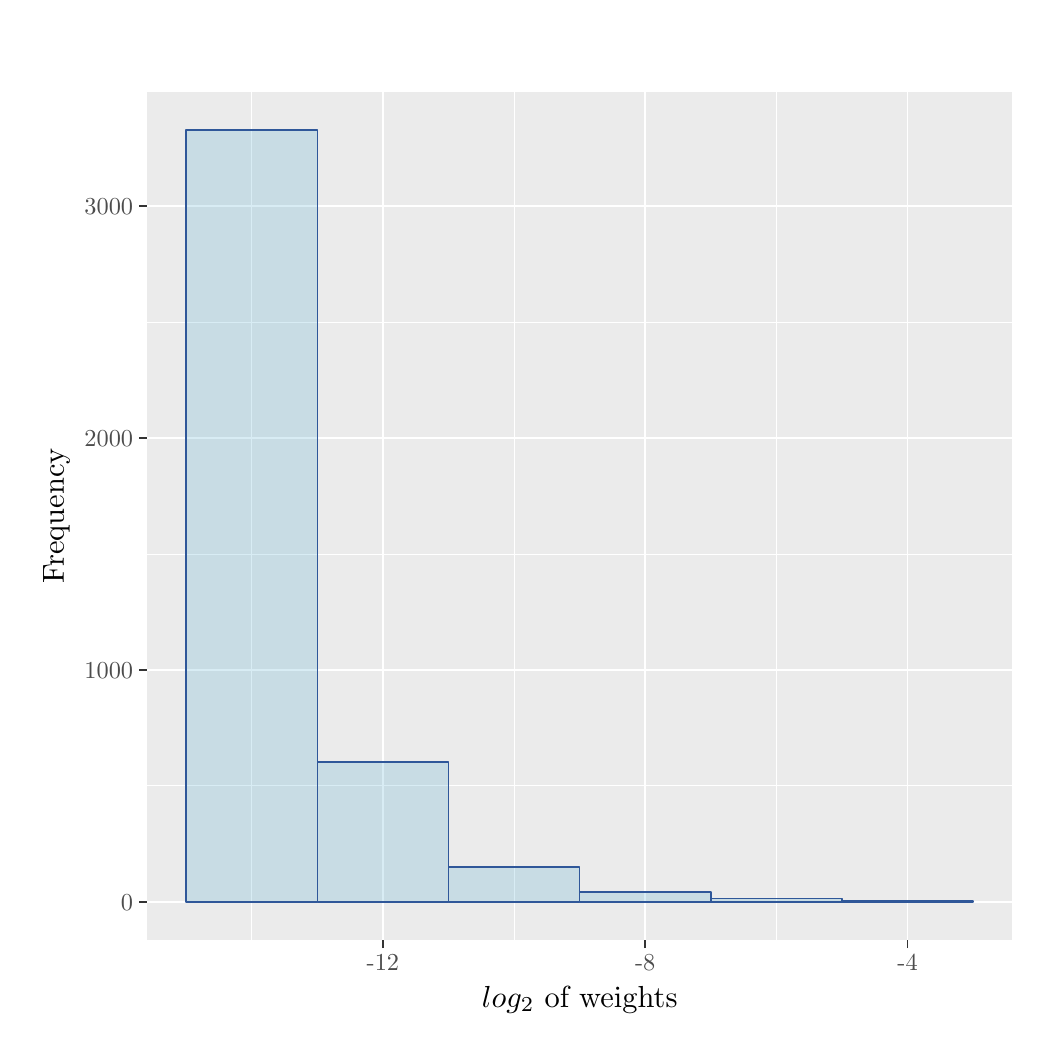
\begin{tikzpicture}[x=1pt,y=1pt]
\definecolor{fillColor}{RGB}{255,255,255}
\path[use as bounding box,fill=fillColor,fill opacity=0.00] (0,0) rectangle (361.35,361.35);
\begin{scope}
\path[clip] (  0.00,  0.00) rectangle (361.35,361.35);
\definecolor{drawColor}{RGB}{255,255,255}
\definecolor{fillColor}{RGB}{255,255,255}

\path[draw=drawColor,line width= 0.6pt,line join=round,line cap=round,fill=fillColor] (  0.00,  0.00) rectangle (361.35,361.35);
\end{scope}
\begin{scope}
\path[clip] ( 43.07, 31.53) rectangle (355.85,338.21);
\definecolor{fillColor}{gray}{0.92}

\path[fill=fillColor] ( 43.07, 31.53) rectangle (355.85,338.21);
\definecolor{drawColor}{RGB}{255,255,255}

\path[draw=drawColor,line width= 0.3pt,line join=round] ( 43.07, 87.37) --
	(355.85, 87.37);

\path[draw=drawColor,line width= 0.3pt,line join=round] ( 43.07,171.17) --
	(355.85,171.17);

\path[draw=drawColor,line width= 0.3pt,line join=round] ( 43.07,254.97) --
	(355.85,254.97);

\path[draw=drawColor,line width= 0.3pt,line join=round] ( 80.98, 31.53) --
	( 80.98,338.21);

\path[draw=drawColor,line width= 0.3pt,line join=round] (175.76, 31.53) --
	(175.76,338.21);

\path[draw=drawColor,line width= 0.3pt,line join=round] (270.55, 31.53) --
	(270.55,338.21);

\path[draw=drawColor,line width= 0.6pt,line join=round] ( 43.07, 45.47) --
	(355.85, 45.47);

\path[draw=drawColor,line width= 0.6pt,line join=round] ( 43.07,129.27) --
	(355.85,129.27);

\path[draw=drawColor,line width= 0.6pt,line join=round] ( 43.07,213.07) --
	(355.85,213.07);

\path[draw=drawColor,line width= 0.6pt,line join=round] ( 43.07,296.87) --
	(355.85,296.87);

\path[draw=drawColor,line width= 0.6pt,line join=round] (128.37, 31.53) --
	(128.37,338.21);

\path[draw=drawColor,line width= 0.6pt,line join=round] (223.15, 31.53) --
	(223.15,338.21);

\path[draw=drawColor,line width= 0.6pt,line join=round] (317.94, 31.53) --
	(317.94,338.21);
\definecolor{drawColor}{RGB}{47,87,153}
\definecolor{fillColor}{RGB}{62,164,201}

\path[draw=drawColor,line width= 0.6pt,line join=round,fill=fillColor,fill opacity=0.20] ( 57.28, 45.47) rectangle (104.67,324.27);

\path[draw=drawColor,line width= 0.6pt,line join=round,fill=fillColor,fill opacity=0.20] (104.67, 45.47) rectangle (152.07, 95.92);

\path[draw=drawColor,line width= 0.6pt,line join=round,fill=fillColor,fill opacity=0.20] (152.07, 45.47) rectangle (199.46, 58.12);

\path[draw=drawColor,line width= 0.6pt,line join=round,fill=fillColor,fill opacity=0.20] (199.46, 45.47) rectangle (246.85, 48.99);

\path[draw=drawColor,line width= 0.6pt,line join=round,fill=fillColor,fill opacity=0.20] (246.85, 45.47) rectangle (294.24, 46.64);

\path[draw=drawColor,line width= 0.6pt,line join=round,fill=fillColor,fill opacity=0.20] (294.24, 45.47) rectangle (341.63, 45.81);
\end{scope}
\begin{scope}
\path[clip] (  0.00,  0.00) rectangle (361.35,361.35);
\definecolor{drawColor}{gray}{0.30}

\node[text=drawColor,anchor=base east,inner sep=0pt, outer sep=0pt, scale=  0.88] at ( 38.12, 42.44) {0};

\node[text=drawColor,anchor=base east,inner sep=0pt, outer sep=0pt, scale=  0.88] at ( 38.12,126.24) {1000};

\node[text=drawColor,anchor=base east,inner sep=0pt, outer sep=0pt, scale=  0.88] at ( 38.12,210.04) {2000};

\node[text=drawColor,anchor=base east,inner sep=0pt, outer sep=0pt, scale=  0.88] at ( 38.12,293.84) {3000};
\end{scope}
\begin{scope}
\path[clip] (  0.00,  0.00) rectangle (361.35,361.35);
\definecolor{drawColor}{gray}{0.20}

\path[draw=drawColor,line width= 0.6pt,line join=round] ( 40.32, 45.47) --
	( 43.07, 45.47);

\path[draw=drawColor,line width= 0.6pt,line join=round] ( 40.32,129.27) --
	( 43.07,129.27);

\path[draw=drawColor,line width= 0.6pt,line join=round] ( 40.32,213.07) --
	( 43.07,213.07);

\path[draw=drawColor,line width= 0.6pt,line join=round] ( 40.32,296.87) --
	( 43.07,296.87);
\end{scope}
\begin{scope}
\path[clip] (  0.00,  0.00) rectangle (361.35,361.35);
\definecolor{drawColor}{gray}{0.20}

\path[draw=drawColor,line width= 0.6pt,line join=round] (128.37, 28.78) --
	(128.37, 31.53);

\path[draw=drawColor,line width= 0.6pt,line join=round] (223.15, 28.78) --
	(223.15, 31.53);

\path[draw=drawColor,line width= 0.6pt,line join=round] (317.94, 28.78) --
	(317.94, 31.53);
\end{scope}
\begin{scope}
\path[clip] (  0.00,  0.00) rectangle (361.35,361.35);
\definecolor{drawColor}{gray}{0.30}

\node[text=drawColor,anchor=base,inner sep=0pt, outer sep=0pt, scale=  0.88] at (128.37, 20.52) {-12};

\node[text=drawColor,anchor=base,inner sep=0pt, outer sep=0pt, scale=  0.88] at (223.15, 20.52) {-8};

\node[text=drawColor,anchor=base,inner sep=0pt, outer sep=0pt, scale=  0.88] at (317.94, 20.52) {-4};
\end{scope}
\begin{scope}
\path[clip] (  0.00,  0.00) rectangle (361.35,361.35);
\definecolor{drawColor}{RGB}{0,0,0}

\node[text=drawColor,anchor=base,inner sep=0pt, outer sep=0pt, scale=  1.10] at (199.46,  7.44) {$log_2$ of weights};
\end{scope}
\begin{scope}
\path[clip] (  0.00,  0.00) rectangle (361.35,361.35);
\definecolor{drawColor}{RGB}{0,0,0}

\node[text=drawColor,rotate= 90.00,anchor=base,inner sep=0pt, outer sep=0pt, scale=  1.10] at ( 13.08,184.87) {Frequency};
\end{scope}
\begin{scope}
\path[clip] (  0.00,  0.00) rectangle (361.35,361.35);
\definecolor{drawColor}{RGB}{0,0,0}


\end{scope}
\end{tikzpicture}


%}
%\caption{Distribution of the weights after normalization.}
%\label{fig:norm}
%\end{figure}

%even though the $log$ of weights will normalize them between $-1$ and  $-14$ (illustrated in Figure~\ref{fig:norm}), 
\noindent
\emph{Normalization:} Some variations to the model were experimented with but because of extremely poor results were disregard. One of such approaches was normalization. In an attempt to boost performance, weights of the graph were normalized using log normalization. We chose a \emph{$log$ normalization}, in order to reduce the range of values, in which the weights fluctuate. Moreover, the gradient descent algorithm can converge more smoothly to the functions minimum. Unfortunately, adding the normalization made the problem ill-conditioned and the algorithm could not converge to a solution and was dismissed early on. The reason for this could be that in the cost function a second $log$ is applied to the inputs. Because the normalization $log$ might result into negative values and the $log$ of a negative number is undefined it results in undefined gradient updates and untrainable weights. Other than log normalization, linear transformation like \emph{min max normalization} were also experimented. Min max normalization will force all the weights to be between $0$ and $1$ and is calculated with Equation~\ref{eq:minmaxNom}, where $e=(e_1,...,e_n)$ is the set of input weights and $z_i$ is the $i$th normalized data. Unfortunately, adding this form of normalization did not improve the results and are also removed from the model.
\begin{equation}
z_{ i }=\frac { e_{ i }-min(e) }{ max(e)-min(e) } 
\label{eq:minmaxNom}
\end{equation}
\noindent
\emph{Adding $1$ to the $log$:} The cost function applies logarithm to the weights. For edge weight of $1$ the $log(1)=0$. Therefore, we tested the model with the addition of $1$ to the $log$ of weights, to adjust for this effect. With this change, the cost function is changed to Equation~\ref{eq:log_plus}. Although in some cases this change improved the model performance, in other cases it generated poor results. More details about how this change effects the model is discussed in Section~\ref{sec:setup}. 
\begin{equation}
J_e=\sum _{ j=1 }^{ V }{}\sum _{ i=1 }^{ V_e }{ f({ X }_{ ij } } )(w_{ i }^{ T }\tilde{  w_{ j } } +b_{ i }+\tilde{  b_{ j } } -(log{ X }_{ ij }+1))^2
\label{eq:log_plus}
\end{equation}
\begin{figure}
{\small 
\tikzset{every picture/.style={line width=0.75pt}} %set default line width to 0.75pt        

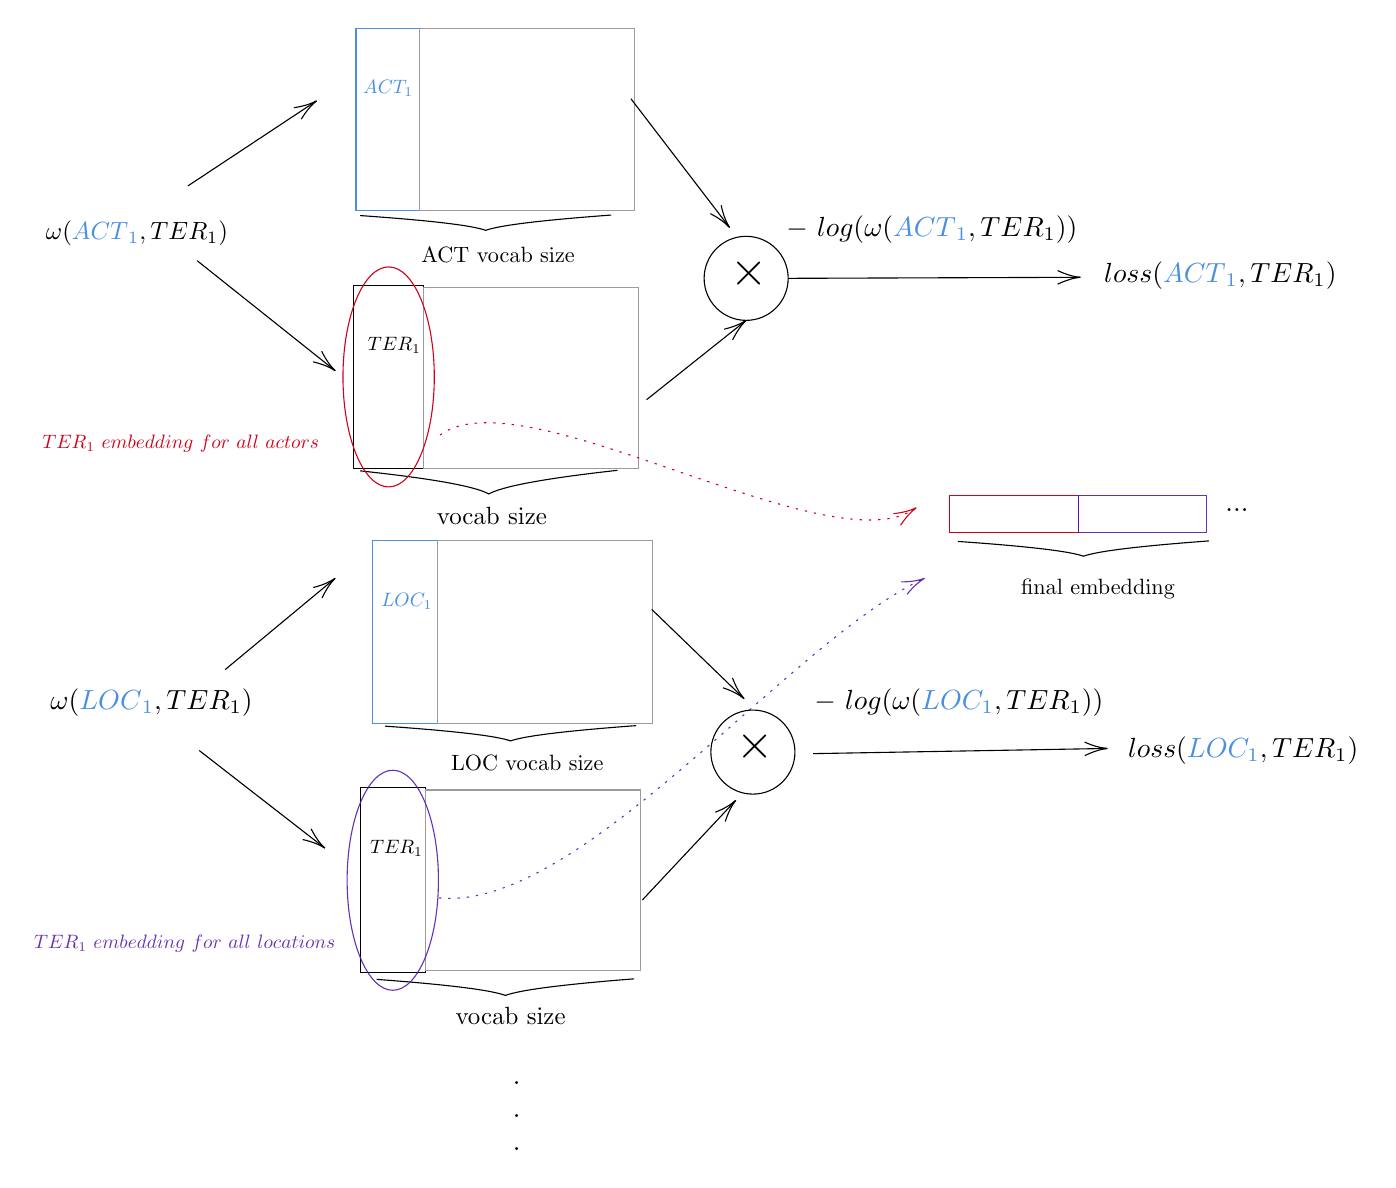
\begin{tikzpicture}[x=0.75pt,y=0.75pt,yscale=-1,xscale=1]
%uncomment if require: \path (0,573); %set diagram left start at 0, and has height of 573

\draw    (373.75,127.5) -- (514.5,127) ;
\draw [shift={(514.5,127)}, rotate = 539.8] [color={rgb, 255:red, 0; green, 0; blue, 0 }  ]   (0,0) .. controls (3.31,-0.3) and (6.95,-1.4) .. (10.93,-3.29)(0,0) .. controls (3.31,0.3) and (6.95,1.4) .. (10.93,3.29)   ;

\draw    (84.5,83) -- (146.5,42) ;
\draw [shift={(146.5,42)}, rotate = 506.52] [color={rgb, 255:red, 0; green, 0; blue, 0 }  ]   (0,0) .. controls (3.31,-0.3) and (6.95,-1.4) .. (10.93,-3.29)(0,0) .. controls (3.31,0.3) and (6.95,1.4) .. (10.93,3.29)   ;

\draw  [color={rgb, 255:red, 74; green, 144; blue, 226 }  ,draw opacity=1 ]  (165.5, 7) rectangle (196, 95)   ;
\draw    (164.5, 131) rectangle (198, 219)   ;
\draw  [color={rgb, 255:red, 155; green, 155; blue, 155 }  ,draw opacity=1 ]  (196, 7) rectangle (299.5, 95)   ;
\draw  [color={rgb, 255:red, 155; green, 155; blue, 155 }  ,draw opacity=1 ]  (198, 132) rectangle (301.5, 219)   ;
\draw [rotate around= { 89.88: (229.51, 225.75)
    }]  (223.89,163.75) .. controls (227.64,198.19) and (231.38,218.86) .. (235.13,225.75) .. controls (231.38,232.64) and (227.64,253.31) .. (223.89,287.75) ;
\draw [rotate around= { 89.88: (228.01, 100.75)
    }]  (224.39,40.25) .. controls (226.8,73.86) and (229.22,94.03) .. (231.63,100.75) .. controls (229.22,107.47) and (226.8,127.64) .. (224.39,161.25) ;
\draw    (353.5, 127.5) circle [x radius= 20.25, y radius= 20.25]  ;
\draw    (305.5,186) -- (353.5,147.75) ;
\draw [shift={(353.5,147.75)}, rotate = 501.45] [color={rgb, 255:red, 0; green, 0; blue, 0 }  ]   (0,0) .. controls (3.31,-0.3) and (6.95,-1.4) .. (10.93,-3.29)(0,0) .. controls (3.31,0.3) and (6.95,1.4) .. (10.93,3.29)   ;

\draw    (298,41) -- (345.5,103) ;
\draw [shift={(345.5,103)}, rotate = 232.54] [color={rgb, 255:red, 0; green, 0; blue, 0 }  ]   (0,0) .. controls (3.31,-0.3) and (6.95,-1.4) .. (10.93,-3.29)(0,0) .. controls (3.31,0.3) and (6.95,1.4) .. (10.93,3.29)   ;

\draw    (90,355) -- (150.5,402) ;
\draw [shift={(150.5,402)}, rotate = 217.84] [color={rgb, 255:red, 0; green, 0; blue, 0 }  ]   (0,0) .. controls (3.31,-0.3) and (6.95,-1.4) .. (10.93,-3.29)(0,0) .. controls (3.31,0.3) and (6.95,1.4) .. (10.93,3.29)   ;

\draw    (102.5,316) -- (155.5,272) ;
\draw [shift={(155.5,272)}, rotate = 500.3] [color={rgb, 255:red, 0; green, 0; blue, 0 }  ]   (0,0) .. controls (3.31,-0.3) and (6.95,-1.4) .. (10.93,-3.29)(0,0) .. controls (3.31,0.3) and (6.95,1.4) .. (10.93,3.29)   ;

\draw  [color={rgb, 255:red, 74; green, 144; blue, 226 }  ,draw opacity=1 ]  (173.5, 254) rectangle (205, 342)   ;
\draw    (167.5, 373) rectangle (199, 462)   ;
\draw  [color={rgb, 255:red, 155; green, 155; blue, 155 }  ,draw opacity=1 ]  (205, 254) rectangle (308.5, 342)   ;
\draw  [color={rgb, 255:red, 155; green, 155; blue, 155 }  ,draw opacity=1 ]  (199, 374) rectangle (302.5, 461)   ;
\draw [rotate around= { 89.88: (237.51, 469.07)
    }]  (233.57,407.07) .. controls (236.2,441.51) and (238.82,462.18) .. (241.44,469.07) .. controls (238.82,475.95) and (236.2,496.62) .. (233.57,531.07) ;
\draw    (356.75, 355.75) circle [x radius= 20.25, y radius= 20.25]  ;
\draw    (303.5,427) -- (348.5,379) ;
\draw [shift={(348.5,379)}, rotate = 493.15] [color={rgb, 255:red, 0; green, 0; blue, 0 }  ]   (0,0) .. controls (3.31,-0.3) and (6.95,-1.4) .. (10.93,-3.29)(0,0) .. controls (3.31,0.3) and (6.95,1.4) .. (10.93,3.29)   ;

\draw    (308,287) -- (352.5,330) ;
\draw [shift={(352.5,330)}, rotate = 224.02] [color={rgb, 255:red, 0; green, 0; blue, 0 }  ]   (0,0) .. controls (3.31,-0.3) and (6.95,-1.4) .. (10.93,-3.29)(0,0) .. controls (3.31,0.3) and (6.95,1.4) .. (10.93,3.29)   ;

\draw [rotate around= { 89.88: (240.01, 346.75)
    }]  (236.39,286.25) .. controls (238.8,319.86) and (241.22,340.03) .. (243.63,346.75) .. controls (241.22,353.47) and (238.8,373.64) .. (236.39,407.25) ;
\draw  [color={rgb, 255:red, 208; green, 2; blue, 27 }  ,draw opacity=1 ]  (181.25, 175) circle [x radius= 22, y radius= 53]  ;
\draw  [color={rgb, 255:red, 82; green, 21; blue, 168 }  ,draw opacity=0.88 ]  (183.25, 417.5) circle [x radius= 22, y radius= 53]  ;
\draw [color={rgb, 255:red, 208; green, 2; blue, 27 }  ,draw opacity=1 ] [dash pattern={on 0.84pt off 2.51pt}]  (206,203) .. controls (246,173) and (395.5,268) .. (435.5,238) ;
\draw [shift={(435.5,238)}, rotate = 508.65] [color={rgb, 255:red, 208; green, 2; blue, 27 }  ,draw opacity=1 ]   (0,0) .. controls (3.31,-0.3) and (6.95,-1.4) .. (10.93,-3.29)(0,0) .. controls (3.31,0.3) and (6.95,1.4) .. (10.93,3.29)   ;

\draw [color={rgb, 255:red, 82; green, 21; blue, 168 }  ,draw opacity=0.88 ] [dash pattern={on 0.84pt off 2.51pt}]  (205.5,426) .. controls (273.5,433) and (375.5,301) .. (439.5,272) ;
\draw [shift={(439.5,272)}, rotate = 514.4] [color={rgb, 255:red, 82; green, 21; blue, 168 }  ,draw opacity=0.88 ]   (0,0) .. controls (3.31,-0.3) and (6.95,-1.4) .. (10.93,-3.29)(0,0) .. controls (3.31,0.3) and (6.95,1.4) .. (10.93,3.29)   ;

\draw  [color={rgb, 255:red, 208; green, 2; blue, 27 }  ,draw opacity=1 ]  (451.5, 232) rectangle (513.5, 250)   ;
\draw  [color={rgb, 255:red, 82; green, 21; blue, 168 }  ,draw opacity=0.88 ]  (513.5, 232) rectangle (575.5, 250)   ;
\draw    (89,119) -- (155.5,172) ;
\draw [shift={(155.5,172)}, rotate = 218.55] [color={rgb, 255:red, 0; green, 0; blue, 0 }  ]   (0,0) .. controls (3.31,-0.3) and (6.95,-1.4) .. (10.93,-3.29)(0,0) .. controls (3.31,0.3) and (6.95,1.4) .. (10.93,3.29)   ;

\draw    (385.75,356.5) -- (527.5,354) ;
\draw [shift={(527.5,354)}, rotate = 538.99] [color={rgb, 255:red, 0; green, 0; blue, 0 }  ]   (0,0) .. controls (3.31,-0.3) and (6.95,-1.4) .. (10.93,-3.29)(0,0) .. controls (3.31,0.3) and (6.95,1.4) .. (10.93,3.29)   ;

\draw [rotate around= { 89.88: (516.01, 257.75)
    }]  (512.39,197.25) .. controls (514.8,230.86) and (517.22,251.03) .. (519.63,257.75) .. controls (517.22,264.47) and (514.8,284.64) .. (512.39,318.25) ;

\draw (60,106) node [scale=0.9] [align=left] {$\omega (\textcolor[rgb]{0.29,0.56,0.89}{ACT}\textcolor[rgb]{0.29,0.56,0.89}{_{1}} ,TER_{1})$};
\draw (181,36) node [scale=0.7,color={rgb, 255:red, 74; green, 144; blue, 226 }  ,opacity=1 ]  {$ACT_{1}$};
\draw (582,126) node  [align=left] {$loss(\textcolor[rgb]{0.29,0.56,0.89}{ACT}\textcolor[rgb]{0.29,0.56,0.89}{_{1}} ,TER_{1})$};
\draw (184,160) node [scale=0.7]  {$TER_{1}$};
\draw (234,116) node [scale=0.8] [align=left] {ACT vocab size};
\draw (231,242) node [scale=0.9] [align=left] {vocab size};
\draw (67,332) node  [align=left] {$\omega (\textcolor[rgb]{0.29,0.56,0.89}{LOC}\textcolor[rgb]{0.29,0.56,0.89}{_{1}} ,TER_{1})$};
\draw (190,283) node [scale=0.7,color={rgb, 255:red, 74; green, 144; blue, 226 }  ,opacity=1 ]  {$LOC_{1}$};
\draw (185,402) node [scale=0.7]  {$TER_{1}$};
\draw (248,361) node [scale=0.8] [align=left] {LOC vocab size};
\draw (240,483) node [scale=0.9] [align=left] {vocab size};
\draw (243,531) node  [align=left] {.\\.\\.};
\draw (81,207) node [scale=0.7,color={rgb, 255:red, 208; green, 2; blue, 27 }  ,opacity=1 ]  {$TER_{1} \ embedding\ for\ all\ actors$};
\draw (83,448) node [scale=0.7,color={rgb, 255:red, 82; green, 21; blue, 168 }  ,opacity=0.88 ]  {$TER_{1} \ embedding\ for\ all\ locations$};
\draw (590,239) node  [align=left] {...};
\draw (443,104) node  [align=left] {$-\ log( \omega (\textcolor[rgb]{0.29,0.56,0.89}{ACT}\textcolor[rgb]{0.29,0.56,0.89}{_{1}} ,TER_{1}))$};
\draw (593,355) node  [align=left] {$loss(\textcolor[rgb]{0.29,0.56,0.89}{LOC_{1}} ,TER_{1})$};
\draw (456,332) node  [align=left] {$-\ log( \omega (\textcolor[rgb]{0.29,0.56,0.89}{LOC_{1}} ,TER_{1}))$};
\draw (523,277) node [scale=0.8] [align=left] {final embedding};
\draw (355,125) node [scale=1.7280000000000002]  {$\times $};
\draw (358,353) node [scale=1.7280000000000002]  {$\times $};

\end{tikzpicture}



}
\caption{Facetted embedding with separate cost functions. Contains traning of five different networks (two are shown in the figure) for a single input. The target word is \emph{TER1}, which is being tranined against all actors, organisations, locations, dates and terms. The final embedding is created by concatinating the columns in the context embedding matricies that are acossiated with \emph{TER1}.   } \label{fig:separate_cost}
\end{figure}
\begin{figure}
{\small 
\tikzset{every picture/.style={line width=0.75pt}} %set default line width to 0.75pt   

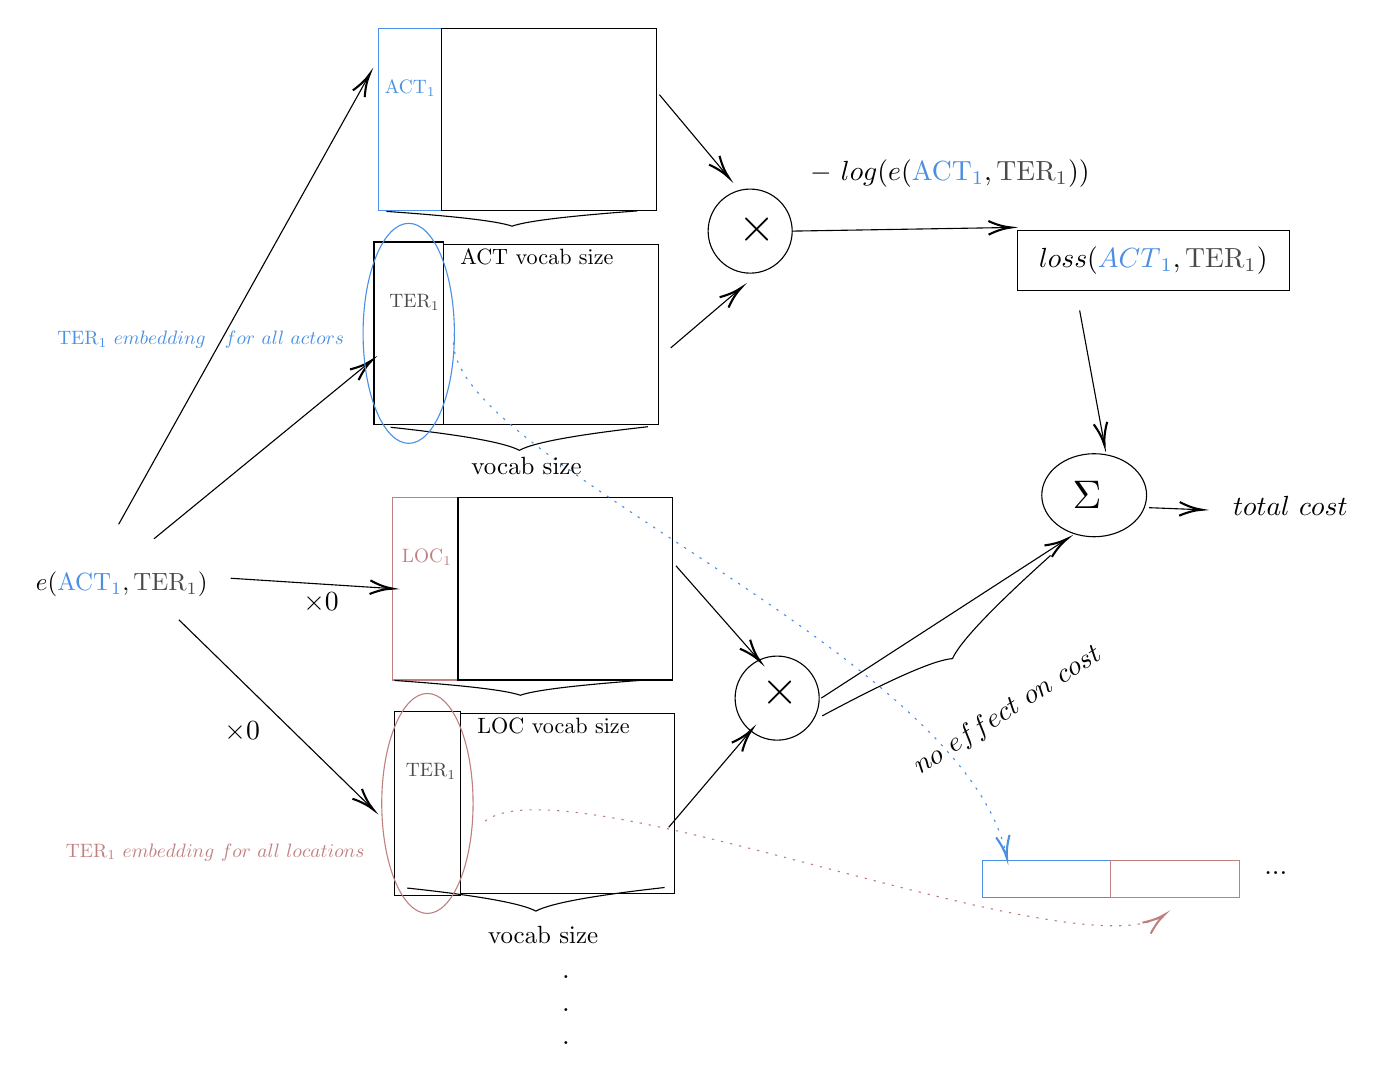
\begin{tikzpicture}[x=0.75pt,y=0.75pt,yscale=-1,xscale=1]
%uncomment if require: \path (0,547); %set diagram left start at 0, and has height of 547

%Straight Lines [id:da13430096728319052] 
\draw    (71.5,277) -- (174.95,192.27) ;
\draw [shift={(176.5,191)}, rotate = 500.68] [color={rgb, 255:red, 0; green, 0; blue, 0 }  ][line width=0.75]    (10.93,-3.29) .. controls (6.95,-1.4) and (3.31,-0.3) .. (0,0) .. controls (3.31,0.3) and (6.95,1.4) .. (10.93,3.29)   ;

%Straight Lines [id:da3395203365138022] 
\draw    (54.5,270) -- (174.53,54.75) ;
\draw [shift={(175.5,53)}, rotate = 479.14] [color={rgb, 255:red, 0; green, 0; blue, 0 }  ][line width=0.75]    (10.93,-3.29) .. controls (6.95,-1.4) and (3.31,-0.3) .. (0,0) .. controls (3.31,0.3) and (6.95,1.4) .. (10.93,3.29)   ;

%Shape: Rectangle [id:dp40988752111198234] 
\draw  [color={rgb, 255:red, 74; green, 144; blue, 226 }  ,draw opacity=1 ] (179.5,31) -- (210,31) -- (210,119) -- (179.5,119) -- cycle ;
%Shape: Rectangle [id:dp8120457242640955] 
\draw   (177.5,134) -- (211,134) -- (211,222) -- (177.5,222) -- cycle ;
%Shape: Rectangle [id:dp5994549314957651] 
\draw  [color={rgb, 255:red, 0; green, 0; blue, 0 }  ,draw opacity=1 ] (210,31) -- (313.5,31) -- (313.5,119) -- (210,119) -- cycle ;
%Shape: Rectangle [id:dp8953379233256253] 
\draw  [color={rgb, 255:red, 0; green, 0; blue, 0 }  ,draw opacity=1 ] (211,135) -- (314.5,135) -- (314.5,222) -- (211,222) -- cycle ;
\draw   (309.5,223) .. controls (275.06,226.82) and (254.4,230.61) .. (247.52,234.37) .. controls (240.63,230.64) and (219.95,226.93) .. (185.5,223.26) ;
\draw   (304.5,119) .. controls (270.9,121.49) and (250.73,123.94) .. (244.02,126.37) .. controls (237.29,123.97) and (217.12,121.6) .. (183.5,119.25) ;
%Shape: Ellipse [id:dp16021666171497673] 
\draw   (338.5,128.75) .. controls (338.5,117.57) and (347.57,108.5) .. (358.75,108.5) .. controls (369.93,108.5) and (379,117.57) .. (379,128.75) .. controls (379,139.93) and (369.93,149) .. (358.75,149) .. controls (347.57,149) and (338.5,139.93) .. (338.5,128.75) -- cycle ;
%Straight Lines [id:da010832594540308715] 
\draw    (320.5,185) -- (352.98,157.3) ;
\draw [shift={(354.5,156)}, rotate = 499.54] [color={rgb, 255:red, 0; green, 0; blue, 0 }  ][line width=0.75]    (10.93,-3.29) .. controls (6.95,-1.4) and (3.31,-0.3) .. (0,0) .. controls (3.31,0.3) and (6.95,1.4) .. (10.93,3.29)   ;

%Straight Lines [id:da7904695547993323] 
\draw    (315,63) -- (347.22,101.47) ;
\draw [shift={(348.5,103)}, rotate = 230.05] [color={rgb, 255:red, 0; green, 0; blue, 0 }  ][line width=0.75]    (10.93,-3.29) .. controls (6.95,-1.4) and (3.31,-0.3) .. (0,0) .. controls (3.31,0.3) and (6.95,1.4) .. (10.93,3.29)   ;

%Straight Lines [id:da40310566362864897] 
\draw    (517.5,167) -- (529.14,230.03) ;
\draw [shift={(529.5,232)}, rotate = 259.54] [color={rgb, 255:red, 0; green, 0; blue, 0 }  ][line width=0.75]    (10.93,-3.29) .. controls (6.95,-1.4) and (3.31,-0.3) .. (0,0) .. controls (3.31,0.3) and (6.95,1.4) .. (10.93,3.29)   ;

%Shape: Rectangle [id:dp7172146507008619] 
\draw  [color={rgb, 255:red, 191; green, 128; blue, 128 }  ,draw opacity=1 ] (186.5,257) -- (218,257) -- (218,345) -- (186.5,345) -- cycle ;
%Shape: Rectangle [id:dp060267406747659624] 
\draw   (187.5,360) -- (219,360) -- (219,449) -- (187.5,449) -- cycle ;
%Shape: Rectangle [id:dp6303673802072765] 
\draw  [color={rgb, 255:red, 0; green, 0; blue, 0 }  ,draw opacity=1 ] (218,257) -- (321.5,257) -- (321.5,345) -- (218,345) -- cycle ;
%Shape: Rectangle [id:dp304301296261714] 
\draw  [color={rgb, 255:red, 0; green, 0; blue, 0 }  ,draw opacity=1 ] (219,361) -- (322.5,361) -- (322.5,448) -- (219,448) -- cycle ;
\draw   (317.5,445) .. controls (283.06,448.82) and (262.4,452.61) .. (255.52,456.37) .. controls (248.63,452.64) and (227.95,448.93) .. (193.5,445.26) ;
%Shape: Ellipse [id:dp22428072345396544] 
\draw   (351.5,353.75) .. controls (351.5,342.57) and (360.57,333.5) .. (371.75,333.5) .. controls (382.93,333.5) and (392,342.57) .. (392,353.75) .. controls (392,364.93) and (382.93,374) .. (371.75,374) .. controls (360.57,374) and (351.5,364.93) .. (351.5,353.75) -- cycle ;
%Straight Lines [id:da29040700011246456] 
\draw    (319.5,416) -- (358.2,370.52) ;
\draw [shift={(359.5,369)}, rotate = 490.4] [color={rgb, 255:red, 0; green, 0; blue, 0 }  ][line width=0.75]    (10.93,-3.29) .. controls (6.95,-1.4) and (3.31,-0.3) .. (0,0) .. controls (3.31,0.3) and (6.95,1.4) .. (10.93,3.29)   ;

%Straight Lines [id:da7545042977801857] 
\draw    (323,290) -- (362.18,334.5) ;
\draw [shift={(363.5,336)}, rotate = 228.64] [color={rgb, 255:red, 0; green, 0; blue, 0 }  ][line width=0.75]    (10.93,-3.29) .. controls (6.95,-1.4) and (3.31,-0.3) .. (0,0) .. controls (3.31,0.3) and (6.95,1.4) .. (10.93,3.29)   ;

%Straight Lines [id:da13418076605656504] 
\draw    (393,353.75) -- (509.82,278.09) ;
\draw [shift={(511.5,277)}, rotate = 507.07] [color={rgb, 255:red, 0; green, 0; blue, 0 }  ][line width=0.75]    (10.93,-3.29) .. controls (6.95,-1.4) and (3.31,-0.3) .. (0,0) .. controls (3.31,0.3) and (6.95,1.4) .. (10.93,3.29)   ;

\draw   (308.5,345) .. controls (274.9,347.49) and (254.73,349.94) .. (248.02,352.37) .. controls (241.29,349.97) and (221.12,347.6) .. (187.5,345.25) ;
%Shape: Ellipse [id:dp1891084828946663] 
\draw  [color={rgb, 255:red, 74; green, 144; blue, 226 }  ,draw opacity=1 ] (172.25,178) .. controls (172.25,148.73) and (182.1,125) .. (194.25,125) .. controls (206.4,125) and (216.25,148.73) .. (216.25,178) .. controls (216.25,207.27) and (206.4,231) .. (194.25,231) .. controls (182.1,231) and (172.25,207.27) .. (172.25,178) -- cycle ;
%Shape: Ellipse [id:dp5133297466247488] 
\draw  [color={rgb, 255:red, 191; green, 128; blue, 128 }  ,draw opacity=1 ] (181.25,404.5) .. controls (181.25,375.23) and (191.1,351.5) .. (203.25,351.5) .. controls (215.4,351.5) and (225.25,375.23) .. (225.25,404.5) .. controls (225.25,433.77) and (215.4,457.5) .. (203.25,457.5) .. controls (191.1,457.5) and (181.25,433.77) .. (181.25,404.5) -- cycle ;
%Shape: Rectangle [id:dp8154703521346762] 
\draw  [color={rgb, 255:red, 74; green, 144; blue, 226 }  ,draw opacity=1 ] (470.5,432) -- (532.5,432) -- (532.5,450) -- (470.5,450) -- cycle ;
%Shape: Rectangle [id:dp3576905019222951] 
\draw  [color={rgb, 255:red, 191; green, 128; blue, 128 }  ,draw opacity=1 ] (532.5,432) -- (594.5,432) -- (594.5,450) -- (532.5,450) -- cycle ;
%Straight Lines [id:da3207889104512305] 
\draw    (108.5,296) -- (184.5,300.87) ;
\draw [shift={(186.5,301)}, rotate = 183.67] [color={rgb, 255:red, 0; green, 0; blue, 0 }  ][line width=0.75]    (10.93,-3.29) .. controls (6.95,-1.4) and (3.31,-0.3) .. (0,0) .. controls (3.31,0.3) and (6.95,1.4) .. (10.93,3.29)   ;

%Straight Lines [id:da444746435738554] 
\draw    (83.5,316) -- (175.82,406.1) ;
\draw [shift={(177.25,407.5)}, rotate = 224.3] [color={rgb, 255:red, 0; green, 0; blue, 0 }  ][line width=0.75]    (10.93,-3.29) .. controls (6.95,-1.4) and (3.31,-0.3) .. (0,0) .. controls (3.31,0.3) and (6.95,1.4) .. (10.93,3.29)   ;

\draw   (503.5,285) .. controls (475.52,310.16) and (459.77,326.73) .. (456.25,334.71) .. controls (447.55,335.32) and (426.62,344.52) .. (393.47,362.3) ;
%Shape: Ellipse [id:dp6408782289262511] 
\draw   (499.25,256) .. controls (499.25,244.95) and (510.55,236) .. (524.5,236) .. controls (538.45,236) and (549.75,244.95) .. (549.75,256) .. controls (549.75,267.05) and (538.45,276) .. (524.5,276) .. controls (510.55,276) and (499.25,267.05) .. (499.25,256) -- cycle ;
%Straight Lines [id:da19133214528940812] 
\draw    (379,128.75) -- (482.5,127.03) ;
\draw [shift={(484.5,127)}, rotate = 539.05] [color={rgb, 255:red, 0; green, 0; blue, 0 }  ][line width=0.75]    (10.93,-3.29) .. controls (6.95,-1.4) and (3.31,-0.3) .. (0,0) .. controls (3.31,0.3) and (6.95,1.4) .. (10.93,3.29)   ;

%Straight Lines [id:da406862365844594] 
\draw    (551,262) -- (574.5,262.92) ;
\draw [shift={(576.5,263)}, rotate = 182.25] [color={rgb, 255:red, 0; green, 0; blue, 0 }  ][line width=0.75]    (10.93,-3.29) .. controls (6.95,-1.4) and (3.31,-0.3) .. (0,0) .. controls (3.31,0.3) and (6.95,1.4) .. (10.93,3.29)   ;

%Curve Lines [id:da14396608756415818] 
\draw [color={rgb, 255:red, 191; green, 128; blue, 128 }  ,draw opacity=1 ] [dash pattern={on 0.84pt off 2.51pt}]  (231,413) .. controls (270.6,383.3) and (513.57,485.91) .. (557.24,458.86) ;
\draw [shift={(558.5,458)}, rotate = 503.13] [color={rgb, 255:red, 191; green, 128; blue, 128 }  ,draw opacity=1 ][line width=0.75]    (10.93,-3.29) .. controls (6.95,-1.4) and (3.31,-0.3) .. (0,0) .. controls (3.31,0.3) and (6.95,1.4) .. (10.93,3.29)   ;

%Curve Lines [id:da8005082280810756] 
\draw [color={rgb, 255:red, 74; green, 144; blue, 226 }  ,draw opacity=1 ] [dash pattern={on 0.84pt off 2.51pt}]  (216.25,178) .. controls (203.56,234.72) and (460.91,329.05) .. (482.2,429.49) ;
\draw [shift={(482.5,431)}, rotate = 259.35] [color={rgb, 255:red, 74; green, 144; blue, 226 }  ,draw opacity=1 ][line width=0.75]    (10.93,-3.29) .. controls (6.95,-1.4) and (3.31,-0.3) .. (0,0) .. controls (3.31,0.3) and (6.95,1.4) .. (10.93,3.29)   ;


% Text Node
\draw (195,60) node [scale=0.7,color={rgb, 255:red, 74; green, 144; blue, 226 }  ,opacity=1 ]  {$\mathrm{ACT}_{1}$};
% Text Node
\draw (362,128) node [scale=1.7280000000000002]  {$\times $};
% Text Node
\draw (197,163) node [scale=0.7,color={rgb, 255:red, 74; green, 74; blue, 74 }  ,opacity=1 ]  {$\mathrm{TER}_{1}$};
% Text Node
\draw (256,141) node [scale=0.8] [align=left] {ACT vocab size};
% Text Node
\draw (251,242) node [scale=0.9] [align=left] {vocab size};
% Text Node
\draw (203,286) node [scale=0.7,color={rgb, 255:red, 191; green, 128; blue, 128 }  ,opacity=1 ]  {$\mathrm{LOC}_{1}$};
% Text Node
\draw (205,389) node [scale=0.7,color={rgb, 255:red, 74; green, 74; blue, 74 }  ,opacity=1 ]  {$\mathrm{TER}_{1}$};
% Text Node
\draw (264,367) node [scale=0.8] [align=left] {LOC vocab size};
% Text Node
\draw (259,468) node [scale=0.9] [align=left] {vocab size};
% Text Node
\draw (270,504) node  [align=left] {.\\.\\.};
% Text Node
\draw (94,181) node [scale=0.7,color={rgb, 255:red, 74; green, 144; blue, 226 }  ,opacity=1 ]  {$\mathrm{TER}_{1} \ embedding\ \ \ for\ all\ actors$};
% Text Node
\draw (101,428) node [scale=0.7,color={rgb, 255:red, 191; green, 128; blue, 128 }  ,opacity=1 ]  {$\mathrm{TER}_{1} \ embedding\ for\ all\ locations$};
% Text Node
\draw (612,438) node  [align=left] {...};
% Text Node
\draw (114,370) node   {$\times 0$};
% Text Node
\draw (152,308) node   {$\times 0$};
% Text Node
\draw (483,360) node [rotate=-327.48]  {$ \begin{array}{l}
no\ effect\ on\ cost\\
\end{array}$};
% Text Node
\draw (521,256) node [scale=1.44]  {$\Sigma $};
% Text Node
\draw (373,351) node [scale=1.7280000000000002]  {$\times $};
% Text Node
\draw (56,299) node [scale=0.9] [align=left] {$e (\textcolor[rgb]{0.29,0.56,0.89}{\mathrm{ACT}}\textcolor[rgb]{0.29,0.56,0.89}{_{1}} ,\textcolor[rgb]{0.29,0.29,0.29}{\mathrm{TER}_{1}})$};
% Text Node
\draw    (487.5,128.5) -- (618.5,128.5) -- (618.5,157.5) -- (487.5,157.5) -- cycle  ;
\draw (553,143) node  [align=left] {$loss(\textcolor[rgb]{0.29,0.56,0.89}{ACT}\textcolor[rgb]{0.29,0.56,0.89}{_{1}} ,\textcolor[rgb]{0.29,0.29,0.29}{\mathrm{TER}_{1}})$};
% Text Node
\draw (455,101) node  [align=left] {$-\ log( e (\textcolor[rgb]{0.29,0.56,0.89}{\mathrm{ACT}}\textcolor[rgb]{0.29,0.56,0.89}{_{1}} ,\textcolor[rgb]{0.29,0.29,0.29}{\mathrm{TER}_{1}}))$};
% Text Node
\draw (619,261) node  [align=left] {$total\ cost$};


\end{tikzpicture}
\caption{Facetted embedding with unified cost function. Training for a single input is shown using only one network. The target word is \emph{TER1}, which is being tranined against all actors, organisations, locations, dates and terms. While training the weights related to actors are only updated if the input edge weight has the start node type of an actor. Meanwhile,the rest of the weights related to other entity-types are freezed. The final embedding is created by concatinating the columns in the context embedding matricies that are acossiated with \emph{TER1}.} \label{fig:unified_cost}
}
\end{figure}
\subsubsection{Unified cost function  }
\label{sec:unified_cost}
The unified cost function is simply the summation of all the separate cost functions in the previous section, where $E$ is the set of all possible types, shown in Equation~\ref{eq:unified_cost}.
\begin{equation}
J=\sum _{ e=1 }^{ E }{J_e}=\sum _{ e=1 }^{ E }{}\sum _{ j=1 }^{ V }{}\sum _{ i=1 }^{ V_e }{ f({ X }_{ ij } } )(w_{ i }^{ T }\tilde{  w_{ j } } +b_{ i }+\tilde{  b_{ j } } -log{ X }_{ ij })^2
\label{eq:unified_cost}
\end{equation}
As a result, all embeddings can be generated with a single network. For a better understanding of the differences between the methods a visual comparison is shown in Figures~\ref{fig:separate_cost} and~\ref{fig:unified_cost} for loss on a single input. Each input is an edge with its corresponding weight, if the input has the starting node of type actor, the rest of the layers related to other types of embeddings will be frozen during training and only the weights for the actor network will be updated through backpropagation. Hence, it is as if all the networks were trained separately, because the weights of a certain type can only be updated when the correct input is presented.  \\
In Figure~\ref{fig:separate_cost}, two of the five networks are shown as an example. A single edge refers to two embeddings, one for the focal (start node) and one for the context (end node). Each network is trained separately and a final embedding for a single context word is the concatenation of all learned embeddings. \\
In contrast, in Figure~\ref{fig:unified_cost}, one network with five times more parameters is trained, which a each input edge only affects the weight of the network associated with the focal word (start node). Therefore, an edge between an actor and term does not affect the location related embedding. Since the edges of LOAD are undirected, the edge in the opposite direction will be fed as an input to the term network and hence no information is lost. All other aspects discussed for facetted embeddings with separate cost function (focal addition, normalization and \dots) also applies to the unified cost function. 

\subsection{Vectorized facetted embeddings}
In order to speed up the model and use batch gradient descent we need to vectorize the cost function. In the following we go through the vectorization process for the embeddings with separate costs. The same idea can also be applied during the training of the unified cost function.\\
If we consider $W$ as the matrix of all focal embeddings and $\tilde{ W } $ as the matrix of all context embeddings stacked row-wise, then we can vectorize the model according to Equation~\ref{eq:vectorized}. 
\begin{equation}
J=(W \hat{  W }^{ T } +B+\tilde{ B } -log{ X })^{ 2 }
\label{eq:vectorized}
\end{equation}
The original GloVe model contains:
\begin{itemize}
\item $W \in R^{V \times M} $ for focal embeddings.
 \item $\tilde{ W }  \in R^{V \times M} $ for context embeddings.
\item $B,\tilde{B} \in R^{V \times 1}$ biases for focal and context embeddings. 
\item $X \in R^{V\times V} $ co-occurrence matrix of the whole vocabulary. 
\end{itemize}
In case of the facetted embedding, the dimensions of  $W$ and $\tilde{ W } $ are no longer equal as our weighted adjacency matrix is no longer symmetric $X \in R^{V_e\times V} $.  $V_e$ is the size of the focal vocabulary, which is defined by the input. If actors are the focal words then $V_e$ is the number of actors in vocabulary. New parameters can be defined: 
\begin{itemize}
\item $W \in R^{V_e \times M} $ for focal embeddings.
 \item $\tilde{ W }  \in R^{V \times M} $ for context embeddings.
\item $B,\tilde{B} \in R^{V_e \times 1}$ biases for focal and context embeddings.
\item $X \in R^{V_e\times V} $ co-occurrence matrix of the whole vocabulary. 
\end{itemize}
Biases have to be added row-wise to the matrices to preserve the original cost function~\ref{eq:glove_cost}. As a consequence, they are transformed to column vectors in the size of the focal vocabulary. A visual comparison can be seen in below:\\
\[J_{GloVe}=\stackrel{\mbox{$W(V\times M)$ }}{%
    \begin{bmatrix}
    a_{11} & a_{12}  \cdots  a_{1M} \\
    a_{21} & a_{22}  \cdots  a_{2M} \\
    \vdots & \vdots  \ddots  \vdots \\
    a_{V1} & a_{V2}  \cdots  a_{VM}
    \end{bmatrix}%
  } .
  \stackrel{\mbox{$\tilde{W}^T(M \times V)$ }}{%
    \begin{bmatrix}
    a_{11} & a_{12}  \cdots  a_{1V} \\
    a_{21} & a_{22}  \cdots  a_{2V} \\
    \vdots & \vdots  \ddots  \vdots \\
    a_{M1} & a_{M2}  \cdots  a_{MV}
    \end{bmatrix}%
  } +
  \stackrel{B( V \times 1)}{%
    \begin{bmatrix}
    e_1 \\
    e_2 \\
    \vdots \\
    e_V
    \end{bmatrix}%
   }
   +
  \stackrel{\tilde{B( V \times 1)}}{%
    \begin{bmatrix}
    e_1 \\
    e_2 \\
    \vdots \\
    e_V
    \end{bmatrix}%
   }-
   \stackrel{\mbox{$logX(V \times V)$ }}{%
    \begin{bmatrix}
    a_{11} & a_{12}  \cdots  a_{1V} \\
    a_{21} & a_{22}  \cdots  a_{2V} \\
    \vdots & \vdots  \ddots  \vdots \\
    a_{V1} & a_{V2}  \cdots  a_{VV}
    \end{bmatrix}%
  }
\]
\\
\[J_{New } =\stackrel{\mbox{$W( V_{e}\times M)$ }}{%
    \begin{bmatrix}
    a_{11} & a_{12}  \cdots  a_{1M} \\
    a_{21} & a_{22}  \cdots  a_{2M} \\
    \vdots & \vdots  \ddots  \vdots \\
    a_{V1} & a_{V2}  \cdots  a_{V
_{e}M}
    \end{bmatrix}%
  } .
  \stackrel{\mbox{$\tilde{W}^T(M \times V)$ }}{%
    \begin{bmatrix}
    a_{11} & a_{12}  \cdots  a_{1V} \\
    a_{21} & a_{22} \cdots  a_{2V} \\
    \vdots & \vdots \ddots \vdots \\
    a_{M1} & a_{M2}  \cdots  a_{MV}
    \end{bmatrix}%
  } +
  \stackrel{B( V_{e}\times 1)}{%
    \begin{bmatrix}
    e_1 \\
    e_2 \\
    \vdots \\
    e_{V_{e}}
    \end{bmatrix}%
   }
   +
  \stackrel{\tilde{B}(V_{e}\times 1)}{%
    \begin{bmatrix}
    e_1 \\
    e_2 \\
    \vdots \\
    e_{V_{e}}
    \end{bmatrix}%
   }-
   \stackrel{\mbox{$logX( V_{e}\ \times V)$ }}{%
    \begin{bmatrix}
    a_{11} & a_{12}  \cdots  a_{1V} \\
    a_{21} & a_{22}  \cdots  a_{2V} \\
    \vdots & \vdots  \ddots  \vdots \\
    a_{V1} & a_{V2}  \cdots  a_{V_{e}V}
    \end{bmatrix}%
  }
\]

The complete training task can be formulated in three steps: 
 \begin{enumerate}        
 \item Extraction of co-occurrence matrices of type ACT, LOC, DAT, ORG and TER from the LOAD network, explained in Section~\ref{sec:adj_matrix}. 
 \item For each type, a GloVe based embedding is learned using either a separate or unified cost function. 
 \item The result of the second step are five different embeddings for the same word, which can be concatenated to generate the final facetted embedding. 
 \end{enumerate}
\section{Facetted Word2vec}\label{sec:facetted_word2vec}
\section{Facetted DeepWalk}\label{sec:facetted_deepwalk}


\section{Similarity Between Embeddings }
The dense word vector is learned to capture the semantics of the words and hence similar words are close in the induced space. \emph{Cosine similarity} helps to capture this semantic closeness and is the most common similarity measure for the word vector. The cosine similarity is a measure that calculates the cosine of the angle between two vectors. This metric is a measurement of orientation and not magnitude and it is derived from the equation of a dot product between two vectors (Equation~\ref{eq:cosine}). The vectors are normalized by their length, which removes the influence of their magnitude on the similarity. The norm of the vector is somewhat related to the overall frequency of which words occur in the training corpus, but the direction is unaffected by this. So in order for a common word like \emph{``frog"} to still be similar to a less frequent word like \emph{``Anura"} (a type of frog), cosine distance which only looks at the direction works better than simple Euclidean distance.
\begin{equation}
\begin{split}
\overrightarrow { a } .\overrightarrow { b } =\parallel \overrightarrow { a } \parallel \parallel \overrightarrow { b } \parallel cos\theta 
\\
cos\theta \quad =\frac { \overrightarrow { a } .\overrightarrow { b }  }{ \parallel \overrightarrow { a } \parallel \parallel \overrightarrow { b } \parallel  } \quad
\end{split}
\label{eq:cosine}
\end{equation}
\noindent
To take advantage of the separation in dimensions for facetted embedding, two types of vector multiplication for cosine similarity were defined: 
\begin{itemize}
\item \emph{Full similarity:} Using the full dimensions of the vectors for computing the cosine similarity or dot product between them. This indicates that the full embedding vector, containing a concatenation of all types (ACT, LOC, ORG, TER, DAT) was used. 
\item \emph{Partial similarity:} Using dimensions based on the query words. For example, if the similarity between an Actoor and a Term was requested, only dimensions related to ACT and TER in both embeddings were kept to compute the cosine similarity. This method was used to test whether the particular dimensions keep the most informative information about a type or not. Partial similarity can also be viewed as looking at similarity between two word vectors in a chosen dimension. For example, looking only at cosine similarity between the organisation part of two embeddings will show how close they are in organisation subspace. 
\end{itemize}


%--------------------------------------------------

%In the remainder of this thesis, we aim to introduce entity embeddings and the faceted model as a general framework for learning embeddings with known types and separable dimensions. For entity embedding we propose two approaches. (a) by training the well-established word embedding models on annotated data. (b) by taking advantage of co-occurrence graphs extracted from the annotated text. We modify the well-established models for word embeddings to generate the separation of the types and achieve the faceted model. The faceted models are also analysed in two categories of (a) modified word embedding models on annotated data. (b) use of co-occurrence graphs extracted from the annotated text. We analyze how the annotation can affect the quality of embeddings in popular evaluation tasks and compare their weaknesses and strength against the normal word embeddings techniques. 



%In the work of~\brackettext{\cite{DBLP:journals/corr/FaruquiTYDS15}} transformation of word vectors into sparse (and optionally binary) vectors was proposed. Each vector is projected into an over-complete binary vector, where each dimension represents a feature similar to ones used in traditional NLP systems but found automatically during training. However, since their dimensions are binary valued, there is no notion of the extent to which a word participates in a particular dimension. Rotating the word vectors was introduced by~\brackettext{\cite{DBLP:conf/emnlp/ParkBO17}} in order to improve the interpretability.  \brackettext{\cite{DBLP:conf/aaai/SubramanianPJBH18}} proposes a neural network-based approach to the problem by using sparse auto-encoders.%


%-------------------------------------------------
 %faceted embedding is a vector space model, in which each part of the vector represents different properties of the word, namely locations, actors or organizations associated with it, dates of its mention and terms that define its meaning. One visual example of such an embedding ($w$) for a corpus containing types of actor (ACT), location (LOC), organisation (ORG), date (DAT) and term (TER) is shown below : \\
%\mathleft
% BR: You should use \mathrm{} for ACT, LOC, and so on, in the formula.
% Otherwise, it is typeset in the wrong font.
%\begin{equation}
%w=\left[ \underbrace { \begin{matrix}{ a }_{ 1,1 } ... { a }_{ 1,M } \end{matrix} } |\underbrace { \begin{matrix}{ a }_{ 1,M+1 } ... { a }_{ 1,2M } \end{matrix} } |\underbrace { \begin{matrix}{ a }_{ 1,2M+1 } ... { a }_{ 1,3M } \end{matrix} } |\underbrace { \begin{matrix}{ a }_{ 1,3M+1 } ... { a }_{ 1,4M } \end{matrix} } |\underbrace { \begin{matrix}{ a }_{ 14M+1 } ... { a }_{ 1,5M } \end{matrix} }  \right] 
%\label{eq:concat_vec}
%\end{equation}
%$$ \quad  ACT \quad  \qquad  LOC\qquad \qquad ORG\qquad \quad \qquad DAT\qquad \quad  \qquad  TER\qquad \qquad$$
%\mathcenter

